% !TeX root = principal.tex
\documentclass[oneside]{book}
\usepackage[a4paper, total={6in, 8in}]{geometry}
\usepackage[english]{babel}
\usepackage[utf8]{inputenc}
\usepackage[T1]{fontenc}
\usepackage{cancel}
\usepackage{amsmath}
\usepackage{amsfonts}
\usepackage{dsfont}
\usepackage{listings}
\usepackage{hyperref}
\usepackage{siunitx}
\usepackage{fancyhdr}
\usepackage{textcomp}
\usepackage{makecell}
\usepackage[font=small,labelfont=bf]{caption}
\usepackage{pdfpages}
\usepackage{multicol}
\usepackage[ruled,vlined]{algorithm2e}
\usepackage{soul}
\usepackage{mhchem}
\usepackage[toc, page]{appendix}
\usepackage{float}
\usepackage{wrapfig}
\usepackage{braket}
\usepackage{xcolor}
\usepackage{mathtools}
\usepackage{physics}
\usepackage{multirow}
\usepackage{siunitx}
\pagestyle{fancy}
\fancyhf{}
\lhead{\rightmark}
\cfoot{\leftmark}
\rfoot{\thepage}
\usepackage[export]{adjustbox}
\usepackage{wrapfig}
\usepackage{float}
% To add a pdf file
\usepackage{pdfpages}


\setcounter{secnumdepth}{5}

\lstset{
    frame=tb, % draw a frame at the top and bottom of the code block
    tabsize=4, % tab space width
    showstringspaces=false, % don't mark spaces in strings
    numbers=none, % display line numbers on the left
    commentstyle=\color{green}, % comment color
    keywordstyle=\color{red}, % keyword color
    stringstyle=\color{blue}, % string color
    breaklines=true,
    postbreak=\mbox{\textcolor{green}{$\hookrightarrow$}\space}
}

\renewcommand{\lstlistingname}{}% Listing -> Algorithm
\renewcommand{\lstlistlistingname}{Algoritmi}% List of Listings -> List of Algorithms


\renewcommand*{\listalgorithmcfname}{}
\renewcommand*{\algorithmcfname}{}
\renewcommand*{\algorithmautorefname}{}
\renewcommand{\thealgocf}{}
\newcommand{\mathcolorbox}[2]{\colorbox{#1}{$\displaystyle #2$}}


\title{\Huge\textbf{{Computational biophysics}}}

\author{
  Giacomo Fantoni \\
  \small telegram: \href{https://t.me/GiacomoFantoni}{@GiacomoFantoni} \\[3pt]
  Elisa Pettin\`a \\
  \small telegram: \href{https://t.me/elisapettina}{@elisapettina} \\[3pt]
  \small Github: \href{https://github.com/giacThePhantom/computational-biophysics}{https://github.com/giacThePhantom/computational-biophysics}\\
}


\begin{document}

  \maketitle
  \tableofcontents
  \part{Computational Biophysics - Lattanzi}
  \section{Questions Tuckerman}

\begin{enumerate}
    \item Chapter 1
    \begin{itemize}
        \item what is a phase space?
        \item write lagrangian
        \item what is the euler lagrange equation
        \item what is a lagandre transformation? what is  an hamiltonian in that sense?
        \item explain H. equations of motion
        \item write derivative of H with respect to time 
        \item what does the constant energy surface mean?
        \item How do you compute the work needed for th e passage between a state to another?
        \item How does simmetries, implied by the Hamilton's conservation, are written? Poisson brackets
        \item What happens if a quantity included in a Poisson bracket is conserved over time? The poisson bracket becomes 0
        \item What happens if you translate all the coordinates of a system by a value $a$? You generate the translation group, which is made of all the configurations that maintain the Hamiltonian
        \item What conservation law is associated to that invariance? Noether's theorem 
        \item What does it mean that the Hamiltonian is incompressible? There will be no source of sinks or sources for the flow. This type of condition can be expressed as it is done in hydrodynamics. Given that a vector in the phase space is

        $$
        x = (q_1, q_{3N} \dots p_1, p_{3N})
        $$

        you can take the derivative which has the form
        $$
        \eta (x) = \left(\frac{\partial H}{\partial p_1} \dots \frac{\partial H}{\partial p_{3N}}, \frac{\partial H}{\partial q_1} \dots \frac{\partial H}{\partial q_{3N}}\right) 
        $$

        The uncompressibility condition means that 

        $$
        \Delta_x \dot{x}(x) = 0
        $$

        \item What is the symplectic property? Quantities like the Hamilton's equations can be written as follows:
        $$
        \dot{x} = M \frac{\partial H}{\partial x},
        $$
        where M is like 

        $$
        M = \begin{pmatrix} 0 & I\\ -I & 0\end{pmatrix}
        $$

        The symplectic property is written as follows:

        $$M = J^TMJ$$

        where J indicates the Jacobian matrix values.
        

        \item What is a Fourier expansion? \ref{chap: fourier}
        \item What are normal modes in a polymer? Each normal mode corresponds to a specific pattern of motion in which all parts of the system move sinusoidally with the same frequency. These modes are "normal" in the sense that they are independent of each other and form a complete set of orthogonal functions.
        \item What is an action integral? what does it mean if it is stationary? what it is possible to say about that path?
        \item what are holonomic and non holonomic constraints?
        \item what happens to the n of degrees of freedom?
        \item What are Lagrange multipliers? \ref{chap: lagrange}
        \item How could be the constraints expressed?
        \item what equations should be satisfied in a way that the constraints are followed in time?
        \item How can you write the hamilton's equations to follow all the conditions?
        \item Is the hamiltonian conserved when a series of time-independent holonomic constraints are applied?
        \item How are constraints inserted in a simulation? as forces
        \item How does the Velocity Verlet change? A new force term is added
        \item How are the Lagrange multipliers found in this case? You take the taylor expansion to the first derivative of the constraint formulaton given after a certain time $\Delta t$, then you apply one of the methods listed below
        \item Describe and list some of the methods used to produce the $\tilde{\lambda_k}$ Lagrange multipliers
        \item What are non-Hamiltonian systems?
        \item What happens if the compressibility is negative to the phase space?
        \item 
    \end{itemize}

    \item Chapter 2
    \begin{itemize}
        \item Why it is impossible to classically solve the dynamics of a biological system? Sheer size and Loschmidt's paradox
        \item How are quantities computed in statistical mechanics?
        \item What is an ensemble?
        \item What is a thermodynamic system?
        \item What is a thermodynamic equilibrium?
        \item What are the fundamental thermodynamic parameters?
        \item What is an equation of state? for an ideal gas?
        \item What is a thermodynamic transformation
        \item What is a state function? “state function is any function $f(n,P,V,T)$ whose change under any thermodynamic transformation depends only on the initial and final states of the transformation and not on the particular thermodynamic path taken” (Tuckerman, 2015)
        \item Write the work that you need to change the number of particles or the value of the volume
        \item What is the chamical potential?
        \item How do you write the heat needed to have a certain change in temperature?
        \item list the 3 thermodynamic laws
        \item talk about the first
        \item talk about the second
        \item talk about the third
        \item What is an ensemble? How do you calculate averages in an ensemble?
        \item What does the Liouville theorem say?
        \item Explain whait is the ensamble distribution function
        \item In what conditions does it stay stationary?
        \item How can you write the calculation of a quantity if the dependence of the ensemble distributino function from time is 0?
        \item what is a partition function? how do you write it?
    \end{itemize}
    \item Chapter 3
    \begin{itemize}
        \item what is a microcanonical ensemble?
        \item how do you write the equation for entropy?
        \item whatt are the formula to obtain its components?
        \item what is the Boltzmann equation?
        \item what is a partition function? how do you write it?
        \item how does the correction work?
        \item how do you compute averages by using the partition function?
        \item what is the classical Viriial theorem? proof
        \item describe thermal equilibrium finding the partition function and the entropy function. WHat happens at the end?
        \item write single free particle in ideal gas
        \item describe Gibbs paradox qualitatively, but write the classical entropy equation and the Sackur-Tetrode entropy equation
        \item How are positions set for a molecular dynamics simulation?
        \item How are velocities set?
        \item How is potential defined for a system? What is the name of a famous force field?
    \end{itemize}
    \item Chapter 4
    \begin{itemize}
        \item what are the fundamental properties of a canonical ensemble?
        \item what type of ensemble cna be obtained from a canonical one?
        \item How can you obtain the Helmhotz free energy? 
        \item how do you obtain the other not conserved macroquantities from the helmhotz free energy'
        \item how do you obtain hte canonical phase space distribution?
        \item Once you derived the canonical phase space distribution, how do you derive the canonical partition function?
        \item write the Boltzmann law
        \item write the formula for heat capacity
        \item Because of the fact htat in a canonical ensemble there is not a conservation of energy, how can you quantify this difference? When is the canonical ensemble very similar to a microcanonical one?
        \item What type of observation you have to take into account to sample from a canonical ensemble? the fact htat the termperature is conserved
        \item what type of thermostats we saw? describe all of them
        \item talk about the theorem (fluctuation and dissipation theorem) that is exploited in langevin thermostats
        \item What are extended phase thermostats?
        \item what happens in a non-Hamiltonian system to the compressibility? What type of conservation you obtain involving the phase space?
        \item How can you generalize the Liouville equation? what type of microcanonical partition function do you obtain at the equilibrium, given that you recognize all the constraints of your system?
        \item What happens if you use this equation with the Nosé Hoover hamiltonian? what kind of correction is needed?
        \item Explain principle behind Nosé-Hoover chains and write them. Do you obtain the correct canonical partition fucntion by calculating the microcanonical partition function for that complex Hamiltonian?
    \end{itemize}
    \item Chapter 5
    \begin{itemize}
        \item How do you obtain the isoenthalpic-isobaric ensemble?
        \item How do you obtain the isothermal-isoenthalpic ensemble
        \item what are the energies associated?
        \item How do you obtain the two distributino functions?
        \item How does the isothermal-isobaric partition function relates to the canonical one?
        \item How does the Gibbs free energy relates to the isothermal-isobaric partition function?
        \item What is the Maxwell square?
        \item TEll about the Pressure virial theorem?
        \item Tell about the Work Virial theorem? What type of "degree of freedom" is aded due to the variation in volume?
        \item WHich method exploits the Work virial theorem to perform molecular dynamics simulations of the isobaric system?
        \item What is the Hamiltonian that is conserved by the Andersen's barostat? When it becomes the enthalpy of the system?
        \item Can you transform the Andersen's method in something that allows you to simulate isothermal-isobaric ensembles?
        \item talk about the MTK algorithm
        \item What kind of thermostat can be added to this barostat? how many Nosé-Hoover chains are produced for this scope?
        \item What is the langevin piston principle?
        \item Is the Langevin piston used in common simulations?
    \end{itemize}
    \item Chapter 6
    \begin{itemize}
        \item what is the euler's theorem? rewrite all the formulation for the energies of the various ensembles
        \item what is a grand canonical ensemble?
        \item what is the energy of a grand canonical ensemble?
        \item How do you compute the main quantities for a grand canonical simulation?
        \item explain how do you obtain the partition function and the phase space distribtuion function for the grand canonical ensemble
        \item What is the result for ideal gas?
        \item What is the value of the relative fluctuation $\frac{\nabla N}{N}$. When is the grand canonical ensemble similar to a canonical ensemble? when is the difference between these two ensembles negligible?
    \end{itemize}
    \item Chapter 7: Markov chains
    \begin{itemize}
        \item what is the starting principle? what can you obtain with a random process?
        \item what does the central limit theorem say? 
        \item How do you sample a distribution by using random numbers?
        \item What happens if your variables if there are multiple components, which are independent from each other'
        \item what is the principle behind the importance sampling approach?
        \item what is the optimal value of h(x)
        \item what allows you to do the $M(RT)^2$?
        \item how do you write the detailed balance condition?
        \item how do you write the acceptance probability of an event x given y?
        \item When do you accept moves that have a r value lower than 1?
        \item what happens to the probability associated to the coordinate in the phase space x with infinite number of trials?
        \item What is a good choice for the trial probability? what happens if hte trial prob is symmetric to the Acceptance probability?
        \item how do you sample a canonical ensemble? how do you solve the problem that, fi you move too much particles, you have a very intractably high difference in potential energy?
        \item How do you perform the sampling by moving a single particle at a time?
        \item what are the differences between MD and Monte Carlo?
        \item how do you sample a isothermal isobaric ensemble
        \item how do you sample a grand canonical ensemble?
        \item what is hte purpose of hybrid monte carlo?
        \item How do you do hybrid Monte Carlo
        \item what type of attention you have to pay with the momenta?
        \item WHat is the replica exchange Monte Carlo process?
        \item How do you perform it?
        \item What is the purpose of the transition path integral?
        \item What kind of ensemble you can generate out of hte possible paths going from a point A to a point B??
        \item What is a problem associated with the transition path integral? You have to know the path and you have to generate an initial configuration
        \item How can you solve the previous problem in the context of proteins?
    \end{itemize}

\end{enumerate}
 %#TODO move to the bottom
  % \chapter{Introduction and proteins}

\section{Introduction}
Biomolecular modelling  has seen a recent increase in its use in the recent years, with a field still destined to expand.
Most of this models take a top-down approach, starting from the macroscopic rather than to build simulation from the fundamental and quantistic concepts.
Examples of systems studied through biomolecular modelling are:

\begin{multicols}{2}
	\begin{itemize}
		\item Channels.
		\item Photosynthetic systems.
		\item Viruses.
		\item DNA/RNA interactions.
		\item Inorganic systems.
	\end{itemize}
\end{multicols}

Through biomolecular modelling it is possible to obtain:

\begin{multicols}{2}
	\begin{itemize}
		\item Molecular rationale for biological processes like proteins' function or its misfolding.
		\item A quantitative evaluation of molecular driving forces.
		\item A prediction of properties of macromolecular structures and architectures.
		\item A comparative assessment of molecular affinities through the binding free energy.
	\end{itemize}
\end{multicols}

\section{Proteins}
Proteins have different functions within a cell:

\begin{multicols}{2}
	\begin{itemize}
		\item Give structure.
		\item Provide exchange of materials.
		\item Code for messages.
		\item Transport ions.
		\item Catalytic.
		\item Movement.
		\item Storage.
		\item Act as toxins.
	\end{itemize}
\end{multicols}

Proteins are a polymer of amino-acids and occupy a space-scale of $10nm$.
The amino-acids are in the range of $1nm$.
They are built through a polymerization reaction as chain of amino-acids coded through a degenerate code of RNA nucleotides.
Three bases of RNA code for an amino-acid.

	\subsection{Amino-acids}
	Amino-acids are the monomers of a protein.
	They have a general structure with an amino and a carboxyl terminal group for all of them.
	They are distinguished by a residue on the $\alpha$-carbon which gives them different chemical and physical properties.

	\subsection{Structure}
	There are four level of a protein structure.

	\begin{multicols}{2}
		\begin{itemize}
			\item Primary structure: the amino-acid sequence.
			\item Secondary structure: here $\alpha$-helices and $\beta$-sheet can be distinguished.
			\item Tertiary structure: the spatial, 3D dynamic configuration of a protein which arise during protein folding.
			\item Quaternary structure: the interaction of multiple correctly-folded proteins.
		\end{itemize}
	\end{multicols}

  % \graphicspath{{chapters/02/images/}}
\chapter{Proteins' geometry}

\section{Introduction}
The study of the geometry of proteins involve what can be learned from protein's coordinates.

\section{The peptide bond}
A protein is a collection of amino acids linked together by a peptide bond.
A carboxylic end and an amino end of two amino acid react together losing a water molecule and forming a peptide bond.
Beside the $\alpha$-carbon there is another one bonded to the oxygen in the carboxylic group and a nitrogen bond in the amino group.
The $\alpha$ carbon is linked to the nitrogen in the amino group of another amino acid.
The carbon and nitrogen display $sp2$ hybridization, the central atom and the $3$ that form a bond with it form a plane, so the peptide bond is planar.
A plane of the peptide bond is formed and rotation of the plane is allowed only around one axis.
\begin{figure}[H]
	\centering
	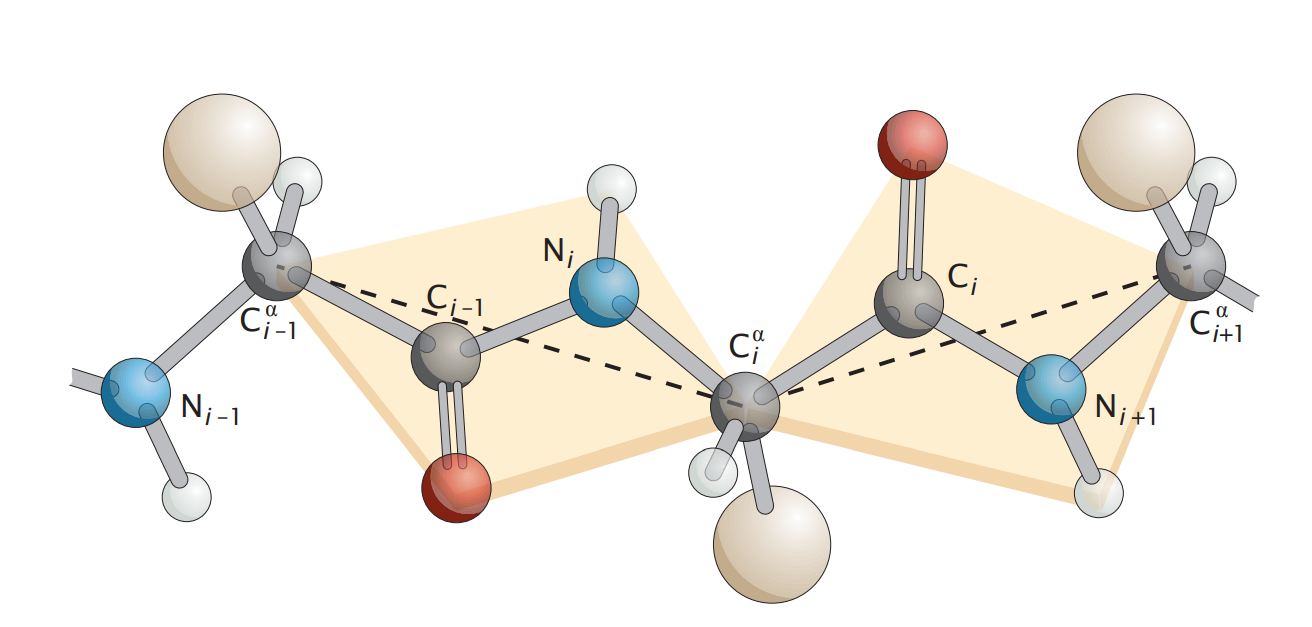
\includegraphics[width=\textwidth]{planar.png}
	\caption{sp2 hybridization of backbone C and N (not $C^{\alpha}$). This is an experimental finding which needs to be incorporated into the system: in this way (and by taking into consideration all the knowledge on proteins), the degree of freedom of the system can be reduced.}
	\label{fig:planar}
\end{figure}

	\subsection{Trans and cis}
	Looking at the peptide bond the carbon atom of the carboxylic group $C'$ and the nitrogen $N$ are each bonded to a different $\alpha$-$C$ and a trans or cis conformation can happen.
	Trying to visualize the atoms that belong to the molecules these repel through the Van der Waals interactions, that can be computed through the Lennard-Jones potential (represented in figure \ref{fig:potential}):

	$$U_{Lj}(r) = E_0\biggl[\biggl(\frac{r_0}{r}\biggr)^{12}-2\biggl(\frac{r_0}{r}\biggr)^6\biggr]$$

	Where:

	\begin{multicols}{2}
		\begin{itemize}
			\item $r_0$ is the distance where the energy is minimum.
			\item $r$ is the distance between two atoms.
			\item $r_{min}$ is the distance at which the energy becomes high.
		\end{itemize}
	\end{multicols}

	\begin{figure}[H]

		\centering
		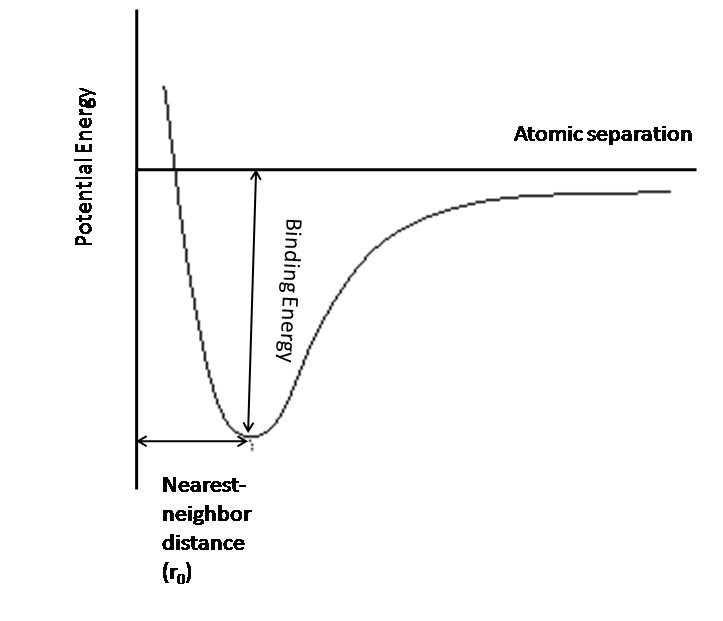
\includegraphics[width=0.5\textwidth]{potential.png}
		\caption{Graphical representation of the energy plotted along the distance between atoms. $r_0$ is the equilibrium distance and it explains the reason why the trans configuration is preferred over the cis configuration}
		\label{fig:potential}
	\end{figure}

	With atoms most of the time the distance between them will be close to $r_0$.
	When decreasing the distance a lot of energy is needed and strain is introduced in the molecule.
	Plotting the values for the energy, $r_0$ and $r_{min}$ the expected distance for each couple of atoms can be seen.
	Focusing on the $C$-$C$ interaction:

	\begin{multicols}{2}
		\begin{itemize}
			\item $r_0 = 3.4\si{\angstrom}$.
			\item $r_{min} = 3.0\si{\angstrom}$.
		\end{itemize}
	\end{multicols}

	When two carbons atoms are below the minimum value the conformation is strained.
	Looking back at the conformation of the peptide bond it can be seen that the cis conformation creates a distance of $2.8\si{\angstrom}$ between the two $\alpha$-$C$, so it is not favourable.
	So the trans conformation is the least energy-hungry and the most present.

	Note that the Lennard-Jones potential is not the only one possible.
	Although it is preferred in most scenarios, other types of potential (e.g., buckingham potential or LJ with different powers) there exist.

\section{The Ramachandran angles}
The planes formed by the peptide bonds can rotate with respect to each other.
So the Ramachandran angles $\phi$ and $\psi$ can be defined between these planes.
For each $\alpha$-$C$:

\begin{multicols}{2}
	\begin{itemize}
		\item $\phi$ describes the rotation around its bond with the nitrogen.
		\item $\psi$ describes the rotation around its bond with the carboxylic group.
	\end{itemize}
\end{multicols}

These are the angles between the subsequent planes.
Some of the angles will require more energy.

	\subsection{Difficulty of rotation}
	It can be seen how a rotation of the $\phi$ angle could cause the two $C'$ to come at a distance of $2.9\si{\angstrom}$ (where $r_{min} = 3.0\si{\angstrom}$.
	On the other hand a rotation of the $\psi$ angle could cause the two $N$ to come at the same distance, but in this case $r_{min}(N-N) = 2.7\si{\angstrom}$.
	In the case of carbon atoms the distance is less than the minimum distance, while in the case of nitrogen it is greater than the minimum allowed value.
	Looking at this it can be seen how the $\psi$ rotation is easier.

	\subsection{Ramachandran plot}
	A Ramachandran plot is a map with the $\phi$ angle on the $x$ axis and the $\psi$ angle on the $y$ axis.
	Because a rotation along the $\phi$ angle is highly disfavoured the angle $0$ is strongly disfavoured and is represented like a black stripe (disallowed region).
	If the amino acids where composed only by carbon and nitrogen atom the Ramachandran map would be the one represented in figure \ref{fig:rama}, where it can be found:

	\begin{multicols}{2}
		\begin{itemize}
			\item A forbidden region in the middle.
			\item Some strained region like for $\psi=0$.
		\end{itemize}
	\end{multicols}

	\begin{figure}[H]
		\centering
		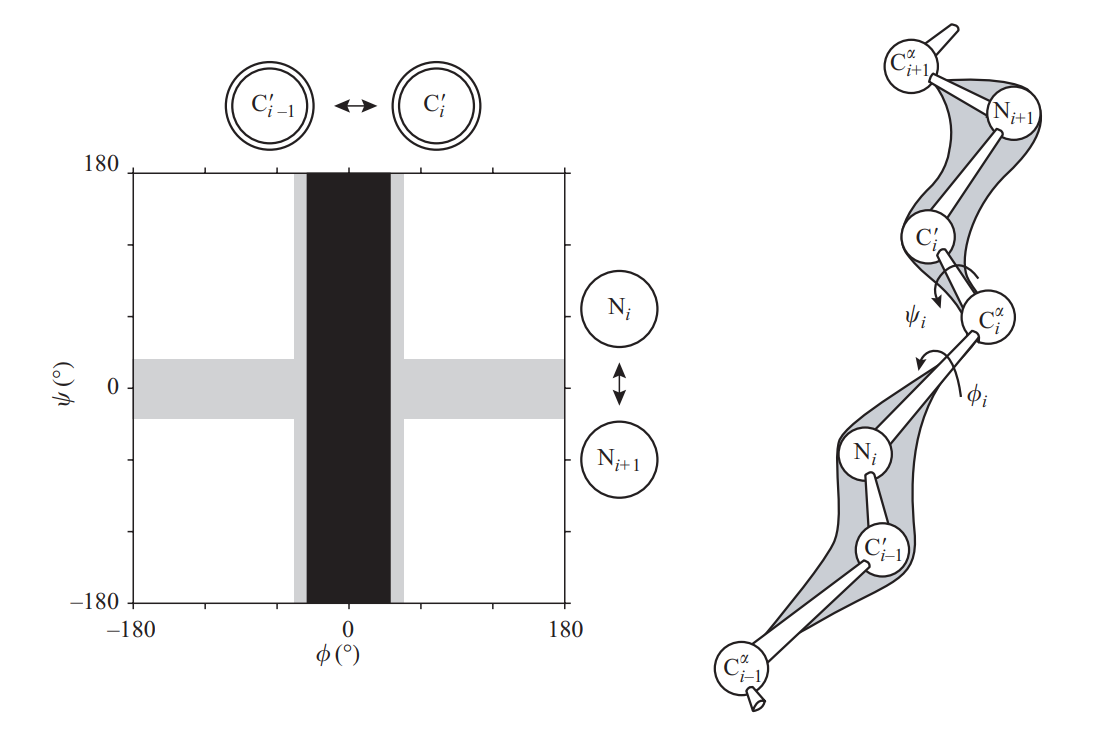
\includegraphics[scale = 0.3]{rama_map.png}
		\caption{This is how Ramachandran plots of the disallowed (black stripe), strained (grey stripe), and fully allowed (white regions) ($\phi$, $\psi$) conformations of the fragment $C^{\alpha}C'N$---$C^{\alpha}$---$C'N-C^{\alpha}$ would look, provided all these atoms had no other atoms attached (right) and atoms of residues $i-1$ and $i+1$ had no interactions.}
		\label{fig:rama}
	\end{figure}

	Looking at a real protein the complexity is increased and the other oxygen and nitrogen atoms are included \ref{fig:ramachandran-complex} and other regions become disallowed due to steady clashes.
	It can be seen how the regions are quite complex.

	\begin{figure}[H]
		\centering
		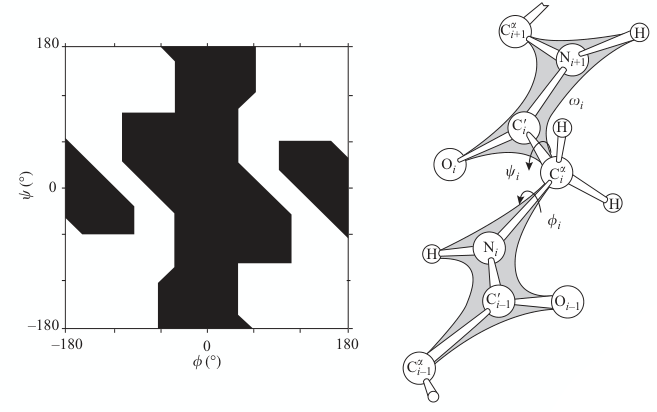
\includegraphics[scale = 0.3]{ramachandran-complex.png}
		\caption{Ramachandran plot of a peptide bond with other atoms.}
		\label{fig:ramachandran-complex}
	\end{figure}

		Looking at a glycine and alanine complex it can be seen in \ref{fig:ala_gly-theo} the space becomes even more complex.

	\begin{figure}[H]
		\centering
		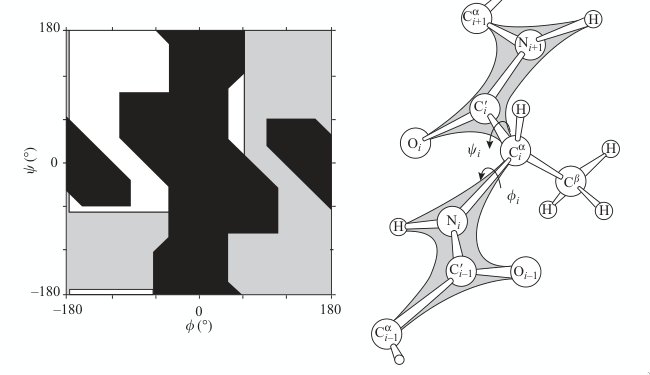
\includegraphics[scale = 0.3]{ala-gly-theo.png}
		\caption{Theoretical representation of a Ramachandran plot of a glycine-alanine complex.}
		\label{fig:ala_gly-theo}
	\end{figure}

	In this case the white regions is very small and a strained region can be seen and the black one.
	Including other residues the allowed region reduces \ref{fig:ramachandran-final}.
	This is due to the presence of larger residues.

	\begin{figure}[H]
		\centering
		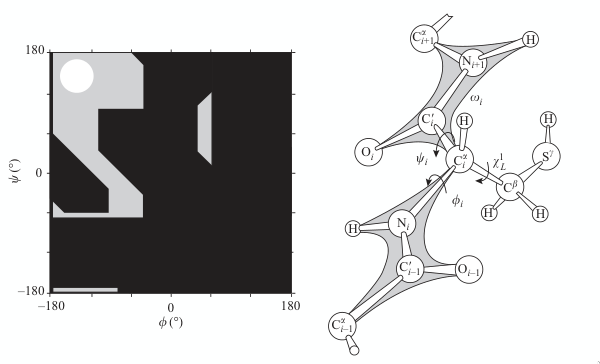
\includegraphics[scale = 0.3]{ramachandran-final.png}
		\caption{Ramachandran plot of a larger residue.}
		\label{fig:ramachandran-final}
	\end{figure}

		\subsubsection{Observed Ramachandran plot}
		Trying to plot for each amino acid its angles an amino acid is represented as a dot.
		Most of the points fall inside of the allowed regions but there are some outliers.
		In some conformation the protein forces the amino acid to assume strange conformations.
		This is done to check if the structure places the amino acids in a proper way.
		A typical observed Ramachandran plot looks like the one in \ref{fig:ala_gly}.

		\begin{figure}[H]
			\centering
			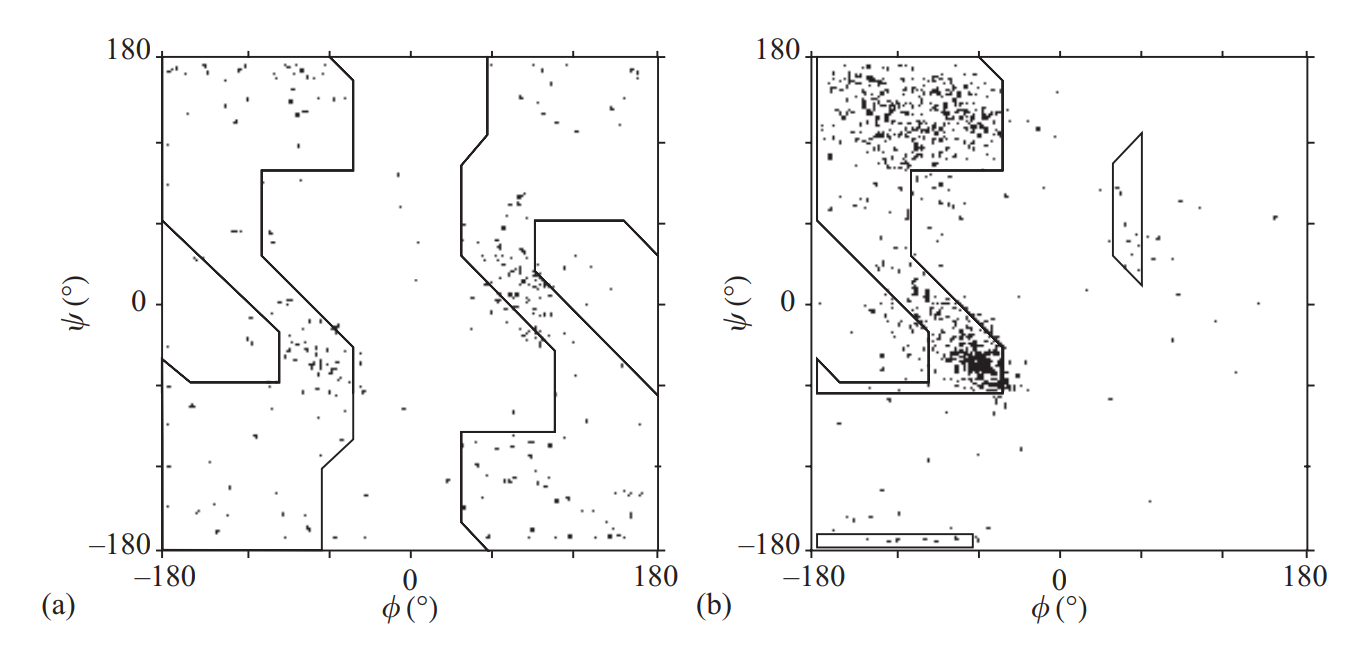
\includegraphics[width=\textwidth]{ala_gly.png}
			\caption{Observed conformations (dots) of glycine (a) and of other amino acid residues (b) in proteins. The sterically allowed regions are contoured.}
			\label{fig:ala_gly}
		\end{figure}


\section{Contact map of proteins}
Starting from the coordinates a contact map can be built.
It is a matrix that map all the contact between the amino acids.
A primary structure can be represented as a collection of beads which will be in contact in the 3D structure.
A square matrix can be built such that each entry in the matrix will determine whether there is a contact or not.
This matrix will be symmetric with diagonal elements with value $1$ and two parallel diagonals for the neighbouring amino acids (figure \ref{fig:contact}).
Secondary structures will have specific signatures:

\begin{multicols}{2}
	\begin{itemize}
		\item $\alpha$-helices: is usually represented by a line parallel to the diagonal.
			This is because the amino acids $i$ is interacting with $i+4$.
		\item $\beta$-strands: the situation is complicated.
			For parallel $\beta$ sheets can be parallel to the diagonal.
			For anti-parallel it can be anti-parallel to the diagonal.
	\end{itemize}
\end{multicols}


\begin{figure}[H]
			\centering
			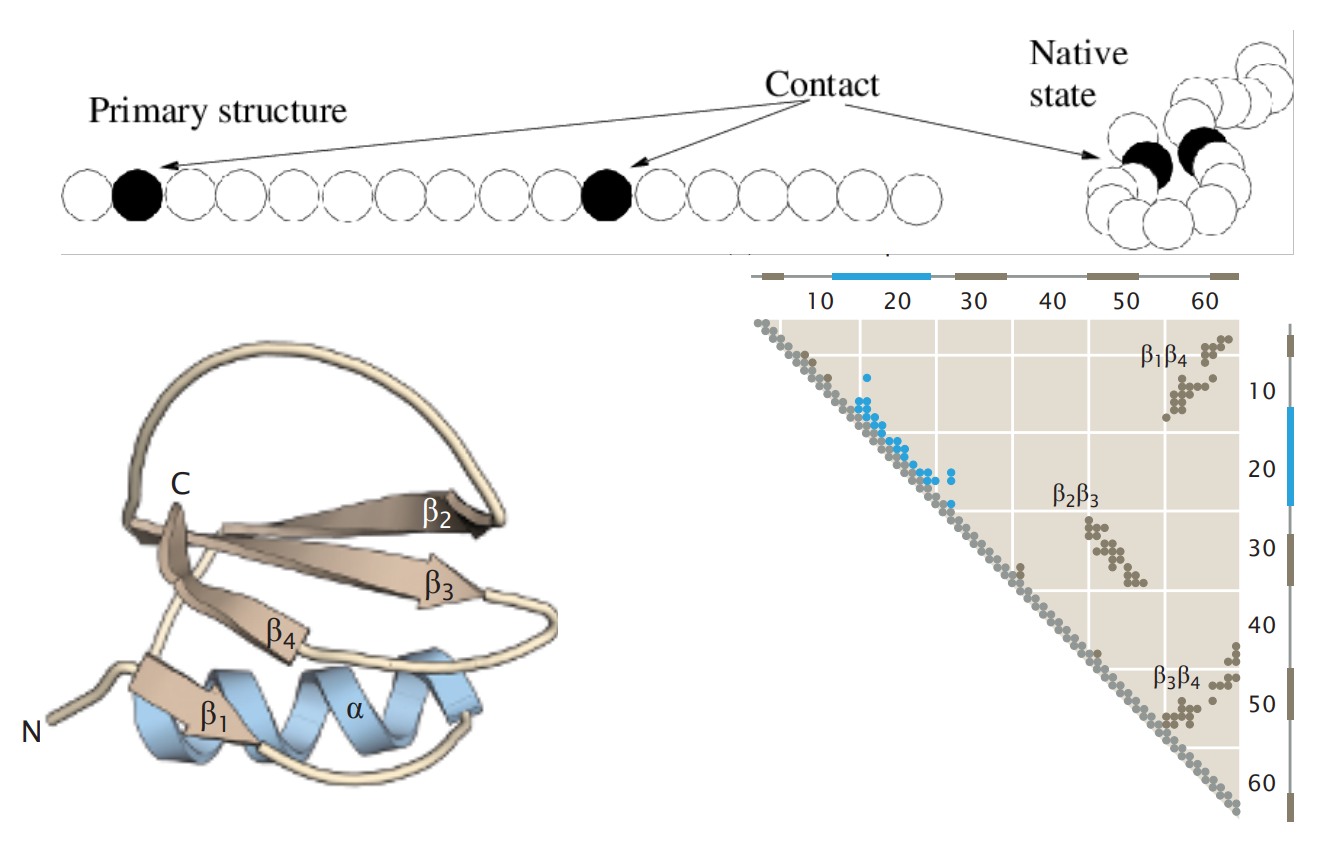
\includegraphics[width=\textwidth]{contact.png}
			\caption{Example of a contact map for a protein.}
			\label{fig:contact}
			\end{figure}


	\subsection{Defining a contact}
	The contact between two amino acids needs to be defined.
	To do so the distance between $\alpha$-$C$ or the distance between the tail of the residue and an $\alpha$-$C$.
	There is also the need to make a trade-off between computational speed and cost.
	Also the dimension of the protein need to be considered when choosing the distance.

\section{Topology diagram}
Having found the secondary structures with a contact map a topology diagram help to understand how those interact with each other (figure \ref{fig:topology}).
In a topology diagram the start is the $N$ terminus and the end the $C$ terminus.
$\beta$-strands are represented as arrows.
If the strands always change direction they will form an anti-parallel $\beta$-sheet.
$\alpha$-helices are represented as small cylinder.
Usually color codes represent the nature of the structure.
This helps with numbering of the secondary structures.

\begin{figure}[H]
			\centering
			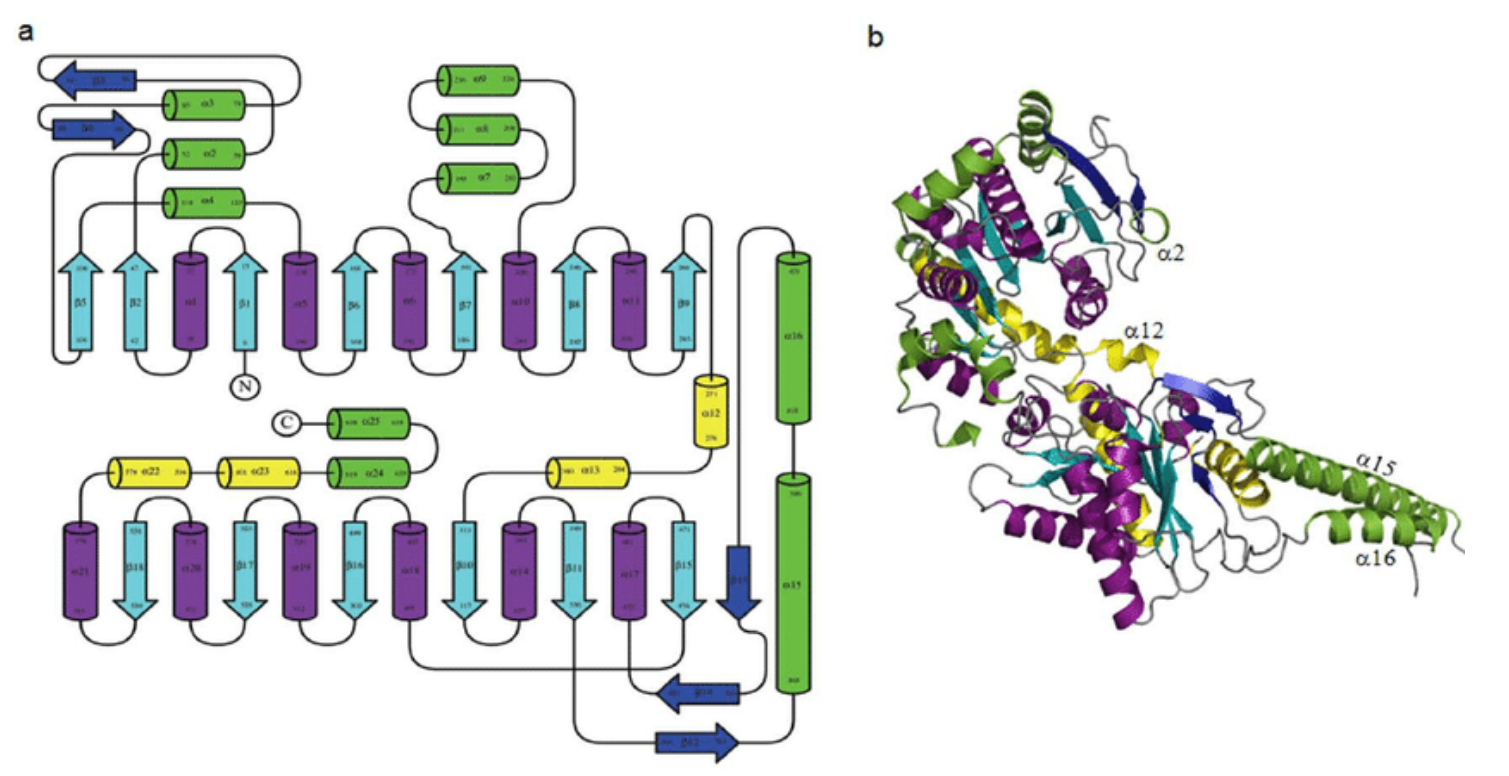
\includegraphics[width=\textwidth]{topology.png}
			\caption{The topology of a protein structure is a highly simplified description of its fold including only the sequence of secondary structure elements, and their relative spatial positions and approximate orientations. This information can be embodied in a two-dimensional diagram of protein topology, called a TOPS cartoon. (from pubmed)}
			\label{fig:topology}
			\end{figure}


\section{Coordinates}
The coordinates of all atoms in a protein are described in a PDB file.
This is a tabulated file containing different columns:

\begin{multicols}{2}
	\begin{itemize}
		\item Atom record: ATOM.
		\item Atom number: a unique identifier for the atom.
		\item Atom identifier: an identifier for the type of atom.
		\item Amino type: the amino acid from which the atom is from.
		\item Chain identifier: identifier for the chain.
		\item Residue sequence number: the number of the residue in the chain.
		\item $x$, $y$, $z$: the coordinates in angstrom.
		\item Occupancy: the probability of an atom to be in that space (confidence space).
		\item B-factor: how mobile that atom is in the crystal, it represent the noise in the x-ray diffraction map (it represents the fluctuations for the coordinate of the atoms. For example, loops in trans-membrane proteins are very mobile and a high B-factor is to be expected).
		\item Element symbol: the symbol of the element of the atom.
	\end{itemize}
\end{multicols}

Once the coordinates of a protein is obtained, some geometrical properties can be directly computed.

	\subsection{Protein centre of mass}
	The protein centre of mass is the average position for the protein centre.
	It is an average weighted by the mass of the atom.

	$$\vec{R}_{cm} = \frac{\sum\limits_{i=1}^Nm_i\vec{r}_i}{\sum\limits_{i=1}^Nm_i}$$

	\subsection{Radius of gyration}
	Once the centre of mass is known the radius of gyration can be computed.
	This measures the size of the protein as if it was a sphere.
	It is a good indication of the globular size of a protein.
	It also indicates an elongating/shrinking behaviour, and useful to check whether a protein is going toward equilibrium in the simulation.
	The distance of each atom and the centre of mass is computed and the square is taken, weighted with the mass of the atom.

	$$R_g = \sqrt{\frac{\sum\limits_{i=1}^Nm_i(\vec{r}_i-\vec{R}_{cm})^2}{\sum\limits_{i=1}^Nm_i}}$$

	\subsection{Comparing protein structures}
	Proteins have structures that loop in a similar way, with similar regions within each other.
	To quantify the similarity between the protein structure a procedure needs to be followed:

		\begin{itemize}
			\item Select common regions: a $1$-$1$ correspondence between amino acid need to be found: the parts present only in one protein are not considered.
				A correspondence is built between the common regions on the single amino-acids.
				These can be different, usually the coordinates are confronted between the $\alpha$-$C$ atom and the residue is not considered.
				One of the things that can be done is to look at the secondary structures and add loops only when they look similar.
			\item Align the two structures: compute the centre of mass of the two proteins and translate the proteins so the centre of masses coincide.
			\item Finding the optimal rotation: the principal axes are computed and the proteins are rotated so that they superimpose.
				Once the optimal rotation is obtained the difference can be quantified.
			\item Compute RMSD (root mean square deviation): take the coordinates of the amino-acid $i$ in protein $A$ and $B$, their squared difference is computed and an average over all amino acid is computed and squared:

				$$RMSD = \sqrt{\frac{1}{N}\sum\limits_{i=1}^N(\vec{r}_{Ai}-\vec{r}_{Bi})^2}$$
				the RMSD is a length, usually in angstrom scale.
				This can be done for two proteins or for the protein taken at two different time step in a molecular dynamics simulation:

				$$RMSD(t) = \sqrt{\frac{1}{N}\sum\limits_{i=1}^N(\vec{r}_{i}(t)-\vec{r}_{i}(0))^2}$$

				Now the $RMSD$ can be plotted with respect to time.
				It can be seen how at $t=0$ $RMSD=0$ and after the value will increase.
				When the number reaches a plateau the protein should be in equilibrium.
				The plateau can jump to another value, meaning that the state is a meta-stable state of the protein, or the protein has more stable states or a loop is making something.
				This value is assigned to very complicated structures and different structures can have the same $RMSD$.
				Clearly, a reference structure needs to be picked.
				In MD of a protein evolving in time, the reference structure is the initial configuration of the protein.
				One can also decide to focus on a specific region.
				The $RMSD$ is an indicator of equilibrium: it is a necessary but not sufficient condition.
		\end{itemize}

		\begin{figure}[H]
			\centering
			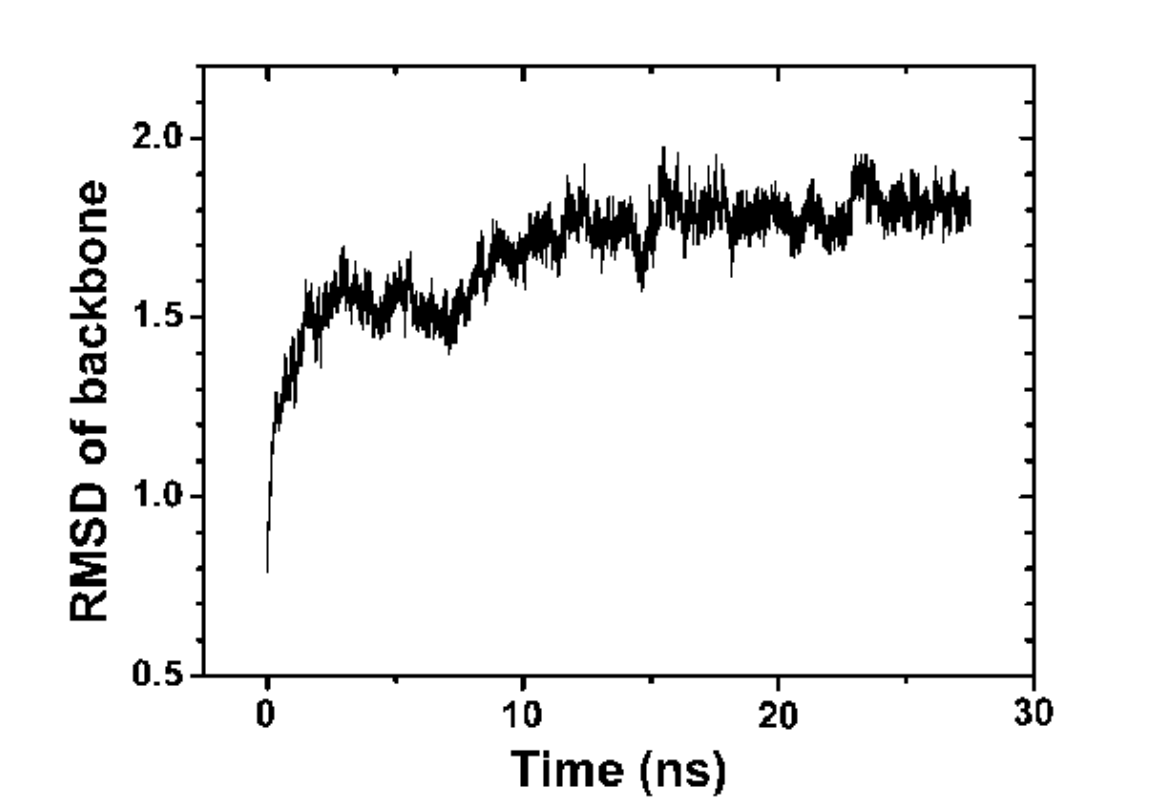
\includegraphics[scale = 0.3]{rmsd.png}
			\caption{RMSD of the backbone ($C^{\alpha}$, $N$, ...). We can see the typical steep jump a fluctuations towards the end of the plot. However, this is not enough to state that the protein reached equilibrium.}
			\label{fig:rmsd}
			\end{figure}


	\subsection{Native state}
	The native state is the functional state of a protein.
	It is not the state found for a crystallized protein, but only closely related to it, it is rather an ensemble in space and time of structures.
	This is due to proximity effect and the fact that the protein is not a static system.
	Proteins are extremely flexible and are moving a lot because the temperature corresponds to a constant movement of water molecule around causes movement in the protein.
	The native state is an ensemble of closely related states, all compatible with the conditions of the situation studied.
	Proteins need to be studied in the isothermal-isobaric ensemble.
	All the calculation need to be done at constant temperature and pressure.
	The native state is so a collection of functional state.

	In the case of the unfolded state the possibilities are too many to sample all of them.

	\subsection{RMSF}
	The flexibility of each amino acid can be computed.
	With flexibility is intended the movement of amino acid with respect to one another.
	In the $\alpha$-helix, for example, less fluctuation is expected, while in loops more fluctuation is expected.
	This quantity is computed in the root mean squared fluctuation, which will be computed for each amino acid in the protein.
	With $f$ referring to the frame, let:

	\begin{itemize}
		\item $\langle \vec{r}_i\rangle = \frac{1}{M}\sum\limits_{f=1}^M\vec{r}_{i,f}$, the average position of atom $i$.
		\item $\Delta\vec{r}_{i,f} = \vec{r}_{i,f}-\langle\vec{r}_i\rangle$, the displacement of each atom in each frame with respect to its average.
		\item $\langle \Delta\vec{r}_o^w\rangle = \frac{1}{M}\sum\limits_{f=1}^M(\vec{r}_{i,f}-\langle\vec{r}_i\rangle)^2$, the average squared distance over the frames.
	\end{itemize}

	So, the root mean squared fluctuation is:

	$$RMSF_i = \sqrt{\langle\Delta\vec{r}_i\rangle^2}$$

	Plotting the $RMSF$ with respect to residue number and the more mobile residue can be identified.
	This can be mapped onto the sequence so loops, helices and strands can be recognized.
	Usually the fluctuating part correspond to loops.
	The terminus have the highest $RMSF$.

		\subsubsection{B-factors}
		$RMSF$ can be translated into B-factors.
		They are the Debye-Waller factors and are a scaled version of the $RMSF$ squared.
		So the result of a simulation can be compared with the B-factor and a strong correspondence can be seen.
		The differences are due to the fact that the crystal is a different environment with respect to the normal one and packing effect can happen (some regions of the protein can interact with the image of the protein in the crystal).

		$$B_i = \frac{8\pi^2}{3}\langle\Delta\vec{r}_i^2\rangle = \frac{8\pi^2}{3}RMSF^2_i$$

  % \graphicspath{{chapters/03/images/}}
\chapter{Semi-empirical force fields}

\section{Introduction}
A protein system can be modelled using a force field, a description of the interactions between elements in the system.
A simulation needs a topology file which describes all of the interactions, the connecting information between atoms and the kind of force field that will be used.
To model protein systems semi-empirical force field are used.
The formula used in these kind of force fields are not rigorous: all the results from a simulation need to be validated through an experiment.

	\subsection{Potential energy surface}
	The state of any system can be described through a potential energy surface.
	The minima of the potential energy surface represents states in which the system will spend most of its time.
	The equilibrium state is found in the global minima of the surface.
	Lots of local minima are usually found on the surface and the system will jump between them during a simulation, with a frequency that depends on the deepness of the minima and the temperature of the environment.
	Statistical mechanics is necessary to compute the potential energy and the free energy surfaces at finite temperature, or when the jumping frequency is not zero.

		\subsubsection{Entropy}
		When dealing with these kind of computations entropy needs to be taken into account.
		To do so the conformational space, or the phase space, of the system needs to be explored so that compatible conformations for a certain condition can be found.

	\subsection{Types of force fields}
	Force fields can be categorized as:

	\begin{multicols}{2}
		\begin{itemize}
			\item All atoms: one atom corresponds to one bead.
			\item More atoms: more atoms correspond to one bead.
			\item Corse grained: groups of atoms correspond to one bead.
			\item Polarizzarle force fields: point charges are variables.
		\end{itemize}
	\end{multicols}

	As a golden rule parameters from different force fields should never be mixed.


\section{Computing the potential energy between bonded atoms}
When computing the potential energy of an atom its interactions with the other with which it forms a chemical bond needs to be considered.
The chemical bond can assume different conformations, each with a different value of potential energy.
Because the objective is to consider conformational transitions, the system will be completely modelled using classical mechanics, so bonds are unbreakable.
The potential energy surface used to describe an unbreakable bond can be seen in figure \ref{fig:chem-bond}.

\begin{figure}[H]
	\centering
	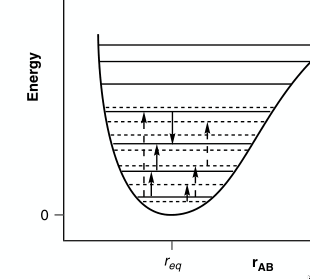
\includegraphics[width=0.5\textwidth]{chem-bond}
	\caption{Typical potential energy of a chemical bond}
	\label{fig:chem-bond}
\end{figure}

	\subsection{Bond stretching}
	During bond stretching the distance of two bonded atoms changes.
	To model this process consider the typical potential energy for a chemical bond in figure \ref{fig:chem-bond}.
	Let $r_{eq}$ the distance for which the energy is minimal, or where the equilibrium is.
	Moving from it the energy increases.
	When close to the minimum the well can be assumed symmetric.
	Asymmetry arises far from the minimum: it can be seen how the left part is steeper.
	Using a Taylor expansion the potential energy is approximated at point $r$ by taking the value at the equilibrium and then constructing all the corrections:

	$$U(r)=U(r_{eq}) + \frac{dU}{dr}\biggr\vert_{r=r_{eq}}(r-r_{eq})+\frac{1}{2!}\frac{d^2U}{dr^2}\biggr\vert_{r=r_{eq}}(r-r_{eq})^2+\frac{1}{3!}\frac{d^3U}{dr^3}\biggr\vert_{r=r_{eq}}(r-r_{eq})^3+\cdots$$

	Considering this expansion:

	\begin{multicols}{2}
	  \begin{itemize}
	    \item The first term is the value at equilibrium multiplied by the distance.
			\item The second term is the correction for the second derivative and so on.
	  \end{itemize}
	\end{multicols}

	Now a number of assumptions can be made:

	\begin{multicols}{2}
	  \begin{itemize}
	    \item If the potential is symmetric the first term is $0$ as it happens near the equilibrium.
				This makes the first term negligible.
			\item If the minimum is shallow the third term is $0$ and happens near the equilibrium.
				This makes the third term negligible.
	  \end{itemize}
	\end{multicols}

	\begin{align*}
		U(r)&=U(r_{eq}) + \xcancel{\frac{dU}{dr}\biggr\vert_{r=r_{eq}}(r-r_{eq}})+\frac{1}{2!}\frac{d^2U}{dr^2}\biggr\vert_{r=r_{eq}}(r-r_{eq})^2+\xcancel{\frac{1}{3!}\frac{d^3U}{dr^3}\biggr\vert_{r=r_{eq}}(r-r_{eq})^3}+\cdots\\
	\end{align*}

	So that in the end the typical harmonic potential is obtained:

	$$U(r_{AB}) = \frac{1}{2}k_{AB}(r_{AB}-r_{AB,eq})^2$$

	Considering that:

	\begin{multicols}{2}
	  \begin{itemize}
			\item $k$ is related to $\frac{d^2 U}{dr^2}$.
			\item The distances and $k$ are unique for each couple of atoms.
				An important issue for these parameters is transferability: these type of parameters need to be computed for each type of force field.
	  \end{itemize}
	\end{multicols}

		\subsubsection{Anharmonic force constant}
		Considering that the shape is not completely symmetric the third order term can be re-inserted in the formula when necessary.
		This introduces an asymmetry in the system, or an anharmonic force constant:

		$$U(r_{AB}) = \frac{1}{2}[k_{AB}+k^{(3)}_{AB}(r_{AB}-r_{AB, eq})](r_{AB}-r_{AB, eq})^2$$

		\subsubsection{Quartic correction}
		Also the fourth order term can be inserted for better accuracy:

		$$U(r_{AB}) = \frac{1}{2}[k_{AB}+k^{(3)}_{AB}(r_{AB}-r_{AB, eq}) + k^{(4)}_{AB}(r_{AB}-r_{AB,eq})^2](r_{AB}-r_{AB, eq})^2$$

		\subsubsection{Morse potential}
		The Morse potential is used in implicit solvent simulation.
		The exponential allows to describe screen interactions that happen with the implicit solvent.
		This is more difficult to compute, but it is also useful for soft or coarse-grained systems.

		$$U(r_{AB}) = D_{AB}\left[1-e^{-\alpha_{AB}(r_{AB}-r_{AB,eq})^2}\right]$$

	\subsection{Valence angle bending}
	When an atom makes multiple bonds with different atom the angle between the bonds can fluctuate around an equilibrium value.
	These events are described as valence angle bending.
	A valence angle is represented in \ref{fig:valence-angle-bending}.

	\begin{figure}[H]
		\centering
		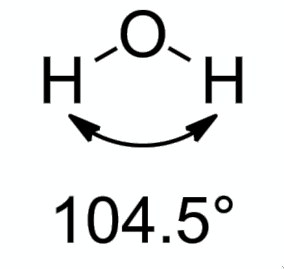
\includegraphics[width=0.3\textwidth]{valence-angle-bending}
		\caption{A valence angle}
		\label{fig:valence-angle-bending}
	\end{figure}

	In order to describe valence angle bending a Taylor expansion introducing an equilibrium angle is built.
	The first order term is not considered as it will be equal to $0$.
	Then the second introduces the harmonic potenital and the third for the anharmonic one, in principle also the quartic correction could be added.
	This formula is similar to the previous one but all the constant have to be described between each triplet of atoms:

	$$U(\theta_{ABC}) = \frac{1}{2}[k_{ABC}+k^{(3)}_{ABC}(\theta_{ABC}-\theta_{ABC,eq})+k^{(4)}_{ABC}(\theta_{ABC}-\theta_{ABC,eq})^2+\cdots](\theta_{ABC}-\theta_{ABC, eq})^2$$

		\subsubsection{Multiple minima}
		Another thing to consider when studying valence angle bending is that angles do not vary continuously: they wrap around at $\pi$ and $0$.
		This introduces a problem as the Taylor expansion cannot account for this event.

			\paragraph{Fourier expansion}
			To solve this problem the potential energy can be modelled thought a Fourier expansion.
			This operation introduces a periodic function that contains oscillations around a period, allowing to model any possible periodic potential, as the one for angles.

			\paragraph{Valence angle bending with a Fourier expansion}
			To parametrize the valence angle bending interaction a Fourier term is introduced, such that the terms are labelled with $j$.
			The amplitude, which multiplies each Fourier component decreases with $j$ and a cut-off on it is given, so to consider only low-frequency components.
			Now the potential energy for a valence angle bending interaction can be described by:

			$$U(\theta_{ABC}) = \sum\limits_{\{j\}_{ABC}}k^{fourier}_{j,ABC}[1+\cos(j\theta_{ABC}+\psi_j)]$$

			Where:

			\begin{multicols}{2}
			  \begin{itemize}
			    \item $\psi_j$ is the phase angle.
					\item The amplitude is computed as:

						$$k_{j, ABC}^{fourier} = \frac{2k^{harmonic}_{ABC}}{j^2}$$

			  \end{itemize}
			\end{multicols}

	\subsection{Torsions}
	Let $A, B, C$ and $D$ be $4$ atoms, bound according to $A->B->C->D$, like in figure \ref{fig:torsions}.
	Torsions describe the relative rotations of atoms $A$ and $D$ around the bond between $C$ and $D$.

	\begin{figure}[H]
		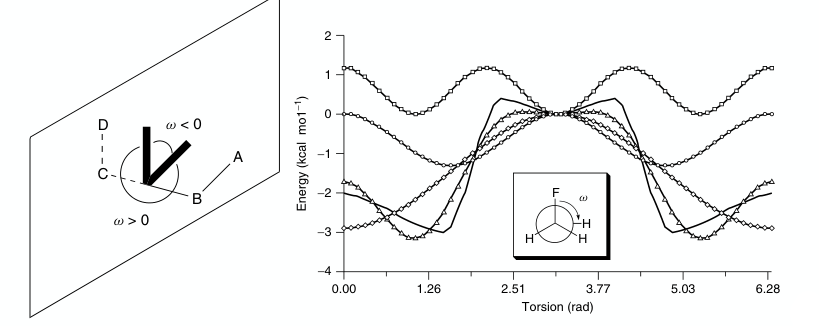
\includegraphics[width=\textwidth]{torsions}
		\caption{An example of torsion}
		\label{fig:torsions}
	\end{figure}

	To model this movement the planes $ABC$ and $BCD$ are built and the angle $\omega$ between them is considered.
	$\omega$ will describe the torsion around the bond.
	The angle is computed as the angle between the vectors perpendicular to the planes.
	The potential is computed through a Fourier expansion because it is periodic:

	$$U(\omega_{ABCD}) = \frac{1}{2}\sum\limits_{\{j\}_{ABCD}}V_{j,ABCD}\left[1+(-1)^{j+1}\cos(j\omega_{ABCD}+\psi_{j,ABCD})\right]$$

	All the possible groups of $4$ atoms, considering permutations and repetitions need to be parametrized to describe this potential.

		\subsubsection{Improper torsions}
		Improper torsions are a particular type of torsion that happens when the four atoms $A, B, C$ and $D$ are bound according to $A->B->C$ and $B->D$, like in figure \ref{fig:improper-torsions}.

		\begin{figure}[H]
			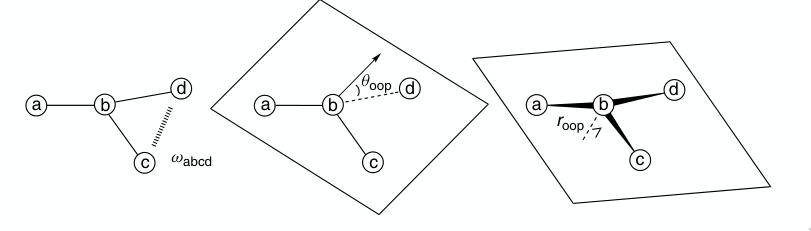
\includegraphics[width=\textwidth]{improper-torsions}
			\caption{An example of improper torsion}
			\label{fig:improper-torsions}
		\end{figure}

		$B$ can be in the same plane of $A, C, D$ or it can pop out.
		In this case two planes are built, usually $ABC$ and $BCD$ and the angle $\omega$ between them is considered.
		The potential will describe the energy of the angle.
		The angle can be computed as the out of plane angle $OOP$, obtaining the equation for the plane $ACD$ and computing how much $B$ is out of that plane.
		The potential is again described through a Fourier expansion:

		$$U(\omega_{ABCD}) = \frac{1}{2}\sum\limits_{\{j\}_{ABCD}}V_{j,ABCD}[1+(-1)^{j+1}\cos(j\omega_{ABCD}+\psi_{j,ABCD})]$$

		To parameterize this potential all possible groups of an atom connected with $3$ others need to be considered.
		The $sp^2$ hybridization constraints all the atoms in a plane.

\section{Non bonded interactions}

	\subsection{Van der Waals interactions}
	Van der Waals interactions happen whenever two atoms come close to one another without any chemical bond connecting them.
	It is a dispersion interaction and depends on the correlation of the electron clouds.
	This happens even if the electrons are not shared between atoms and depend only on the distance between them.
	The potential energy of a Van der Waals interaction is visualized in figure \ref{fig:van-der-waals}.
	Van der Waals interactions are a type of attractive forces that decrease with the $6$th power of the distance and it is closely related to a repulsion.
	The repulsion is due to Pauli's exclusion principle: whenever two atoms come close an energy level becomes occupied and it stops them to become closer.
	This is difficult to compute, so it is modelled through an hard limit, modelled by the $12$th power of the distance, making the energy become very high whenever the distance becomes less than the equilibrium.

	\begin{figure}[H]
		\centering
		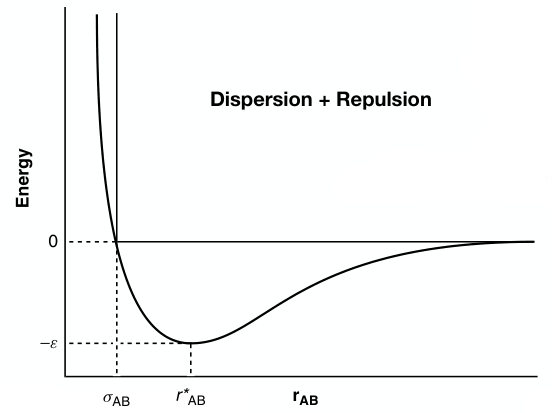
\includegraphics[width=0.5\textwidth]{van-der-waals}
		\caption{Energy of a Van der Waals interaction}
		\label{fig:van-der-waals}
	\end{figure}

		\subsubsection{Lennard-Jones potential}
		The Lennard-Jones potential models both the attraction due to the Van der Waals interaction and the repulsion due to Pauli's exclusion principle.
		The corresponding formula is cheap to compute but has no physical basis:

		\begin{align*}
			U_(r_{AB}) &= \frac{a_{AB}}{r^{12}_{AB}}-\frac{b_{AB}}{r^6_{AB}}=\\
								 &= 4\epsilon_{AB}\biggl[\biggl(\frac{\sigma_{AB}}{r_{AB}}\biggr)^{12}-\biggl(\frac{\sigma_{AB}}{r_{AB}}\biggr)^6\biggr]
		\end{align*}

		And the distance with minimum energy or equilibrium is:

		$$r^*_{AB} = 2^{\frac{1}{6}}\sigma_{AB}$$

		Where $\sigma_{AB}$ is the Van der Waals radius, where the energy is $-\epsilon$.
		A value of $\sigma_{AB}$ have to be introduced for any couple of types of atoms.

		\subsubsection{Morse potential}
		The Morse potential is usually used with coarse grained systems or with soft-matter simulations.
		This potential has the same features of the Lennard-Jones potential:

		$$U(r_{AB}) = D_{AB}[1-e^{-a_{AB}(r_{AB}-r_{AB,eq})^2}]$$

		\subsubsection{Hill potential}
		The Hill potential is usually used with coarse grained systems or with soft-matter simulations.
		This potential has the same features of the Lennard-Jones potential:

		$$U(r_{AB}) = \epsilon_{AB}\biggl[\frac{6}{\beta_{AB}-6}e^{\beta_{AB}\frac{1-r_{AB}}{r^*_{AB}}}-\frac{\beta_{AB}}{\beta_{AB}-6}\biggl(\frac{r^*_{AB}}{r_{AB}}\biggr)^6\biggr]$$

		\subsubsection{Scaling for already accounted interactions}
		In some force fields $1$-$4$ interactions are reduced by a scaled factor, while in other are completely removed.
		This is because in these force fields the torsions are modelled such that they already take into account these proximity effects.

	\subsection{Electrostatic interactions}
	Electrostatic interactions happen between charged or polar molecules.
	To model these kind of interactions the distribution of charges needs to be described.
	In principle a multiple expansion should be performed.
	The shape of the clouds of charges should be given for each molecules and each interaction should be described by the matrix multiplication of all the matrices:

	$$U_{AB} = \vec{M}^{(A)}V^{(B)}$$

	Now, summing over all molecules:

	$$U_{AB} = \sum\limits_{A}\sum\limits_{B>A}\vec{M}^{(A)}\vec{V}^{(B)}$$

	This is a very costly procedure but provides accurate results.

		\subsubsection{Point like charges}
		To make the computation easier molecules are represented as point-like partial charges.
		Each atom in a molecule is assumed to be point like and to have a partial charge.
		The electron cloud is displaced toward the negative cloud and away from the positive one.
		In this way the distribution of charges can be represented by numbers placed on each atom.
		Once this is done an electric charge is associated with each bead and the Coulomb interaction is used to compute the energy:

		$$U_{AB} = \frac{q_Aq_B}{\epsilon_{AB}r_{AB}}$$

		Where $\epsilon_{AB}$ is the dielectric constant and depends on the type of solvent ($1$ for explicit ones).

		\subsubsection{Dipolar interactions}
		Dipolar interaction can be included when considering electrostatic forces.
		These formulae are mostly used in corse grained models: approximation of single charges one a bead cannot be made.
		The interaction takes a functional form with a number of parameters:

		Because in that case the approximation of single charges on a bead cannot be made and dipoles are considered.
		In this case a functional form and the parameters need to be included.
		The energy is computed as:

		$$U_{AB/CD} = \frac{\mu_{AB}\mu_{CD}}{\epsilon_{AB/CD}r^3_{AB/CD}}(\cos\chi_{AB/CD}-3\cos\alpha_{AB}\cos\alpha_{CD})$$

		Where:

		\begin{multicols}{2}
		  \begin{itemize}
		    \item $\mu$ is the dipole of two molecules.
				\item $\epsilon_{AB/CD}$ is the dielectric constant.
				\item The cosine term represents the orientation of the two dipoles.
		  \end{itemize}
		\end{multicols}

		\begin{figure}[H]
			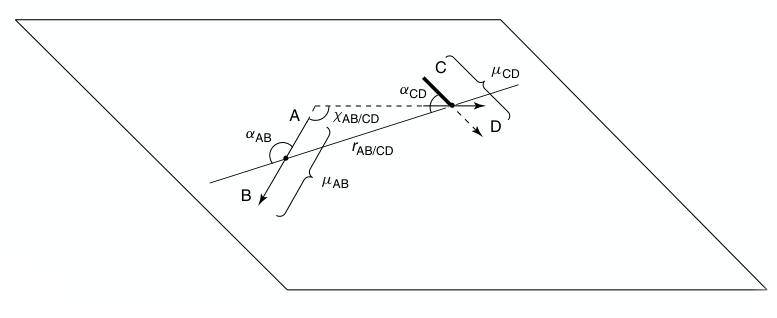
\includegraphics[width=\textwidth]{dipolar-interactions}
			\caption{An example of a dipolar interaction}
			\label{fig:dipolar-interactions}
		\end{figure}

		\subsubsection{Dielectric constants}
		The dielectric constant changes depending on the type of interaction the atom.
		For example:

		$$\epsilon_{AB} = \begin{cases}\infty&\text{ if }A\land B\text{ are 1,2- or 1,3-related}\\3.0&\text{ if }A\land B\text{ are 1,4-related}\\1.5&\text{otherwise}\end{cases}$$

		These scaling factors depend on the force field chosen.

\section{Cross terms}
Different type of interactions depend between each other, so all the possible degree of freedom should be considered together:

\begin{align*}
	U(\vec{q}) = &U(\vec{q}_{eq}) + \sum\limits_{i=1}^{3N-6}(q_i-q_{i,eq})\frac{\partial U}{\partial q_i}\biggr\vert_{\vec{q}=\vec{q}_{eq}} + \\
							 &+\frac{1}{2!}\sum\limits_{i=1}^{3N-6}\sum\limits_{j=1}^{3N-6}(q_i-q_{i,eq})(q_j-q_{j,eq})\frac{\partial^2 U}{\partial q_i\partial q_j}\biggr\vert_{\vec{q}=\vec{q}_{eq}} +\\
							 &=\frac{1}{3!}\sum\limits_{i=1}^{3N-6}\sum\limits_{j=1}^{3N-6}\sum\limits_{k=1}^{3N-6}(q_i-q_{i,eq})(q_j-q_{j.eq})(q_k-q_{k,eq})\frac{\partial^3 U}{\partial q_i\partial q_j\partial q_k}\biggr\vert_{\vec{q}=\vec{q}_{eq}} + \cdots
\end{align*}

This is done by starting from a Lagrangian describing all the interaction and compute all the terms.
In practice, besides some force fields, everything is done without considering them:

$$U(r_{AB}, \theta_{ABC}) = \frac{1}{2}k_{AB,ACB}(r_{AB}-r_{AB, eq})(\theta_{ABC}-\theta_{ABC, eq})$$

\section{Parametrization}
All the interactions need a large set of parameters to be computed, which grows with the number of atoms $N$ as:

$$p = N + (N-1)+(N-2)+\cdots = N\frac{N+1}{2}$$


	\subsection{Obtaining the parameters}
	The parameters are obtained comparing experimental data (from which the term semi-empirical) with the results of a simulation.
	Then the penalty function is introduced:

	$$Z = \biggl[\sum\limits_{i}^{observables}\sum\limits_{j}^{occurrences}\frac{(calc_{i,j}-expt_{i,j})^2}{w_i^2}\biggr]^{\frac{1}{2}}$$

	This is summed over all the data from all the observables.
	Then it is minimized by changing the simulation's parameters until a reasonable compromise is reached.
	This is the reason for the constant update of the force fields.

	\subsection{Reducing the number of parameters}
	To reduce the number of parameters, they are factorized so that they need to be defined only for each atom:

	\begin{align*}
		\sigma_{AB} &= \sigma_A+\sigma_B\\
		\epsilon_{AB} &= (\epsilon_A\epsilon_B)^{\frac{1}{2}}
	\end{align*}

	\subsection{Geometry optimization}
	It may happen that two atoms are too close to each other at the start of a simulation, leading to high forces, kicking out the atom and causing the simulation to explode.
	Geometry optimization is done to obtain the parameters or to minimize them so to avoid high forces values at the start of a simulation.
	To do so the gradient of the energy is computed and the system is moved toward the minimum energy.
	The derivative need to be computed of $U$ with respect to each component in the system.

	$$\vec{g}(\vec{q}) = \begin{bmatrix} \frac{\partial U}{\partial q_1} \\ \frac{\partial U}{\partial q_2} \\ \vdots \\ \frac{\partial U}{\partial q_n}\end{bmatrix}$$

	Such that the cost reaches the global minimum $J_{min}(\vec{w})$.

		\subsubsection{Derivative of the potential function}
		First the derivatives need to be computed.
		All the potentials are given in term of the mutual distance of two atoms.
		So, considering $x$ the coordinates of a point:

		$$\frac{\partial U}{\partial x_A} = \sum\limits_{i\in A}\frac{\partial U}{\partial r_{Ai}}\frac{\partial r_{Ai}}{\partial x_A}$$

		Taking the derivative of this:

		$$U(r_{AB}) = \frac{1}{2}[k_{AB}+k_{AB}^{(3)}(r_{AB}-r_{AB, eq}) + k_{AB}^{(4)}(r_{AB}-r_{AB, eq})^2](r_{AB}-r_{AB,eq})^2$$

		With respect to the distance:

		$$\frac{\partial U}{\partial r_{Ai}} = \frac{1}{2}[2k_{Ai}+3k_{Ai}^{(3)}(r_{Ai}-r_{Ai, eq}) + 4k^{(4)}_{Ai}(r_{Ai}-r_{Ai, eq})^2](r_{Ai}-r_{Ai, eq})$$

		In order to take the derivative with respect to $r$ the derivative with to $x$ needs to be known:

		$$\frac{\partial r_{Ai}}{\partial x_A} = \frac{x_A-x_i}{\sqrt{(x_A-x_i)^2+(y_A-y_i)^2+(z_A-z_i)^2}}$$

		Then this formula can plugged in according to the chain rule.

		\subsubsection{Newton-Raphson}
		The minimization for geometry optimization is performed as an iterative procedure: the Newton-Raphson.
		Consider $(n)$ as the identifier for the $n$th iteration.
		This allow to obtain iteration $k+1$ via a Taylor expansion of coordinates at iteration $k$:

		$$U(\vec{q}^{(k+1)}) = U(\vec{q}^{(k)}) + (\vec{q}^{(k+1)} -\vec{q}^{(k)})\vec{g}^{(k)} + \frac{1}{2}(\vec{q}^{(k+1)}-\vec{q}^{(k)})H^{(k)}(\vec{q}^{(k+1)}-\vec{q}^{(k)})$$

		Where $H$ is the Hessian matrix:

		$$H_{ij}^{(k)} = \frac{\partial^2 U}{\partial q_i\partial q_j}\biggr\vert_{\vec{q}=\vec{q}^{(k)}}$$

		And:

		$$\frac{\partial U(\vec{q}^{(k+1)})}{\partial q_i^{(k+1)}} = \frac{\partial \vec{q}^{(k+1)}}{\partial q_i^{(k+1)}}\vec{g}^{(k)}+ \frac{1}{2}\frac{\partial \vec{q}^{(k+1)}}{\partial q_i^{(k+1)}}H^{(k)}(\vec{q}^{(k+1)}-\vec{q}^{(k)})+\frac{1}{2}(\vec{q}^{(k+1)}-\vec{q}^{(k)})H^{(k)}\frac{\partial \vec{q}^{(k+1)}}{\partial q_i^{(k+1)}}$$

		So that:

		$$\vec{g}_i^{(k+1)} = \vec{g}_i^{(k)} + [H^{(k)}(\vec{q}^{(k+1)}-\vec{q}^{(k)})]_i$$

		After enough iterations the system reaches a stationary conditions, where the system won't change in successive iterations:

		$$\vec{0} = \vec{g}^{(k)} + H^{(k)}(\vec{q}^{(k+1)}-\vec{q}^{(k)})\Rightarrow \vec{q}^{(k+1)} = \vec{q}^{(k)} - [H^{(k)}]^{-1}\vec{g}^{(k)}$$

  % \chapter{Classical mechanics}

\section{Newton's laws}
So the mass times the acceleration is equal to the force.
A dot on top of a vector is a derivative with respect to the time.

$$m_i\frac{d^2 \vec{r}_i}{dt^2} = m_i\ddot{\vec{r}}_i = \vec{F}_i$$

The index $i$ in a simulation represent a particle, usually atoms.

	\subsection{Forces}
	In all the force fields the forces come always from pairs of atoms: all the forces depend on the distance between atom.
	This is not true for angles and torsions, but they can be re-conducted to forces that involve two atoms, respecting Newton's third law.
	The forces acting on each particle depend on the coordinates of all the atoms and they might depend on the velocity of atom $i$.
	Sometimes some frictional forces depend on the velocity.
	All the forces can be represented as forces between pairs of atom that depend on their mutual distance, in particular $\vec{f}_{ij} = -\vec{f}_{ji}$.
	All the external forces like friction or some fields depend on the position of atom $i$ and its velocity.
	In the case of biological system viscosity and temperature are the major external forces.

	$$\vec{F}_i(\vec{r}_1, \dots, \vec{r}_N, \dot{\vec{r}}_i) = \sum\limits_{j\neq i}\vec{f}_{ij}(\vec{r}_i-\vec{r}_j)+\vec{f}^{(ext)}(\vec{r}_i, \dot{\vec{r}}_i)$$

	The forces are computed starting from the interactions:

	\begin{itemize}
		\item Bond stretching: $U = \frac{k_l}{2}(l-l^0)^2$.
		\item Bond bending: $U = \frac{k_\theta}{2}(\theta-\theta^0)^2$.
		\item Bond torsion: $U = k_\phi[1+\cos(n\phi-\phi^0)]$.
		\item Van der Waals interactions: $U = \biggl[\frac{a_{ij}}{r_{ij}^{12}}-\frac{b_{ij}}{r_{ij}^6}\biggr]$.
		\item Electrostatic interactions: $U = \frac{332q_iq_j}{\epsilon r_{ij}}$.
			Where factor $332$ is necessary to compute in in $\frac{kcal}{mol}$.
	\end{itemize}

	\subsection{Phase space}
	When dealing with a system with $N$ atoms, each with $3$ dimensions their position and momenta need to be considered:

	$$\vec{p}_i = m_i\vec{v}_i = m_i\dot{\vec{r}}_i$$

	Newton's law can be re-written in term of particle momenta.

	$$\vec{F}_i = m_i\ddot{\vec{r}}_i = \dot{\vec{p}}_i$$

	Then the full dynamics of a system in $3$ dimension is specified by $6N$ functions, where $N$ is the numbers of the body in the system:

	$$\{\vec{r}_1(t), \dots, \vec{r}_N(t), \vec{p}_1(t), \dots, \vec{p}_N(t)\}$$

	In this way at each instant of time each position and momenta of each particle is specified.
	Each microscopic state at time $t$ is completely specified by $6N$ numbers, as each position and momenta need to be described.
	This creates the phase space vector which is $6N$ dimensional:

	$$\vec{x} + \{\vec{r}_1, \dots, \vec{r}_N, \vec{p}_1, \dots, \vec{p}_N\}$$

	A state of a system is a point in this $6N$ dimensional space.
	The trajectory represent a curve in the space:

	$$\vec{x}_t = \{\vec{r}_1(t), \dots, \vec{r}_N(t), \vec{p}_1(t), \dots, \vec{p}_N(t)\}$$

	\subsection{One particle in one dimension}
	Considering one particle in one dimension the phase space is $2$ dimensional.
	On the $x$ axis there are the coordinates and on the $y$ axis the momentum.
	In the case of motion at constant velocity the trajectory will be an horizontal line.
	This is the case of a free particle.

		\subsubsection{Harmonic oscillator}
		In the case of an harmonic oscillator, it will be described by equation:

		$$m\ddot{x} = -kx$$

		Where the acceleration is equal to minus the elastic force.
		And:

		$$\omega = \sqrt{\frac{k}{m}}$$

		Then the solution for the trajectory:

		$$x(t) = x(0)\cos\omega t+ \frac{p(0)}{m\omega}\sin\omega t$$

		That depends on the initial velocity and initial position.
		The momentum as a function of time and the coordinate verify the equation:

		$$\frac{p^2(t)}{2m} +\frac{1}{2}m\omega^2x^2(t) = C$$

		This equation represent an ellipse and is the conservation of energy.
		The constant $C$ will have an effect on the length of the two axes on the ellipse, which will be: $(2mC)^{\frac{1}{2}}$ and $(2\frac{C}{m}\omega^2)^{\frac{1}{2}}$.

		\subsubsection{Hill potential}
		The Hill potential is important in chemistry.
		A bead may approach the hill of potential from the left with positive momentum or from the right with negative momentum.
		If it is slow the kinetic energy will be not sufficient to overcome the hill, so the particle will stop and go back.
		For a particle coming from the right the momentum is negative and if it is slow it will not overcome the hill and go back.
		If the velocity is enough to reach the top of the hill the particle will stay forever on top of it.
		If the velocity is more than that the bead will traverse the hill and fall on the other side.
		A trajectory in the phase space can be different with the one considering just the position.

\section{Lagrangian formulation}
Classical mechanics can be formulated using the Lagrangian formalism.
In order to have the Lagrangian formulation only conservative forces are considered, from which potential forces are obtained:

$$\vec{F}_i(\vec{r}_1, \dots, \vec{r}_N) = -\nabla_i U(\vec{r}_1, \dots, r_N)$$

Where $\nabla_i$ is the gradient of the potential and is the force.
For conservative forces the work done is computed as the difference of the potential energy and the path can be excluded:

$$W_{AB} = \int_A^B\vec{F}_id\vec{l} = U_A-U_B = -\Delta U_{AB}$$

And on closed pathways, according to the previous formula:

$$\oint\vec{F}_id\vec{l} = 0$$

To define the Lagrangian, one term is the kinetic energy, which in the case for $N$ particles, the total kinetic energy of the system is:

$$K(\dot{\vec{r}}_1, \dots, \dot{\vec{r}}_N) = \frac{1}{2}\sum\limits_im_i\dot{\vec{r}}_i^2$$

Which depends on the mass and their velocity.
And the Lagrangian is defined as the difference of the potential and kinetic energy:

$$\mathcal{L}(\vec{r}_1, \dots, \vec{r}_N, \dot{\vec{r}}_1, \dots, \dot{\vec{r}}_N) = K(\dot{\vec{r}}_1, \dots, \dot{\vec{r}}_N)- U(\vec{r}_1, \dots, \vec{r}_N)$$

It can be seen how the Lagrangian depends on all the coordinates and all the velocities.
Here momenta is not included, but only velocity and position.
It can be seen how the kinetic energy depends only on the velocity and the potential one only from the position.

	\subsection{Euler-Lagrange equations}
	Once the Lagrangian is obtained the Euler-Lagrange equation can be computed.
	Where the difference of the derivative with respect to time of the derivative of the Lagrangian with respect to the velocity and the derivative of the Lagrangian with respect to the position is equal to $0$:

	$$\frac{d}{dt}\biggl(\frac{\partial\mathcal{L}}{\partial \dot{\vec{r}}_i}\biggr)-\frac{\partial\mathcal{L}}{\partial r_i} = 0$$

	Now, as an example consider:

	$$\mathcal{L} = \underbrace{\frac{1}{2}\sum\limits_i m_i\dot{\vec{r}}_i^2}_{\text{Kinetic energy}} - U(\vec{r}_1, \dots, \vec{r}_N)$$

	And computing the equation of the Euler-Lagrange equation:

	$$\frac{\partial\mathcal{L}}{\partial\dot{\vec{r}}_i} = m_i\dot{\vec{r}}_i$$

	$$\frac{\partial\mathcal{L}}{\partial\vec{r}_i} = -\frac{\partial U}{\partial\vec{r}_i}$$

	So that, putting everything together:

	$$m_i\ddot{\vec{r}}_i +\underbrace{\frac{\partial U}{\partial\vec{r}_i}}_{=\vec{F}_i} = 0\Rightarrow \overbrace{m_i\ddot{\vec{r}}_i = \vec{F}_i}^{\text{Newton's equation}}$$

		\subsubsection{Harmonic oscillator}
		Considering for example the harmonic oscillator the Lagrangian will be:

		$$\mathcal{L}(x, \dot{x}) = \underbrace{\frac{1}{2}m\dot{x}^2}_{K}-\underbrace{\frac{1}{2}kx^2}_{U}$$

		And, taking all the derivatives:

		$$\frac{d}{dt}(m\dot{x}) + kx = 0\Rightarrow m\ddot{x} - kx$$

		The equation for the harmonic oscillator is obtained.

	\subsection{Conservation of energy}
	The Lagrangian equation can be applied even to very complex systems.
	Another issue involves the energy.
	Let the equation of the energy be:

	$$E = \underbrace{\frac{1}{2}\sum\limits_{i}m_i\dot{\vec{r}}_i^2}_{K} + U(\vec{r}_i, \dots, \vec{r}_N)$$

	The sum of the potential and kinetic energy.

	Then, taking the derivative of energy with respect to time:

	\begin{align*}
		\frac{dE}{dt}&= \sum\limits_im_i\dot{\vec{r}}_i\ddot{\vec{r}}_i + \sum\limits_i\frac{\partial U}{\partial \vec{r}_i}\dot{\vec{r}}_i=\\
								 &=\sum\limits_i\dot{\vec{r}}_i\biggl[m_i\ddot{\vec{r}}_i+\frac{\partial U}{\partial\vec{r}_i}\biggr] = \\
								 &=\sum\limits_i\dot{\vec{r}}_i[m_i\ddot{\vec{r}}_i-\vec{F}_i] = 0
	\end{align*}

	So that the energy is conserved in time.
	Following Lagrangian mechanics then the energy will be conserved.
	If energy is not conserved serious mistake are done in a molecular simulation.

	\subsection{Generalized coordinates}
	Introducing generalized coordinates, for example when studying small molecules in chemistry:

	$$q_\alpha = f_\alpha(\vec{r_1}, \dots, \vec{r}_N)\qquad \alpha = 1, \dots, 3N$$

	These are functions of the coordinates and are $3N$ generalized coordinates that take the place of the Cartesian coordinates.
	To go back from generalized to Cartesian coordinates:

	$$\vec{r}_i =\vec{g}_i(q_1, d\dots, q_{3N})\qquad i =1, \dots, N$$

	Trying to write the Lagrangian in generalized coordinates the kinetic part has to be recomputed.
	The velocity of particle $i$ with respect to the new generalized coordinates.
	So the derivative of $\vec{r}_i$ with respect to $q_\alpha$ multiplied by the derivative in time of $q_\alpha$.
	This is summed over all the generalized coordinates.

	$$\dot{\vec{r}}_i = \sum\limits_{\alpha=1}^{3N}\frac{\partial \vec{r}_i}{\partial q_\alpha}\dot{q}_\alpha$$

	Writing the kinetic energy as a function of the generalized coordinates the velocity has to be included twice.

	$$\tilde{K}(q, \dot{q}) = \frac{1}{2}\sum\limits_{\alpha=1}^{3N}\sum\limits_{\beta=1}^{3N}\biggl[\sum\limits_{i=1}^Nm_i\frac{\partial\vec{r}_i}{\partial q_\alpha}\frac{\partial\vec{r}_i}{\partial q_\beta}\biggr]\dot{q}_\alpha\dot{q}_\beta$$

	And introducing the metric mass tensor $G_{\alpha\beta} = \biggl[\sum\limits_{i=1}^Nm_i\frac{\partial\vec{r}_i}{\partial q_\alpha}\frac{\partial\vec{r}_i}{\partial q_\beta}\biggr]$:

	$$\tilde{K}(q, \dot{q}) = \frac{1}{2}\sum\limits_{\alpha=1}^{3N}\sum\limits_{\beta=1}^{3N}G_{\alpha\beta}\dot{q}_\alpha\dot{q}_\beta$$

	Then the Lagrangian in generalized coordinates becomes:

	$$\mathcal{L}(q, \dot{q}) =\frac{1}{2}\sum\limits_{\alpha=1}^{3N}\sum\limits_{\beta=1}^{3N}G_{\alpha\beta}\dot{q}_\alpha\dot{q}_\beta - U(q_1, \dots, q_{3N})$$

	And the Euler-Lagrange equations:

	$$\frac{d}{dt}\biggl(\frac{\partial\mathcal{L}}{\partial\dot{q}_\alpha}\biggr) -\frac{\partial\mathcal{L}}{\partial q_\alpha} = 0$$

	In a molecular simulations the objective is to solve the Lagrangian's equation in the Hamiltonian form.

	\subsection{Legendre transforms}
	Legendre transforms will be used to go from a Lagrangian to an Hamiltonian description and are also useful in thermodynamics.
	Thermodynamics potentials are all Legendre transforms of one another.
	To go from one ensemble to another a Legendre transform is used.
	The aim of a Legendre transform is to express the function $f(x)$ in terms of its first derivative $s$:

	$$s = f'(x) \equiv g(x)$$

	The derivative of a function is the slope of the function in each point.
	In principle from the slope the function at each point it is not possible to reconstruct the original function.
	The reason for that is that translation information is lost when taking the derivative.
	To be able to perform this operation the intersection of the tangent at each point with the $x$ axis in the curve the full function can be reconstructed.
	So at each point the slope and where the tangent intersect the $x$ axis is needed to reconstruct the original function:

	$$f(x_0) = f'(x_0)x_o + b(x_0)$$

	Where $b(x_0)$ is the intersection of the tangent with the $x$ axis.
	Considering the general form:

	$$f(x) = f'(x)x+b(x)$$

	$b$ represent the functions in term of $s$.
	There is a need to isolate the $b$ contribution and then write everything in term of $s$.
	So there is a need to invert $g$ to obtain $x$ as a function of $s$.

	$$f'(x) = g(x) = s \Rightarrow x = g^{-1}(s)$$

	Hence $b(x)$ contains the same information as $f(x)$:

	$$b(g^{-1}(s)) = f(g^{-1}(s))-sg^{-1}(s) \equiv\tilde{f}(s)$$

	The Legendre transom is then:

	$$\tilde{f}(s) = f(x(s))-sx(s)$$

		\subsubsection{Legendre transform for multiple variables}
		Considering $n$ variables:

		$$s_1 = \frac{\partial f}{\partial x_1} = g_1(x_1, \dots, x_n), \dots, s_n = \frac{\partial f}{\partial x_n} = g_1(x_1, \dots, x_n)$$

		So the Legendre transform:

		$$\tilde{f}(s_1, \dots, s_n) = f(x_1(s_1, \dots, s_n), \dots, x_n(s_1, \dots, s_n))-\sum\limits_i s_ix_i(s_1, \dots, s_n)$$

		This holds for a subset of variables.
		This is important as most of the thermodynamics quantities can be expressed as derivatives of some other quantity, so everything is expressed in term of another variable.

\section{Hamiltonian formulation}
In the Hamiltonian formulation the conjugate momentum is obtained from the Lagrangian: the derivative of the Lagrangian with respect to velocity is the momentum.

$$\vec{p}_i\equiv\frac{\partial\mathcal{L}}{\partial\dot{\vec{r}}_i} = \frac{\partial}{\partial\dot{\vec{r}}_i}\biggl[\frac{1}{2}\sum\limits_{j=1}^Nm_j\dot{\vec{r}}_j^2 - U(\vec{r}_1, \dots, \vec{r}_N)\biggr] = m_i\dot{\vec{r}}_i$$

To express everything as a function of coordinate and momenta a Legendre transform of the Lagrangian needs to be performed, observing that the momentum is the derivative of the Lagrangian with respect to velocity.

\begin{align*}
	\tilde{\mathcal{L}}(\vec{r}_1, \dots, \vec{r}_N, \vec{p}_1, \dots, \vec{p}_N) &= \mathcal{L}(\vec{r}_1, \dots, \vec{r}_N, \dot{\vec{r}}_1(\vec{p}_1), \dots, \dot{\vec{r}}_N(\vec{p}_N))-\sum\limits_{i}\vec{p}_i\dot{\vec{r}}_i(\vec{p}_i) = \\
																																								&=\underbrace{\frac{1}{2}\sum\limits_{i=1}^Nm_i\biggl(\frac{\vec{p}_i}{m_i}\biggr)^2-U(\vec{r}_1, \dots, \vec{r}_N)}_{\text{Lagrangian}}-\sum\limits_{i=1}^N\vec{p}_i\frac{\vec{p}_i}{m_i} = \\
																																								&=-\underbrace{\sum\limits_{i=1}^N\frac{\vec{p}_i^2}{2m_i}}_{\text{Kinetic energy}} - U(\vec{r}_1, \dots, \vec{r}_N)
\end{align*}

It can be seen how the Legendre transform of the Lagrangian is the opposite of the total energy of the system.
The Hamiltonian is then defined as the opposite of the Legendre transform of the Lagrangian:

$$\mathcal{H}(\vec{r}_1, \dots, \vec{r}_N, \vec{p}_1, \dots, \vec{p}_N) = -\tilde{\mathcal{L}}(\vec{r}_1, \dots, \vec{r}_N, \vec{p}_1, \dots, \vec{p}_N)$$

So that it is the sum of the kinetic and potential energy:

$$\mathcal{H}(\vec{r}_1, \dots, \vec{r}_N, \vec{p}_1, \dots, \vec{p}_N) = \sum\limits_i\vec{p}_i\dot{\vec{r}}_i(\vec{p}_i) - \mathcal{L}(\vec{r}_1, \dots, \vec{r}_N, \dot{\vec{r}}(\vec{p}_1), \dots, \dot{\vec{r}}_N(\vec{p}_N))$$

Or the total energy of the system:

$$\mathcal{H}(\vec{r}_1, \dots, \vec{r}_N, \vec{p}_1, \dots, \vec{p}_N) = \sum\limits_{i=1}^N\frac{\vec{p}_i^2}{2m_i} + U(\vec{r}_1, \dots, \vec{r}_N)$$

The Hamiltonian is related to the Legendre transform of the Lagrangian.
Using the Hamiltonian description, it is expected that the Hamiltonian formulation has the same results from the Lagrangian formulation.
Another equation needs to be added.

	\subsection{Generalized coordinates}
	The same thing can be done to generalized coordinates:

	$$p_\alpha = \frac{\partial\mathcal{L}}{\partial\dot{q}_\alpha} = \sum\limits_\beta G_{\alpha\beta}\dot{q}_\beta\Rightarrow \dot{q}_\alpha = \sum\limits_\beta G^{-1}_{\alpha\beta}p_\beta$$

	So that the Hamiltonian becomes:

	\begin{align*}
		\mathcal{H}(q_1, \dots, q_{3N}, p_1, \dots, p_{3N}) &= \sum\limits_\alpha p_\alpha\dot{q}_\alpha - \mathcal{L}(q_1, \dots, q_{3N}, \dot{q}_1, \dots, \dot{q}_{3N}) =\\
																												&=\frac{1}{2}\sum\limits_\alpha\sum\limits_\beta p_\alpha G_{\alpha\beta}^{-1}p_\beta + U(q_1, \dots, q_{3N})
	\end{align*}

	\subsection{Hamilton's equations}
	Now two sets of equations are obtained, but both are first order derivative in time, so that they are easier to solve both analytically and numerically with respect to the Euler-Lagrangian equation.
	Because of this the simulations will use Hamilton's equation.

	$$\dot{q}_\alpha = \frac{\partial\mathcal{H}}{\partial p_\alpha}\qquad\dot{p}_\alpha = -\frac{\partial\mathcal{H}}{\partial q_\alpha}$$

	Taking the derivative of the Hamiltonian with respect to time:

	\begin{align*}
		\frac{d\mathcal{H}}{dt} &= \sum\limits_\alpha\biggl[\frac{\partial\mathcal{H}}{\partial q_\alpha}\dot{q}\alpha + \frac{\partial\mathcal{H}}{\partial p_\alpha}\dot{p}_\alpha\biggr] =\\
														&= \sum\limits_\alpha\biggl[\frac{\partial\mathcal{H}}{\partial q_\alpha}\frac{\partial\mathcal{H}}{\partial p_\alpha} - \frac{\partial\mathcal{H}}{\partial p_\alpha}\frac{\partial\mathcal{H}}{\partial q_\alpha}\biggr] =\\
														&= \sum\limits_\alpha\biggl[\xcancel{\frac{\partial\mathcal{H}}{\partial q_\alpha}\frac{\partial\mathcal{H}}{\partial p_\alpha}} - \xcancel{\frac{\partial\mathcal{H}}{\partial p_\alpha}\frac{\partial\mathcal{H}}{\partial q_\alpha}}\biggr] = 0
	\end{align*}

	Because the Hamiltonian is the total energy of the system it should be conserved as it describe the same system as the Lagrangian.
	In conclusion Hamiltonian mechanics keeps energy constant:

	$$\mathcal{H}(q_1, \dots, q_{3N}, p_1, \dots, p_{3N}) = const$$

	So energy conservation should hold for any simulation written for Hamiltonian mechanics.

	\subsection{Conservation laws}
	This process can be generalized for any conserved quantity.
	Let $a(x_t)$ a property that depend on the trajectory of the system.
	In order to check if the property is conserved or not the derivative with respect to time have to be taken:

	$$\frac{da}{dt} = \frac{\partial a}{\partial x_t} \dot{x}_t = \sum\limits_\alpha\biggl[\frac{\partial a}{\partial q_\alpha}\dot{q}_\alpha + \frac{\partial a}{\partial p_\alpha}\dot{p}_\alpha\biggr] = \sum\limits_\alpha\biggl[\frac{\partial a}{\partial q_\alpha}\frac{\partial\mathcal{H}}{\partial p_\alpha} - \frac{\partial a}{\partial p_\alpha}\frac{\partial\mathcal{H}}{\partial q_\alpha}\biggr] = \{a, \mathcal{H}\}$$

	Where the Poisson brackets of two quantities depending on $q$ and $p$:

	$$\{a, b\} = \sum\limits_\alpha\biggl[\frac{\partial a}{\partial q_\alpha}\frac{\partial b}{\partial p_\alpha} - \frac{\partial a}{\partial p_\alpha}\frac{\partial b}{\partial q_\alpha}\biggr]$$

	To check if a quantity is conserved its Poisson bracket with the Hamiltonian need to be considered.
	If it is $0$, then the quantity is conserved:

	$$\{a, \mathcal{H}\} = 0\Rightarrow\frac{da}{dt} = 0$$

	So conservation laws are directly translated into this property of the Poisson brackets.

	\subsection{Compressibility}
	Compressibility of an equation is the divergence of the velocities.
	Define:

	$$\dot{x} = \eta(x) = (\dot{q}_1, \dots, \dot{q}_{3N}, \dot{p}_1, \dots, \dot{p}_{3N})$$

	The time derivative of all points in the phase space.
	This vector $\eta$ because of Hamilton equation will be equal to:

	$$\eta(x) = \biggl(\frac{\partial\mathcal{H}}{\partial p_1}, \dots, \frac{\partial\mathcal{H}}{\partial p_{3N}}, -\frac{\partial\mathcal{H}}{\partial q_1}, \dots, -\frac{\partial\mathcal{H}}{\partial q_{3N}}\biggr)$$

	The divergence of this quantity is computed, taking the derivative of each component with respect to the coordinate itself.

	\begin{align*}
		\nabla_x\dot{x} &= \sum\limits_\alpha\biggl[\frac{\partial\dot{p}_\alpha}{\partial p_\alpha} + \frac{\partial\dot{q}_\alpha}{\partial q_\alpha}\biggr] =\\
										&= \sum\limits_\alpha\biggl[-\frac{\partial}{\partial p_\alpha}\frac{\partial\mathcal{H}}{\partial q_\alpha} + \frac{\partial}{\partial q_\alpha}\frac{\partial\mathcal{H}}{\partial p_\alpha}\biggr] =\\
										&= \sum\limits_\alpha\biggl[-\frac{\partial^2\mathcal{H}}{\partial p_\alpha\partial q_\alpha} + \frac{\partial^2\mathcal{H}}{\partial q_\alpha\partial p_\alpha}\biggr] = \\
										&= \sum\limits_\alpha\biggl[\xcancel{-\frac{\partial^2\mathcal{H}}{\partial p_\alpha\partial q_\alpha}} + \xcancel{\frac{\partial^2\mathcal{H}}{\partial q_\alpha\partial p_\alpha}}\biggr] = 0
	\end{align*}

	So, in conclusion $\nabla_x\dot{x} = 0$ and the divergence of the velocity is $0$, then Hamilton's equations are incompressible: they lead to an incompressible flow of points in phase-space.
	This is a way to check whether a system is Hamiltonian.

	\subsection{Symplectic structure}
	Hamilton's equations have a symplectic structure and can be written as:

	$$\dot{x} = M\frac{\partial\mathcal{H}}{\partial x}\qquad M = \begin{pmatrix} 0 & I\\ -I & 0\end{pmatrix}$$

	A trajectory in phase space $x_t = x_t(x_0)$ is a function of the initial positions and momenta or velocity.
	However it can be viewed also as a transformation of variables.
	This is done through the Jacobian:

	$$J_{kl} = \frac{\partial x_t^k}{\partial x_o^l}$$

	Applying the Jacobian transformation to the symplectic matrix $M$ the original matrix is obtained: $M = J^TMJ$.
	This is called the symplectic property and Hamilton's equations satisfy it.

  % \chapter{Theoretical foundations of statistical mechanics}

\section{Introduction}

	\subsection{Loschmidt's paradox}
	When studying Newton's equation in any formulation, inverting the arrow of time, it is always possible to trace back any trajectory and to obtain the solutions.
	This is intrinsic in the Newton's equations.
	In reality this is not the case: some of the processes cannot be traced back and are irreversible.
	This is	Loschmidts' paradox: the problem is that macroscopic systems are composed of a too large number of particles.
	And although in principle, the trajectory of each of them can be known, in the macroscopic process things are not obvious and a reasoning in term of probability has to be done.
	This is the objective of statistical mechanics: try to describe system with a very large number of degrees of freedom.

\section{Thermodynamics}

	\subsection{Thermodynamic system}
	A thermodynamic system is any macroscopic system.
	In general a macroscopic system has a number of particles similar to the Avogadro number.
	This is not the case for molecular simulations, but the system is close to the thermodynamic limits but it is not a macroscopic system.
	The system is not really a thermodynamic system.

		\subsubsection{Isolated systems}
		A system is defined as isolated whenever no energy or mass transfer can be seen across its boundary.
		Considering the system's boundaries in molecular simulations periodic boundaries conditions are used and the reason that they are used is because boundaries effects have to be avoided.
		The boundaries will be more important the smaller the system is.

	\subsection{Thermodynamic equilibrium}
	A thermodynamic system is in thermodynamic equilibrium if its thermodynamic state does not change in time.
	When dealing with biological system the equilibrium is never reached, but only stationary or steady-states.
	This means that the system is in a local equilibrium and will remain there most of the time.

	\subsection{Thermodynamic state}
	A thermodynamic state is specified in terms of macroscopic parameters that are measurable quantities like:

	\begin{multicols}{2}
		\begin{itemize}
			\item Pressure $P$.
			\item Volume $V$.
			\item Temperature $T$.
			\item Total mass $M$.
			\item Number of particles $N$.
		\end{itemize}
	\end{multicols}

	This is important because some procedures are needed to measure starting from the coordinates and the velocity of the system these quantities in a simulation.
	These are the parameters that are compared with the experimental results.

	\subsection{Equation of state}
	Whenever a thermodynamic system is being described an equation can be written and that equations establishes a relations between the measurables:

	$$g(N, P, V, T) = 0$$

	As an example the equation of state for the ideal gas is:

	$$PV-nRT=0$$

	The equation of state deals with thermodynamics state, which are assumed to be at equilibrium.
	So the equation of state describes only equilibrium states.

	\subsection{Thermodynamic transformations}
	A thermodynamic transformation is a change of thermodynamic state.
	At equilibrium the only way to change it is to change the external conditions, like changing pressure.
	These transformations can be:

	\begin{multicols}{2}
		\begin{itemize}
			\item Reversible: following equilibrium states and it is always possible to have the reverse transformation.
			\item Irreversible: non-equilibrium states are reached and when going back a different path is created.
				It is possible to reverse the process but the transformation is different from the forward one.
		\end{itemize}
	\end{multicols}

	\subsection{State function}
	A state function is defined as:

	$$f(n, P, V, T)$$

	It does not depend on the pathway of a transformation.
	And its change depends only on the initial and final states.
	There are many state functions like entropy or total energy.
	They are important because they can describe the effect of a transformation without knowing the nature of the transformation.
	The state functions itself depend on some parameters, which are the thermodynamics variables, which are not independent to each other.

	\subsection{Work}
	A reversible work performed on a system is defined as:

	$$dW_{rev} = -PdV + \mu dN$$

	So an infinitesimal amount of work come from a pressure contribution and the other is the contribution coming from the change of particles in the system.
	In this case the work is positive when the volume is decreasing, adding particles there is work performed on a system.
	$\mu$ is the chemical potential.

	\subsection{Heat}
	The heat added to the system is:

	$$dQ_{rev} = CdT$$

	Heat is assumed to be positive when it is added to the system and that it is added in a reversible manner.
	A change in heat correspond to a change in temperature if there is not a change transition.
	During a phase transition the temperature remains fixed but heat is still added.
	$C$ is the specific heat.

	\subsection{First law of thermodynamics}
	In any thermodynamic transformation if a system absorbs an amount of heat $\Delta Q$ and has an amount of work $\Delta W$ performed on it, its internal energy will change by an amount $\Delta E$ given by:

	$$\Delta E = \Delta Q + \Delta W$$

	This law is the conservation of energy: adding heat or performing work on the system energy is being provided.
	Where $E$ is a state function, although $Q$ and $W$ are not:

	$$\Delta E = \Delta Q_{rev} + \Delta W_{rev} = \Delta Q_{irrev} + \Delta W_{irrev}$$

	So the change in energy depend only on the initial and final state: it is always possible to compute the difference in energy for every transformation knowing only the initial and final state.

	\subsection{Second law of thermodynamics}
	There are two statements for the second law of thermodynamics which are completely equivalent.

		\subsubsection{Kelvin's formulation}
		There exists no thermodynamic transformation whose sole effect is to extract a quantity of heat from a high-temperature source and convert it entirely into work.

		\subsubsection{Clausius' formulation}
		There exists no thermodynamic transformation whose sole effect is to extract a quantity of heat from a cold source and deliver it to a hot source.

	\subsection{Entropy}
	The second law allow to define entropy.
	Entropy is a state function defined as:

	$$\Delta S = S_2-S_1 = \int_1^2\frac{dQ_{rev}}{T}$$

	The change in entropy depends only on the initial and the final state.
	It is a direct measure of the disorder of the system.
	There is no tool that can measure directly entropy.

	\subsection{Third law of thermodynamics}
	The third law of thermodynamics allow to find a reference state which can help to compute the absolute value of entropy.
	The reference state is the one at $0K$.
	The entropy of a system at the absolute zero of temperature is a universal constant, which can be taken to be zero.
	Finding a reversible transformation from $0K$ to any state an absolute value for any state and system can be found.

\section{The ensemble}
Defining thermodynamics from a macroscopic perspective the central concept is the ensemble.
A collection of systems described by the same set of microscopic interactions and sharing a common set of macroscopic properties is said to be an ensemble.
Only equilibrium ensembles will be considered.
In equilibrium ensembles the systems in them evolve in time, but average quantities remain the same.
So all particles move in time, but the average quantities of the macroscopic measurables remain the same.
Now considering a macroscopic observable $A$:

$$A = \frac{1}{Z}\sum\limits_{\lambda=1}^N\underbrace{a(x_\lambda)}_{\text{Phase space microscopic function}}\equiv\overbrace{\langle a\rangle}^{\text{Ensemble average}}$$

So any macroscopic observable is an average of the ensemble.
So during a simulation there are several copies of a system, then a simulation of each copy must be taken and the average will be the result.

	\subsection{Phase space volume}
	A microstate of a system is a point in the phase space:

	$$x_0 = (q_1(0), \dots, q_{3N}(0), p_1(0), \dots, p_{3N}(0))$$

	Assuming that this is the initial state of the system and its evolution according to Hamilton's equation will be observed.
	The phase space volume element $dx_0$ contains a collection of microstates surrounding $x_0$.
	Thinking in term of ensemble the difference in macroscopic quantities will be small and will contain a number of microstate that can or not be part of the ensemble.
	This volume element evolves according to Hamilton's equation into $dx_t$, another volume element:

	$$dx_t = J(x_t;x_0)dx_0$$

	Where:

	\begin{multicols}{2}
		\begin{itemize}
			\item $J(x_t;x_0) = det J$.
			\item $J_{kl} = \frac{\partial x_t^k}{\partial x_0^l}$ is the Jacobian.
		\end{itemize}
	\end{multicols}

	The time evolution of the phase space volume requires knowledge of the time evolution of the Jacobian.

		\subsubsection{Time evolution of the Jacobian}
		Consider the determinant of the Jacobian:

		$$det J = e^{Tr(\ln J)}$$

		This is the exponential of the trace of the logarithm of $J$ and this allow to take easier derivatives.
		The trace operator is the sum of the diagonal element of the matrix and it has the property to be always the same of a matrix: it is an invariant.
		In the case of the Jacobian:

		$$Tr J = \sum\limits_k J_{kk} = \sum\limits_k\lambda_k$$

		Where $\lambda_k$ are the eigenvalues.
		Then:

		$$e^{Tr(\ln J)} = e^{\sum\limits_k\ln\lambda_k} = \prod\limits_k\lambda_k$$

		Now the time evolution of the Jacobian:

		\begin{align*}
			\frac{d}{dt}J(x_t;x_0) &= \frac{d}{dt} det J = \frac{d}{dt}e^{Tr(\ln J)} = e^{Tr(\ln J)}Tr\biggl(\frac{dJ}{dt}J^{-1}\biggr) = \\
														 &= J(x_t;x_0)\sum\limits_{k, l}\biggl(\frac{d J_{kl}}{dt}J_{lk}^{-1}\biggr) = J(x_t;x_0)\sum\limits_{k,l}\biggl(\frac{\partial\dot{x}_t^k}{\partial x_0^l}\frac{\partial x_0^l}{\partial x_t^k}\biggr) =\\
														 &=j(x_t;x_0)\sum\limits_k\frac{\partial\dot{x}_t^k}{\partial x_t^k} = 0
		\end{align*}

		It is equal to zero because it is the compressibility of the system.
		So the time derivative of the quantity is equal to zero, so it means that the quantity itself is constant, so that the quantity, the determinant is equal to zero.

	\subsection{Liouville's  theorem}
	In particular:

	$$\frac{dJ(x_t;x_0)}{dt} = 0\Rightarrow J(x_t;x_0) = const$$

	However:

	$$J(x_0;x_0) = 1\Rightarrow J(x_t;x_0) = 1$$

	This is because a transformation into itself is an identity matrix, so it is always equal to $1$, so the determinant of the Jacobian is always equal to $1$.
	The phase space element $dx_0$ does not change in time and $dx_t = dx_0$.

	\subsection{Ensemble distribution function}
	Focussing  on a point $x$ in phase space and on a small volume around it.
	The ensemble distribution function $f(x,t)dx$ is the fraction of the total ensemble members contained in the phase space volume element $dx$ at time $t$.
	$f(x,t)$ verifies the typical properties of a probability density:

	$$f(x,t) \ge 0$$

	And integrating over the entirety of the phase space:

	$$\int f(x,t)dx = 1$$

	So there is a relation between the probability density and the ensemble distribution function.
	The objective of statistical mechanics is to find the shape of this function $f$.

	\subsection{Outward flux}
	Now the focus is how the ensemble distribution function evolves in time.
	The rate of decrease of ensemble members in a given volume $\Omega$ is:

	$$-\frac{d}{dt}\int_\Omega f(x_t, t)dx_t = -\int_\Omega dx_t\frac{\partial f(x,t)}{\partial t}$$

	So the integral over a volume element $\Omega$, counting the fraction of ensemble members in the volume, minus the time derivative of that is the rate of decrease.
	Assuming that $\Omega$ is not changing in time, $dx_t$ does not change because of Liouville's theorem.
	The only thing that might change is the ensemble distribution function, and it changes only if the ensemble distribution function has an explicit time dependence.
	The only way to change the number of the ensemble member is only if the ensemble distribution function has an explicit time dependence.
	There are no sink or sources of ensemble member and they change only if ensemble members pass through the surface $S$ of the volume $\Omega$.
	The outward flux of ensemble members leaving $\Omega$ is then

	$$\int_S\dot{x}_t\cdot\hat{n} f(x_t,t)$$

	Where $\dot{x}_t$ is the velocity in phase space with a dot product with a vector $\hat{n}$, a unit vector normal to the surface times the ensemble distribution function.
	With this quantity the divergence theorem can be applied:

	$$\int_S\dot{x}_t\cdot\hat{n}f(x_t,t) = \int_\Omega\nabla_{x_t}\cdot[\dot{x}_tf(x_t,t)]dx_t$$

	So the surface integral is translated in a volume integral taking the divergence of vector $\dot{x}_t f(x_t, f)$.

	\subsection{Liouville's equation}
	Writing down together the previous two results, the volume integral, the rate of decrease of ensemble element is equal to the flux:

	$$\int_\Omega\nabla_{x_t}\cdot[\dot{x}_tf(x_t, t)]dx_t = -\int_\Omega\frac{\partial f(x_t, t)}{\partial t}dx_t$$

	So the number inside the integral have to coincide:

	$$\int_\Omega\biggl\{\frac{\partial f(x_t, t)}{\partial t} + \nabla_{x_t}\cdot[\dot{x}_tf(x_t, t)]\biggr\}dx_t = 0\Rightarrow \frac{\partial f(x_t, t)}{\partial t} + \nabla_{x_t}\cdot[\dot{x}_tf(x_t, t)] = 0$$

	This implies that the argument of the integral has to be equal to $0$ because it is valid for any value of $\Omega$, obtaining a differential equation that will be satisfied for the ensemble distribution function.
	Writing down the equation more explicitly on the divergence:

	$$\frac{\partial f(x_t, t)}{\partial t} + (\nabla_{x_t}\cdot\dot{x}_t)f(x_t, t) + \dot{x}\cdot\nabla_{x_t}f(x_t, t) = 0$$

	Note that the divergence of the velocity is the compressibility, so that it is equal to zero, cancelling out the second element:

	$$\frac{\partial f(x_t, t)}{\partial t} + \dot{x}_t\cdot\nabla_{x_t}f(x_t, t) = 0\Rightarrow \frac{df(x_t, t)}{dt} = 0$$

	So that the total derivative of $f$ is equal to zero.
	This means that the ensemble distribution function won't change in time.

		\subsubsection{Consequence on averages}
		Considering the previous result:

		$$\frac{df(x_t, t)}{dt} = 0\Rightarrow f(x_t, t) = f(x_0, 0)$$

		And putting together Liouville's theorem and equation:

		$$f(x_t, t)dx_t = f(x_0, 0)dx_0$$

		So that there is a conserved fraction of ensemble members and averages can be performed at any time.
		So the result on averages is always the same because the ensemble members will be conserved during the trajectory.

		\subsubsection{A more elegant form}
		In a more elegant formalism the same formula can be written introducing $\eta$ the velocity, written down in term of the Hamiltonian

		$$\frac{\partial f(x,t)}{\partial t} + \dot{x}\cdot\nabla_x f(x,t) = \frac{\partial f(x,t)}{\partial f} + \eta(x,t)\cdot\nabla_{x}f(x,t) = 0$$

		So that the function corresponds to the Poisson's brackets:

		$$\frac{\partial f(x,t)}{\partial t} + \{f(x,t), \mathcal{H}(x,t)\} = 0$$

	\subsection{Equilibrium solutions}
	For a macroscopic observable $A$:

	$$A = \langle a(x)\rangle = \int a(x)f(x,t)dx$$

	This is an average over an ensemble of a microscopic coordinate.
	This can be written as the integral using the ensemble distribution function and that is the ensemble average.
	So to have $A$ constant in time $f$ cannot depend on time.
	An explicit time dependence of $t$ implies an explicit time dependence of $A$ hence at equilibrium it is required that:

	$$\frac{\partial f(x,t)}{\partial t} = 0\Rightarrow \{f(x,t), \mathcal{H}(x, t)\} = 0$$

	So ensemble distribution functions must satisfy this equation.
	So there is a general solution:

	$$f(x)\propto\mathcal{F}(\mathcal{H}(x))$$

	Where the ensemble distribution function, a probability density must be proportional to some function of the Hamiltonian.
	So that the solution can be written exactly:

	$$Z = \int dx\mathcal{F}(\mathcal{H}(x))\Rightarrow f(x) = \frac{1}{Z}\mathcal{F}(\mathcal{H}(x))$$

	So that the number $Z$ a function of the thermodynamics parameters is a partition function and $f$ can be written exactly.
	The integral is on the entire phase space.
	Most of statistical mechanics involves on computing the partition function, allowing to find the ensemble distribution function to find all the macroscopic observables allowing to compare with experimental results.

  % \chapter{Microcanonical ensemble}

\section{Introduction}
All the other algorithm used in molecular simulation are evolutions of the microcanonical ensemble.
The microcanonical ensemble is a collection of systems which share the same macroscopic parameters and corresponds to different microstates.
When comparing with an experimental observable the average of these quantities has to be taken.
The microcanonical is the starting point of statistical mechanics.
The number of particles, the total volume and the energy are kept fixed.
This has some resemblance on Hamiltonian ensemble and so the microcanonical ensemble will be the natural ensemble for Hamiltonian mechanics.

\section{State function depending on number of particle, volume and energy}
Since volume, number of energy and number of particles are fixed a state function has to be defined.
Starting from the first law of thermodynamics:

$$dE = dQ_{rev} + dW_{rev}$$

From the definition of entropy an infinitesimal variation of entropy will be:

$$dS = \frac{dQ_{rev}}{T}\Rightarrow dQ_{rev} = TdS$$

Looking now at $dW$:

$$dW_{rev} = -PdV + \mu dN$$

Where $\mu$ is the chemical potential.
Putting everything together with the energy:

$$dE = TdS - PdV + \mu dN$$

So that the state function of $N$, $V$ and $E$ is entropy:

$$dS = \frac{1}{T}dE + \frac{P}{T}dV - \frac{\mu}{T}dN$$

	\subsection{Thermodynamic derivatives}
	Now, starting from the state function, the infinitesimal variation of $S$ with respect to the variables can be written as:

	\begin{align*}
		dS &= \frac{1}{T}dE + \frac{P}{T}dV - \frac{\mu}{T}dN = \\
			 &= \biggl(\frac{\partial S}{\partial E}\biggr)_{V, N}dE +\biggl(\frac{\partial S}{\partial V}\biggr)_{N, E} dV + \biggl(\frac{\partial S}{\partial N}\biggr)_{V, E}dN
	\end{align*}

	Now a formula for the three elements of the state function can be found:

	\begin{multicols}{3}
		\begin{itemize}
			\item $\biggl(\frac{\partial S}{\partial E}\biggr)_{V, N} = \frac{1}{T}$.
			\item $\biggl(\frac{\partial S}{\partial V}\biggr)_{N, E} = \frac{P}{T}$.
			\item $\biggl(\frac{\partial S}{\partial N}\biggr)_{V, E} = \frac{\mu}{T}$.
		\end{itemize}
	\end{multicols}

	If entropy is known as a function of energy, volume and number of molecule, temperature, pressure and the chemical potential all the thermodynamics can be reconstructed.

	\subsection{Dirac's delta function}
	Dirac's delta function is a function in the form:

	$$\delta(x) = \begin{cases}+\infty & x = 0\\ 0 &otherwise\end{cases}$$

	This function has some interesting properties:

	\begin{multicols}{2}
		\begin{itemize}
			\item $\delta(x) = \delta(-x)$.
			\item $\delta(x) = \frac{d\theta(x)}{dx}$, where: $\theta(x) = \begin{cases}1 &x\ge 0\\0 &x< 0\end{cases}$.
			\item $\int_{-\infty}^{+\infty}dx\delta(x) = 1$.
			\item $\int_{-\infty}^{+\infty}dx\delta(x)f(x) = f(0)$.
		\end{itemize}
	\end{multicols}

	\subsection{Computing entropy}
	The problem in the microcanonical ensemble is to find $S$.
	Considering Boltzmann's relation $S(N, V, E) = k\ln\Omega(N, V, E)$, where $\Omega(N, V, E)$ is the number of microscopic states of the system.
	The number of microscopic states of the system compatible with the condition of the system given by the values of $N$, $V$ and $E$.
	To compute $\Omega$ the distribution function in the case of the microcanonical function: $f(x) = \mathcal{F}(\mathcal{H}(x)) = M\Delta(\mathcal{H}(x)-E)$.
	So that the energy is equal to the Hamiltonian.
	The constant $M$ is a normalization constant to make $f$ a distribution function.
	Now to count the number of the microscopic state all the microstate compatible with a given condition need to be summed over:

	$$\Omega(N, V, E) = M_N\int d\vec{p}_1\cdots\int d\vec{p}_N\int_{D(V)}d\vec{r}_1\cdots\int_{D(V)}d\vec{r}_N\delta(\mathcal{H}(\vec{r}, \vec{p})-E)$$

	So integrating over all the momenta and all the coordinates in the domain of $V$ $D(V)$, so the coordinates vary in the coordinate of $V$ which is fixed.
	Or, for simplicity the function can be written as:

	$$\Omega(N, V, E) = M_N\int d\vec{p}\int_{D(V)}d\vec{r}\delta(\mathcal{H}(\vec{r}, \vec{p})-E) = M\int dx\delta(\mathcal{H}(x)-E)$$

	Where $x$ is a point in phase space and $M_N$ is:

	$$M_N = \frac{E_0}{N!h^{3N}}$$

	Where $h$ is Planck's constant and $N!$ is added in order to solve Gibbs paradox and is correct Boltzmann counting.

\section{Average quantities}
	An average quantity can be obtained through:

	$$A = \langle a\rangle = \frac{M_N}{\Omega(N, V, E)}\int dx a(x)\delta(\mathcal{H}(x)-E) = \frac{\int dxa(x)\delta(\mathcal{H}(x)-E)}{\int dx\delta(\mathcal{H}-E)}$$

	There is no time dependence so equilibrium is assumed.
	The last term is a typical formula, with at the numerator an integral over the average of the microscopic property and at the denominator an integral of a partition function.
	Considering a given variable $x_i$, an object in phase space times the derivative on the Hamiltonian over another object in phase space.
	$x_i$ and $x_j$ are two distinct objects.
	To do so:

	\begin{align*}
		\biggl\langle x_i\frac{\partial\mathcal{H}}{\partial x_j}\biggr\rangle &= \frac{M_n}{\Omega(N, V, E)}\int dxx_i\frac{\partial\mathcal{H}}{\partial x_j}\delta(E-\mathcal{H}(x))=\\
																																					 &=\frac{M_N}{\Omega(N, V, E)}\frac{\partial}{\partial E}\int dxx_i\frac{\partial\mathcal{H}}{\partial x_j}\theta(E-\mathcal{H}(x)) =\\
																																					 &=\frac{M_N}{\Omega(N, V, E)}\frac{\partial}{\partial E}\int_{\mathcal{H}(x)<E}dxx_i\frac{\partial\mathcal{H}}{\partial x_j} = \\
																																					 &=\frac{M_N}{\Omega(N, V, E)}\frac{\partial}{\partial E}\int_{\mathcal{H}(x)<E}dxx_i\frac{\partial(\mathcal{H}-E)}{\partial x_j}
	\end{align*}

	\subsection{Virial theorem}
	The Virial theorem allows to find the ensemble average of that quantity:

	\begin{align*}
		\biggl\langle x_i\frac{\partial\mathcal{H}}{\partial x_j}\biggr\rangle &= \frac{M_N}{\Omega(N, V, E)}\frac{\partial}{\partial E}\int_{\mathcal{H}(x)< E}dxx_i\frac{\partial(\mathcal{H}-E)}{\partial x_j} = \\
																																					 &=\underbrace{\frac{M_N}{\Omega(N, V, E)}\frac{\partial}{\partial E}\int_{\mathcal{H}<E} dx\delta_{ij}(E-\mathcal{H})}_{\text{Integrating by part}} = \\
																																					 &=\frac{M_N}{\Omega(N, V, E)}\frac{\partial}{\partial E}\int dx\delta_{ij}(E-\mathcal{H})\theta(E-\mathcal{H}) = \\
																																					 &=\frac{E_0}{N!h^{3N}\Omega(N, V, E)}\delta_{ij}\int dx\theta(E-\mathcal{H}) =\\
																																					 &= \delta_{ij}\frac{\Sigma(E)}{\frac{\partial\Sigma(E)}{\partial E}}
	\end{align*}

	Where:

	\begin{multicols}{2}
		\begin{itemize}
			\item $\Sigma(N, V, E) = \frac{1}{N!h^{3N}}\int dx\theta(E-\mathcal{H})$, the uniform ensemble and is all the points where the Hamiltonian is less than the energy.
			\item $\Omega(N, V, E) = E_0\frac{\partial\Sigma(N, V, E)}{\partial E}$.
		\end{itemize}
	\end{multicols}

	So:

	$$\biggl\langle x_i\frac{\partial\mathcal{H}}{\partial x_j}\biggr\rangle = \delta_{ij}\frac{\Sigma(E)}{\frac{\partial\Sigma(E)}{\partial E}} = \delta_{ij}\biggl(\frac{\partial\ln\Sigma(E)}{\partial E}\biggr)^{-1}$$

	Considering Boltzmann's relation:

	$$S(N, V, E) = k\ln\Omega(N, V, E)\simeq k\ln\Sigma(N, V, E) = \tilde{S}(N, V, E)$$

	The difference between $S$ and $\tilde{S}$ is close to the logarithm of $N$.
	If $N$ is very big the difference is not very significative.

	Then:

	$$\biggl\langle x_i\frac{\partial\mathcal{H}}{\partial x_j}\biggr\rangle = k\delta_{ij}\biggl(\frac{\partial\tilde{S}(E)}{\partial E}\biggr)^{-1}\simeq k\delta_{ij}\biggl(\frac{\partial S(E)}{\partial E}\biggr)^{-1} =kT\delta_{ij}$$

	So that $\ln\Sigma(E)$ can be substituted with $k\tilde{S}(E)$

	$$\biggl\langle x_i\frac{\partial\mathcal{H}}{\partial x_j}\biggr\rangle = kT\delta_{ij}$$

	So that the ensemble average of a quantity made in that way its average is $kT\delta_{ij}$.

	\subsection{Application of Virial theorem}
	This is useful because it allows to construct microscopic phase space functions whose ensemble averages yield macroscopic thermodynamics observables.

	$$\biggl\langle x_i\frac{\partial\mathcal{H}}{\partial x_j}\biggr\rangle = kT\delta_{ij}$$

	In this way calculation can be not performed and a direct exact result starting from macroscopic phase-space variables and compute ensemble averages exactly.
	This theorem need to be respected in simulations.


		\subsubsection{An example}
		Consider an Hamiltonian like the following and take the ensemble average of $\biggl\langle p_i\frac{\partial\mathcal{H}}{\partial p_i}\biggr\rangle$.

		$$\mathcal{H} = \sum\limits_i\frac{\vec{p}_i^2}{2m_i} + U(\vec{r}_1, \dots, \vec{r}_N)\Rightarrow\biggl\langle p_i\frac{\partial\mathcal{H}}{\partial p_i}\biggr\rangle = kT$$

		So that:

		$$\biggl\langle p_i\frac{\partial\mathcal{H}}{\partial p_i}\biggr\rangle = \biggl\langle\frac{p_i^2}{m_i}\biggr\rangle = kT$$

		So that the kinetic energy of a single particle in three dimensions:

		$$\biggl\langle \frac{p_i}{2m_i}\biggr\rangle = \frac{3}{2}kT$$

		And the total kinetic energy:

		$$\sum\limits_{i=1}^N\biggl\langle\frac{p_i^2}{2m_i}\biggr\rangle = \frac{3}{2}NkT$$

		The temperature of the simulation can be computed starting from the kinetic energy of the particles, so that an instantaneous temperature of the system can be computed.
		In the microcanonical ensemble the energy is fixed, but the temperature is not.


\section{Thermal contact}
Consider an isolated system composed by two systems $1$ and $2$ be divided by a heat conducting divider: volumes are fixed and molecules do not travel across it, only heat.
Considering them together:

$$N = N_1+N_2\qquad\land\qquad V = V_1+V_2\qquad\land\qquad\mathcal{H}(x) = \mathcal{H}_1(x_1)+\mathcal{H}_2(x_2)$$

And the state equations:

$$S_1(N_1, V_1, E_1) = k\ln\Omega_1(N_1, V_1, E_1)\qquad\land\qquad S_2(N_2, V_2, E_2) = k\ln\Omega_2(N_2, V_2, E_2)$$

Now considering the two $\omega$ functions:

$$\omega_1(N_1, V_1, E_1) = M_{N_1}\int dx_1\delta(\mathcal{H}_1-E_1)\qquad\land\qquad\omega_2(N_2, V_2, E_2) = M_{N_2}\int dx_2\delta(\mathcal{H}_2-E_2)$$

To compute the entropy of the total system $\Omega$ of the entire system needs to be computed:

$$\Omega(N, V, E) = M_N\int dx\delta(\mathcal{H}_1(x_1) + \mathcal{H}_2(x_2)-E)\neq\Omega_1(N_1, V_1, E_1)\Omega_2(N_2, V_2, E_2)$$

So $\Omega$ is not the product of the two $\Omega_1$ and $\Omega_2$.
In particular, fixing the value of energy of system $1$ in $E_1$ and doing so the energy for the second system is fixed as $E-E_1$.
For each microstate in system $1$ there are $\Omega_2$ microstates for system $2$.
So the product of the combination for each single value of $E_1$ has to be taken into account for the total $\Omega$:

$$\Omega(N, V, E) = C\int_0^EdE_1\Omega_1(N_1, V_1, E_1)\Omega_2(N_2, V_2, E - E_1)$$

This integration should be solved exactly, however, assuming that $\bar{E}_1$ is the value that maximises the product $\Omega_1(N_1, V_1, E_1)\Omega_2(N_2, V_2, E - E_1)$.
Now the sum will be greater than the maximum but it will be less than the maximum times the number of elements.
In the case where the number of trial is great this difference becomes negligible:

$$S(N, V, E) = k\ln\Omega(N, V, E)\simeq k\ln[\Omega_1(N_1, V_1, \bar{E}_1)\Omega_2(N_2, V_2, E-\bar{E}_1)] + o(\ln N)$$

So, in the thermodynamics limit:

$$S(N, V, E) = k\ln\Omega_1(N_1, V_1, \bar{E}_1) + k\ln\Omega_2(N_2, V_2, E-\bar{E}_1) = S_1(N_1, V_1, \bar{E}_1) + S_2(N_2, V_2, E - \bar{E}_1)$$

So in the thermodynamic limit entropy is additive.

	\subsection{Temperature}
	Another consequence of the previous result is that considering the last equation $\bar{E}_1$ is the value of $E_1$ that maximizes the quantity:

	$$k\ln\Omega_1(N_1, V_1, E_1)\Omega_2(N_2, V_2, E - E_1)$$

	Since $\bar{E}_1+\bar{E}_2 = E$ and $E$ is fixed, $d\bar{E}_1 + d\bar{E}_2 = 0\Rightarrow d\bar{E}_1 = -d\bar{E}_2$.
	Considering the formula:

	$$S(N, V, E) = S_1(N_1, V_1, \bar{E}_1) + S_2(N_2, V_2, \bar{E}_2)$$

	Taking the derivative with respect to $\bar{E}_1$ and $\bar{E_2}$:

	$$0 = \frac{\partial S_1(N_1, V_1, \bar{E}_1)}{\partial\bar{E}_1} + \frac{\partial S_2(N_2, V_2, \bar{E}_2)}{\partial\bar{E}_1} = \frac{\partial S_1(N_1, V_1, \bar{E}_1)}{\partial\bar{E}_1} - \frac{\partial S_2(N_2, V_2, \bar{E}_2)}{\partial\bar{E}_2}$$

	And so, remembering the derivative of the entropy with respect to energy:

	$$\frac{1}{T_1}-\frac{1}{T_2} = 0\Rightarrow T_1 = T_2$$

	Obtaining that two system in thermal contact have the same temperature at equilibrium.

\section{Some examples}

	\subsection{Free particle in one dimension}
	In order to study the ideal gas the free particle in $1D$ have to be solved.
	This particle has Hamiltonian:

	$$\mathcal{H} = \frac{p^2}{2m}$$

	Considering a particle confined in a length $L$:

	$$\Omega(1, L, E) = \frac{E_0}{h}\int_0^Ldx\int_{-\infty}^{+\infty}dp\delta\biggl(\frac{p^2}{2m}-E\biggr) = \frac{E_0L}{h}\int_{-\infty}^{+\infty}dp\delta\biggl(\frac{p^2}{2m}-E\biggr)$$

	Considering $y^2 = \frac{p^2}{2m}$:

	$$\int_{-\infty}^{+\infty}dp\delta\biggl(\frac{p^2}{2m}-E\biggr) = \sqrt{2m}\int_{-\infty}^{+\infty}dy\delta(y^2-E)$$

	And remembering another property of the $\delta$ function:

	$$\delta(f(x)) = \sum\limits_{i\in\ zeros\ of\ f(x)}\frac{1}{|f'(x_i)|}\delta(x-x_i)\Rightarrow\delta(y^2-E) = \frac{1}{2\sqrt{E}}[\delta(y-\sqrt{E}) + \delta(y+\sqrt{E})]$$

	Computing the integral:

	$$\sqrt{2m}\int_{-\infty}^{+\infty}dy\delta(y^2-E) = \sqrt{2m}{E}\Rightarrow\Omega(1, V, E) = \frac{E_0L}{h}\sqrt{\frac{2m}{E}}$$

	\subsection{Classical ideal gas}
	Considering $N$ free particles in $3D$, or the classical ideal gas, which it will be close to one particle in $1D$:

	$$\Omega(N, V, E) = \frac{E_0}{N!h^{3N}}\int d^N\vec{p}\int_{D(V)}d^N\vec{r}\delta\biggl(\sum\limits_{i=1}^N\frac{\vec{p}^2_i}{2m_i}-E\biggr) = \frac{E_0V^N}{N!h^{3N}}\int d^N\vec{p}\biggl(\sum\limits_{i=1}^N\frac{\vec{p}_i^2}{2m_i}-E\biggr)$$

	Where $N!$ is correct Boltzmann counting and $h$ is Plank's constant, the sum of all kinetic energy is because they are all free particles.
	Computing the integral and using Boltzmann relation the entropy can be computed:

	$$\Omega(N, V, E) = \frac{1}{N!}\biggl[\frac{V}{h^3}\biggl(\frac{4\pi m E}{3N}\biggr)^{\frac{3}{2}}\biggr]^Ne^{\frac{3N}{2}}\Rightarrow S(N, V, E) = Nk\ln\biggl[\frac{V}{h^3}\biggl(\frac{4\pi mE}{3N}\biggr)^{\frac{3}{2}}\biggr] + \frac{3Nk}{2}-k\ln N!$$

	So the entropy for the ideal gas can be obtained starting from the Hamiltonian.
	Now the thermodynamics derivatives can be used to obtain all thermodynamic properties:

	$$\frac{1}{T} = \biggl(\frac{\partial S}{\partial E}\biggr)_{N, V} = \frac{3Nk}{2E}\Rightarrow E = \frac{3}{2}NkT$$

	$$\frac{p}{T} = \biggl(\frac{\partial S}{\partial V}\biggr)_{N, E} = \frac{Nk}{V}\Rightarrow pV = NkT$$

	$$\frac{\mu}{T} = -\biggl(\frac{\partial S}{\partial N}\biggr)_{V, E} = k\ln N-k\ln\biggl[\frac{V}{h^3}\biggl(\frac{4\pi mE}{3N}\biggr)^{\frac{3}{2}}\biggr] \Rightarrow \mu = -kT\ln\biggl[\frac{V}{Nh^3}\biggl(\frac{4\pi m E}{3N}\biggr)^{\frac{3}{2}}\biggr]$$

\section{Gibbs paradox}
Considering Boltzmann equation the factorial factor is due to the fact that particles are undistinguishable.

$$S(N, V, E) = Nk\ln\biggl[\frac{V}{h^3}\biggl(\frac{4\pi m E}{3N}\biggr)^{\frac{3}{2}}\biggr] + \frac{3Nk}{2} - \xcancel{k\ln N!}$$

If the factorial is not added Gibbs paradox comes into play, obtaining the formula for classical entropy.

$$S^{(cl)}(N, V, T) = Nk\ln\biggl[\frac{V}{h^3}(2\pi m k T)^{\frac{3}{2}}\biggr] + \frac{3Nk}{2}$$

Assume that there are $N_1$ particles in one box and $N_2$ particles in another box.
Now, computing the entropy of the total system and of the mixed system:

$$S_1^{(cl)}(N_1, V_1, T) = N_1k\ln\biggl[\frac{V_1}{h^3}(2\pi m k T)^{\frac{3}{2}}\biggr] + \frac{3N_1k}{2} \quad S_2^{(cl)}(N_2, V_2, T) = N_2k\ln\biggl[\frac{V_2}{h^3}(2\pi m k T)^{\frac{3}{2}}\biggr] + \frac{3N_2k}{2}$$

$$S^{(cl)}(N_1 + N_2, V_1+V_2, T) = (N_1 + N_2)k\ln\biggl[\frac{V_1+V_2}{h^3}(23\pi m k T)^{\frac{3}{2}}\biggr] + \frac{3(N_1+N_2)k}{2}$$

Now the entropy of the mixed system:

\begin{align*}
	\Delta S_{mix}^{(cl)} &= S^{(cl)}(N_1 + N_2) - S_1^{(cl)}(N_1) - S_2^{(cl)}(N_2) =\\
												&= (N_1 + N_2)k\ln(V_1+V_2) - N_1k\ln V_1- N_2k\ln V_2 = \\
												&= N_1 k\ln\frac{V}{V_1} + N_2k\ln\frac{V}{V_2}>0
\end{align*}

This result is greater then $0$, so mixing the two gases entropy will increase.

\begin{multicols}{2}
	\begin{itemize}
		\item $\Delta S_{mix}^{(cl)} > 0$: this results makes sense if the two gases are different.
		\item $\Delta S_{mix}^{(cl)} \neq 0$: if the same gas is present in the two boxes it should be equal to $0$, but the formula predicts that the entropy increases.
			This is because when inserting back the wall the same situation at the start should be obtained and this is not possible because entropy is a state function.
	\end{itemize}
\end{multicols}

	\subsection{Correct Boltzmann counting}
	To solve the paradox correct Boltzmann counting is introduced, the $N!$ factor.
	In fact inserting it the correct formula becomes:

	$$S^{(ST)}(N, V, T) = Nk\ln\biggl[\frac{V}{Nh^3}(2\pi mkT)^{\frac{3}{2}}\biggr] + \frac{3Nk}{2}$$

	Or the Sackur-Tetrode formula.
	Using Stirling's approximation for the factorial.
	Using this formula in the following cases:

	\begin{multicols}{2}
		\begin{itemize}
			\item $\Delta S_{mix}= N_1k\ln\frac{V}{V_1}+N_2k\ln\frac{V}{V_2} > 0$: for two different gases.
			\item $\Delta S_{mix} = N_1k\ln\frac{V}{N}\frac{N_1}{V_1} + N_2 k\ln\frac{V}{N}\frac{N_2}{V_2}= 0$: for the same gas.
		\end{itemize}
	\end{multicols}

  % \chapter{Introduction to molecular dynamics}

\section{Introduction}

	\subsection{Hamilton's equations}
	The starting point to a Molecular dynamics simulation is Hamilton's equation.
	Hamilton's equation will yield Newton's equation at the end, allowing to study the system as first order differential equations.

	$$\dot{q}_\alpha = \frac{\partial\mathcal{H}}{\partial p_\alpha}\qquad\dot{p}_\alpha = - \frac{\partial\mathcal{H}}{\partial q_\alpha}$$

	The objective is to obtain a numerical result from these equation.
	Remembering that solving Hamilton's equation means integrating them keeping the energy constant.

	$$\frac{d\mathcal{H}}{dt} = \sum\limits_\alpha\biggl[\frac{\partial\mathcal{H}}{\partial q_\alpha}\dot{q}_\alpha + \frac{\partial\mathcal{H}}{\partial p_\alpha}\dot{p}_\alpha\biggr] = \sum\limits_\alpha\biggl[\frac{\partial\mathcal{H}}{\partial q_\alpha}\frac{\partial\mathcal{H}}{\partial p_\alpha}-\frac{\partial\mathcal{H}}{\partial p_\alpha}\frac{\partial\mathcal{H}}{\partial q_\alpha}\biggr] = 0$$

	All the work is done in the microcanonical ensemble.

	$$\mathcal{H}(q_1, \dots, q_{3N}, p_1, \dots, p_{3N}) = const$$

	The quantities obtained through Hamilton's equations are representative of the microcanonical ensemble.
	The time-dependent solutions will be rigorous, conformations or state that are separated by an energy barrier, local minima cannot be escaped.

	\subsection{Ergodicity}
	When a property has to be measured in an ensemble, what is measured is the average over an ensemble:

	$$A = \langle a\rangle = \frac{\int dxa(x)\delta(\mathcal{H}(x)-E)}{\int dx\delta(\mathcal{H}(x)-E)} = \lim\limits_{\tau\rightarrow\infty}\frac{1}{\tau}\int_0^\tau dta(x_t)\equiv\bar{a}$$

	Assuming that the system will visit during in dynamics all the possible state of its ensemble the average over the ensemble can be substituted over an average over time.
	Usually the time average is indicated by a bar: $\bar{a}$.
	The numerical integrator will give the value of $a(x_t)$ at different time steps and from that a discretized time average will be obtained:

	$$A = \langle a\rangle = \frac{1}{M}\sum\limits_{n=1}^M a(x_{n\Delta t})$$

	This discretized time average for sure is not the ensemble average.
	In order for this to be true the system has to have the property of ergodicity.
	Ergodicity means that in a simulation, while exploring different state and point in time, all possible states compatible with a macrostate are being explored.
	So all the state belonging to the ensemble are being explored in the phase-space.
	This is not easy to assume for complex states and depends on the energy profile of the system.

	\subsection{Basic components of a molecular dynamics simulation}
	The basic components of a MD simulation are:

	\begin{multicols}{2}
		\begin{itemize}
			\item The model: the chosen force field, the model used to represent chemical bonds and reality.
			\item Calculation of energies and forces: accurate and efficient.
				So how to compute the energies and forces, numerical steps in the model characterized by some error.
			\item The algorithm: used to integrate the equations of motion.

		\end{itemize}
	\end{multicols}

\section{Verlet algorithm}
An algorithm used to integrate the equations of motion is the Verlet algorithm.
Starting from the Taylor expansion of the coordinates at time $t+\Delta t$ and then they can be written using Newton's law.

\begin{align*}
	\vec{r}_i(t+\Delta t)&\approx \vec{r}_i(t) + \Delta t\dot{\vec{r}}_i(t) + \frac{1}{2}\Delta t^2\ddot{\vec{r}}_i(t)
											 &\approx\vec{r}_i(t+\Delta t)+\Delta t\vec{v}_i(t)+\frac{\Delta t^2}{2m_i}\vec{F}_i(t) \\
\end{align*}

Similarly, integrating backward in time:

$$\vec{r}_i(t-\Delta t) \approx\vec{r}_i(t)-\Delta t\vec{v}_i(t)+\frac{\Delta t^2}{2m_i}\vec{F}_i(t)$$

Summing up the two equations the first order terms will cancel:

$$\vec{r}_i(t+\Delta t) + \vec{r}_i(t-\Delta t) = 2\vec{r}_i(t) + \frac{\Delta t^2}{m_i}\vec{f}_i(t)$$

In these equations the third order terms will also cancel, so that this sum is correct until the forth order term.
So this equation is correct up to the forth order term
So the coordinates at time $t+\Delta t$ are:

$$\vec{r}_i(t+\Delta t) = 2\vec{r}_i(t) - \vec{r}_i(t-\Delta t) + \frac{\Delta t^2}{m_i}\vec{F}_i(t)$$

In order to get the coordinates at the previous instant in time have to be stored.
The velocity can be computed using velocity's definition:

$$\vec{v}_i(t) = \frac{\vec{r}_i(t+\Delta t)-\vec{r}_i(t-\Delta t)}{2\Delta t}$$

The best thing to do is to compute the average velocity over $2$ time step as to have a numerically more stable solution.
This algorithm is time-reversible and will keep energy constant.
Some problem about it is that the velocity are the kinetic energy and is related to the temperature of the system.

	\subsection{Velocity Verlet}
	A variation over Verlet providing the same trajectory, but computing velocities and coordinates at the same time.
	Again the starting point is the Taylor expansion:

	$$\vec{r}_i(t+\Delta t) = \vec{r}_i(t) + \Delta t\vec{v}_i(t) + \frac{\Delta t^2}{2m_i}\vec{F}_i(t)$$

	Now integrating backward in time considering the velocities:

	$$\vec{r}_i(t) = \vec{r}_i(t+\Delta t) -\Delta t\vec{v}_i(t + \Delta t) + \frac{\Delta t^2}{2m_i}\vec{F}_i(t+\Delta t)$$

	By substituting $\vec{r}_i(t + \Delta t)$ with the first equation:

	$$\vec{v}_i(t+\Delta t) = \vec{v}_i(t) + \frac{\Delta t}{2m_i}[\vec{F}_i(t) + \vec{F}_i(t+\Delta t)]$$

	With the average of the forces at the two time steps.
	The velocities and the coordinates are updated at the same time.
	Time reversibility is necessary because Hamilton's equations are being solved.
	Moreover these algorithms have a symplectic structure, a property related with their numerical stability: this means that the trajectories that are obtained using this algorithms although it is not exactly the same, the errors will not diverge from the classical trajectory.

	\subsection{Initial condition}
	When starting a simulation initial coordinates have to be provided.
	This can be done by taking data from experimental data or guessed.
	Also the initial velocities are needed for the Verlet algorithm.
	The best thing to guess the velocities are to take them randomly from a Maxwell-Boltzmann distribution:

	$$f(v) = \biggl(\frac{m}{2\pi kT}\biggr)^\frac{1}{2}e^{-\frac{mv^2}{2kT}}$$

	This is a Gaussian distribution whose variance depends on the temperature:

	$$f(x) = \frac{1}{\sqrt{2\pi\sigma^2}}e^{-\frac{x^2}{2\sigma^2}}$$

	The wider the spread the higher the temperature.
	So in a simulation an initial temperature is given and then the velocities are extracted from the Maxwell-Boltzmann distribution.
	In the microcanonical simulation the energy is fixed but the temperature is not, so most of the time the temperature will not be kept fixed and after some time it will reach a constant value, depending on the initial conditions.

	\subsection{Action integral}
	Because the molecules present bonds these will oscillate, but the characteristic time for their oscillation will be smaller of the $\Delta t$ of the time step of the algorithm.
	If the oscillation needs to be represented the time step should be smaller than their oscillation, so smaller than a femtosecond.
	This time step should be larger so, the bonds can be treated as rigid bonds.
	Constraints will be posed on the chemical bonds so that their length will be kept fixed.
	This constraints allow to use a time step in the order of femtoseconds.
	In order to implement a constraint in the Verlet algorithm the Lagrangian formalism should be obtained from an action integral.
	Consider the coordinates such that $Q$ is the coordinates and $\dot{Q}$ is the velocities, both generalized.

	$$Q \equiv\{q_1, \dots, q_{3N}\}\qquad \dot{Q}\equiv\{\dot{q}_1, \dots, \dot{q}_{3N}\}$$

	Now the action integral is:

	$$A[Q] = \int_{t_1}^{t_2}\mathcal{L}(Q(t), \dot{Q}(t))dt$$

	This is a number that integrates a path from $(Q(t_1), \dot{Q}(t_1))$ and $(Q(t_2), \dot{Q}(t_2))$ and summing over all the trajectory.
	The value of the action depends on the path taken when changing position in the phase-space.
	Each path will be characterized a different value of the action integral.
	So $A$ is a function of a function, the path.
	The path $Q$ that renders the action stationary is:

	\begin{multicols}{4}
		\begin{itemize}
			\item $Q(t_1) = Q_1$.
			\item $Q(t_2) = Q_2$.
			\item $\dot{Q}(t_1) = \dot{Q}_1$.
			\item $\dot{Q}(t_2) = \dot{Q}_2$.
		\end{itemize}
	\end{multicols}

	Stationary means that making a small variation to the path the corresponding variation of the action is zero in the first order.
	So the starting and ending coordinates will be exactly the same for all the paths.
	So that the variation at time $t_1$ and at time $t_2$ will be equal to zero:

	\begin{multicols}{2}
		\begin{itemize}
			\item $\delta Q(t_1) = \delta Q(t_2) = 0$.
			\item $\delta\dot{Q}(t_1) = \delta\dot{Q}(t_2) = 0$.
		\end{itemize}
	\end{multicols}

	So at the boundaries the variation will be equal to zero.
	Now computing the variation on the action when changing the path.
	Since the variation is small a Taylor expansion can be performed on the integral, considering all the partial derivatives, making the derivative equal to zero:

	\begin{align*}
		\delta A &= \int_{t_1}^{t_2}\mathcal{L}(Q(t) + \delta Q(t), \dot{Q}(t)+\delta\dot{Q}(t))dt - \int_{t_1}^{t_2}\mathcal{L}(Q(t), \dot(Q)(t))dt = \\
						 &=\int_{t_1}^{t_2}\sum\limits_{\alpha=1}^{3N}\biggl[\frac{\partial\mathcal{L}}{\partial q_\alpha}\delta q_\alpha(t) + \frac{\partial\mathcal{L}}{\partial\dot{q}_\alpha}\delta\dot{q}_\alpha(t)\biggr]dt=\\
						 &=\sum\limits_{\alpha=1}^{3N}\frac{\partial\mathcal{L}}{\partial\dot{q}_\alpha}\delta q_\alpha(t)|_{t_1}^{t_2} + \int_{t_1}^{t_2}\sum\limits_{\alpha=1}^{3N}\biggl[\frac{\partial\mathcal{L}}{\partial q_\alpha}\delta q_\alpha(t) - \frac{d}{dt}\biggl(\frac{\partial\mathcal{L}}{\partial\dot{q}_\alpha}\biggr)\delta q_\alpha(t)\biggr] dt = 0
	\end{align*}

	Thus, remembering the boundaries conditions and since the formula will be valid for any $\alpha$, so the integral itself will be equal to zero, because all the $\delta q_\alpha$ are independent from each other if there are no constraints:

	$$\frac{\partial\mathcal{L}}{\partial q_\alpha} - \frac{d}{dt}\biggl(\frac{\partial\mathcal{L}}{\partial\dot{q}_\alpha}\biggr) = 0\Rightarrow \frac{d}{dt}\biggl(\frac{\partial\mathcal{L}}{\partial\dot{q}_\alpha}\biggr)-\frac{\partial\mathcal{L}}{\partial q_\alpha} = 0$$

	Obtaining the Euler-Lagrangian equations from a variational principles.
	The Euler-Lagrangian equations correspond to the path that will render the action integral stationary.
	So the two formulation are completely equivalent to each other.

\section{Constraints}
Constraints refer to chemical bond that are kept fixed during the simulation time.
Defining constraints:

\begin{itemize}
	\item Holonomic constraints: $\sigma_k(q_1, \dots, q_{3N}, t) = 0\qquad k = 1, \dots, N_C$.
		This means that the equation corresponding to the constraint can be written as above.
		There will be one equation for each constraint in the system, so that the constraint is an equation that depends on all coordinates and time.
		So fixing a bond is a holonomic constraints.
	\item Nonholonomic constraints: there is also a relation on the velocities $\zeta(q_1, \dots, q_{3N}, \dot{q}_1, \dots, \dot{q}_{3N}) = 0$.
		Coordinates and velocities are not independent.
\end{itemize}

Each constraint adds an equation to the system, reducing the degrees of freedom, from $3N$ to $3N-N_C$ because the coordinates will depend on each other.
This means that the number of generalized coordinates will be $3N-N_C$.
A particular condition from non-holonomic constraint is an example:

$$\frac{1}{2}\sum\limits_{i}m_i\dot{\vec{r}}_i^2-C = 0$$

Constraining the total kinetic energy to be constant.
This is a nonholonomic constraint.

	\subsection{Differential forms}
	the constraints can be built into the action formalism using the method of Lagrange undetermined multipliers. However, in order to apply this method, the constraint conditions must be expressible in a differential form as:

	$$\sum\limits_{\alpha = 1}^{3N} a_{k\alpha}dq_\alpha + a_{kt}dt = 0\qquad k = 1, \dots, N_C$$

	Depending on the variation of coordinates and time.
	$\alpha$ refers to the coordinates ant $k$ to the constraints.

		\subsubsection{Holomonic constraints}
		You can obtain the coefficients written above by taking the derivatives of the constraints with respect to the components.

		$$\sum\limits_{\alpha=1}^{3N}\frac{\partial\sigma_k}{\partial q_\alpha}dq_\alpha + \frac{\partial\sigma_k}{\partial t} dt = 0\qquad k = 1, \dots, N_N\qquad a_{k\alpha} = \frac{\partial\sigma_k}{\partial q_\alpha}\qquad a _{kt} = \frac{\partial\sigma_k}{\partial t}$$

		\subsubsection{Nonholonomic constraints}
		Non holonomic constraints can be written some times in the differentiable form, but those are exceptions. For example on the one on kinetic energy:

		$$\frac{1}{2}\sum\limits_i m_i\dot{\vec{r}}_i^2 - C = 0\Rightarrow\frac{1}{2}\sum\limits_i m_i\dot{\vec{r}}_i\frac{d\vec{r}_i}{dt} - C = 0\Rightarrow\frac{1}{2}\sum\limits_i m_i\dot{\vec{r}}_id\vec{r}_i-Cdt = 0$$

		So that:

		$$a_{1i}=\frac{1}{2}m_i\dot{\vec{r}}_i\qquad a_{1t} = -C$$

		In general only constraint that can be written as:

		$$\sum\limits_{\alpha=1}^{3N}a_{k\alpha}dq_\alpha=0$$

		Will be considered, in particular holonomic constraints without an explicit time dependence.

	\subsection{Lagrange multipliers}
	If the constraints can be written in an integrable form then the Euler-Lagrange equations can be written directly following a variational principle.
	This can be done writing Lagrange multipliers.
	The problem is that the derivation of the Euler-Lagrange equation was based on the fact that the coordinates were independent from each other.
	Dealing with constraints this cannot be done: there are $3N-N_C$ independent coordinates and the $\delta q_\alpha$.
	To make them independent other variables need to be introduced: the Lagrange multipliers, so that the sum will be equal to zero because of the integrable form.
	Now looking inside the square brackets a sum introduced that is equal to zero.
	$N_C$ unknowns ($\lambda_k$) are introduced so that there are $3N-N_C+N_C=3N$ independent coordinates.
	The last thing to do so is to obtain the values for $\lambda_k$ which will have specific values.

	$$\int_{t_1}^{t_2}\sum\limits_{\alpha=1}^{3N}\biggl[\frac{\partial\mathcal{L}}{\partial q_\alpha} - \frac{d}{dt}\biggl(\frac{\partial\mathcal{L}}{\partial\dot{q}_\alpha}\biggr) + \sum\limits_{k=1}^{N_N}\lambda_ka_{k\alpha}\biggr]\delta q_\alpha(t)dt = 0$$

	A modified version of the Euler-Lagrange equation is obtained.

	$$\frac{d}{dt}\biggl(\frac{\partial\mathcal{L}}{\partial\dot{q}_\alpha}\biggr) - \frac{\partial\mathcal{L}}{\partial q_\alpha} = \sum\limits_{k=1}^{N_C}\lambda_k a_{k\alpha}$$

	To obtain all the $\lambda_k$ $N_C$ additional equations are needed.
	These are the equations of the constraints:

	$$\sum\limits_{\alpha=1}^{3N}a_{k\alpha}\dot{q}_\alpha + a_{kt} = 0\qquad k = 1, \dots, N_C$$

	So that all the velocities, coordinates and $\lambda_k$ can be computed.

	So there are $3N+N_C$ equations for $3N+N_c$ unknowns.

	\subsection{Hamiltonian formulation}
	The Hamiltonian formulation can be obtained for these constraints.
	For time-independent holonomic constraints:

	$$\begin{cases}\dot{q}_\alpha = \frac{\partial\mathcal{H}}{\partial p_\alpha}\\\dot{q}_\alpha = -\frac{\partial\mathcal{H}}{\partial q_\alpha} - \sum\limits_{k=1}^{N_C}\lambda_ka_{k\alpha}\\\sum\limits_{\alpha=1}^{3N}a_{k\alpha}\frac{\partial\mathcal{H}}{\partial p_\alpha} = 0\end{cases}$$

	The constraints equations appear in the same place of the forces: whenever constraints are introduced in the system constraints forces are added to the system.
	So that integrating the system of equation, its derivative with respect to time should be equal to $0$:

	\begin{align*}
		\frac{d\mathcal{H}}{dt} &= \sum\limits_\alpha\biggl[\frac{\partial\mathcal{H}}{\partial q_\alpha}\dot{q}_\alpha +\frac{\partial\mathcal{H}}{\partial p_\alpha}\biggr] = \\
														&=\sum\limits_\alpha\biggl[\frac{\partial\mathcal{H}}{\partial q_\alpha}\frac{\partial\mathcal{H}}{\partial p_\alpha} + \frac{\partial\mathcal{H}}{\partial p_\alpha}\biggl(\frac{\partial\mathcal{H}}{\partial q_\alpha} + \sum\limits_k \lambda_ka_{k\alpha}\biggr)\biggr] = \\
														&=\sum\limits_k\lambda_k\sum\limits_\alpha\frac{\partial\mathcal{H}}{\partial p_\alpha}a_{k\alpha} = 0
	\end{align*}

	So no work is done on a system by the imposition of holonomic constraints.

	\subsection{Constraints in a simulation}
	To implement the constraints in a simulation, forces coming from the constraints are called the constraints forces, so the forces are:

	$$m_i\ddot{r}_i = \vec{F}_i + \underbrace{\sum\limits_{k=1}^{N_C}\lambda_k\nabla_i\sigma_k}_{\text{Constraint forces}}$$

	So these equations need to keep the constraints, adding a condition on the gradient of $\sigma_k$:

	$$\frac{d}{dt}\sigma_k(\vec{r}_1, \dots, \vec{r}_N) = 0\Rightarrow\dot{\sigma}_k = \sum\limits_{i=1}^N\nabla_i\sigma_k\cdot\dot{\vec{r}}_i = 0$$

	Now a condition on the velocities is added: they need to be perpendicular to the gradient of the constraint equation.
	To compute $\lambda_k$ while the simulation is running the constraints are implemented directly in the algorithm.
	Considering the velocity Verlet:

	$$\vec{r}_i(\Delta t) = \vec{r}_i(0) + \Delta t\vec{v}_i(0) + \frac{\Delta t^2}{2m_i}\vec{F}_i(0) + \frac{\Delta t^2}{2m_i}\sum\limits_{k}\lambda_k\nabla_i\sigma_k(0)$$

	To obtain $\lambda_k$:

	$$\vec{r}_i' = \vec{r}_i(0) + \Delta t\vec{v}_i(0) + \frac{\Delta t^2}{2m_i}\vec{F}_i(0)$$

	$$\vec{r}_i(\Delta t) = \vec{r}'_i + \frac{1}{m_i}\sum\limits_k\tilde{\lambda}_k\nabla_i\sigma_k(0)$$

	Considering the notation:

	$$\tilde{\lambda}_k = \frac{\Delta t^2}{2}\lambda_k$$

		\subsubsection{Constraint condition}
		Considering that the new coordinates need to satisfy the constraints equations.
		This is where the constraint equations come into place:

		$$\sigma_l(\vec{r}_1(\Delta t), \dots, \vec{r}_N(\Delta t)) = 0\qquad l = 1, \dots, N_C$$

		Now there are $N_C$ equations for the new coordinates, with $N_C$ unknowns.
		These equations will allow to compute the $\lambda_k$ and to solve the constraint equations:

		$$\sigma_l\biggl(\vec{r}_1' + \frac{1}{m_1}\sum\limits_k\tilde{\lambda}_k\nabla_1\sigma_k(0), \dots, \vec{r}_N' + \frac{1}{m_N}\sum\limits_k\tilde{\lambda}_k\nabla_N\sigma_k(0)\biggr) = 0\qquad l = 1, \dots, N_C$$

		There are different strategies to solve this system.
		The first thing to do is to assume that all the sum of the sum over the $\lambda_k$ are slight corrections to the new coordinates.
		The new values of the coordinates are those obtained without constraints with a slight modification given by the constraints.
		Because of this a Taylor expansion can be done and considering the method SHAKE, an iterative solution is given from an initial guess $\tilde{\lambda}_k^{(1)}$:

		$$\vec{r}_i^{(1)} = \vec{r}_i' + \frac{1}{m_i}\sum\limits_k\tilde{\lambda}_k^{(1)}\nabla_1\sigma_k(0)$$

		In SHAKE an initial guess on $\tilde{\lambda}_k^{(1)}$ is done and then a Taylor expansion is done.
		The exact solution: $\tilde{\lambda}_k = \tilde{\lambda}_k^{(1)} + \delta\tilde{\lambda}_k^{(1)}$, so related with the initial guess with an assumed small variation, then the coordinates at $\delta t$ will be:

		$$\vec{r}_i(\Delta t) = \vec{r}_i^{(1)} + \frac{1}{m_i}\sum\limits_k\delta\tilde{\lambda}_k^{(1)}\nabla_1\sigma_k(0)$$

		Now adding the guess to the initial formula:

		$$\sigma_l\biggl(\vec{r}_1^{(1)} + \frac{1}{m_1}\sum\limits_k\delta\tilde{\lambda}_k\nabla_1\sigma_k(0), \dots, \vec{r}_N^{(1)} + \frac{1}{m_N}\sum\limits_{k}\delta\tilde{\lambda}_k\nabla_N\sigma_k(0)\biggr) = 0$$

		And the Taylor expansion is performed assuming a small $\delta\tilde{\lambda}$ to be small and stopping at the first term (linearising the equation):

		$$\sigma_l(\vec{r}_1^{(1)}, \dots, \vec{r}_N^{(1)}) + \sum\limits_{i=1}^N\sum\limits_{k=1}^{N_C}\frac{1}{m_i}\nabla_i\sigma_l(\vec{r}_1^{(1)}, \dots, \vec{r}_N^{(1)})\nabla_i\sigma_k(\vec{r}_1(0), \dots, \vec{r}_N(0))\delta\tilde{\lambda}_k\approx 0$$

		Now assuming that to be $0$ the $\delta\tilde{\lambda}_k$ can be obtained inverting the resulting matrix.
		This will be a linear system that can be solved efficiently.
		So the matrix can be inverted or it can be simplified.
		This guess is done iteratively to continuously obtain corrections on the guesses, making the constraints equations to become more and more accurate.
		The process will stop when the equation will be less than an arbitrary tolerance.
		This is important because if it is too strict this will require a lot of iterations, making the simulation too slow.
		If the tolerance is too high the constraints will not be satisfied any more and systems will explode, making the particles far apart, because the forces will be to high.

		\subsubsection{Possible algorithms}

		$$\sigma_l(\vec{r}_1^{(1)}, \dots, \vec{r}_N^{(1)}) + \sum\limits_{i=1}^N\sum\limits_{k=1}^{N_C}\frac{1}{m_i}\nabla_i\sigma_l(\vec{r}_1^{(1)}, \dots, \vec{r}_N^{(1)})\nabla_i\sigma_k(\vec{r}_1(0), \dots, \vec{r}_N(0))\delta\tilde{\lambda}_k\approx 0$$

		There are different techniques to solve this matrix.

			\paragraph{Direct inversion}
			In direct inversion method like Matrix-shake or M-SHAKE the matrix is inverted and the $\tilde{\lambda}$ are computed and this procedure must be repeated because the equation above is a linear approximation.

			\paragraph{Quick trick}
			In Quick trick only diagonal elements are considered without any matrix inversion.

			\paragraph{RATTLE}
			The same procedure can be employed for velocities like in RATTLE.
			The algorithm is the same thing as in Shake and the same thing is done for velocities, where the Lagrange multipliers for the velocities will be called $\tilde{\mu}$.


			\paragraph{LINCS}
			LINCS or linear constraint solver is based on the same principle and it is implemented in GROMACS.
			It is a slight variation on the Matrix-Shake.

  % \chapter{Direct translation}

\section{Introduction}
The direct translation method is a formal representation of the Verlet and the Velocity Verlet algorithms.
It has direct effect on those.

\section{Liouville operator}
The Liouville operator can be computed for any quantity $a$ that depends on the coordinates in phase space.
And its derivative is:

$$\frac{da}{dt} = \frac{\partial a}{\partial x_t}\dot{x}_t = \sum\limits_a\biggl[\frac{\partial a}{\partial q_a}\dot{q}_a + \frac{\partial a}{\partial p_a}\dot{p}_a\biggr] = \sum\limits_a\biggl[\frac{\partial a}{\partial q_a}\frac{\partial\mathcal{H}}{\partial p_a} - \frac{\partial a}{\partial p_a}\frac{\partial\mathcal{H}}{\partial q_a}\biggr] = \{a, \mathcal{H}\}$$

The Liouville operator is defined as:

$$iLa = \{a, \mathcal{H}\}\Rightarrow\frac{da}{dt} = iLa$$

The operation of the Liouville operator is to compute the Poisson brackets of $a$ with $\mathcal{H}$.
So that the dependence on time of $a$ can be written.
In abstract terms the operator acts on something and computes the Poisson brackets with the Hamiltonian: $iL\cdots = \{\cdots, \mathcal{H}\}$.
It can also be written as:

$$iL = \sum\limits_a\biggl[\frac{\partial\mathcal{H}}{\partial q_a}\frac{\partial}{\partial q_a} - \frac{\partial\mathcal{H}}{\partial q_a}\frac{\partial}{\partial p_a}\biggr]$$

A formal solution to the equation can be written:

$$\frac{da}{dt} = iLa\Rightarrow a(x_t) = e^{\overbrace{iLt}^{\text{Classical propagator}}}a(x_0)$$

Obtaining the value of $a(x_t)$.
It is called a classical propagator because it propagates $a$ from time $0$ to $t$.

	\subsection{Liouville operator split}
	This classical propagator is difficult to solve analytically so it needs to be approximated.
	The Liouville operator can be split in two operators:

	$$iL = \sum\limits_a\biggl[\frac{\partial\mathcal{H}}{\partial p_a}\frac{\partial}{\partial q_a} - \frac{\partial\mathcal{H}}{\partial q_a}\frac{\partial}{\partial p_a}\biggr] = iL_1 + iL_2$$

	$$iL_1 = \sum\limits_a\frac{\partial\mathcal{H}}{\partial p_a}\frac{\partial}{\partial q_a} \qquad iL_2 = -\sum\limits_a\frac{\partial\mathcal{H}}{\partial q_a}\frac{\partial}{\partial p_a}$$

	These two operators are non-commuting:

	$$iL_1iL_2\phi(x)\neq iL_2iL_1\phi(x)$$

	Formally, the commutator:

	$$iL_1iL_2-iL_2iL_1\equiv [iL_1, iL_2]$$

	If it is equal to zero the operators are commuting.
	In the case for the Liouville's operator split they are not commuting.

	\subsection{One dimensional example}
	To demonstrate that the two Liouville's operator are not commuting consider the Hamiltonian:

	$$\mathcal{H} = \frac{p^2}{2m} + U(x)$$

	So that the two operators are:

	$$iL_1 = \frac{\partial\mathcal{H}}{\partial p}\frac{\partial}{\partial x} = \frac{p}{m}\frac{\partial}{\partial x}\qquad iL_2 = -\frac{\partial\mathcal{H}}{\partial x}\frac{\partial}{\partial p} = -\frac{\partial U}{\partial x}\frac{\partial}{\partial p} = F(x)\frac{\partial}{\partial p}$$

	Applying the two operators in sequence to a function $\phi(x, p)$.
	Here the operator $iL_2$ is applied first:

	$$iL_1iL_2\phi(x, p) = \frac{p}{m}\frac{\partial}{\partial x}\biggl[F(x)\frac{\partial}{\partial p}\biggr]\phi(x, p) = \frac{p}{m}F(x)\frac{\partial^2\phi}{\partial x\partial p} + \frac{p}{m}F'(x)\frac{\partial\phi}{\partial p}$$

	Here the operator $iL_1$ is applied first:

	$$iL_2iL_1\phi(x, p) = F(x)\frac{\partial}{\partial p}\biggl[\frac{p}{m}\frac{\partial}{\partial x}\biggr]\phi(x, p) = \frac{p}{m}F(x)\frac{\partial^2\phi}{\partial x\partial p} + \frac{F(x)}{m}\frac{\partial \phi}{\partial x}$$

	Computing the commutator:

	$$[iL_1, iL_2]\phi(x, p) = \frac{p}{m}F'(x)\frac{\partial \phi}{\partial p} -\frac{F(x)}{m}\frac{\partial \phi}{\partial x}\neq 0$$

\section{Trotter theorem}
Since the two operators do not commute this equality is false:

$$iL_1iL_2\phi(x)\neq iL_2iL_1\phi(x)\Rightarrow e^{iLt}\neq e^{iL_1t}e^{iL_2t}$$

This is important because although the classical propagator cannot be written, in many situation the propagator corresponding to $iL_1$ and $iL_2$ can be derived, so that the classical propagator could be obtained.
However, according to the Trotter theorem:

$$e^{A+B} = \lim\limits_{P\rightarrow\infty}[e^{\frac{B}{2P}}e^{\frac{A}{P}}e^{\frac{B}{2P}}]^P$$

Therefore, considering the Liouville's split:

$$e^{iLt} = e^{iL_1t+iL_2t} = \lim\limits_{P\rightarrow\infty}[e^{\frac{iL_2t}{2P}}e^{\frac{iL_1t}{P}}e^{\frac{iL_2t}{2P}}]^P$$

	\subsection{$\Delta t = \frac{t}{P}$}

	$$e^{iLt} = e^{iL_1t+iL_2t} = \lim\limits_{P\rightarrow\infty}[e^{\frac{iL_2t}{2P}}e^{\frac{iL_1t}{P}}e^{\frac{iL_2t}{2P}}]^P$$

	This formula  can be written as:

	$$e^{iLt} = e^{iL_1t+iL_2t} = \lim\limits_{P\rightarrow\infty, \Delta t\rightarrow 0}[e^{\frac{iL_2\Delta t}{2}}e^{iL_1\Delta t}e^{\frac{iL_2\Delta t}{2}}]^P$$

	Assuming that $\Delta t = \frac{t}{P}$.
	When a simulation there will be a finite value of $P$, which will be a natural value:

	$$e^{iLt}\approx[e^{\frac{iL_2\Delta t}{2}}e^{iL_1\Delta t}e^{\frac{iL_2\Delta t}{2}}]^P + \underbrace{o(P\Delta t^3)}_{\text{Global error}}$$

	So that the classical propagator is equal to the term in the limit with an error due to the truncation to a finite value of $P$.
	Taking the $\frac{1}{P}$ power:

	$$e^{iLt}\approx e^{\frac{iL_2\Delta t}{2}}e^{iL_1\Delta t}e^{\frac{iL_2\Delta t}{2}} + \underbrace{o(\Delta t^3)}_{\text{Local error}}$$

	For a small time step $\Delta t$.
	So following a trajectory for a huge number of step the error is $o(\Delta t^2)$.
	In this way an algorithm that comes from Trotter factorization can be built.
	This algorithm will have a limited global error of the order of $o(\Delta t^2)$, so it will have a strong numerical stability.

	\subsection{One-dimensional example}
	In one-dimensional example everything can be written as:

	$$iL_1 = \frac{\partial\mathcal{H}}{\partial p}\frac{\partial }{\partial x} = \frac{p}{m}\frac{\partial }{\partial x}\qquad iL_2 = F(X)\frac{\partial}{\partial p}$$

	So the Trotter algorithm can be written as:

	$$e^{iLt}\approx e^{\frac{iL_2\Delta t}{2}}e^{iL_1\Delta t}e^{\frac{iL_2\Delta t}{2}} + o(\Delta t^3)$$

	And making everything explicit:

	$$e^{iL\Delta t}\approx e^{\frac{\Delta t}{2}F(x)\frac{\partial}{\partial p}}e^{\Delta t\frac{p}{m}\frac{\partial}{\partial x}}e^{\frac{\Delta t}{2}F(x)\frac{\partial}{\partial p}} + o(\Delta t^3)$$

	Applying the operator to the coordinates in phase space:

	$$\begin{pmatrix}x(\Delta t)\\ p(\Delta t)\end{pmatrix}=e^{iL\Delta t}\begin{pmatrix}x(\Delta t)\\ p(\Delta t)\end{pmatrix}\approx e^{\frac{\Delta t}{2}F(x)\frac{\partial}{\partial p}}e^{\Delta t\frac{p}{m}\frac{\partial}{\partial x}}e^{\frac{\Delta t}{2}F(x)\frac{\partial}{\partial p}}\begin{pmatrix}x(\Delta t)\\ p(\Delta t)\end{pmatrix}$$

	\subsection{Exponential operators}
	An exponential operator can be computed as:

	$$e^{c\frac{\partial}{\partial x}}g(x) = \sum\limits_{k=0}^\infty\frac{1}{k!}\biggl(c\frac{\partial}{\partial x}\biggr)^kg(x) = \sum\limits_{k=0}^\infty\frac{1}{k!}c^k\frac{d^kg(x)}{dx^k} = g(x+c)$$

	This is another way to compute the Taylor expansion of $g$ in $x+c$.
	So the operator translates the argument of $g$ by a quantity $c$.
	Now applying the exponential operators to the points:

	$$\begin{pmatrix}x(\Delta t)\\p(\Delta t)\end{pmatrix} = e^{\frac{\Delta t}{2}F(x(0))\frac{\partial}{\partial p(0)}}e^{\Delta t\frac{p(0)}{m}\frac{\partial}{\partial x(0)}}e^{\frac{\Delta t}{2}F(x(0))\frac{\partial}{\partial p(0)}}\begin{pmatrix}x(0)\\p(0)\end{pmatrix}$$

	Computing the first exponential operator:

	$$e^{\frac{\Delta t}{2}F(x(0))\frac{\partial}{\partial p(0)}}\begin{pmatrix}x(0)\\p(0)\end{pmatrix} = \begin{pmatrix}x(0)\\p(0) + \frac{\Delta t}{2}F(x(0))\end{pmatrix}$$

	Now doing the same for all the other operators:

	\begin{align*}
		\begin{pmatrix} x(\Delta t)\\ p(\Delta t)\end{pmatrix} &= e^{\frac{\Delta t}{2}F(x(0))\frac{\partial}{\partial p(0)}}e^{\Delta t\frac{p(0)}{m}\frac{\partial }{\partial x(0)}}\begin{pmatrix} x(0)\\p(0) + \frac{\Delta t}{2}F(x(0))\end{pmatrix} =\\
																													 & = e^{\frac{\Delta t}{2}F(x(0))\frac{\partial}{\partial p(0)}}\begin{pmatrix}x(0) + \Delta t\frac{p(0)}{m}\\p(0) + \frac{\Delta t}{2}F(x(0) + \Delta t\frac{p(0)}{m})\end{pmatrix} =\\
																													 &= \begin{pmatrix} x(0) + \frac{\Delta t}{m}\biggl(p(0) + \frac{\Delta t}{2}F(x(0))\biggr) \\ p(0) + \frac{\Delta t}{2}F(x(0)) + \frac{\Delta t}{m}\biggl(x(0) + \frac{\Delta t}{m}\biggl(p(0) + \frac{\Delta t}{2}F(x(0))\biggr)\biggr)\end{pmatrix}
	\end{align*}

\section{Trotter algorithm}
This is the result of Trotter algorithm:

$$\begin{pmatrix} x(\Delta t)\\ p(\Delta t)\end{pmatrix} =\begin{pmatrix} x(0) + \frac{\Delta t}{m}\biggl(p(0) + \frac{\Delta t}{2}F(x(0))\biggr) \\ p(0) + \frac{\Delta t}{2}F(x(0)) + \frac{\Delta t}{m}\biggl(x(0) + \frac{\Delta t}{m}\biggl(p(0) + \frac{\Delta t}{2}F(x(0))\biggr)\biggr)\end{pmatrix}$$

Looking at the first line:

$$x(\Delta t) = x(0) + \frac{\Delta t}{m}\biggl(p(0) + \frac{\Delta t}{2}F(x(0))\biggr)\Rightarrow x(\Delta t) = x(0) + v(0)\Delta t + \frac{\Delta t^2}{2m}F(0)$$

And considering the second line:

$$p(\Delta t) = p(0) + \frac{\Delta t}{2}F(x(0)) + \frac{\Delta t}{2}F\biggl(x(0) + \frac{\Delta t}{m}\biggl(p(o) + \frac{\Delta t}{2}F(x(0))\biggr)\biggr)$$

So that:

$$p(\Delta t) = p(0) + \frac{\Delta t}{2}[F(x(0)) + F(x(\Delta t))]\Rightarrow v(\Delta t) = v(0) + \frac{\Delta t}{2m}[F(0) + F(\Delta t)]$$

So that inside the square brackets it is an average of the forces at time $0$ and at time $\Delta t$.
The two final formulae are the one needed to update the positions and velocities of the system.
These two formulas are the Velocity Verlet algorithm.
This is an important result telling that the Velocity Verlet is the best algorithm for molecular dynamics.

	\subsection{Direct translation}
	There is a quick way to compute the results of the Trotter algorithm, which leads to direct translation.
	What there is to do is to work in a sloppy matter on the operators.
	In this way the formulae can be written directly into lines of code.

		\subsubsection{Momentum translation}
		Considering the first operator, it is translating the momentum by the quantity $\frac{\Delta t}{2}F(x)$.
		So this will translate $p$ from time zero to time $\frac{\Delta t}{2}$.
		So when applying this operator $p$ will change and $x$ will remain the same.

		$$e^{\frac{\Delta t}{2}F(x)\frac{\partial}{\partial p}}\begin{pmatrix}x(0)\\p(0)\end{pmatrix} = \begin{pmatrix} x(0)\\ p\biggl(\frac{\Delta t}{2}\biggr) = p(0) + \frac{\Delta t}{2}F(x(0))\end{pmatrix}$$

		Corresponding code:

		\begin{lstlisting}[escapeinside={(*}{*)}]
			p = p + 0.5 * (*$\Delta t$*) * F
		\end{lstlisting}

		\subsubsection{Position translation}
		Applying the second operator only $x$ will be translated:

		$$e^{\frac{\Delta}{m}p\biggl(\frac{\Delta t}{2}\biggr)\frac{\partial}{\partial x}}\begin{pmatrix}x(0)\\p\biggl(\frac{\Delta t}{2}\biggr) = p(0) + \frac{\Delta t}{2}F(x(0))\end{pmatrix}$$

		Corresponding code:

		\begin{lstlisting}[escapeinside={(*}{*)}]
			x = x + (*$\Delta t$*) * F * p/m
		\end{lstlisting}

		\subsubsection{Momentum translation with updated forces}
		Now applying the third operator $p$ will be translated by another $\frac{\Delta t}{2}$.
		Looking at this formula the same result of the Trotter theorem is obtained.
		In this third step also the forces are updated.

		Corresponding code:

		$$e^{\frac{\Delta t}{2}F(x)\frac{\partial}{\partial p}}\begin{pmatrix}x(\Delta t)\biggl(\frac{\Delta t}{2}\biggr)\end{pmatrix} = \begin{pmatrix} x(\Delta t) \\ p(\Delta t) = p\biggl(\frac{\Delta t}{2}\biggr) + \frac{\Delta t}{2}F(x(\Delta t))\end{pmatrix}$$

		\begin{lstlisting}[escapeinside={(*}{*)}]
			p = p + 0.5 * (*$\Delta t$*) * F
		\end{lstlisting}

	\subsection{Multiple time step integration}
	The problem when studying a force field, there are several term that correspond to the bonded interactions and the non-bonded interactions:

	\begin{align*}
		U(\vec{r}_1, \dots, \vec{r}_N) =& \frac{1}{2}\sum\limits_{bonds} K_{bond}(r - r_0)^2 + \frac{1}{2}\sum\limits_{bends}K_{bend}(\theta - \theta_0)^2 + \sum\limits_{torsions}\sum\limits_{n=0}^6 A_n[1 + \cos(C_n\phi + \delta_n)] + \\
																		&+\sum\limits_{i, j\in nb}\biggl\{\biggl[ 4\epsilon_{ij}\biggl(\frac{\sigma_{ij}}{r_{ij}}\biggr)^{12}-\biggl(\frac{\sigma_{ij}}{r_{ij}}\biggr)^6\biggr] + \frac{q_iq_j}{r_{ij}}\biggr\}
	\end{align*}

	It can be assumed that the atoms will be subject to forces with different time scales: the bonded interactions will change more rapidly than the non-bonded interactions.
	This is because the positions on the atoms do not change so much.
	It can be seen how the non-bonded interaction, which are the slow forces are very expensive to compute.
	So there is no reason to recompute the non-bonded interactions every time the fast forces are changing.
	So the Hamiltonian can be split into a reference Hamiltonian corresponding to the fast forces and another corresponding to the slow ones:

	$$\mathcal{H}_{ref} = \frac{p^2}{2m} + U_{fast}(x)\qquad \dot{x} = \frac{p}{m}\qquad \dot{p} = F_{fast}(x) + F_{slow}(x)$$

	In this case the Liouville's operator will be:

	$$iL = \frac{p}{m}\frac{\partial }{\partial x} + [F_{fast}(x) + F_{slow}(x)]\frac{\partial}{\partial p}$$

	So that there will be a fast Liouville's operator and a slow one.

	\subsection{Reference system propagator}
	The reference system propagator is referred to the reference Hamiltonian.
	Considering:

	$$iL = \frac{p}{m}\frac{\partial }{\partial x} + [F_{fast}(x) + F_{slow}(x)]\frac{\partial}{\partial p} = iL_{fast} + iL_{slow}$$

	And:

	$$\mathcal{H}_{ref} = \frac{p^2}{2m} + U_{fast}(x)$$

	The reference system propagation for the fast forces and the slow part of the slow propagator:

	$$iL_{fast} = \frac{p}{m}\frac{\partial}{\partial x} + F_{fast}(x)\frac{\partial}{\partial p}\qquad iL_{slow} = F_{slow}(x)\frac{\partial}{\partial p}$$

	Applying Trotter factorisation:

	$$e^{iL\Delta t} = e^{iL_{slow}\frac{\Delta t}{2}}e^{iL_{fast}\Delta t}e^{iL_{slow}\frac{\Delta t}{2}}$$

	\subsection{RESPA}
	RESPA is the reference system propagator algorithm, where $\Delta t$ is chosen according to the time scale of the slow forces, allowing to use a much bigger $\Delta t$ with respect to the one considering all the forces together.
	It comes from the split of the Hamiltonian into a slow and fast part.
	It allow to compute the electrostatic and Van der Waals forces less times than the calculation of the bonded interactions, saving a lot of computational power.
	Focussing on the fast part of the RESPA algorithm:

	$$e^{iL_{fast}\Delta t} = \biggl[e^{\frac{\delta t}{2}F_{fast}\frac{\partial}{\partial p}}e^{\delta t\frac{p}{m}\frac{\partial}{\partial x}}e^{\frac{\delta t}{2}F_{fast}\frac{\partial}{\partial p}}\biggr]^n\qquad \delta t = \frac{\Delta t}{n}$$

	This part can be factorized again using the fact that $\Delta t$ is sub-divided in $n$ intervals, where $\delta t$ is the time-step where the fast forces will act.
	This will be applied $n$ times so it corresponds to one time step.
	Writing down the entire classical propagator the fast operator is in-between the slow one.

	$$e^{iL\Delta t} = e^{\frac{\Delta t}{2}F_{slow}\frac{\partial}{\partial p}}\biggl[e^{\frac{\delta t}{2}F_{fast}\frac{\partial}{\partial p}}e^{\delta t\frac{p}{m}\frac{\partial}{\partial x}}e^{\frac{\delta t}{2}F_{fast}\frac{\partial}{\partial p}}\biggr]^ne^{\frac{\Delta t}{2}F_{slow}\frac{\partial}{\partial p}}$$

	And for a direct translation in pseudocode:

	\begin{lstlisting}[escapeinside={(*}{*)}]
		p = p + 0.5 * (*$\Delta t$*) * (*$F_{slow}$*)
		for i = 1 to n
			p = p + 0.5 * *($\delta t$*) * (*$F_{fast}$*)
			x = x + (*$\delta t$*) * p/m
			Recompute only fast forces
			p = p + 0.5 * (*$\delta t$*) * (*$F_{fast}$*)
		endfor
		Recompute slow forces
		p = p + 0.5 * (*$\delta t$*) * (*$F_{slow}$*)
	\end{lstlisting}

\section{Symplectic solver}
By demonstrating the applicability of the Trotter algorithm, the symplectic property of the Verlet algorithm has been demonstrated.
The Hamiltonian is not strictly conserved, however it conserves a shadow Hamiltonian $\tilde{\mathcal{H}}(x, \Delta t)$ that is close to the true Hamiltonian $\mathcal{H}(x)$ such that:

$$\lim\limits_{\Delta t\rightarrow 0}\tilde{\mathcal{H}}(x, \Delta t) = \mathcal{H}(x)$$

This property guarantees that this algorithm is numerically stable for any amount of time.

  % \chapter{Evaluation of energies and forces}

\section{Introduction}
During a simulation some parameters deal with how energies and forces are computed.
This determine the accuracy of the simulation, especially for electrostatic interactions.

\section{Periodic boundary conditions}
The first thing to deal with are periodic boundary conditions.
These are implemented because the number of particles that can be simulated is limited.
Since the system is small many particles are at the boundary.
Boundary effects matter for small systems.
In a system of one hundred thousand particles, at least $40\%$ of the particle deal with the boundary.
To deal with this effect an infinite number of cells are considered such that when a particle cross a boundary it enters the system in the other direction.
The system should be at the centre of the cell and its distance with the boundaries should be high to avoid interaction between the system of interest and any periodic image.
In the case of electrostatic interaction besides the cutoff the system will interact with its periodic image, but if there is enough space that interaction can be neglected.
For example it can be screened by counter ions above the bi-length distance.
This length can be much more, so it is always good to give a certain distance between the system and the boundary.
Using periodic boundary conditions do not complicate the computations and can be exploited to compute long range forces using Fourier transforms, using beside the space the reciprocal space.
The reciprocal space has the property that anything that is long range in the normal space is short range in the reciprocal one.
The typical non-bonded interaction in a simulation looks like:

$$U_{nb}(\vec{r}_1, \dots, \vec{r}_N) = \sum\limits_{i>j\in nb}\biggl\{4e_{ij}\biggl[\biggl(\frac{\sigma_{ij}}{r_{ij}}\biggr)^{12}-\biggl(\frac{\sigma_{ij}}{r_{ij}}\biggr)^6\biggr] + \frac{q_iq_j}{r_{ij}}\biggr\}$$

Wan der Waals can be regarded as short range, while electrostatic interactions are long range.
Periodic boundary conditions allow to obtain a Fourier representation of the system.
This is useful because interaction that is long ranged in space will be short ranged in the reciprocal or Fourier space.
The strategy is to divide en impera the long and short ranged contributions: the system is divided into small systems and the problem will be divided into two problems, one dealing with short range and one with long range contribution.

	\subsection{The error function}
	An error function is defined such that:

	$$erf(x) = \frac{2}{\sqrt{\pi}}\int_o^x dte^{-t^2}$$

	This is the integral of a Gaussian and it has some properties:

	\begin{multicols}{2}
		\begin{itemize}
			\item $\lim\limits_{x\rightarrow \infty}erf(x) = 1$.
			\item $erf(0) = 0$
		\end{itemize}
	\end{multicols}

	The complement error function is one minus the error function:

	$$erfc(x) = 1- erf(x) = \frac{2}{\sqrt{\pi}}\int_x^\infty dte^{-t^2}$$

	Such that:

	\begin{multicols}{2}
		\begin{itemize}
			\item $\lim\limits_{x\rightarrow\infty} erfc(x) = 0$.
			\item $erf(x) + erfc(x) = 1$.
		\end{itemize}
	\end{multicols}

	So the error function starts from $0$ and goes to $1$ and the complement goes from $1$ to $0$.
	Looking at the error function it is a representation of a long range function, while the complement is a short range function.
	An interaction that goes with the reciprocal of the distance can be represented as the sum of the complementary and normal error function, respectively for long and short range contribution.

	$$\frac{1}{r} = \overbrace{\frac{erfc)\alpha r)}{r}}^{\text{short-ranged}} + \overbrace{\frac{erf(\alpha r)}{r}}^{\text{long-ranged}}$$

	So the complement take care of the short range contribution of the electrostatic interaction and the normal of the long range part.

	\subsection{Divide et impera}
	The non-bonded interaction is divided into a short and long range contribution.

	$$U_{nb}(\vec{r}_1, \dots, \vec{r}_N) = U_{short}(\vec{r}_1, \dots, \vec{r}_N) + U_{long}(\vec{r}_1, \dots, \vec{r}_n)$$

	Looking at the short range contribution:

	$$U_{short}(\vec{r}_1, \dots, \vec{r}_N) = \sum\limits_{\vec{S}}\sum\limits_{i>j\in nb}\biggl\{4\epsilon_{ij}\biggl[\biggl(\frac{\sigma_{ij}}{r_{ij,\vec{S}}}\biggr)^{12}-\biggl(\frac{\sigma_{ij}}{r_{ij, \vec{S}}}\biggr)^6\biggr] + \frac{q_iq_jerfc(\alpha r_{ij, \vec{S}})}{r_{ij, \vec{S}}}\biggr\}$$

	Looking at the long term contribution:

	$$U_{long}(\vec{r}_1, \dots, \vec{r}_N) = \sum\limits_S\sum\limits_{i>j\in nb} \frac{q_iq_j erf(\alpha r_{ij, \vec{S}})}{r_{ij, \vec{S}}}$$

	In this formulae interactions for all particles are counted only once.
	The vector $\vec{S}$ represent the periodic images of the cells:

	$$r_{ij, \vec{S}} = |\vec{r}_i-\vec{r}_j + \vec{S}|\qquad \vec{S} = \vec{m}L$$

	In case of a cubic box $\vec{S}$ is a vector where each component is an integer number of the side of the box, so $\vec{m}$ is always composed of integer numbers.
	The distances have to be computed for all periodic representations.
	The sum over $\vec{S}$ is the sum over an infinite number of term.
	Two methods can be used to compute the short contribution and another for the long range ones.
	The factor $\alpha$ has as dimension the reciprocal of length and has to be found during the simulation.
	In this representation charges are point-like.
	To each point charge a Gaussian distribution of charges of opposite sign is summed up.
	Then the same distribution is summed with the same sign, so to not change anything, but from the point of view of electrostatic then in this case a distribution of charges is obtained.
	From Gauss' theorem the electric field will be equal to zero, so after a given distance there is no more electric charge.
	So the point-charge is screened with the cloud and then the opposite cloud is used to compute the long-range contribution.
	This allow to separate the long and short contributions.
	So the original distribution of charges is equal to the sum in direct space of the screened electrostatic interactions and the sum in reciprocal space of the Gaussian clouds of charges.

\section{Short range forces}
The short range forces are due to the Wan der Waals interaction described with the Lennard-Jones potential and the short range part of the electrostatic potential, which corresponds to a point charge with a Gaussian cloud with opposite charges.

$$U_{short}(\vec{r}_1, \dots, \vec{r}_N) = \sum\limits_{\vec{S}}\sum\limits_{i>j\in nb}\biggl\{4\epsilon_{ij}\biggl[\biggl(\frac{\sigma_{ij}}{r_{ij, \vec{S}}}\biggr)^{12} - \biggl(\frac{\sigma_{ij}}{r_{ij, \vec{S}}}\biggr)^{6}\biggr] + \frac{q_iq_jerfc(\alpha r_{ij, \vec{S}})}r_{ij, \vec{S}}\biggr\}$$


$\alpha$ will affect the spread of the Gaussian distribution and is chosen by a cutoff radius.
Considering a cutoff, the distance over which the short term part is computed, $r_C\approx 10$-$12\si{\angstrom}$, then $\alpha = \frac{3.5}{r_C}$.
Now the problem is that the cutoff is used to assume that beyond a given distance the short-range interactions are negligible and can be assumed equal to $0$:

$$\tilde{U}_{short}(r_{ij}) = \begin{cases} U_{short}(r_{ij}) - U_{short}(r_C) & r<r_C\\ 0 & r>r_C\end{cases}$$

The short contribution are shifted by $r_C$ so that when the distance is the cutoff radius the potential is assumed exactly equal to zero, eliminating the problem of the Lennard-Jones potential.
Doing something like this, the derivative of the potential is not continuous, so the force is discontinuous, which means that when travelling across the cutoff the force goes abruptly from $0$ to a high amount, generating problems, allowing to violates the third law of thermodynamics, and the new force will affect the constraint equations, making satisfying them impossible and making the simulation stop.

	\subsection{Switching function}
	To avoid this discontinuity switching functions are applied so that they will provide a continuous potential and derivative:

	$$\tilde{U}_{short}(r_{ij}) = U_{short}(r_{ij})S(r_{ij})\qquad S(r) = \begin{cases} 1 & r<r_C-\lambda\\ 1 + \biggl(\frac{r-r_C+\lambda}{\lambda}\biggr)^2\biggl(2\frac{r-r_C + \lambda}{\lambda} - 3\biggr) & r_c -\lambda < r\le r_C\\0 & r> r_C\end{cases}$$

	Where:

	\begin{multicols}{2}
		\begin{itemize}
			\item $S$ is the switching function.
			\item $\lambda$ is the switching distance.
		\end{itemize}
	\end{multicols}

	So there are many interactions for which after a given distance is equal to zero.
	So the interactions can be computed only with a list of neighbours, reducing the amount of calculations.
	Applying the switching function modifies the short range interaction and this modification could change the dynamics of the system, but it will affect the total energy and the pressure, so they must be corrected.
	These corrections will add up, but this can be computed and has to be taken into account when comparing them with experimental data.

	\subsection{Minimum image convention}
	Particle $i$ interacts with the periodic image of particle $j$ to which it is closest.
	Given a short range interactions, for each particle $i$ only the interactions with other particles and the periodic images of the one with the shortest distance.
	This is enough because the cutoff radius is much less than half of the cell.
	So for each couple of interactions the minimum distance between the particle and its periodic image is enough.
	Reducing the computational cost to only one periodic image for each particle.

	\subsection{Verlet Neighbour list}
	Another trick to compute short functions quicker is to compute the Verlet Neighbour list.
	For each particle a list of close particles is built, so particles that are beyond a cutoff and a small distance or skin depth $\delta$ and the interactions only in the list are computed.

	\begin{multicols}{2}
		\begin{enumerate}
			\item A list of neighbours for all particles is given.
			\item At each time step $k\Delta t$ the displacements for each particle is: $\Delta_i = |\vec{r}_i(k\Delta t) - \vec{r}_i(0)|$, which is computed.
			\item Now the maximum displacement at each time step is computed: $\Delta_{\max} = \max\Delta_i$.
			\item If $\Delta_{\max} > \frac{\delta}{2}$ the lists are updated because the displacement has moved a particle away from the crown or inside the cutoff range.
		\end{enumerate}
	\end{multicols}

	In this way the computation scales with $n\log n$.
	In a more efficient alternative like the linked list algorithm the system is divided into cells of size equal or slightly larger than $r_C$, separating the simulation box in small cells and doing it for small cells.

\section{Long range forces}
The problem in the long range part is reduced to a system with Gaussian clouds of charges, allowing to perform exact computations.
In order to compute them the Fourier transformations have to be employed.
Assume a cubic cell of volume $V = L^3$ the reciprocal space vectors are $\vec{g} = \frac{2\pi}{L}\vec{n}$, where $\vec{n}$ is a vector of all the possible combination of integers.
Considering the Poisson summation rule:

$$\sum\limits_{\vec{S}}\frac{erf(\alpha|\vec{r} + \vec{S}|)}{|\vec{r}+\vec{S}|} = \frac{1}{V}\sum\limits_{\vec{g}}C_{\vec{g}}e^{i\vec{g}\cdot\vec{r}}$$

Where $\vec{S}$ are the vectors that corresponds to the distance between the cells.
This grants a perfect representation of the system.
Now $C_{\vec{g}}$ is computed as:

$$C_{\vec{g}} = \sum\limits_{\vec{S}}\int_{D(V)} d\vec{r}\frac{erf(\alpha|\vec{r}+\vec{S}|)}{|\vec{r}+\vec{S}|}e^{-i\vec{g}\cdot\vec{r}} = \int_{\text{all space}}d\vec{r}\frac{erf(\alpha r)}{r}e^{i\vec{g}\cdot\vec{r}} = \frac{4\pi}{|\vec{g}|^2}e^{-\frac{|\vec{g}|^2}{4\alpha^2}}$$

So $C_{\vec{g}}$ is the integral over all the space in each coordinates, where $r$ is the distance and the final formula is valid for each vector $\vec{g}$ except for $\vec{n} = \begin{pmatrix} 0&0&0\end{pmatrix}$, and that case has to be treated separately.
The problem has been transformed into something that is known and $C_{\vec{g}}$ is a contribution that decrease with $\vec{g}$, so for large values of $\vec{g}$ the contribution is negligible so the sum can be computed up to a maximum value of $\vec{g}$.
So the sum is truncated with $|\vec{g}|<g_{max}$.

	\subsection{Summing up}
	Performing the sum of the previous formula.
	Considering the property that $C_{\vec{g}} = C_{-\vec{g}}$ and $\mathcal{S}$ the positive hemisphere, the contribution of positive and negative $\vec{g}$ is exactly the same.

	\begin{align*}
		\frac{1}{V}\sum\limits_{\vec{g}}C_{\vec{g}}e^{i\vec{g}\cdot\vec{r}} &= \frac{2}{V}\sum\limits_{i>j}q_iq_j\sum\limits_{\vec{g}\in\mathcal{S}}\frac{4\pi}{|\vec{g}|^2}e^{-\frac{|\vec{g}|^2}{2\alpha^2}}e^{i\vec{g}\cdot(\vec{r}_i-\vec{r}_j)}\\
																																				&=\frac{1}{V}\sum\limits_{i\neq j}q_iq_j\sum\limits_{\vec{g}\in\mathcal{S}}\frac{4\pi}{|\vec{g}|^2}e^{-\frac{|\vec{g}|^2}{2\alpha^2}}e^{i\vec{g}\cdot(\vec{r}_i-\vec{r}_j)}
	\end{align*}

	This is the computation of the Poisson summation rule for the long range contribution of the electrostatic interactions.
	Adding and subtracting the term with $i = j$:

	$$U_{long} = \frac{1}{V}\sum\limits_{i, j}q_iq_j\sum\limits_{\vec{g}\in\mathcal{S}}\frac{4\pi}{|\vec{g}|^2}e^{-\frac{|\vec{g}|}{4\alpha^2}}e^{i\vec{g}\cdot(\vec{r}_i-\vec{r}_j)}\underbrace{-\frac{1}{V}\sum\limits_iq_i^2\sum\limits_{\vec{g}\in\mathcal{S}}\frac{4\pi}{|\vec{g}|^2}e^{-\frac{|\vec{g}|^2}{4\alpha^2}}}_{\text{Self interaction term}}$$

	Looking at this formula it can be seen how the two sums are independent and the sum over $q_e^{i\vec{g}\vec{r}_i}$ is the structure factor and doing the same with $j$ is the complex conjugate of the structure factor, a measurable of the system, indicated as the modulus squared:

	$$U_{long} = \frac{1}{V}\sum\limits_{\vec{g}\in\mathcal{S}}\frac{4\pi}{|\vec{g}|^2}e^{-\frac{|\vec{g}^2}{4\alpha^2}}\underbrace{|\sum\limits_{i}q_ie^{\vec{g}\cdot\vec{r}_i}|^2}_{\text{Structure factor}} - \frac{1}{V}\sum\limits_iq_i^2\sum\limits_{\vec{g}\in\mathcal{S}}\frac{4\pi}{|\vec{g}|^2}e^{-\frac{|\vec{g}|^2}{4\alpha^2}}$$

	\subsection{Ewald sum}
	The Ewald sums allow to speed up computations:

	\begin{align*}
		U_{long} &= \frac{1}{V}\sum\limits_{\vec{g}\in\mathcal{S}}\frac{4\pi}{|\vec{g}|^2}e^{-\frac{|\vec{g}^2}{4\alpha^2}}|\sum\limits_{i}q_ie^{\vec{g}\cdot\vec{r}_i}|^2 - \frac{1}{V}\sum\limits_iq_i^2\sum\limits_{\vec{g}\in\mathcal{S}}\frac{4\pi}{|\vec{g}|^2}e^{-\frac{|\vec{g}|^2}{4\alpha^2}} = \\
						 &= \frac{1}{V}\sum\limits_{\vec{g}\in\mathcal{S}}\frac{4\pi}{|\vec{g}|^2}e^{-\frac{|\vec{g}|^2}{4\alpha^2}}|S(g)|^2-\frac{1}{2V}\underbrace{\sum\limits_{i}q_i^2}_{\text{do not change during the simulation}}\sum\limits_{g\neq\begin{pmatrix} 0&0&0\end{pmatrix}}\frac{4\pi}{|\vec{g}|^2}e^{-\frac{|\vec{g}|^2}{4\alpha^2}}
	\end{align*}

	However:

	$$\frac{1}{V}\sum\limits_{\vec{g}\neq\begin{pmatrix}0&0&0&0\end{pmatrix}}\frac{4\pi}{|\vec{g}|^2}e^{-\frac{|\vec{g}|^2}{4\alpha^2}} = \lim\limits_{r\rightarrow 0}\frac{erf(\alpha r)}{r} = \lim\limits_{r\rightarrow 0}\frac{2}{r\sqrt{\pi}}\int_0^{\alpha r}e^{-t^2}dt = \lim\limits_{r\rightarrow 0}\frac{2\alpha e^{-\alpha^2r^2}}{\sqrt{\pi}} = \frac{2\alpha}{\sqrt{\pi}}$$

	Considering the self-interaction correction:

	$$U_{long} = \frac{1}{V}\sum\limits_{\vec{g}\in\mathcal{S}}\frac{4\pi}{|\vec{g}|^2}e^{-\frac{|\vec{g}|^2}{4\alpha^2}}|S(g)|^2-\frac{\alpha}{\sqrt{\pi}}\sum\limits_iq_i^2$$

	This is the potential energy for the long range interactions.

\section{Alternatives}
The alternatives to Ewald sum consider some properties of the system.
The structure factor $S(\vec{g})$ leads to an interaction between all charged particles, because they are already counted in the bonded interactions, so unwanted interactions need to be subtracted.

	\subsection{Smooth particle mesh Ewald}
	The smooth particle mesh Ewald SPME method uses splines to interpolate charge distributions on a grid.
	Major algorithms use variations of the Ewald sum, representing the continuous functions on a grid.
	A grid is placed on the simulation box and many functions can be regarded as continuous and can be represented as smooth function instead of point like functions, then splines are interpolated between the grid.
	So only the charge density is kept track of for each point on the grid and the splines are used to interpolate with any other point in the system.
	The representation of a charge grid is more accurate if the dimension of the grid is the dimension of the atom.
	Using too many grid point makes the mesh too crowded.


	\subsection{Particle-particle particle-mesh Ewald}
	The particle-particle particle mesh Ewald or PPPM or P3M uses the density function to compute the structure factor.
	This is an hybrid system where the charges are represented as a charge density and to compute the structure factor, the Fourier transform of the charge density can be used.

	$$\rho(\vec{r}) = \sum\limits_{i}q_i\delta(\vec{r}-\vec{r}_i)$$

	$$\rho(\vec{g}) = \int d\vec{r}\rho(\vec{r})e^{i\vec{g}\cdot\vec{r}} = \sum\limits_i q_i e^{i\vec{g}\cdot\vec{r}_i}$$

	Considering Poisson equation:

	$$\nabla^2\phi(\vec{r}) = -\nabla\cdot\vec{E} = -4\pi\rho(\vec{r})$$

	The potential can be found, which is related to the structure factor:

	$$g^2\phi(\vec{g}) = 4\pi\rho(\vec{g}) = 4\pi S(\vec{G})$$

	The Fourier transform has to be computed through special packages like $FFT$ or $FFTW$.
	This is the one used in a lot of software.

	\subsection{Other less computationally intensive options}
	Other cheap options include:

	\begin{multicols}{2}
		\begin{itemize}
			\item Spherical truncation.
			\item Reaction field on a molecule.
			\item Fast multiple methods FMM.
			\item Multilevel summation method MSM,
			\item Maxwell equation molecular dynamics MEMD.
		\end{itemize}
	\end{multicols}

  \chapter{Canonical ensemble}

\section{Introduction}
In the canonical ensemble energy can fluctuate and is not conserved, temperature is conserved.
The system is put into contact with an heat reservoir, which it will exchange energy with the system maintaining constant the temperature.

\section{Thermodynamics derivatives}
In the canonical ensemble the thermodynamics parameters that are fixed are the number of particles, the volume and temperature.
Everything will be expressed in term of these parameters.
Entropy, the state function for the microcanonical ensemble, will not be useful, because it do not depend on the fixed variables.
From the microcanonical ensemble and thermodynamics:

$$\frac{1}{T} = \biggl(\frac{\partial S}{\partial E}\biggr)_{N, V}\qquad\frac{P}{T} = \biggl(\frac{\partial S}{\partial V}\biggr)_{N, E}\qquad -\frac{\mu}{T} = \biggl(\frac{\partial S}{\partial N}\biggr)_{V, E}$$

These thermodynamics derivatives can always be re conducted to the first law of thermodynamics, which in differential form is:

$$dE = TdS - PdV + \mu dN$$

Expressing $S$ as a differential form the three previous derivatives are found.
The temperature will be the derivative of the energy with respect to entropy:

$$T = \biggl(\frac{\partial E}{\partial S}\biggr)_{N, V}\qquad -P = \biggl(\frac{\partial E}{\partial V}\biggr)_{N, S}\qquad \mu = \biggl(\frac{\partial E}{\partial N}\biggr)_{V, S}$$

Pressure can be obtained as the derivative of the energy with respect to the volume, this works keeping fixed the number of particles and entropy.
Keeping entropy fixed is complex on the experimental side.
The chemical potential is the derivative of the energy with respect to the number of particles keeping fixed entropy and volume.
The objective is to express everything in terms of number of particles, volume and temperature.
Because temperature is the derivative of the energy with the respect of entropy, the energy should be expressed as a function of its derivative with respect to entropy.

	\subsection{Legendre transform of E}
	To do so energy is Legendre transformed.
	Recalling the formula for a Legendre transform:

	$$\tilde{f}(s) = f(x(s))-sx(s)\qquad s = f'(x)$$

	Applying this to energy:

	$$\tilde{E}\biggl(N, V, \frac{\partial E}{\partial S}\biggr) = E\biggl(N, V, S\biggl(N, V, \frac{\partial E}{\partial S}\biggr)\biggr)-\biggl(\frac{\partial E}{\partial S}\biggr)_{N, V}S\biggl(N, V, \frac{\partial E}{\partial S}\biggr)$$

	The Legendre transformed is called $A$, which will have the form:

	$$A(N, V, T) = E(N, V, T)-TS(N, V, T)$$

	\subsection{The Helmholtz free energy}
	The function $A$ is the Helmholtz free energy, the Legendre transform of Energy when it is expressed as a function of number of particles, volume and temperature.
	This is the state function of the canonical ensemble:

	$$A(N, V, T) = E(N, V, T)-TS(N, V, T)$$

	Computing the differential of $A$, its infinitesimal variation:

	$$dA = dE - TdS - SdT = \underbrace{TdS - PdV + \mu dN- TdS - SdT}_{\text{first law of thermodynamics}}$$

	So that:

	$$dA = -SdT - PdV +\mu dN$$

	Writing the thermodynamics derivatives with respect to this formula:

	$$S = -\biggl(\frac{\partial A}{\partial T}\biggr)_{N, V}\qquad P = -\biggl(\frac{\partial A}{\partial V}\biggr)_{N, T}\qquad \mu = \biggl(\frac{\partial A}{\partial N}\biggr)_{V, T}$$

	So now the thermodynamics of the systems can be computed.

	\subsection{Thermal contact}
	To link the macroscopic quantities to the microscopic ones the distribution function has to be found.
	Looking at the canonical ensemble there is a thermal reservoir that surrounding the system, so much that the energy will remain constant.
	It can be assumed that the energy of system one is so small that $E_2$ is much more than $E_1$.
	Assume that the system is in the microcanonical ensemble and that the two system exchange energies.
	The universe can be described with the microcanonical ensemble.

	$$E = E_1 + E_2\qquad E_2\gg E_1$$

	$$N = N_1 + N_2\qquad N_2\gg N_1$$

	$$E = E_1 + E_2\qquad E_2\gg E_1$$

	$$\mathcal{H}(c) =\mathcal{H}(x_1)+\mathcal{H}(x_2)$$

	The microcanonical partition function of the universe is:

	$$\Omega(N, V, E) = M_N\int dx\delta(\mathcal{H}(x)-E) = M_N\int dx_1dx_2(\mathcal{H}_1(x_1) + \mathcal{H}_2(x_2) - E)$$

	The objective is to compute the distribution function for system $1$.
	The energy can assume all values between $0$ and total energy $E$, all with some probability.
	The objective is to find the function that represent the probability of system $1$ to have energy $E$.
	To do that the distribution function of the system (the Dirac delta function) is used and all variables corresponding to system $2$ needs to be integrated out.

		\subsubsection{Phase space distribution}
		Doing this the phase space distribution for system $1$ is obtained, so the objective.
		So assume phase space distribution function $f$ of the micrcocanonical ensemble, so the distribution function of the universe is considered and all the terms corresponding to system $2$ are integrated out.
		It is better to consider the logarithm of $f$:

		$$f(x_1) = \int dx_2\delta(\mathcal{H}_1(x_1)+\mathcal{H}_2(x_2) -E)\qquad \ln f(x_1) = \ln \int dx_2\delta(\mathcal{H}_1(x_1)+\mathcal{H}_2(x_2) -E)$$

		Considering that $E_1$ is very small when compared to $E_2$, so $\mathcal{H}_1\ll\mathcal{H}_2$, so a Taylor expansion from $\mathcal{H}_1(x_1)=0$ can be performed, approximating the logarithm to the first order:

		$$\ln f(x_1) \approx\ln\int dx_2\delta(\mathcal{H}_2(x_2)-E) + \frac{\partial}{\partial\mathcal{H}_1(x_1)}\ln\int dx_2\delta(\mathcal{H}_1(x_1) + \mathcal{H}_2(x_2) -E)|_{\mathcal{H}_1(x_1)=0}\mathcal{H}_1(x_1)$$

		Considering the fact that the sum of the two Hamiltonian is equal to the energy the dependence of the delta function is linear with respect to the Hamiltonian and the Energy.

		$$\mathcal{H}_1(x_1) + \mathcal{H}_2(x_2) - E = 0\Rightarrow\frac{\partial}{\partial\mathcal{H}_1(x_1)}\delta(\mathcal{H}_1(x_1)+\mathcal{H}_2(x_2)-E) = -\frac{\partial}{\partial E}\delta(\mathcal{H}_1(x_1)+\mathcal{H}_2(x_2)-E)$$

		So the derivative with respect to $\mathcal{H}$ can be substituted with $-$ the derivative with respect to $E$:

		$$\ln f(x_1) \approx\ln\int dx_2\delta(\mathcal{H}_2(x_2)-E) - \frac{\partial}{\partial E}\ln\int dx_2\delta(\mathcal{H}_1(x_1) + \mathcal{H}_2(x_2)-E)|_{\mathcal{H}_1(x_1) = 0}\mathcal{H}_1(x_1)$$

		Considering $\mathcal{H}_1(x_1) = 0$:

		$$\ln f(x_1) \approx\ln\int dx_2\delta(\mathcal{H}_2(x_2) - E)-\frac{\partial}{\partial E}\ln\int dx_2\delta(\mathcal{H}_2(x_2) - E)\mathcal{H}_1(x_1)$$

		The first integral is $\Omega$ depending on $N_2$, $V_2$ and $E$, so the formula for the microcanonical ensemble:

		$$\int dx_2\delta(\mathcal{H}_2(x_2) - E) \propto\Omega_2(N_2, V_2, E)$$

		Or the number of micro states corresponding to those state variables not considering a normalization constant.
		Remembering that $\Omega_2$ is related to the entropy and remembering that $k$ is the Boltzmann constant:

		\begin{align*}
			\ln f(x_1) &\approx\ln\Omega_2(N_2, V_2, E) - \mathcal{H}_1(x_1)\frac{\partial}{\partial E}\ln\Omega_2(N_2, V_2, E)\\
								 &\approx\frac{S_2(N_2, V_2, E)}{k}-\frac{\mathcal{H}_1(x_1)}{k}\frac{\partial S_2(N_2, V_2, E)}{\partial E}
		\end{align*}

		Considering that the derivative of entropy with respect to energy is $\frac{1}{T}$ and taking the exponential:

		$$\ln f(x_1)\approx \frac{S_2(N_2, V_2, E)}{k}-\frac{\mathcal{H}_1(x_1)}{kT}\Rightarrow f(x_1)\propto e^{-\frac{\mathcal{H}_1(x_1)}{kT}}$$

		So there is a given probability at which system $1$ will assume a value $\mathcal{H}_1(x_1)$.
		Omitting subscript $1$:

		$$f(x)\propto e^{-\beta\mathcal{H}(x)}\qquad \beta=\frac{1}{kT}$$

		This is the probability distribution function for the canonical ensemble, where $\beta$ is the Boltzmann factor.
		Normalizing the probability distribution:

		$$\int dxf(x) = 1\Rightarrow f(x) = \frac{e^{-\beta\mathcal{H}(x)}}{N!h^{3N}Q(N, V, T)}$$

		Where $Q$ is the partition function:

		$$Q(N, V, T) = \frac{1}{N!h^{3N}}\int dx e^{-\beta\mathcal{H}(x)}$$

\section{From micro to macro}
Notice that:

$$A = E-TS = E+T\biggl(\frac{\partial A}{\partial T}\biggr)_{N, V} = E-\beta\biggl(\frac{\partial A}{\partial \beta}\biggr)_{N, V}$$

However, energy varies in the canonical ensemble and the Hamiltonian assume values from the Boltzmann distribution, so to find a measurable value of the energy an average over the ensemble has to be found, so energy is the average value of the Hamiltonian over the canonical ensemble:

$$E = \langle\mathcal{H}\rangle = \frac{1}{N!h^{3N}}\frac{\int dx\mathcal{H}(x)e^{-\beta\mathcal{H}(x)}}{\int dx e^{-\beta\mathcal{H}(x)}} = -\frac{1}{Q(N, V, \beta)}\frac{\partial Q(N, V, \beta)}{\partial \beta} = -\frac{\partial\ln Q(N, V, \beta)}{\partial \beta}$$

Hence the function of $A$ and its solution are:

$$A + \frac{\partial \ln Q}{\partial \beta} +\beta\frac{\partial A}{\partial \beta} = 0\Rightarrow \ln Q(N, V, \beta)  = -\beta A(N, V, \beta)$$

So the relationship between the Helmholtz free energy and the partition function is:

$$A(N, V, T) = -kT\ln Q(N, V, T)$$

Now when dealing with the canonical ensemble the partition function has to be found and once that is computed the Helmholtz free energy can be computed.

	\subsection{Energy and temperature}
	The energy can be obtained by performing an average in the canonical ensemble:

	$$E = \langle\mathcal{H}(x)\rangle = \frac{C_N\int dx\mathcal{H}(x)e^{-\beta\mathcal{H}(x)}}{C_N\int dxe^{-\beta\mathcal{H}(x)}} = \frac{1}{Q}\frac{\partial Q}{\partial \beta}\qquad C_N=\frac{1}{N!h^{3N}}$$

	Where $\mathcal{H}(x)$ is the energy estimator.
	Taking the average of the Hamiltonian the energy is obtained.
	Also an estimator of temperature can be obtained, and this will be related to the kinetic energy by applying the equipartition theorem:

	$$\biggl\langle\sum\limits_{i}\frac{\vec{p}_i^2}{2m_i}\biggr\rangle = \frac{3}{2}NkT\Rightarrow T = \frac{2}{3Nk}\biggl\langle\sum\limits_i\frac{\vec{p}_i^2}{2m_i}\biggr\rangle = \frac{1}{3Nk}\biggl\langle\sum\limits_i\frac{\vec{p}_i^2}{m_i}\biggr\rangle = \langle\mathcal{T}(x)\rangle$$

	So $\mathcal{T}(x)$ is the temperature estimator, so that temperature is the average of the estimator:

	$$\mathcal{T}(x) = \frac{1}{3Nk}\sum\limits_i\frac{\vec{p}_i^2}{m_i}\qquad T = \langle\mathcal{T}(x)\rangle = \frac{C_N\int dx\mathcal{T}(x)e^{-\beta\mathcal{H}(x)}}{C_N\int dx e^{-\beta\mathcal{H}(x)}}$$

		\subsubsection{Energy fluctuations}
		Energy will be fluctuating, so computing the energy fluctuations, which are defined as:

		$$\Delta E = \sqrt{\langle(\mathcal{H}(x)-\langle\mathcal{H}(x)\rangle)^2\rangle}\qquad \langle(\mathcal{H}(x)-\langle\mathcal{H}(x)\rangle)^2\rangle = \langle\mathcal{H}^2(x)\rangle - \langle\mathcal{H}(x)\rangle^2$$

		Now, computing:

		$$\langle\mathcal{H}^2(x)\rangle = \frac{C_N\int dx\mathcal{H}^2(x)e^{-\beta\mathcal{H}(x)}}{C_N\int dxe^{-\beta\mathcal{H}(x)}} = \frac{1}{Q}\frac{\partial^2 Q}{\partial \beta^2}\quad\langle\mathcal{H}(x)\rangle^2 = \biggl[\frac{C_N\int dx\mathcal{H}(x)e^{-\beta\mathcal{H}(x)}}{C_N\int dx e^{-\beta\mathcal{H}(x)}}\biggr]^2 = \biggl[\frac{1}{Q}\frac{\partial Q}{\partial\beta}\biggr]^2$$

		Computing the second derivative of the logarithm of $Q$ with respect to $\beta$:

		$$\frac{\partial^2\ln Q}{\partial \beta^2} = \frac{\partial}{\partial\beta}\biggl[\frac{1}{Q}\frac{\partial Q}{\partial\beta}\biggr] = -\frac{1}{Q^2}\biggl[\frac{\partial Q}{\partial\beta}\biggr]^2 + \frac{1}{Q}\frac{\partial^2 Q}{\partial\beta^2} = \langle\mathcal{H}^2(x)\rangle-\langle\mathcal{H}(x)\rangle^2 = \Delta E^2$$

		So the fluctuation squared and considering that $\frac{\partial\ln Q}{\partial\beta} = -E$:

		$$\Delta E^2 = \frac{\partial^2\ln Q}{\partial\beta^2} = -\frac{\partial E}{\partial\beta} = -\biggl(\frac{\partial E}{\partial T}\biggr)\frac{\partial T}{\partial\beta} = kT^2\frac{\partial E}{\partial T} = kT^2C_V$$

		Where $C_V$ is the specific heat of the system.
		Comparing the fluctuation of the energy with the energy to see if they are negligible or big.
		Considering that $C_V$ and $E$ increase linearly with the number of particles:

		$$\frac{\Delta E}{E} = \frac{\sqrt{kT^2C_V}}{E}\sim\frac{\sqrt{N}}{N}\sim\frac{1}{\sqrt{N}}$$

		So if $N$ is small the factor is not negligible, and becomes more negligible as it increases.
		So when working with a thermodynamics system the fluctuation with respect to energy are negligible.
		So in the thermodynamics limit the energy fluctuations in the canonical ensemble are negligible.
		The difference between the microcanonical and canonical ensemble is that the energy is fixed only in the first, but in the second the fluctuation of the energy is negligible, so that from a practical point of view all the results from the two ensembles are equivalent.

	\subsection{Pressure estimator}
	Considering pressure:

	$$P = -\biggl(\frac{\partial A}{\partial V}\biggr)_{N, T} = kT\biggl(\frac{\partial \ln Q}{\partial V}\biggr)_{N, T} = \frac{kT}{Q}\biggl(\frac{\partial Q}{\partial V}\biggr)_{N, T}$$

	The objective is to look on the dependence of the partition function on volume and not considering normalization constant:

	$$\frac{1}{Q}\biggl(\frac{\partial Q}{\partial V}\biggr)_{N, T} = \frac{1}{\int d\vec{p}_1\cdots d\vec{p}_Nd\vec{r}_1\cdots d\vec{r}_Ne^{-\beta\mathcal{H}(\vec{r},\vec{p})}}\frac{\partial}{\partial V}\int d\vec{p}_1\cdots d\vec{p}_Nd\vec{r}_1\cdots d\vec{r}_N e^{-\beta\mathcal{H}(\vec{r},\vec{p})}$$

	Considering the Hamiltonian it will have the kinetic and potential energy part.
	The kinetic part will always be the same and do not depend on the volume and it will be integrated out, this is called configuration partition function, so the integral can be written only over the coordinates and only the potential energy.

	$$\frac{1}{Q}\biggl(\frac{\partial Q}{\partial V}\biggr)_{N, T} = \frac{1}{\int d\vec{p}_1\cdots d\vec{p}_Nd\vec{r}_1\cdots d\vec{r}_Ne^{-\beta U(\vec{r})}}\frac{\partial}{\partial V}\int d\vec{p}_1\cdots d\vec{p}_Nd\vec{r}_1\cdots d\vec{r}_N e^{-\beta U(\vec{r})} = \frac{1}{Z}\frac{\partial Z}{\partial V}$$

	Where $Z$ is the configuration partition function:

	$$P = \frac{kT}{Z}\frac{\partial Z}{\partial V}\qquad Z(N, V, T) = \int d\vec{r}_1\cdots d\vec{r}_Ne^{-\beta U(\vec{r})}$$

	Now considering $Z$ it is an integral over all the coordinates and $U$ is the force fields.
	The problem is that the integral depends on volume through its limits, in order to do that all the possible dependencies on the integral on the volume.
	The best thing to do is to consider dimensionless coordinates.
	Changing coordinates and considering a cubic box, the coordinates are scaled into $\vec{s}_i$, where $L$ is the side of the cube and considering there are $3N$ coordinates:

	$$\vec{s}_i = \frac{1}{L}\vec{r}_i = V^{-\frac{1}{3}}\vec{r}_i \Rightarrow d\vec{r}_1 = V^{\frac{1}{3}}d\vec{s}_i\qquad Z(N, V, T) = \int d\vec{r_1}\cdots d\vec{r}_Ne^{-\beta U(\vec{r}) = V^N\int d\vec{s}_1\cdots d\vec{s}_Ne^{-\beta U(V^{\frac{1}{3}}\vec{s})}}$$

	In this way the dependence on volume has been highlighted and the derivative of $Z$ with respect to volume can be taken:

	\begin{align*}
		\frac{\partial Z(N, V, T)}{\partial V} &= \frac{N}{V}V^N\int d\vec{s}_1\cdots d\vec{s}_Ne^{-\beta U(V^{\frac{1}{3}}\vec{s})} + V^N\int d\vec{s}_1\cdots d\vec{s}_Ne^{-\beta U(V^{\frac{1}{3}}\vec{s})}\sum\limits_{i=1}^N\biggl(-\beta\frac{\partial U}{\partial V^{\frac{1}{3}}\vec{s}_i}\biggr)\biggl(\frac{1}{3}V^{-\frac{2}{3}}\vec{s}_i\biggr) = \\
																					 &=\frac{N}{V}Z - \frac{\beta}{3V}\int d\vec{r}_1\cdots d\vec{r}_Ne^{-\beta U(\vec{r})}\sum\limits_{i=1}^N\frac{\partial U}{\partial\vec{r}_i} =\\
																					 &=\frac{N}{V}Z + \frac{\beta}{3V}\int d\vec{r}_1\cdots d\vec{r}_Ne^{-\beta U(\vec{r})}\sum\limits_{i=1}^N\vec{F}_i\cdot\vec{r}_i
	\end{align*}

	Reconsidering now the formula for pressure and considering $kT\beta = 1$:

	$$P = \frac{kT}{Z}\frac{\partial Z}{\partial V} = \frac{NkT}{V} + \frac{1}{3VZ}\int d\vec{r}_1\cdots d\vec{r}_N e^{-\beta U(\vec{r})}\sum\limits_{i=1}^N\vec{F}_i\cdot\vec{r}_i = \frac{NkT}{V} + \frac{1}{3V}\biggl\langle\sum\limits_{i=1}^N\vec{F}_i\cdot\vec{r}_i\biggr\rangle$$

	This formula makes sense as when considering ideal gas there are no internal forces, so they are all equal to $0$, obtaining the ideal gas law.
	So the second part contains the correction that considers these internal forces.
	Considering that temperature can be expressed as an average:

	$$T = \frac{1}{3Nk}\biggl\langle\sum\limits_i\frac{\vec{p}_i^2}{m_i}\biggr\rangle\Rightarrow P = \frac{1}{3V}\biggl\langle\sum\limits_i\frac{\vec{p}^2_i}{m_i}\biggr\rangle + \frac{1}{3V}\biggl\langle\sum\limits_{i=1}^N\vec{F}_i\cdot\vec{r}_i\biggr\rangle$$

	Now, recollecting everything into one single formula:

	$$P = \frac{1}{3V}\biggl\langle\sum\limits_i\biggl[\frac{\vec{p}_i}{m_i}+ \vec{F}_i\cdot\vec{r}_i\biggr]\biggr\rangle = \langle\mathcal{P}(\vec{r}, \vec{p})\rangle$$

	So the pressure estimator is:

	$$\mathcal{P}(\vec{r}, \vec{p}) = \frac{1}{3V}\sum\limits_i\biggl[\frac{\vec{p}_i^2}{m_i}+ \vec{F}_i\cdot\vec{r}_i\biggr]$$

	\section{Entropy in a canonical system with respect to microcanonical one}

	The formula for the entropy in the canonical system is written as follows:

	$$
	S = - k_B <\ln P_r> = - k_B \int{P_r \ln{P_r} d\omega}
	$$

	Notice that, if the energies are all equal, then also the probabilities are the same and can be written as follows

	$$
	S = - k_B \sum_{r = 1}^\Omega{\frac{1}{\Omega} \ln{\left(\frac{1}{\Omega}\right)}} = k \ln \Omega
	$$

	Which is exactly the form for the entropy in the microcanonical system.


	You can find a very telling formula with the following passages:

	\begin{align*}
		S &= - k_B \int{P_r \ln{P_r} d\omega} \\
		&= - k_B \int{P_r (-\beta H - \ln{Z}) d\omega} \\
		&= k_B \beta <H> + \ln{Z} \\
		S &= \frac{1}{T} U + k_B \ln{Z}
	\end{align*}

	You can than play with the $\ln Z$ 

	\begin{align*}
		\frac{\partial}{\partial \beta} (\ln Z) &= \frac{1}{Z} 
		\frac{\partial Z}{\partial \beta} \\ 
		&= \frac{1}{Z} 
		\int{\frac{\partial}{\partial \beta} (\text{exp}(-\beta H)) d\omega} \\
		&= 1/Z \int{-H \text{exp}(-\beta H) d\omega} \\
		&= - <H> = -U
	\end{align*}

	Therefore $U = - \frac{\partial}{\partial \beta}(\ln{Z})$ and 

	$$
	S = k_B T \frac{\partial}{\partial T}\ln{Z} + k_B \ln{Z} = k_B \frac{\partial}{\partial T}(T \ln{Z})
	$$

	From here, you can observe that

	$$
	A =  - k_B T \ln{Z}
	$$



  % \chapter{Thermostats}

\section{Introduction}
When dealing with computer simulation of a biomolecule temperature has to be constant, so the effect of a thermostat has to be included.
So the particles will interact with the particles in the thermal bath.
The idea is to check whether the kinetic energy is what is expected for the particular temperature and take action when that is not the case.

	\subsection{Velocity rescaling}
	The velocity rescaling technique involve having a target kinetic energy compatible with the temperature.
	Considering $N_f$ the number of degrees of freedom.

	$$\bar{K} = \frac{N_f}{2\beta}$$

	This is what is expected from the equipartition theorem.
	When running a simulation, the actual kinetic energy is:

	$$K = \frac{1}{2}\sum\limits_i m_i\vec{v}_i^2$$

	The objective is to have $K = \bar{K}$, so the velocities are rescaled by a rescaling factor$\alpha = \sqrt{\frac{\bar{K}}{K}}$ where $\vec{v}_i \rightarrow \frac{\vec{v}_i}{\alpha}$.
	This allows to obtain the rescaled kinetic energy:

	$$\frac{1}{2}\sum\limits_{i}m_i\frac{\vec{v}_i^2}{\alpha^2} = \frac{\bar{K}}{2K}\sum\limits_{i}m_i\vec{v}_i^2 = \bar{K}$$

	So that the target kinetic energy is obtained in the simulation.
	Velocities are rescaled at a predetermined frequency or using a threshold value on the actual kinetic energy to allow for its fluctuations.
	This algorithm either provide more velocities to particles or it slows them down.
	In the first case there will be problems in satisfying all the constraints.
	This kind of thermostat is rigorously correct only in the thermodynamics limit: $N\rightarrow\infty$.
	It is not recommended for a small number of particles.

\section{Type of thermostats}

	\subsection{Andersen's thermostat}
	Consider a collision frequency $\nu$, then $\nu\Delta t$ is the probability of a collision in $\Delta t$.
	In particular every $\frac{1}{\nu}$ there will be a collision.
	To implement the changes in kinetic energy considering the probability $\nu\Delta t$, a random number $\rho$ from a uniform probability distribution in $[0,1]$, if $\rho<\nu\Delta t$ the velocity is reassigned to the particle, extracting it from the Maxwell-Boltzmann distribution:

	$$P(p) = \biggl(\frac{\beta}{2\pi m}\biggr)^{\frac{3}{2}}e^{-\beta\frac{p^2}{2m}}$$

	So this distribution samples the canonical ensemble.
	This is done for all the particles.
	This causes abrupt discontinuity in the velocities, making it difficult to satisfy the constraints.

	\subsection{Andersen revisited - Heyes}
	A modification on Andersen thermostat has been done by Heyes.
	There is a mixture between the velocity algorithm and Andersen's thermostat.
	The target kinetic every $K_t$ is selected from a distribution:

	$$P(K_t)dK_t\propto K_t^{\frac{N_f}{2}-1}e^{-\beta K_t}d K_t$$

	This is what is would be obtained from the Maxwell-Boltzmann distribution, corrected by the number of degrees of freedom.
	The target kinetic energy is not fixed, but it will vary and then the velocities are re-scaled.
	It is more gentle than the Andersen's thermostat and it is more rigorous than the velocities rescaling because the target kinetic energy can vary according to the distribution.
	Once the actual kinetic energy is obtained:

	$$K = \frac{1}{2}\sum\limits_im_i\vec{v}_i^2$$

	A scaling factor is computed $\alpha = \sqrt{\frac{K_t}{K}}$ and the velocities are updated: $\vec{v}_i \rightarrow \frac{\vec{v}_i}{\alpha}$ at a predetermined frequency or considering some threshold.
	The rescaled kinetic energy will then be:

	$$\frac{1}{2}\sum\limits_{i}m_i\frac{\vec{v}_i^2}{\alpha^2} = \frac{K_t}{2K}\sum\limits_{i}m_i\vec{v}_i^2 = K_t$$

	This is rigorously correct in the thermodynamics limit: $N\rightarrow\infty$
	The thermodynamics limit will be reached sooner than the velocity rescaling algorithm.

	\subsection{Langevin thermostat}
	The Langevin thermostat is based on Langevin equation.
	Friction with a friction coefficient $\gamma$ is introduced, dissipating some of the energy and also some random velocities $\eta_i$ are introduced to keep the temperature and the kinetic energy fixed.
	The random velocities model the collisions between system and thermal bath particles.
	The Langevin equations will be used for both the solute and solvent particles.
	Using Langevin's thermostat the canonical solution is sampled.
	The properties of the random velocities are:

	\begin{multicols}{2}
		\begin{enumerate}
			\item Collisions between solute and solvent and thermal bath particles are many and independent.
				Components of the random velocities are sampled from a Gaussian distribution.
			\item On average there is no net momentum exchange between the thermal bath and the solute particles: $\langle\eta_i(t)\rangle = 0$.
			\item Frequent and instantaneous collisions.
				To have instantaneous collisions the auto correlation function of the velocities decays fast: $\langle\eta_i(t)\eta_j(t)\rangle = 6D\delta_{ij}\delta(t-t')$ where $D = \frac{kT}{m\gamma}$ is the diffusion coefficient.
		\end{enumerate}
	\end{multicols}

	Now everything is implemented considering the equation of motions.
	The equations of motion are coupled overdamped Langevin equations.
	There is no acceleration because in the overdamped limit the mass term is negligible and the change in velocities is:

	$$\dot{\vec{r}}_i(t) = \beta D\vec{F}_i(\vec{r}_1(t), \dots, \vec{r}_N(t)) + \eta_i(t)$$

	This is used for computing the velocities in the Verlet algorithm.
	Writing this down the configuration obtained will sample the Fokker-Planck equation:

	$$\frac{\partial}{\partial t}P(\vec{x}, t) = D\sum\limits_{i=1}^{N}\nabla_i\cdot[\nabla_i+\beta\nabla\mathcal{H}(\vec{x})]$$

	The Boltzmann distribution $P(\vec{x}) = Ce^{-\beta\mathcal{H}(\vec{x})}$ is the stationary solution of the Fokker-Planck equation.
	Guaranteeing that in the long time limit the solution the velocities will be sampled from the Boltzmann distribution.
	This implies that simulations have to be long and the effect of the random velocities has to be considered.
	To integrate the Langevin equation:

	$$\dot{\vec{r}}_i(t) = \beta D\vec{F}_i(\vec{r}_1(t), \dots, \vec{r}_N(t)) + \eta_i(t)$$

	$$\langle\eta_i(t)\eta_j(t)\rangle = 6D\delta_{ij}\frac{\delta_{kl}}{\Delta t}$$

	The random velocity is sampled from a Gaussian distribution with a non-unitary variance:

	$$\sigma^2 = \langle\eta_i(0)\eta_i(0)\rangle = \frac{6D}{\Delta t}$$

	Where $6$ is $2$ times the number of dimensions.
	Now a random force $\xi_i(t_k)$ satisfying the unitary variance condition:

	$$\xi_i(t_k) = \sqrt{\frac{\Delta t}{6D}}\eta_i(t_k)\qquad\langle\xi_i(t_k)\rangle = 0\qquad\langle\xi_i(t_k)\xi_i(t_l)\rangle = \delta_{ij}\delta_{kl}$$

	Random velocities are rescaled to obtain a variance equal to $1$.
	Considering a discretized Langevin equation:

	$$\frac{\vec{r}_i(t+ \Delta t) - \vec{r}_i(t)}{\Delta t} = \beta D\vec{F}_i(\vec{r}_1(t), \dots, \vec{r}_N(t)) + \sqrt{\frac{6D}{\Delta t}}\xi_i(t)$$

	Thus:

	$$\vec{r}_i(t + \Delta t) = \vec{r}_i(t) + \Delta t\frac{\vec{F}_i(\vec{r}_1(t), \dots, \vec{r}_N(t))}{m_i\gamma} + \sqrt{\frac{6kT\Delta t}{m_i\gamma}}\xi_i(t)$$

	$\xi_i$ are random numbers with average $0$ and variance $1$, allowing to obtain the coordinate at time $t+\Delta t$, getting a stationary solution in the long term of the Fokker-Planck equation, which is the Boltzmann distribution.

\section{Bussi velocity Verlet}
The Bussi velocity Verlet is a generalized version of the velocities rescaling based on velocity rescale with the following algorithm:

\begin{multicols}{2}
	\begin{itemize}
		\item Evolve the system for a single time step with Hamilton's equations, using a time-reversible area-preserving integration scheme like the velocity Verlet or any integration scheme for the microcanonical ensemble.
		\item Compute the kinetic energy, which becomes a variables with its own dynamics.
		\item Evolve the kinetic energy for a time corresponding to a single time step using an auxiliary continuous stochastic dynamics equations.
		\item Rescale the velocities so as to enforce this new value of the kinetic energy.
	\end{itemize}
\end{multicols}

The equations that represent the auxiliary dynamics on kinetic energy:

$$dK = \biggl(D(K)\frac{\partial\log P(K)}{\partial K}+\frac{\partial D(K)}{\partial K}\biggr)dt + \sqrt{2D(K)}dW$$

Where $dW$ is a stochastic variation and the first part is completely deterministic.
The probability distribution for the kinetic energy is taken from Heyes' algorithm: $P(K_t)dK_t\propto K_t^{\frac{N_f}{2}-1}e^{\beta K_t}dK_t$:

$$dK = \biggl(\frac{N_f D(K)}{2K\bar{K}}(K-\bar{K}) - \frac{D(K)}{K} + \frac{\partial D(K)}{\partial K}\biggr) dt + \sqrt{2D(K)}dW$$

A possible choice for $D(K)$ is:

$$D(K) = \frac{2K\bar{K}}{N_f\tau}$$

So that:

$$dK = (K-\bar{K})\frac{dt}{\tau}+\sqrt{\frac{2K\bar{K}}{N_f}}\frac{dW}{\sqrt{\tau}}$$

This is the auxiliary variable stochastic dynamics equation for the kinetic energy.
Neglecting the stochastic term Berendsen's thermostat is obtained:

$$dK = (K-\bar{K})\frac{dt}{\tau}$$

Here the kinetic energy changes only when it is different from $\bar{K}$.
This is not sampling the canonical distribution.
So there is no known ensemble that can be simulated.
This is useful for simulating at a given temperature and to perform an equilibration step.
Once equilibrium is obtained a proper thermostat is used.
Reconsidering the stochastic part there are two important limits:

$$\tau\rightarrow 0\Rightarrow \tau dK = (K-\bar{K})dt + \sqrt{\frac{2K\bar{K}\tau}{N_f}}dW\Rightarrow (K-\bar{K})dt = 0 \text{ (Heyes)}$$

Sampling the kinetic energy from the Heyes distribution.
The other limit is when:

$$\tau\rightarrow\infty\Rightarrow dK = (K-\bar{K})\frac{dt}{\tau} + \sqrt{\frac{2K\bar{K}}{N_f}}\frac{dW}{\sqrt{\tau}}\Rightarrow dK = 0\text{ (Hamiltonian dynamics)}$$

In this way Hamiltonian dynamics are obtained: the kinetic energy will be treated as any other observable and has no dynamics.
If $\tau$ is in between the two values a family of algorithms with all possible $\tau$ are obtained.
The solution to the differential equation leads to a scaling factor ($R_i$ independent Gaussian random numbers):

$$\alpha^2 = e^{-\frac{\Delta t}{\tau}} + \frac{\bar{K}}{N_fK}(1-e^{-\frac{\Delta t}{\tau}})\sum\limits_{i=1}^{N_f}R_i^2+2e^{-\frac{\Delta t}{2\tau}}\sqrt{\frac{\bar{K}}{N_f K}(1-e^{-\frac{\Delta t}{\tau}}R_1)}$$

The scaling factor on the velocities depends on a sequence of random numbers, one for each degree of freedom.
This has the same computational cost as the velocity rescaling algorithm with two advantages:

\begin{multicols}{2}
	\begin{itemize}
		\item The canonical distribution is obtained.
		\item The velocities remain continuous and there are no problem with the constraints.
	\end{itemize}
\end{multicols}

\section{Nos\`e Hamiltonian}
Nos\`e Hamiltonian or the extended phase space involves to introducing an extra variable introducing a Maxwell daemon and when it sees that the particles have a higher velocity than expected it will assign a new velocity according to the Maxwell distribution keeping the temperature constant.
Doing so an extra variable in the Hamiltonian $s$ is obtained, for which its conjugated momentum $p_s$ is obtained.

$$\mathcal{H}_N = \sum\limits_i\frac{\vec{p}_i^2}{2m_is^2} + U(\vec{r}_1, \dots, \vec{r}_n)_ \frac{p_s^2}{2Q}+ gkT\log s$$

Where $g$ is a parameter.
For the conjugate momentum there is an extra term and $Q$ works like mass and is an inertial term for $p_s$, the bigger $Q$ the smaller the variation in kinetic variation.
In total there are $6N + 2$ variables in the system.
Assuming that this is the Hamiltonian, following Hamilton's equation the microcanonical ensemble is being simulated.
Considering the microcanonical partition function for Nos\`e Hamiltonian:

$$\Omega = \int d^N\vec{r}d^N\vec{p}dsdp_s\delta\biggl(\sum\limits_{i}\frac{\vec{p}_i^2}{2m_is^2} + U(\vec{r}_1, \dots, \vec{r}_N) + \frac{p_s^2}{2Q} + gkT\log s - E\biggr)$$

Where $\Omega$ is the total number of configuration.
The integration is over all the coordinates and the momenta and also on the extra coordinate and its conjugate momentum that depends on Maxwell's daemon.
The delta function is the function of the Nos\`e Hamiltonian minus the energy.
Scaling the momentum $\frac{\vec{p}}{s}\rightarrow \vec{p}$:

$$\Omega = \int d^N\vec{r}d^N\vec{p}dsdp_ss^{dN}\delta\biggl(\mathcal{H}+\frac{p_s^2}{2Q} + gkT\log s - E\biggr)$$

Where $N$ is the dimensionality of the system.
This can be solved using the property of the $\delta$ function, allowing to integrate over the two new variables:

$$\delta(f(s)) = \frac{\delta(s-s_0)}{|f'(s_0)|}\qquad f(s) = \mathcal{H}+\frac{p_s^2}{2Q} + gkT\log s - E\qquad f'(s) = \frac{gkT}{s}$$

Computing the zero of $f(s)$:

$$s_0 = e^{\frac{1}{gkT}\bigl(E-\mathcal{H}-\frac{p_s^2}{2Q}\bigr)}\Rightarrow f'(s_0) = gkTe^{-\frac{1}{gkT}\bigl(E-\mathcal{H}-\frac{p_s^2}{2Q}\bigr)}$$

Substituting $\delta(f(s))$ with $\frac{\delta(s-s_0)}{|f'(s_0)|}$:

$$\delta(f(s)) = \frac{1}{gkT}e^{\frac{1}{gkT}\bigl(E-\mathcal{H}-\frac{p_s^2}{2Q}\bigr)}\delta\biggl(s-e^{\frac{1}{gkT}\bigl(E-\mathcal{H}-\frac{p_s^2}{2Q}\bigr)}\biggr)$$

Plugging it in the microcanonical partition function:

$$\Omega = \int d^N\vec{r}d^N\vec{p}dsdp_ss^{dN}\delta\biggl(\mathcal{H}+\frac{p_2^2}{2Q}+gkT\log a-E\biggr)$$

Computing the integral in $s$ the net result is substituting $s$ with the value of $s_0$:

$$\Omega = \frac{1}{dkT}\int d^N\vec{r}d^N\vec{p}dp_se^{\frac{dN+1}{gkT}\bigl(E-\mathcal{H}-\frac{p_s^2}{2Q}\bigr)}$$

Determining the value of the parameter $g$ and considering the integral in $p_s$ this is a Gaussian integral:

$$g = dN + 1\Rightarrow\Omega = \frac{e^{\frac{E}{kT}}\sqrt{2\pi QkT}}{(dN+1)kT}\int d^N\vec{r}d^N\vec{p}e^{-\frac{\mathcal{H}}{kT}}$$

So that in the integral is remaining the partition function of the canonical ensemble.
Using the Nos\`e Hamiltonian the canonical ensemble in the original Hamiltonian is sampled.
The microcanonical partition function for the extended Nos\`e Hamiltonian corresponds to the canonical partition function for the original Hamiltonian non considering multiplicative factors.

	\subsection{Nos\`e equations}
	Considering the original Nos\`e Hamiltonian

	$$\mathcal{H}_N = \sum\limits_i\frac{\vec{p}_i^2}{2m_is^2}+U(\vec{r}_1,\dots, \vec{r}_N) + \frac{p_s^2}{2Q} + gkT\log s$$

	Applying Hamilton's equation to the coordinates and the momenta:

	$$\dot{\vec{r}}_i = \frac{\partial\mathcal{H}_N}{\partial\vec{p}_i} = \frac{\vec{p}_i}m_is^2\qquad \dot{\vec{p}}_i = -\frac{\partial\mathcal{H}_n}{\partial\vec{r}_i} = -\frac{\partial U}{\partial\vec{r}_i} = \vec{F}_i$$

	There are two extra equations that corresponds to the time evolution of the extra coordinates and of its conjugate momentum:

	$$\dot{s} = \frac{\partial\mathcal{H}_N}{\partial p_s} = \frac{p_s}{Q}\qquad \dot{p}_s = -\frac{\partial\mathcal{H}_n}{\partial S} = \sum\limits_i\frac{\vec{p}_i^2}{m_is^3} - \frac{gkT}{s} = \frac{1}{s}\biggl[\sum\limits_i\frac{\vec{p}_i^2}{m_is^2}-gkT\biggr]$$

	\subsection{Nos\`e-Hoover equations}
	Performing a noncanonical change of variables, so that there is no way that the new equations can be obtained starting from the Hamiltonian.

	$$\vec{p}_i' = \frac{\vec{p}_i}{s}\qquad p_s' = \frac{p_s}{s}\qquad dt' = \frac{dt}{s}$$

	Changing the derivative of position with the new time and momentum:

	$$\frac{d\vec{r}_i}{dt} = \frac{\vec{p}_i}{m_is^2}\Rightarrow\frac{d\vec{r}_i}{dt'} = \frac{\vec{p}_i'}{m_i}\qquad \frac{d\vec{p}_i'}{dt'} = \vec{F}_i-\frac{sp'_s}{Q}\vec{p}_i'$$

	The derivative of positions become the one in the original Hamiltonian.
	The derivative of momenta has the original force and a correction on it, extra forces proportional to the velocities and that look like friction terms, but it is not guaranteed to be a negative contribution.
	This can allow the temperature to be constant.

	$$\frac{ds}{dt'} = \frac{s^2p_s'}{Q}$$

	$$\frac{dp_s'}{dt'} = \frac{1}{s}\biggl[\sum\limits_{i} \frac{(\vec{p}_i')^2}{m_i}-gkT\biggr] - \frac{s(p_s')^2}{Q}$$

	These are Nos\`e equations and are computed applying Hamilton's equation to it.
	Now in this new form the look similar to Hamilton's equation to the original Hamiltonian.
	Performing another change of variables:

	$$\frac{1}{s}\frac{ds}{dt'} = \frac{d\eta}{dt'}\qquad p_s = p_\eta = sp'_s$$

	And starting from the equations a new set is obtained:

	\begin{multicols}{2}
		\begin{itemize}
			\item $\dot{\vec{r}}_i = \frac{\vec{p}_i}{m_i}$.
			\item $\dot{\vec{p}}_i = \vec{F}_i-\frac{p_\eta}{Q}\vec{p}_i$.
			\item $\dot{\eta} = \frac{p_\eta}{Q}$.
			\item $\dot{p}_\eta = \sum\limits_{i}\frac{\vec{p}_i^2}{m_i}-dNkT$.
				This is exactly twice the kinetic energy and the difference between this term and the double of the kinetic energy.
				Whenever the kinetic energy differs from the expected then the momentum $\dot{p}_\eta$ and that will act as a friction term.
		\end{itemize}
	\end{multicols}

These are the dynamics of the thermostat.

\section{Non Hamiltonian statistical mechanics}
The Nos\`e-Hoover cannot be derived from an Hamiltonian.
The equations were obtained from a non-canonical transformation of variables.
There is a need to define what happens in non-Hamiltonian systems.
Liouville's equations can be extended to non-Hamiltonian systems.
When describing the system and its surroundings the universe can be thought as an isolated system, which can be described through Hamiltonian dynamics: the energy is fixed.
When describe the system without the surrounding all the variables of the second have to be integrated out so they do not appear in the results.
This operation lead to obtain non-Hamiltonian dynamics.
The non-Hamiltonian equations of motion are:

$$\dot{x} = \xi(x, t)$$

This is the velocity in phase space.
Considering phase space compressibility for non-Hamiltonian dynamics:

$$\nabla\cdot\dot{x} = \nabla\cdot\xi(x, t) = \kappa(x, t)\neq 0$$

Where $\kappa$ is the compressibility, which is $0$ for Hamiltonian systems.
For a non-Hamiltonian system the compressibility might be different from $0$.

	\subsection{Phase space metric}
	To study non-Hamiltonian systems the phase-space metric has to be investigated:

	$$\frac{d}{dt}J(x_t;x_0) = J(x_t;x_0)\nabla\cdot\dot{x}_t\Rightarrow\frac{d}{dt}J(x_t;x_0) = J(x_t;x_0)\kappa(x_t, t)$$

	Where $J$ is the Jacobian of the transformation from the coordinates at time $0$ to the ones at time $t$.
	Because of the dependence on compressibility $J$ can be variable.
	Because of this the Liouville theorem $dx_t = dx_0$ no longer holds, but the solution of the derivative above is:

	$$J(x_t;x_0) = e^{\int_0^tds\kappa(x_s, s)}$$

	This is the multiplicative factor that has to be added to the Liouville theorem to obtain the system evolution.
	Considering that there exists a function $w(x_t,t)$ whose derivative is $\kappa(x_t, t)$, so that the integral can be re-written:

	$$\kappa(x_t, t) = \frac{dw(x_t, t)}{dt}\qquad J(x_t; x_0) = e^{w(x_t, t)-w(x_0, 0)}$$

	Applying it to the infinitesimal volume element:

	$$dx_t = J(x_t;x_0)dx_0\Rightarrow dx_t = e^{w(x_t, t) - w(x_0, 0)}dx_0$$

	Multiplying for $e^{-w}$:

	$$e^{-w(x_t, t)}dx_t = e^{-x_0, 0)}dx_0$$

	Obtaining a generalization of Liouville's theorem.
	In this case it is not the volume that is conserved, but it is the weighted phase space volume is conserved, where the factor is $e^{-w(x_t, t)}$.
	This metric allow to define the volume element in space and the phase space is a non Euclidean space or Reimannian manifold, which is locally curved.
	The Jacobian is the ratio of the metric determinant factors:

	$$J(x; y) = \frac{\sqrt{g(y)}}{\sqrt{g(x)}}\Rightarrow J(x_t;x_0) = \frac{\sqrt{g(x_0, 0)}}{\sqrt{g(x_t, t)}}\qquad \sqrt{g(x_t, t)} = e^{-w(x_t, t)}$$

	Any phase space integral or ensemble average should be performed using $\sqrt{g(x)}dx$ as a volume element without time dependence.
	This is because the infinitesimal volume element is always multiplied by the metric factor.
	Because equilibrium solutions are searched there will be no explicit time dependence.

	\subsection{Liouville equation}
	When applying the previous result to Liouville's equation.
	The equation for the time evolution of the probability distribution function should be generalized:

	$$\frac{\partial}{\partial t}(f(x, t)\sqrt{g(x, t)})+\nabla\cdot(\dot{x}\sqrt{g(x, t)}f(x,t)) = 0$$

	Considering the derivative of $J$:

	$$\frac{d}{dt}J(x_t;x_0) = J(x_t;x_0)\kappa(x_t, t)\Rightarrow \frac{d}{dt}\frac{\sqrt{g(x_0, 0)}}{\sqrt{(x_t,t)}} = \frac{\sqrt{g(x_0.0)}}{\sqrt{g(x_t,t)}}\kappa(x_t, t)$$

	From this equation:

	$$\frac{d}{dt}\sqrt{g(x_t, t)} = -\kappa(x_t, t) \sqrt{g(x_t,t)}$$

	Substituting into the generalized Liouville equation:

	$$\frac{\partial}{\partial t} f(x,t) + \dot{x}\cdot\nabla f(x,t) = 0\Rightarrow \frac{d}{dt}f(x,t) = 0$$

	Noticing that partial and total derivatives are different.
	This is the same result of Hamiltonian systems.
	The ensemble distribution function is conserved in a space with a non-trivial metric:

	$$f(x_t, t)\sqrt{g(x_t, t)}dx_t = f(x_0,0)\sqrt{g(x_0,0)}dx_0$$

	From this the total number of conformation can be computed using the microcanonical ensemble.

	\subsection{Equilibrium solutions}
	Considering Liouville's result:

	$$f(x_t, t)\sqrt{g(x_t, t)}dx_t = f(x_0, 0)\sqrt{g(x_0,0)}dx_0$$

	Trying to find an equilibrium solution, this should not present an explicit time dependence:

	$$f(x_t)\sqrt{g(x_t)}dx_t = f(x_0)\sqrt{g(x_0)}dx_0$$

	Averages can be performed at any instant of time with the correct metric factor.
	The same expression as in the equilibrium Liouville equation:

	$$\xi(x)\cdot\nabla f(x) = 0$$

	Since there is no Hamiltonian there are no Poissons brackets.
	However since $\frac{df}{dt} = 0$ a general equilibrium solution can be built inserting all the conservation laws satisfied by the equation of motion.
	Consider $N_C$ conservation laws: $\Lambda_k(x_t)-C_k = 0$, $\frac{d\Lambda_k(x_t)}{dt} = 0$, $k = 1, \dots, N_C$:

	$$f(x) = \prod\limits_{k=1}^{N_C}\delta(\Lambda_k(x_t) - C_k)$$

	The number of microstates available to the systems is determined by $f(x)$ when it is integrated with respect to the conserved volume element $\sqrt{g(x)}dx$.
	Considering the microcanonical partition function:

	$$\mathcal{E} = \int dx\sqrt{g(x)}f(x) = \int dx\sqrt{g(x)}\prod\limits_{k=1}^{N_C}\delta(\Lambda_k(x_t) -C_k)$$

	\subsection{Analysis of non Hamiltonian equations}
	Performing an analysis of the Nos\`e-Hoover equations:

	$$\dot{\vec{r}}_i = \frac{\vec{p}_i}{m_i}\qquad\dot{\vec{p}}_i = \vec{F}_i-\frac{p_\eta}{Q}\vec{p}_i\qquad\dot{\eta} = \frac{p_\eta}{Q}\qquad\dot{p}_\eta = \sum\limits_i\frac{\vec{p}_i^2}{m_i}-dNkT$$

	Given the equations of a non-Hamiltonian system, the kind of simulated ensemble has to be found.
	Using this equations the conserved quantity is:

	$$\mathcal{H}'(\vec{r}, \eta, \vec{p}, p_\eta) = \mathcal{H}(\vec{r}, \vec{p}) + \frac{p_\eta^2}{2Q} + dNkT\eta\qquad \frac{d\mathcal{H}'}{dt} = 0$$

	$\mathcal{H}'(\vec{r}, \eta, \vec{p}, p_\eta)$ is not an Hamiltonian, but a conserved quantity: there is no way to obtain the Nos\`e-Hoover equations applying Hamiltons equations to $\mathcal{H}'(\vec{r}, \eta, \vec{p}, p_\eta)$.
	Computing the compressibility of this equation:

	$$\kappa = \sum\limits_{i=1}^N[\nabla_{\vec{p}_i}\cdot\dot{\vec{p}}_i + \nabla_{\vec{r}_i}\cdot\dot{\vec{r}}_i] + \frac{\partial\dot{\eta}}{\partial\eta} + \frac{\partial\dot{p}_\eta}{\partial p_\eta} = -Nd\frac{p_\eta}{Q} = -Nd\dot{\eta}$$

	Where $d$ is the number of dimensions.
	However, writing the compressibility as a time derivative:

	$$\kappa = \frac{dw}{dt}\Rightarrow w = -dN\eta\Rightarrow\sqrt{g} = e^{-w} = e^{dN\eta}$$

	Which is the metric factor, which has to be applied to any integral performed on space.

	\subsection{Partition function}
	Considering the conserved quantity and the metric factor:

	$$\mathcal{H}'(\vec{r}, \eta, \vec{p}, p_\eta) = \mathcal{H}(\vec{r}, \vec{p}) + \frac{p_\eta^2}{2Q} + dNkT\eta\qquad \sqrt{g} = e^{dN\eta}$$

	The partition function can be written starting from:

	$$\mathcal{E} = \int dx\sqrt{g(x)}\prod\limits_{k=1}^{N_C}\delta(\Lambda_k(x_t) - C_k)$$

	Which translate into:

	$$\mathcal{E}_T(N, V, C_1) = \int d^N\vec{p}\int_{\mathcal{D}(V)}d^n\vec{r}\int dp_\eta d\eta e^{dN\eta}\delta\biggl(\mathcal{H}(\vec{r}, \vec{p}) + \frac{p_\eta^2}{2Q} + dNkT\eta - C_1\biggr)$$

	This function depends on the number of particles, volume and the constant $C_1$.
	And where $\Lambda_k = \mathcal{H}'$ and so temperature is a parameter, $\mathcal{D}(V)$ is the volume of the system.
	Now, considering the $\delta$ function to find a value $\eta_0$ to exploit the property of the $\delta$ function:

	$$\delta\biggl(\mathcal{H}(\vec{r}, \vec{p}) + \frac{p_\eta^2}{2Q} + dNkT\eta - C_1\biggr) = \frac{1}{dNkT}\delta(\eta-\eta_0)\qquad \eta_0 = \frac{1}{dNkT}\biggl(C_1-\mathcal{H}(\vec{r}, \vec{p}) - \frac{p_\eta^2}{2Q}\biggr)$$

	So the $\delta$ function can be re-written:

	$$\mathcal{E}_T(N, V, C_1) = \frac{e^{\beta C_1}}{dNkT}\int d^N\vec{p}\int_{\mathcal{D}(V)}d^N\vec{r}\int dp_\eta e^{-\frac{\beta p_\eta^2}{2Q}}e^{-\beta\mathcal{H}(\vec{r}, \vec{p})}$$

	Now integrating over $p_\eta$ because it is a Gaussian integral:

	$$\mathcal{E}_T(N, V, C_1) = \frac{e^{\beta C_1}\sqrt{2\pi Qk T}}{dNkT}\int d^N\vec{p}\int_{\mathcal{D}(V)}d^N\vec{r}e^{-\beta\mathcal{H}(\vec{r}, \vec{p})}$$

	Finding a pre-factor depending on temperature, but the microcanonical partition function is the canonical partition function, non considering a multiplicative factor.
	Time is rescaled so it is no longer correct and has to be corrected when performing dynamics where time is explicitly stated.
	In the absence of external forces $\mathcal{H}'(\vec{r}, \eta, \vec{p}, p_\eta)$ is not the only conserved quantity.
	There are three conservation laws, because the momentum is conserved in each direction:

	$$\vec{P} = \sum\limits_{i=1}^N\vec{p}_i\qquad \vec{K} = \vec{P}e^\eta\Rightarrow \frac{d\vec{K}}{d t} = 0$$

	The extra factor $e^\eta$ and so $\vec{K}$ is conserved.
	And these should be included as $\delta$ factors.

		\subsubsection{Harmonic oscillator}
		Performing a simulation of the harmonic oscillator in one dimension then, applying the Nos\`e-Hoover equations a strange result is obtained.
		This is completely wrong because where there is a maximum there is $0$.
		The reason for this is the fact that $\mathcal{H}'$ is not the only conserved quantity.

	\subsection{Nos\`e-Hoover chains}
	The trick to solve the problem a huge number of $\eta$ variables all the possible conservation laws should be included.
	This creates Nos\`e-Hoover chains: extra variables that are thremostatting each extra-variable, so $\eta$ become $\eta_1$ and $\eta_2$ takes care of $\eta_1$ and so on up to $M$.

	\begin{multicols}{2}
		\begin{itemize}
			\item $\dot{\vec{r}}_i = \frac{\vec{p}_i}{m_i}$.
			\item $\dot{\vec{p}}_i = \vec{F}_i - \frac{p_{\eta_1}}{Q_1}\vec{p_i}$.
			\item $\dot{\eta}_j = \frac{p_{\eta_j}}{Q_j}\quad j = 1, \dots, M$.
			\item $\dot{p}_{\eta_1} = \biggl[\sum\limits_i\frac{\vec{p}_i^2}{m_i}-dNkT\biggr] - \frac{p_{\eta_2}}{Q_2}p_{\eta_1}$.
			\item $\dot{p}_{\eta_j} = \biggl[\sum\limits_i\frac{\vec{p}_{\eta_{j-1}}^2}{Q_{j-1}}-kT\biggr] - \frac{p_{\eta_{j+1}}}{Q_{j+1}}p_{\eta_j}\quad j = 2, \dots, M-1$.
			\item $\dot{p}_{\eta_M} = \frac{p^2_{\eta_{M-1}}}{Q_{M-1}}-kT$.
		\end{itemize}
	\end{multicols}

	This is done so each extra variable is exactly weighted with the kinetic energy, all the parameters $Q_i$ has to be found.
	The optimal choice for the $Q$s: $Q_1 = dNkT\tau^2$ and $Q_j = kT\tau^2$, with $\tau$ the characteristic time.
	With this plausible equations the partition function can be re-written.
	Now from the compressibility of these equation the kind of ensemble can be found.
	The conserved quantity becomes:

	$$\mathcal{H}'(\vec{r}, \eta, \vec{p}, p_\eta) = \mathcal{H}(\vec{r}, \vec{p}) + \sum\limits_{j=1}^M\frac{p_{\eta_j}^2}{2Q_j} + dNkT\eta_1 + kT\sum\limits_{j=2}^M\eta_j$$

	Computing the compressibility:

	$$\kappa = -dN\frac{P_{\eta_1}}{Q_1} - \sum\limits_{j=2}^M\frac{p_{\eta_j}}{Q_j} = -dN\dot{\eta}_1 - \dot{\eta}_c\qquad \eta_c = \sum\limits_{j=2}^M\eta_j$$

	Then, to obtain the metric factor:

	$$\kappa = \frac{dw}{dt}\Rightarrow w = -dN\eta_1 - \eta_c\Rightarrow \sqrt{g} = e^{-w} = e^{dN\eta_1 + \eta_c}$$

		\subsubsection{Partition function}
		Now the partition function can be computed.
		Considering the conserved quantity:

		$$\mathcal{H}'(\vec{r}, \eta, \vec{p}, p_\eta) = \mathcal{H}(\vec{r}, \vec{p}) + \sum\limits_{j=1}^M\frac{p_{\eta_j}^2}{2Q_j} + dNkT\eta_1 + kT\sum\limits_{j=2}^M\eta_j$$

		And the metric factor:

		$$\sqrt{g} = e^{dN\eta_1 + \eta_c}$$

		$$\mathcal{E}_T(N, V, C_1) = \int d^N\vec{p}\int_{\mathcal{D}(V)}d^N\vec{r}\int d^Mp_\eta d^M\eta e^{dN\eta_1 + \eta_c}\delta \biggl(\mathcal{H}(\vec{r}, \vec{p}) + \sum\limits_{j=1}^M\frac{p_{\eta_j}^2}{2Q_j} + dNkT\eta_1 + kT\eta_c - C_1\biggr)$$

		$$\delta\biggl(\mathcal{H}(\vec{r}, \vec{p}) + \sum\limits_{j=1}^M\frac{p_{\eta_j}^2}{2Q_j} + dNkT\eta_1 + kT\eta_c - C_1\biggr) = \frac{1}{dNkT}\delta(\eta_1-\eta_0)\qquad \eta_0 = \frac{1}{dNkT}\biggl(C_1-\mathcal{H}(\vec{r},\vec{p})-\sum\limits_{j=1}^M\frac{p_{\eta_j}^2}{2Q_j} - kT\eta_c\biggr)$$

		$$\mathcal{E}_T(N, V, C_1) = \frac{e^{\beta C_1}}{dNkT}\int d^N\vec{p}\int_{\mathcal{D}(V)}d^N\vec{r}\prod\limits_{j=1}^M\biggl(\int dp_\eta e^{-\beta\frac{p_{\eta J}^2}{2Q_j}}\biggr)\prod\limits_{j=2}^M\biggl(\int d\eta_j\biggr)e^{-\beta\mathcal{H}(\vec{r},\vec{p})}$$

		Assuming that all the $\eta_j$ are limited:

		$$\mathcal{E}_T(N, V, C_1) = \mathcal{M}\int d^N\vec{p}\int_{\mathcal{D}(V)}d^N\vec{r}e^{-\beta\mathcal{H}(\vec{r}, \vec{p})}$$

		In this way the canonical distribution is obtained.
		Using the Hoover-Chains simulate exactly the canonical ensemble.

		\subsubsection{Harmonic oscillator}
		It can be seen now hot the Nos\`e-Hoover chains allow to simulate the harmonic oscillator exactly.
		Going on on the Nos\`e-Hoover chains points in the canonical ensemble is being simulated, but not in the exact sequence of time.
		This doesn't allow to compute dynamic properties of the system.

  % \graphicspath{{chapters/12/images/}}
\chapter{The isobaric ensembles}

\section{Introduction}
Why do we need to study the isobaric ensembles?
The reason is that in MD we investigate systems of biological relevance, therefor all simulation should be run on constant temperature and pressure (atmospheric pressure).

	\subsection{Legendre transform of E}
	In order to get to that point, we first start by performing a Legendre transform of the energy (obtaining in this way the isobaric-isoentalpic ensemble).
	The same reasoning was made when the canonical ensemble was introduced from microcanonical one.
	The legendre transform will be taken of the energy, wrt to its derivative wrt to its entropy.
	%We wanted to express the legendre tran of the energy in terms of the temperature, something that was exactly its derivate wrt to its entropy.
%We are introducing pressure, derv of the enrgy wrt to volume (-). We want to study this new energy, this will the the function of the number of molecules. Vol will be expressed in terms of the pressure.

	$$\tilde{f}(s) = f(x(s))-sx(s)\qquad s = f'(x)$$

	$$\tilde{E}(N, \frac{\partial E}{\partial V}, S) = E(N, V(P), S) - \biggl(\frac{\partial E}{\partial V}\biggr)_{N, S}V(N, \frac{\partial E}{\partial V}, S)$$


	We can define the \textbf{enthalpy}:

	$$H(N, P, S) = E(N, P, S) + PV(N, P, S)$$

	The quantity $H$ is called enthalpy. As it is usually done for thermodynamic potentials, we derive the expression for its differential form, that is equal to:

	$$dH = dE + PdV + VdP = TdS - PdV + \mu dN + PdV + VdP$$

	We know from the first principal of thermodynamics that $dE$ is equal to $TdS - PdV + \mu dN$, where $\mu$ is the chemical potential. Then we are left with the following expression:

	$$dH = TdS + \mu dN + VdP$$

From this we can derive the usually derivatives:

	$$T = \biggl(\frac{\partial H}{\partial S}\biggr)_{N, P} \qquad \langle V\rangle = \biggl(\frac{\partial H}{\partial P}\biggr)_{N, S} \qquad \mu = \biggl(\frac{\partial H}{\partial N}\biggr)_{P, S}$$

	The volume is averaged because in this ensemble it is not fixed, but will vary.

	\subsection{Legendre transform of A}
	 In the exact same way we can also apply the Legendre transform to the Helmholtz free energy, with the formulas being very similar to before:

	$$\tilde{f}(s) = f(x(s))-sx(s)\qquad s = f'(x)$$

	Again it is a Legendre transform wrt its derivative wrt volume, so the derivative of A wrt to volume. We know that derivative is related to the pressure, being actually (-) pressure, so the LT will be equal to the Helmholtz itself, minus the derivative of $A$ wrt volume times volume, which will be expressed in terms of the derivative of $A$ wrt to volume:

	$$\tilde{A}(N, \frac{\partial A}{\partial V}, T) = A(N, V(P), T)- \biggl(\frac{\partial A}{\partial V}\biggr)_{N, T}V(N, \frac{\partial A}{\partial V}, T)$$

	A thermodynamic potential is derived, that is called \textbf{Gibbs free energy}:

	$$G(N, P, T) = A(N, P, T) + PV(N, P, T)$$

	The Gibbs free energy is the Legendre transform of the $A$, like the enthalpy is the Legendre transform of the energy.
	Let's now take the infinitesimal variation of $G$:
	$$dG = dA + PdV + VdP = -PdV + \mu dN - SdT + PdV + VdP$$

	Like before, the $PdV$ cancel out and we are left with the following expression:

	$$dG = \mu dN + VdP - SdT$$

	We can now tale the thermodynamic derivatives:

	$$S = -\biggl(\frac{\partial G}{\partial T}\biggr)_{N, P}\qquad\langle V\rangle = \biggl(\frac{\partial G}{\partial P}\biggr)_{N, T}\qquad \mu = \biggl(\frac{\partial G}{\partial N}\biggr)_{P, T}$$

	We obtained:
	\begin{itemize}
	\item The isobaric-isoenthalpic ensemble as a Legendre transform of the microcanonical ensemble;
	\item And we have obtained the isobaric-isothermal ensemble as the legendre trasnform of the canical ensemble.
	\end{itemize}

	This is also the same process when we go from one simulation to the other (note that MD simulations are in fact carried in the NPT ensemble).

	\subsection{Phase space distribution of the isoenthalpic-isobaric ensemble}
	We are now keeping the enthalpy and the pressure fixed in mmuch the same way in which we keep the enrgy and the volume fixed in the microcanonical ensemble.
	The conserved quantity is therefore $H$, the enthalpy:

	$$H = \mathcal{H}(v) + PV$$

	The phase-space  distribution must be the solution for the Liouville equation and we know that the solution to the Liouville equation is some function of the hamiltonian, but since we have to keep this quantity fixed and this quantity is itself a function of the hamiltonian, it results in the solution being the delta function of the quantity below:

	$$f(x) = F(\mathcal{H}(x)) = \mathcal{M}\delta(\mathcal{H}(x)+PV-H)$$

	We now write down a function that is the analogous of configurations that we had in the case of the microcanonical ensemble. Similar to the $\Omega$ we had for the microcanonical ensamble, but now the pressure varies, it does so by changing from $0$ to infinity (in principle). We need therefore to also integrate over the volume.

	Integrating over the constant enthalpy hypersurface:

	$$\Gamma(N, P, H) = \mathcal{M}\int_0^{\infty}dV\int d^N\vec{p}\int_{\mathcal{D}(V)}d^N\vec{r}\delta(\mathcal{H}(\vec{r}, \vec{p}) + PV-H)$$

	The integral $int_0^{\infty}dV$ is ont eh left side of hte equation beacause the molecules (coordinates) are integrated over the volume, dependind on it.

	This is very similar to the microcanonical ensemble, when we correlated the function $\Omega$ to the entropy. We can now do something similar, and derive analogous Boltzmann relation. The entropy, as a function of the number of particles, the presssure and the enthalpy, is

	$$S(N, P, H) = k \, ln \Gamma(N, P, H)$$

	$$dH = TdS + \mu dN + VdP$$

	We can therefore derive all the thermodynamic derivates to describe the system:

	$$\frac{1}{T} = \biggl(\frac{\partial S}{\partial H}\biggr)_{N, P}\qquad \frac{\langle V\rangle}{T} = -\biggl(\frac{\partial S}{\partial P}\biggr)_{N, H}\qquad \frac{\mu}{T} = -\biggl(\frac{\partial S}{\partial N}\biggr)_{P, H}$$

\section{Isothermal-isobaric ensemble}
Let's now study the isothermal-isobaric ensemble. In order to do this, let's write down the thermodynamic variables, ass we have seen before for the microcanical.
Note that the reasoning behind this derivations is the same of the canonical and microcanonical ensemble!
The microcanonical and the isothermal-isobaric: what we will do now is to go from the analogous microcanonical (isobaric-isoenthalpic) to the analogous canonical (isothermal-isobaric).
Figure \ref{fig:isobar} also proves the similarity between the system, with the only difference being the piston at the bottom, since the pressure is not constant (in both compartment).

\begin{figure}
\center
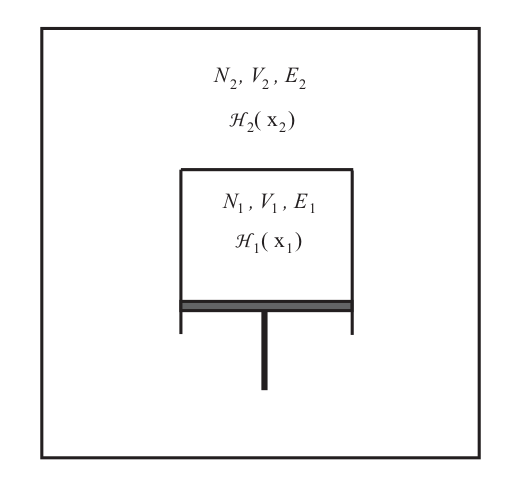
\includegraphics[scale=0.4]{isobar}
\label{fig:isobar}
\caption{Two systems in contact with a common thermal reservoir at temperature T. System
$1$ has $N_1$ particles in a volume $V_1$ ; system $2$ has $N_2$ particles in a volume $V_2$. Both $V_1$ and $V_2$ can vary.}
\end{figure}

\begin{multicols}{2}
	\begin{itemize}
		\item $E = E_1 + E_2\quad E_2\gg E_1$.
		\item $N = N_1 + N_2\quad N_2\gg N_1$.
		\item $V = V_1 + V_2\quad V_2\gg V_1$
		\item $\mathcal{H}(x) = \mathcal{H}_1(x_1) + \mathcal{H}_2(x_2)$.
	\end{itemize}
\end{multicols}


At fixed volumes $V_1$ and $V_2$:

$$Q(N, V, T) = C_N\int dx_1dx_2 e^{-\beta[\mathcal{H}_1(x_1) + \mathcal{H}_2(x_2)]} = g(N, N_1, N_2)C_{N_1}\int dx_1 e^{-\beta\mathcal{H}_1(x_1)}C_{N_2}\int dx_2 e^{-\beta\mathcal{H}_2(x_2)}$$

Which is the same expression for the micro canonical ensemble. $C_{N_1}$ and $C_{N_2}$ are the two constants that we would need to separate the system in two canonical ensemble with the same temperature $\beta$.

The partition function for the system is:

$$Q(N, V, T) \propto Q(N_1, V_1, T)Q(N_2, V_2, T)$$

But what happens if the volume is free to vary?

	\subsection{Phase space distribution}
	Combined system:

	$$f(x) = \frac{C_Ne^{-\beta\mathcal{H}(x)}}{Q(N, V, T)} = \frac{g(N, N_1, N_2)}{Q(N, V, T)}C_{N_1}e^{-\beta\mathcal{H}_1(x_1)}C_{N_2}e^{-\beta\mathcal{H}_2(x_2)}$$

We have to "wash out" the variables that describe the system $2$. So we need to integrate over the $x_2$ variables.

	$$f(x_1) = \frac{g(N, N_1, N_2)}{Q(N, V, T)}C_{N_1}e^{-\beta\mathcal{H}_1(x_1)}C_{N_2}\int dx_2 e^{-\beta\mathcal{H}_2(x_2)} = \frac{Q_2(N_2, V-V_1, T)}{Q(N, V, T)}g(N, N_1, N_2)C_{N_1}e^{-\beta\mathcal{H}_1(x_1)}$$

	The quantity $C_{N_2}\int dx_2 e^{-\beta\mathcal{H}_2(x_2)}$ is exactly the partition function for the system $2$, considered as a canonical ensemble, with a fixed number of particles and a given volume and temperature. Thus being equal to $Q_2$: let's focus on this quantity.

	First, the normalization is correct: $\int dV_1\int dx_1f(x_1, V_1) = 1$.

	Generally, we know that the partition function ($Q_2$ in this case) is equal to $e^{\beta[A]}$. So let's write this equation with the correct argument for the Helmholtz free energy.

	$$\frac{Q_2(N_2, V-V_1, T)}{Q(N, V, T)} = e^{-\beta[A(N-N_1, V-V_1, T) - A(N, V, T)]}$$

Through a Taylor expansion:

	$$A(N-N_1, V-V_1, T) = A(N, V, T)-N_1\frac{\partial A}{\partial N}|_{N_1 = 0, V_1 = 0} = A(N, V, T)-\mu N_1 + PV_1$$

	The phase-space distribution for variable $x_1$ is:

	$$f(x_1) = g(N, N_1, N-N_1) e^{\beta\mu N_1}e^{-\beta P V_1}C_{N_1}e^{-\beta\mathcal{H}_1(x_1)}\qquad I_{N_1} = \frac{1}{V_0N_1!h^{3N_1}}$$

	We define a quantity $\Delta(N, P, T)$ to be the integral of hte entire phase-space, including the volume, of the constant $I_N$. The phase-space distribution is simply $e^{-\beta(\mathcal{H}(x) + PV)}$, so basically the analogous distribution function of the canonical ensemble, but instead of having the energy in the Boltzmann factor we have the enthalpy.

	$$\Delta(N, P, T) = I_N\int_0^{\infty}dV\int dxe^{-\beta(\mathcal{H}(x) + PV)}\Rightarrow e^{\beta\mu N}\Delta(N, P, T) = 1$$

	Because of Euler (next chapter), the quantity $\mu N$ is exactly $G$:

	$$\Delta(N, P, T) = e^{-\beta\mu N} = e^{-\beta G(N, P, T)}$$

	Now we have an analogous relation: $e^{\beta A} \rightarrow e^{\beta G}$.

	$$\Delta(N, P, T) = \frac{1}{V_0N!h^{3N}}\int_0^{\infty}dVe^{-\beta PV}\int dxe^{-\beta\mathcal{H}(x)} = \frac{1}{V_0}\int_0^{\infty}dVe^{-\beta PV}Q(N, V, T)$$

	\subsubsection{Further proof}
	A further proof that this is indeed a "good" system is provided, starting this time from the Gibbs free energy.

	$$G = A + P\langle V \rangle = \langle E + PV\rangle - TS = \langle\mathcal{H}(x) + PV\rangle + T\frac{\partial G}{\partial T}$$

We can obtain the average $langle E + PV\rangle$ by performing the average over the phase-space distribution we just introduced. We need to integrate over the volume and all the coordinates. The quantity $(\mathcal{H}(x) + PV)$ (remember that $V$ now is a constant) must be weighted by the corresponding Boltzmann factor, which includes not only the hamiltonian but also $PV$.

	$$\langle E + PV\rangle = \frac{I_N\int_0^{\infty} dV\int dx(\mathcal{H}(x) + PV)e^{-\beta(\mathcal{H}(x)+PV)}}{I_N\int_0^{\infty}dV\int dxe^{-\beta(\mathcal{H}(x) + PV)}} = -\frac{1}{\Delta(N, P, T)}\frac{\partial \Delta(N, P, T)}{d\beta} = -\frac{\partial\ln\Delta(N, P, T)}{\partial \beta}$$


	$$G(N, P, \beta) = -\frac{\partial\ln\Delta(N, P, \beta)}{\partial\beta}-\beta\frac{\partial G}{\partial \beta}$$

	If we plug in the following solution: $G(N, P, \beta) = -\frac{1}{\beta}\ln\Delta(N, P, \beta)$ in the previous differential equation we get $0$.

	We now have all the means to describe the system.

	$$\langle V\rangle = \biggl(\frac{\partial G}{\partial P}\biggr)_{N, T}\qquad S = -\biggl(\frac{\partial G}{\partial T}\biggr)_{N, P}$$

	\subsection{Maxwell's square}

	Let's put everything into perspective.

	We have seen in the NPT enseble that we can obtain the average volume as the derivative wrt pressure of the Gibbs free energy, the entropy can be taken as the derivative wrt temperature (keeping fixed N and T).
	\begin{multicols}{2}
		\begin{itemize}
			\item $\langle V\rangle = \biggl(\frac{\partial G}{\partial P}\biggr)_{N, T}$.
			\item $S = -\biggl(\frac{\partial G}{\partial T}\biggr)_{N, P}$.
		\end{itemize}
	\end{multicols}

	We also found the following equation from the isobaric-isoenthalpic ensemble:

	\begin{multicols}{2}
		\begin{itemize}
			\item $T = \biggl(\frac{\partial H}{\partial S}\biggr)_{N, P}$.
			\item $\langle V\rangle = \biggl(\frac{\partial H}{\partial P}\biggr)_{N, S}$.
		\end{itemize}
	\end{multicols}

The following are coming from the microcanonical ensemble :
	\begin{multicols}{2}
		\begin{itemize}
			\item $T = =\biggl(\frac{\partial U}{\partial S}\biggr)_{N, V}$.
			\item $P = - \biggl(\frac{\partial U}{\partial V}\biggr)_{N, S}$.
		\end{itemize}
	\end{multicols}

And the canonical ensemble:
	\begin{multicols}{2}
		\begin{itemize}
			\item $P = -\biggl(\frac{\partial A}{\partial V}\biggr)_{N, T}$.
			\item $S = - \biggl(\frac{\partial A}{\partial T}\biggr)_{N, V}$.
		\end{itemize}
	\end{multicols}

	\begin{figure}[H]
		
\includegraphics[scale = 0.1]{maxwell_square}
		\centering
		\caption{Maxwell's square}
	\end{figure}


	\subsection{Pressure viral theorem}
	The internal pressure that was calculated by the estimator was a function of all the coordinates and all the momenta. The internal pressure $P^{int}$ would be the average of this estimator. We want this quantity to be equal to the external pressure for the equations to be valid.
	$$P^{(int)} =\langle\mathcal{P}(\vec{r}, \vec{p})\rangle = \biggl\langle\frac{1}{3V}\sum\limits_i\biggl[\frac{\vec{p}_i^2}{m_i} + \vec{F}_i\cdot\vec{r}_i\biggr]\biggr\rangle = kT\frac{\partial\ln Q}{\partial V}$$

To take average of this quantity for our new ensemble (NPT) we need to write down the partition function at the denominator and integrate over the volume.

	\begin{align*}
		\langle P^{(int)}\rangle &= \frac{1}{\Delta(N, P, T)}\int_0^{\infty}dVe^{-\beta PV}Q(N, V, T)\frac{kT}{Q}\frac{\partial Q}{\partial V} = \frac{kT}{\Delta(N, P, T)}\int_0^{\infty}dVe^{-\beta PV}\frac{\partial Q}{\partial V}=\\
														 &= \frac{kT}{\Delta(N, P, T)}e^{-\beta PV}Q(N, V, T)|_0^{\infty}-\frac{kT}{\Delta(N, P, T})\int_0^{\infty}dV\biggl(-\frac{P}{kT}\biggr)e^{-\beta PV}Q(N, V, T) = \\
														 &=\frac{P}{\Delta(N, P, T)}\int_0^{\infty}dVe^{-\beta PV}Q(N, V, T) = P
	\end{align*}

	Consider the integration by parts of the quantity $\frac{kT}{\Delta(N, P, T)}e^{-\beta PV}Q(N, V, T)|_0^{\infty}$: when the volume tends to infinity the exponential goes to zero; when instead the volume is zero the partition function is zero, because there are no states where $V=0$.
	We are left with only the second term and its integral is exactly $\Delta$.
	Again, the quantity $dVe^{-\beta PV}Q(N, V, T)$ is equal to $\Delta$ and we get the external pressure $P$.
	We demonstrated that if we take the average of the internal pressure over the NPT ensemble we obtain exactly the external pressure $P$, which is expected.
	 This also means that if we want to compare what we get in the simulation with the external pressure that we are fixing, we should calculate the internal pressure and then calculate the average over many simulations.

	 \paragraph{Take home message for the virial theorem: the volume-average internal pressure is equal to the external pressure}

	\subsection{Work virial theorem}
If we multiply the internal pressure for the volume (that changes):
	$$P^{(int)}V = kTV\frac{\partial \ln Q}{\partial V}$$

Then we obtain the same equations as before, but we need to include also the V:
	\begin{align*}
		\langle P^{(int)}V\rangle &= \frac{1}{\Delta(N, P, T)}\int_0^{\infty}dVe^{-\beta PV}Q(N, V, T)\frac{kTV}{Q}\frac{\partial Q}{\partial V} = \frac{kT}{\Delta(N, P, T)}\int_0^{\infty}dVe^{-\beta PV}V\frac{\partial Q}{\partial V} = \\
															&=\frac{kT}{\Delta(N, P, T)}e^{-\beta PV}VQ(N, V, T)|_{0}^{\infty}-\frac{kT}{\Delta(N, P, T)}\int_0^{\infty}dV\frac{\partial}{\partial V}(Ve^{-\beta PV})Q(N, V, T)=\\
															&= \frac{1}{\Delta(N, P, T)}\biggl[-kT\int_0^{\infty}dVe^{-\beta PV}Q(N, V, T) + P\int_0^{\infty}dV \, Ve^{-\beta PV}Q(N, V, T)\biggr]=\\
															&=-kT+P\langle V\rangle \Rightarrow \langle P^{(int)}V\rangle + kT = P\langle V\rangle
	\end{align*}

	The term $\int_0^{\infty}dV \, Ve^{-\beta PV}Q(N, V, T)$ is the average of the volume: the volume is multiplied by a weighting factor and divided by the partition function in the NPT ensemble.
	The work is equal to the average quantity $\langle P^{(int)}V\rangle$, plus $kT$.
	Now, $kT$ indicates that is equaiton is the analogous of the equipartition theorem, but there's an extra degree of freedom, the varying volume. This is the reason why an additional $kT is present$.
	To be fair, $kT$ is very small and it does not change much the final equation.


	 \paragraph{Take home message for the work virial theorem: There is an extra degree of freedom, that is the volume.}

	These theorems are particularly important, since the algorithms we will see later are all written for the isobaric-isoenthlapic ensemble, but we can go to easily by adding a thermostat.


\section{Andersen's Hamiltonian}
The best way to deal with the extra degree of freedom that (the volume) is to add it to the hamiltonian, as an extra variable, obviously with its own momentum.

This is the case of the Andersen's hamiltonian, defined as:

$$\mathcal{H}_A = \sum\limits_{i=1}^N\frac{V^{-\frac{2}{3}}\pi_i^2}{2m_i}+ U(V^\frac{1}{3}\vec{s}_1, \dots, V^{\frac{1}{3}}\vec{s}_N) + \frac{p_V^2}{2W} + PV\qquad W = (3N+1)kT\tau_b^2$$


We need to write down now Hamilton's equations, to obtain the time evolution for each of these coordinates:

\begin{itemize}
	\item $\dot{\vec{s}}_i = \frac{\partial \mathcal{H}_A}{\partial\pi_i} = \frac{V^{-\frac{2}{3}}\pi_i}{m_i}$.
	\item $\dot{\pi}_i = -\frac{\partial\mathcal{H}_A}{\partial\vec{s}_i} = -\frac{\partial U}{\partial (V^{\frac{1}{3}}\vec{s}_i)}V^{\frac{1}{3}}$.
	\item $\dot{V} = \frac{\partial\mathcal{H}_A}{\partial p_V}-\frac{p_V}{W}$.
	\item $\dot{p}_V = -\frac{\partial\mathcal{H}_A}{\partial V} = \frac{1}{3}V^{-\frac{5}{3}}\sum\limits_{i=1}^N\frac{\pi_i^2}{m_i}-\frac{1}{3}V^{-\frac{2}{3}}\sum\limits_{i=1}^N\frac{\partial U}{\partial(V^{\frac{1}{3}}\vec{s}_i)}\cdot\vec{s}_i-P$.
\end{itemize}

The derivative of $\dot{p}_V$ is slightly more complicated, since the dependence on $p$ is present on three terms.

Inverting the transformation (the same inversion we performed to go from original coordinates to the scaled coordinates):

$$s_i = V^{-\frac{1}{3}}\vec{r}_i\Rightarrow \dot{\vec{s}}_i = V^{-\frac{1}{3}}\dot{\vec{r}}_i-\frac{1}{3}V^{-\frac{4}{3}}\dot{V}\vec{r}_i$$


$$\pi_i = V^{\frac{1}{3}}\vec{p}_i \Rightarrow \dot{\pi}_i = V^{\frac{1}{3}}\dot{\vec{p}}_i + \frac{1}{3}V^{-\frac{2}{3}}\dot{V}\vec{p}_i$$


We need to substitute these equation to the ones we previously derived:

\begin{itemize}
	\item $\dot{\vec{s}}_i = \frac{\partial \mathcal{H}_A}{\partial\pi_i} = \frac{V^{-\frac{2}{3}}\pi_i}{m_i} \rightarrow \dot{r}_i = \frac{p_i}{m_i} + \frac{\dot{V}}{3V} r_i$
	\item $\dot{\pi}_i = -\frac{\partial\mathcal{H}_A}{\partial\vec{s}_i} = -\frac{\partial U}{\partial (V^{\frac{1}{3}}\vec{s}_i)}V^{\frac{1}{3}} \rightarrow \dot{p}_i = - \frac{\partial U}{\partial r_i} - \frac{\dot{V} }{3V} p_i$ .
	\item $\dot{V} = \frac{\partial\mathcal{H}_A}{\partial p_V}-\frac{p_V}{W} \rightarrow \dot{V} = \frac{p_V}{W}$.
	\item $\dot{p}_V = -\frac{\partial\mathcal{H}_A}{\partial V} = \frac{1}{3}V^{-\frac{5}{3}}\sum\limits_{i=1}^N\frac{\pi_i^2}{m_i}-\frac{1}{3}V^{-\frac{2}{3}}\sum\limits_{i=1}^N\frac{\partial U}{\partial(V^{\frac{1}{3}}\vec{s}_i)}\cdot\vec{s}_i-P \rightarrow \dot{p}_V = \frac{1}{3V} \sum^N_{i=1} [\frac{p^2_i}{m_i} - \frac{\partial U}{\partial r_i} r_i] -P$.
\end{itemize}

Notice how the new term $ \frac{\dot{V}}{3V}$ accounts for the compressibility of the variable, letting it \textit{inflating} and \textit{deflating}.

Also notice that the last quantity is exactly the internal pressure estimator. We have now a variation in the momentum, that is conjugate to the volume, whenever the internal pressure differs from the external one ($\dot{p} != 0$).

The compressibility is equal to $0$ (incompressible).
To calculate the compressibility we need to take the derivative of $\dot{r}$ wrt $r_i$, yielding a factor which is $\frac{\dot{V}}{3V}$ for each particle and every degree of freedom (three for each particle).

	\subsection{Andersen's equations}

	\begin{multicols}{2}
		\begin{itemize}
			\item $\dot{\vec{r}}_i = \frac{\vec{p}}{m_i} + \frac{\dot{V}}{3V}\vec{r}_i\Rightarrow\dot{\vec{r}}_i = \frac{\vec{p}_i}{m_i} + \frac{\dot{V}}{3V}\vec{r}_i$
			\item $\dot{\vec{p}}_i = -\frac{\partial U}{\partial\vec{r}_i} -\frac{\dot{V}}{3V}\vec{p}_i\Rightarrow \dot{\vec{p}}_i = -\frac{\partial U}{\partial\vec{r}_i}-\frac{\dot{V}}{3V}\vec{p}_i$.
			\item $\dot{V} = \frac{p_V}{W}\Rightarrow\dot{V} = \frac{p_V}{W}$.
			\item $\dot{p}_V = \frac{1}{3V}\sum\limits_{i=1}^N\biggl[\frac{\vec{p}_i^2}{m_i}-\frac{\partial U}{\partial\vec{r}_i}\cdot\vec{r}_i\biggr]-P\Rightarrow\dot{p}_V = \frac{1}{3V}\sum\limits_{i=1}^N\biggl[\frac{\vec{p}_i^2}{m_i}-\frac{\partial U}{\partial\vec{r}_i}\cdot\vec{r}_i\biggr]-P$.
		\end{itemize}
	\end{multicols}

	The conserved quantity:

	$$\mathcal{H}' = \sum\limits_{i=1}^N\frac{\vec{p}_i^2}{2m_i} + U(\vec{r}_1, \dots, \vec{r}_N) + \frac{p_V^2}{2W}+PV$$
	Notice how $\mathcal{H}'$ looks very similar to the enthalpy, aside from the kinetic energy part.
	As usual, when we work in a system that is not hamiltonian (we started from a different hamiltonian, $\mathcal{H}'$ does not give back Anderson's equations) we need to derive the partition function:

	$$\Omega_P = \int dp_V\int_0^{\infty}\int d^N\vec{p}\int_{\mathcal{D}(V)}d^N\vec{r}\delta\biggl(\\mathcal{H}(\vec{r},\vec{p}) + \frac{p_V^2}{2W}+PV-H\biggr)$$

	Virial theorem:

	$$\biggl\langle\frac{p_V^2}{2W}\biggr\rangle = k\frac{T}{2}\Rightarrow \mathcal{H}(\vec{r},\vec{p}) + PV\text{ is conserved}$$

	The pressure (the average) will be kept constant, as for the enthalpy.

\section{MTK algorithm (NPT)}
One of the best choices for thermostatting the system is the MTK algorithm, developed by Martyna-Tobias-Klein in 1994.
This algorithm introduces a new variable $\epsilon$:

$$\epsilon = \frac{1}{3}\ln\frac{V}{V_0}\Rightarrow\dot{\epsilon} = \frac{\dot{V}}{3V}=\frac{p_\epsilon}{W}$$

\begin{multicols}{2}
	\begin{itemize}
		\item $\dot{\vec{r}}_i = \frac{\vec{p}_i}{m_i} + \frac{p_\epsilon}{W}\vec{r}_i$.
		\item $\dot{\vec{p}}_i = -\frac{\partial U}{\partial\vec{r}_i} - \frac{p_\epsilon}{W}\vec{p}_i$.
		\item $\dot{V} = \frac{dVp_\epsilon}{W}$.
		\item $\dot{p}_\epsilon = dV(\mathcal{P}^{(int)}-P)$.
	\end{itemize}
\end{multicols}


Compressibility:

\begin{align*}
	\kappa & = \sum\limits_{i=1}^N\biggl[\frac{\partial}{\partial\vec{r}_i}\cdot\dot{\vec{r}}_i + \frac{\partial}{\partial\vec{p}_i}\cdot\dot{\vec{p}}_i\biggr] + \frac{\partial\dot{V}}{\partial V} + \frac{\partial\dot{p}_V}{\partial p_V} = \\
				 &= dN\frac{p_\epsilon}{W}-dN\frac{p_\epsilon}{W} = d\frac{p_\epsilon}{E} = \frac{\dot{V}}{V}
\end{align*}

To obtain incompressible equations that conserve $\mathcal{H}(\vec{r},\vec{p}) + PV + \frac{p_V^2}{2W}$ we need to apply some modifications:

$$\dot{\vec{p}}_i = -\frac{\partial U}{\partial\vec{r}_i} - \biggl(1+\frac{d}{N_F}\biggr)\frac{p_\epsilon}{W}\vec{p}_i\qquad \dot{p}_\epsilon = dV(\mathcal{P}^{(int)}-P) + \frac{d}{N_f}\sum\limits_{i=1}^N\frac{\vec{p}_i^2}{m_i}$$

With $F$ being the number of degrees of freedom of the system.

	\subsection{Langevin piston}
	In many programs and applications, we will use the Langevin thermostat.
	The only difference from the Andersen's equations is the last one, with a friction acting on the volume and a last term representing a random force (or "kick").

	\begin{itemize}
		\item $\dot{\vec{r}}_i = \frac{\vec{p}_i}{m_i} + \frac{\dot{V}}{3V}\vec{r}_i$.
		\item $\dot{\vec{p}}_i = -\frac{\partial U}{\partial\vec{r}_i}-\frac{\dot{V}}{3V}\vec{p}_i$.
		\item $\dot{V} = \frac{p_V}{W}$.
		\item $\dot{p}_V = \frac{1}{3V}\sum\limits_{i=1}^N\biggl[\frac{\vec{p}_i^2}{m_i}-\frac{\partial U}{\partial\vec{r}_i}\cdot\vec{r}_i\biggr]-P-\gamma\dot{V}+R(t)$.
	\end{itemize}

	$$\langle R(0)R(t)\rangle = \frac{2\gamma kT}{W}\delta(t)$$

	The Langevin piston is mostly preferred as a barostat (it will not be thoroughly described though, as its equations are more complicated).

\section{Summary}
\begin{itemize}
\item We constructed the formalism of the isobaric ensembles, starting by performing the Legendre transform of the micro canonical ensemble to obtain the isobaric-isoenthalpic esnable; then the same reasoning was applied to the canonical ensemble to obtain the isobaric - isothermal (NPT) ensemble.
\item We demonstrated that the steps and the reasoning to modify the equations of the micorcanonical ensemble to go to the canonical ensemble, apply pretty much in the same way also for isobaric-isoenthalpic for the NPT.
\item In the NPT ensemble we can calculate everything like a canonical ensemble, however the volume is now a variable.
\item the pressure virial theorem, important for molecular simulations, and work virial theorem, useful for the derivation of Andersen's hamiltonian, were introduced.
\end{itemize}

  % \graphicspath{{chapters/13/images/}}
\chapter{The grand canonical ensemble}

\section{Introduction}
The Gran Canonical (GC) ensemble comes in handy when the number of molecules cannot be kept fixed during the simulation.
This is one of the main differences between MD and MC approaches: it is not possible to perform MD simulations with varying number of molecules.

	\subsection{Euler's theorem}
	Homogeneous function $f(x_1, \dots, x_N)$ of degree $n$ in $x_1, \dots, x_k$:

	$$f(\lambda x_1, \dots, \lambda x_k, x_{k+1}, \dots, x_N) = \lambda^n f(x_1, \dots, x_k, \dots, x_N)$$

	This property states that if each variable $(x_1, ... x_k)$ is increased by a certain value $\lambda$, then the net result is that the value of the function is increased by a factor $\lambda^n$.
	An example of this property can be showed by the homogeneous function $f(x) = x^2$, $f(x, y, z) = xy^2+z^3$.
	The degree is $3$ and each variable $(x, y, z)$ is increased by a factor $\lambda$.
	Taking the derivative:

	$$\frac{d}{d\lambda} f(\lambda x_1, \dots, \lambda x_k, \dots, x_N) = n\lambda^{n-1}f(x_1, \dots, x_k,\dots, x_N)$$

	If the partial derivative is calculated with respect to each variable and then the derivative of the variable itself with respect to $\lambda$ is obtained:

	$$\frac{d}{d\lambda}f(\lambda x_1, \dots, \lambda x_k, \dots, x_N) = \sum\limits_{i=1}^k\frac{\partial f(x_1, \dots, x_k, \dots, x_N)}{\partial x_i}x_i$$

	Meaning that the two quantities are equal and the following property (for an homogeneous function) can be obtained:

	$$\lambda = 1 \Rightarrow \sum\limits_{i=1}^k\frac{\partial f}{\partial x_i}x_i = nf(x_1, \dots, x_N)$$

	\subsection{Applications}
	Euler's theorem has important consequences in thermodynamics, as it means that all of the thermodynamics function can be expressed in terms of other parameters, and it is valid for every substance.
	Applying Euler's theorem to the internal energy $U$:

	$$U(\lambda N, \lambda V, \lambda S) = \lambda U(N, V, S)\Rightarrow U(N, V, S) = \frac{\partial U}{\partial N}N + \frac{\partial U}{\partial V}V_\frac{\partial U}{\partial S}S = \mu N - PV + TS$$

	Each of the above partial derivatives are easily calculated through Maxwell square.
	Applying the theorem to Helmholtz free energy:

	$$A(\lambda N, \lambda V, T) = \lambda A(N, V, T) \Rightarrow A(N, V, T) = \frac{\partial A}{\partial N}N + \frac{\partial A}{\partial V}V = \mu N - PV$$

	The difference here is that the extensive quantities are $N$ and $V$, while $T$ is an intensive quantity.
	The function is not homogeneous in $T$, e.g. if T is increased by a factor $\lambda$ the whole function is not increased.
	Applying it now to the enthalpy:

	$$H(\lambda N, \lambda S, P) = \lambda H(N, S, P)\Rightarrow H(N, S, P) = \frac{\partial H}{\partial N}N+\frac{\partial H}{\partial N}N+\frac{\partial H}{\partial S}S = \mu N+TS$$

	Like for $A$, the enthalpy is a homogeneous function for two of its variables, but not for $P$.
	Finally, considering Gibbs free energy:

	$$G(\lambda N, P, T) = \lambda G(N, P, T)\Rightarrow G(N, P, T) = \frac{\partial G}{\partial N}N= \mu N$$

	It has only one dependency on an extensive quantity: the number of particles.
	The fact that the chemical potential $\mu$ is exactly $G$ divided by $N$, as demonstrated in the previous chapter can be obtained.

	\subsection{Legendre transform of A}
	Applying the same reasoning that was applied to the isobaric ensembles:

	$$\tilde{f}(s) = f(x(s))-sx(s)\qquad s = f'(x)$$

	The Legendre transform will not be applied in terms of volume, but instead in terms of its derivative with respect to the number of molecules:

	\begin{align*}
		\tilde{A}\biggl(\frac{\partial A}{\partial N}, V, T\biggr) &= A(N(\mu), V, T)-\biggl(\frac{\partial A}{\partial N}\biggr)_{N, V}N\biggl(\frac{\partial A}{\partial N}, V, T\biggr) = \\
																															 &=A(N(\mu), V, T) - \mu N = \mu N - PV - \mu N = -PV
	\end{align*}

	From the results obtained before, the result of the Legendre transform is simply $-PV$.
	Now the infinitesimal variation of the transformed $A$ has to be computed:

	$$d\tilde{A} = dA - Nd \mu -\mu dN = -PdV - SdT + \mu dN -Nd\mu - \mu dN$$

	$$d\tilde{A} = -PdV - SdT - Nd\mu$$

	$$\tilde{A}(\mu, \lambda V, T) = \lambda\tilde{A}(\mu, V, T)\Rightarrow \tilde{A}(\mu, V, T) = \frac{\partial \tilde{A}}{\partial V}V = -PV$$

	Notice that $\tilde{A}$ depends on only one extensive variable ($V$), so Euler's theorem can be applied again.


\section{Grand canonical ensemble}
As for the previous ensembles, the analysis starts from the definition of the main variables of the equations and in figure \ref{fig:grand} the two systems are depicted.

\begin{figure}[H]
\center
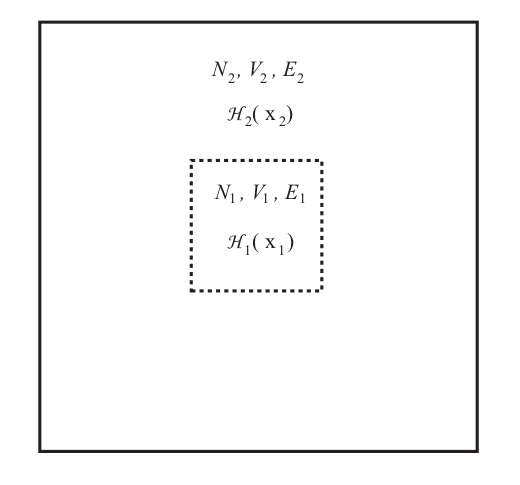
\includegraphics[scale=0.5]{grand.png}
\caption{Two systems in contact with a common thermal reservoir at temperature $T$. System $1$ has $N_1$ particles in a volume $V_1$ ; system 2 has $N_2$ particles in a volume $V_2$. The dashed lines indicate that systems $1$ and $2$ can exchange particles.}
\label{fig:grand}
\end{figure}

\begin{multicols}{2}
	\begin{itemize}
		\item $E = E_1 + E_2\quad E_2\gg E_1$.
		\item $N = N_1 + N_2\quad N_2\gg N_1$.
		\item $V = V_1 + V_2\quad V_2\gg V_1$.
		\item $\mathcal{H}(x, N) = \mathcal{H}_1(x_1, N_1) + \mathcal{H}_2(x_2, N_2)$.
	\end{itemize}
\end{multicols}

The partition function is the same as a canonical ensemble when the exchange of molecules between the two systems is stopped:

$$Q(N, V, T) = \frac{1}{N!h^{3N}}\int dx_1\int dx_2e^{-\beta[\mathcal{H}_1(x_1) + \mathcal{H}_2(x_2)]}$$

At fixed $N_1$ and $N_2$, not allowing any other exchange of particles, then the partition function is:

$$Q(N, V, T) = \frac{N_1!N_2!}{N!}\frac{1}{N_1!h^{3N_1}}\int dx_1 e^{-\beta\mathcal{H}_1(x_1)}\frac{1}{N_2!h^{3N_2}}\int dx_2^{-\beta\mathcal{H}_2(x_2)} = \frac{N_1!N_2!}{N!}Q_1(N_1, V_1, T)Q_2(N_2, V_2, T)$$

With a varying particle numbers:

$$Q(N, V, T) = \sum\limits_{N_1=0}^Ng(N_1, N-N_1)\frac{N_1!(N-N_1)!}{N!}Q_1(N_1, V_1, T)Q_2(N-N_1, V-V_1, T)$$

The factor $g$ is a combinatorial (or degeneracy) factor, and indicates in how many ways the particles can be divided in one box and the other, or in how many ways there are $N_1$ particles in system $1$ and $N_2$ particles in system $2$.
It is defined as:
$$g(N_1, N-N_1) = \frac{N!}{N_1!(N-N_1)!}$$

\begin{multicols}{3}
	\begin{itemize}
		\item $N_1 = 0\Rightarrow g(0, N) = 1$.
		\item $N_1 = 1\Rightarrow g(1, N-1) = N$.
		\item $N_1 = 2\Rightarrow g(2, N-2) = \frac{N(N-1)}{2}$.
	\end{itemize}
\end{multicols}

So the total partition function is defined as:

$$Q(N, V, T) = \sum\limits_{N_1=0}^NQ_1(N_1, V_1, T)Q_2(N-N_1, V-V_1, T)$$

However for the full system, considered as a canonical ensemble, the partition function is known:

$$f(x, N) = \frac{e^{-\beta\mathcal{H}(x, N)}}{N!h^{3N}Q(N, V, T)}\Rightarrow dxf(x, N) = 1$$

And the phase space distribution of system $1$: $\sum\limits_{N_1=0}^{N}\int dx_1f(x_1, N_1) = 1$.

\begin{align*}
	f(x_1, N_1) &=\biggl(\frac{e^{-\beta\mathcal{H}_1(x_1, N_1)}}{Q(N, V, T)N_1!h^{3N_1}}\biggr)\frac{1}{(N-N_1)!h^{3(N-N_1)}}\int dx_2e^{-\beta\mathcal{H}_2(x_2, N-N_1)} = \\
							&= \frac{Q_2(N-N_1, V-V_1, T)}{Q(N, V, T)}\frac{1}{N_1!h^{3N_1}}e^{-\beta\mathcal{H}_1(x_1, N_1)}
\end{align*}

$$\frac{Q_2(N-N_1, V-V_1, T)}{Q(N, V, T)} = e^{-\beta[A(N-N_1, V-V_1, T) - A(N, V, T)]}$$

$$A(N-N_1, V-V_1, T)\approx A(N, V, T) -\frac{\partial A}{\partial N}N_1-\frac{\partial A}{\partial V}V_1 = A(N, V, T)-\mu N_1 + PV_1$$


	\subsection{Grand partition function}

	The phase-space distribution is:

	$$f(x_1, N_1) = \frac{1}{N_1!h^{3N_1}}e^{\beta\mu N_1}e^{-\beta PV_1}e^{\beta\mathcal{H}_1(x_1, N_1)}$$

	In the equation there's no dependence on $N_2$ and the subscript $1$ can be dropped :

	$$f(x, N) = \frac{1}{N!h^{3N}}e^{\beta\mu N}e^{-\beta PV}e^{\beta\mathcal{H}(x, N)}$$

	Taking exactly the normalization condition:

	$$\sum\limits_{N=0}^{\infty}\int dxf(x, N) = \sum\limits_{N=0}^{\infty}e^{-\beta PV}\frac{1}{N!h^{3N}}e^{\beta\mu N}\int dxe^{-\beta\mathcal{H}(x, N)} = 1$$

	The same function as in the canonical ensemble is obtained, and the partition function of the grand-canonical ensemble is $e^{\beta PV}$, as supposed by Euler's theorem.

	$$\sum\limits_{N+0}^{\infty}\frac{1}{N!h^{eN }}e^{\beta\mu N}\int dxe^{-\beta\mathcal{H}(x, N)} = e^{\beta PV}$$

	Now the equation of state of the system can be written:

	$$\mathcal{E}(\mu, V, T) = \sum\limits_{N=0}^{\infty}e^{\beta\mu N}\frac{1}{N!h^{3N}}\int dxe^{-\beta\mathcal{H}(x, N)} = \sum\limits_{N=0}^{\infty}e^{\beta\mu N}Q(N, V, T) = e^{\beta PV}$$

	$$\frac{PV}{kT} = \ln\mathcal{E}(\mu, V, T)$$

	Moreover the average of the particles can be computed:

	$$\langle N\rangle = \frac{1}{\mathcal{E}(\mu, V, T)}\sum\limits_{N=0}Ne^{\beta\mu N}Q(N, V, T) = kT\biggl(\frac{\partial}{\partial\mu}\ln\mathcal{E}(\mu, V, T)\biggr)_{V, T}$$

	Including the fugacity:

	$$z = e^{\beta\mu}$$

	The grand canonical partition function can be written down in an easier way to remember:

	$$\mathcal{E}(z, V, T) = \sum\limits_{N=0}^{\infty}z^NQ(N, V, T)$$

	This time it is not even necessary to write down the derivatives, as the equation of state simply derives from its definition.
	However, the above equation is not very easy to deal with, as it is a function of the chemical potential of the fugacity, the volume and the temperature, and it is not the usual way in which the equation of state is written.
	The derivative of $z$ with respect to $\mu$ returns the average number of molecules.

	$$\frac{\partial}{\partial\mu} = \frac{\partial z}{\partial\mu}\frac{\partial}{\partial z} = \beta z\frac{\partial}{\partial z}\Rightarrow\langle N\rangle = z\frac{\partial}{\partial z}\ln\mathcal{E}(z, V, T)$$

	The quantity $\langle N\rangle$ is the relation between the chemical potential (or grand-canonical partition function) and the number of molecules.

	\subsection{Ideal gas}
	Applying the grand canonical equation to an ideal gas, the canonical partition function will be:

	$$Q(N, V, T) = \frac{1}{N!h^{3N}}V^N\biggl[\int dp \, e^{-\beta\frac{p^2}{2m}}\biggr]^{3N} = \frac{1}{N!}\biggl[V\biggl(\frac{2\pi m}{\beta h^2}\biggr)^{\frac{3}{2}}\biggr]^{N} = \frac{1}{N!}\biggl(\frac{V}{\lambda^3}\biggr)^N$$

	The term $(\frac{2\pi m}{\beta h^2}\biggr)^{\frac{3}{2}}$ has the dimension of a length to the power of $-3$, and it is called the \textbf{thermal wave length}, and is is indicated with $\lambda$.

	Performing the sum of the series to obtain the grand canonical partition function:

	$$\mathcal{E}(z, V, T) = \sum\limits_{N=0}^{\infty}z^N\frac{1}{N!}\biggl(\frac{V}{\lambda^3}\biggr)^{N} = \sum\limits_{N=0}^{\infty}\frac{1}{N!}\biggl(\frac{zV}{\lambda^3}\biggr)^{N} = e^{\frac{zV}{\lambda^3}}$$

	Notice that also this time it is written in terms of the fugacity.
	Again, this form of the equation is hard to work with, so the average of the number of particles can be computed by taking the logarithm of the partition function and multiplying it for the derivative of the fugacity:

	$$\langle N\rangle = z\frac{\partial}{\partial z}\ln\mathcal{E}(z, V, T) = V\frac{z}{\lambda^3}\Rightarrow z = \frac{\langle N\rangle\lambda^3}{V}$$

	Meaning that the equation of state can be written as:

	$$\frac{PV}{kT} = \ln\mathcal{E}(z, V, T) = \frac{V_z}{\lambda^3}= \langle N\rangle$$

	It is easy to recognize the usual equation of state for an ideal gas, proving that this procedure works, as it yields the exact result for the ideal gas.

\section{Particle number fluctuations}
The grand canonical ensembles are extremely important in statistical mechanics, as they allow for easier calculations with respect to the canoncial or microcanonical ensembles.
The fact that the GC ensemble provides for a sum over a series makes the calculations easier, specifically in quantum statistical mechanics.
However, when in the GC ensemble, the net thermodynamics should not change.
In other words, the GC ensemble should be completely equivalent to the canonical one, in the sense that the thermodyanmics results obtained must be the same.
The difference between the two is the number of particles.
The fluctuations in the particle number has to be quantified: if they're too big, we could run into problems.
The particle number fluctuations are defined as:

$$\Delta N = \sqrt{\langle N^2\rangle-\langle N\rangle^2}$$

Defining them in terms of thermodynamics derivatives:

\begin{align*}
	z\frac{\partial}{\partial z}z\frac{\partial}{\partial z}\ln\mathcal{E}(z, V, T) &= z\frac{\partial}{\partial z}\frac{1}{\mathcal{E}}z\frac{\partial}{\partial z}\sum\limits_{N=0}^{\infty}z^NQ(N, V, T) = z\frac{\partial}{\partial z}\frac{1}{\mathcal{E}}\sum\limits_{N=0}^{\infty}Nz^N Q(N, V, T)=\\
																																									&=\frac{1}{\mathcal{E}}\sum\limits_{N=0}^{\infty}N^2z^NQ(N, V, T)-\frac{1}{\mathcal{E}^2}\biggl[\sum\limits_{N=0}^{\infty}Nz^NQ(N, V, T)\biggr]^2 = \langle N^2\rangle - \langle N\rangle^2
\end{align*}

The double derivative $z\frac{\partial}{\partial z}z\frac{\partial}{\partial z}$ is exactly equal to the average number of particles.
By the definition of fugacity:

$$kT\frac{\partial}{\partial\mu} = z\frac{\partial}{\partial z}\Rightarrow\Delta N^2 = (kT)^2\frac{\partial^2}{\partial\mu^2}\ln\mathcal{E}(\mu, V, T) = (kT)^2\frac{\partial^2}{\partial\mu^2}\frac{PV}{kT} = kTV\frac{\partial^2 P}{\partial\mu^2}$$

The result obtained is:

$$\Delta N^2 = kTV\frac{\partial^2 P}{\partial \mu^2}$$

But in order to get to something measurable other calculations have to be performed.
First of all, considering an "intensive Helmholtz free energy", this can be computed by dividing from the extensive Helmholtz free energy the number of particles and expressing it with intensive quantities:

$$a(v, T) = \frac{1}{N}A\biggl(N, \frac{V}{N}, T\biggr) \Rightarrow \mu = \frac{\partial A}{\partial N} = a(v, T) + N\frac{\partial a}{\partial v}{\partial v}{\partial N} = a(v, T) - V\frac{\partial a}{\partial v}$$

Where $v$ is the specific volume.
The pressure can be expressed in terms of the intensive Helmholtz:

$$P = -\biggl(\frac{\partial A}{\partial V}\biggr)_{N, T} = -N\frac{\partial a}{\partial v}\frac{\partial v}{\partial V} = -\frac{\partial a}{\partial v}\qquad\frac{\partial P}{\partial\mu} = \frac{\partial P}{\partial  v}{\partial v}{\partial\mu} = -\frac{\partial^2 a}{\partial v^2}\frac{\partial v}{\partial \mu}$$

Taking the derivative of the chemical potential with respect to the specific volume:

$$\frac{\partial\mu}{\partial v} = \frac{\partial a}{\partial v}-\frac{\partial a}{\partial v} - v \frac{\partial^2a}{\partial v^2}\Rightarrow \frac{\partial P}{\partial\mu} = \frac{1}{v}$$

Moreover, considering the second derivative:

$$\frac{\partial^2P}{\partial\mu^2} = -\frac{1}{v^2}\frac{\partial v}{\partial\mu} = \frac{1}{v^2}\biggl(v\frac{\partial^2 a}{\partial v^2}\biggr)^{-1} = -\frac{1}{v^3\frac{\partial P}{\partial v}}$$

$$\Delta N^2 = kTV\frac{\partial^2 P}{\partial\mu^2}\qquad\qquad\frac{\partial^2 P}{\partial\mu^2} = -\frac{1}{v^3\frac{\partial P}{\partial v}}$$

Solving all the terms the thermal compressibility $\kappa_T$ is obtained, a measurable quantity:

$$\kappa_T = -\frac{1}{V}\frac{\partial V}{\partial P} = -\frac{1}{v}\frac{\partial v}{\partial P} = -\frac{1}{v\frac{\partial P}{\partial v}}\Rightarrow\Delta N^2 = \frac{kTV}{v^2}\kappa_T = \frac{\langle N\rangle kT}{v}\kappa_T$$

The term $ -\frac{1}{V}$ is added because when pressure is applied, the volume is expected to decrease.
This thermal compressibility determines how much the system is compressible with respect to pressure.
The fluctuation needs to be compared to the quantity of interest, obtaining the relative fluctuation:

$$\frac{\Delta N}{\langle N\rangle} = \sqrt{\frac{kT}{v\langle N\rangle}\kappa_T}\sim\frac{1}{\sqrt{\langle N\rangle}}$$

If the average number of particles is "high", which it usually is, being in the thermodynamic limit, then the fluctuation is negligible.
Meaning that every calculation performed in the GC ensemble is equal to the canonical one.
However, $k_T$ is not always a finite number, in particular during a phase transition, in which the thermal compressibility can be quite high.
In such a case, since the particles are moving from one phase to another, the only usable ensemble is one that takes into account the fact that the number of particles is not constant: the grand canonical ensemble.

  % \graphicspath{{chapters/14/images/}}
\chapter{Quantifying uncertainties and sampling quality}

\section{Introduction}
Dealing with huge system and dealing with a huge amount of data is not sufficient to interpret the biological relevance of a molecular definition.
There is a need to perform thoughtful analysis on the obtained data.
Data interpretation is a fundamental step to asses the validity of a simulation.
The methods presented in this chapter will be useful also when dealing with Monte Carlo simulations, although the simulation is more difficult to interpret as time becomes moves.

	\subsection{Key definitions}

		\subsubsection{Expectation value}
		The Expectation value is defined as:

		$$\langle x\rangle = \int xP(x)dx = \sum\limits_jx_jP(x_j)$$

		In the case of molecular dynamics simulations time will be discretized, so the probability distribution will be discretized.

		\subsubsection{Estimate of expectation value}
		The estimate of the expectation value, or arithmetic mean is computed as:

		$$\bar{x} = \frac{1}{n}\sum\limits_{j=1}^nx_j$$

		\subsubsection{Variance}
		The variance is computed as:

		$$\sigma^2_x = \int dxP(x)(x-\langle x\rangle)^2 = \sum\limits_{j}P(x_j)\bigl(x_j-\langle x\rangle\bigr)^2$$

		\subsubsection{Standard deviation}
		The standard deviation is $\sigma_x$ and its estimate is the experimental standard deviation:

		$$s(x) = \sqrt{\frac{\sum\limits_{j=1}^n(x_j-\bar{x})^2}{n-1}}$$

		The estimates are necessary in molecular dynamics as the probability distribution is not known.

		\subsubsection{Linear correlation}
		Two variables are defined as linearly uncorrelated observables:

		$$\bigl\langle(x-\langle x\rangle)(y-\langle y\rangle)\bigr\rangle = 0$$

		Linear uncorrelation does not imply independent variables.

		\subsubsection{Experimental standard deviation}
		The experimental standard deviation of the mean is computed as:

		$$s(\bar{x}) = \frac{s(x)}{\sqrt{n}}$$

		If all the $x_j$ are assumed to be linearly uncorrelated, this is used to estimate error in computer simulations.

		\subsubsection{Correlation time}
		The correlation time $\tau$ is the longest separation time $\Delta t$ over which $x(t)$ and $x(t + \Delta t)$ remain linearly correlated.
		This is important as only data that are separated more than the correlation time are linearly uncorrelated and can be used when computing the standard deviation of mean.
		If they would be included the standard deviation would be underestimated.

		\subsubsection{Two sided confidence interval}
		Once the standard deviation is computed the two-sided confidence interval can be obtained: $\langle x\rangle = \bar{x} \pm U$ with $U = ks(\bar{x})$ and $k$ the coverage factor for a given level of confidence $p$ expressed in percentage.
		Usually $k=2$ to obtain a level of confidence about $95\%$, so that the expectation value is expected with $95\%$ probability to lie in the interval.
		This is the ideal situation, but there is no certainty that the molecular simulation will explore the entirety of the phase-space compatible with the macroscopic conditions.

	\subsection{Time scales}
	Before starting a simulation the time scale of the process of interest has to be estimated.
	For instance, looking at protein folding, obtained through experimental measure, the time scale could change from microseconds to minutes depending on the dimension of the protein.
	The latter case cannot be explored with a standard molecular simulation, so a coarse-grained model or other methods should be used to accelerate the dynamics (using approximations out of control, biasing the dynamics).

	\begin{figure}[H]
		\centering
		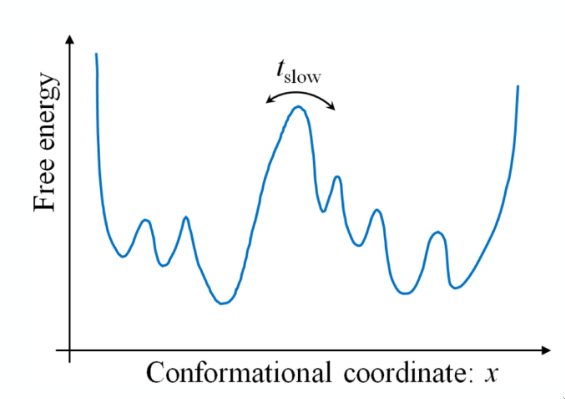
\includegraphics[scale = 0.4]{time-scales}
		\caption{Time scales}
		\label{fig:time-scales}
	\end{figure}

	Figure \ref{fig:time-scales} depicts a free energy profile.
	Usually when starting a simulation the starting point is a minimum.
	Sampling the simulation for a long time a transition to other minima could be observed, but these processes that happen to processes that happen on a faster time-scale with respect to processes that need to surpass a higher energy barrier.
	The time-scale of the transition depends exponentially on the height of the transition, so the higher the barrier the longer the time to observe the transition.
	Whenever a simulation is started an estimate of the slowest time scale involved in the process need to be understood.



\section{Equilibration}
When performing a simulation it is fundamental to consider if the simulation is equilibrated enough, so if the system has equilibrated after the simulation.
This is very difficult to understand, but it is easy to tell if a system is non-equilibrated.
Some of the variables that can be checked to see for non-equilibration are scalar values:

\begin{multicols}{2}
	\begin{itemize}
		\item System size which depends on the ensemble: in the case of NPT it is important.
			If it is equilibrated the volume would fluctuate around an average.
		\item Membrane area for membrane proteins: when simulating a protein at the beginning the membrane adapt to the protein and after a while equilibration is reached and area per lipid does not change and so does total membrane area.
		\item Potential energy or total energy, this is expected to fluctuate around an average value.
			At the beginning it varies due to temperature or initial configuration before reaching an average, so it as equilibrated in a local minimum of an average.
		\item Temperature in the NVE ensemble, so temperature will be constant when the system is at equilibrium.
		\item Density of simulated molecules in the NPT ensemble.
		\item Pressure, not recommended because in pressure there are huge variation because it depends on the Virial, so the average value will be $1 atm$, but the fluctuation will be huge.
		\item Radius of gyration is an overall information on the protein structure.
			There is the possibility to reach the same value in different conformation, a problem that applies to other overall distance measures.
			Even if there are conformation with the same value of gyration they could be different.
			If the radius of gyration is constantly increasing or decreasing the simulation has not equilibrated yet.
		\item Configurational distance measures like RNMS, all-to-all RMSD map.
			The discussion for radius of gyration holds for this measures.
			Considering RMSD:

			$$RMSD(\vec{r}, \vec{s}) = \sqrt{\frac{1}{N}\sum\limits_{i=1}^N|\vec{r}_i-\vec{s}_i|^2}$$

			This will reach a constant value with some fluctuation.
			The all-to-all RMSD map checks the RMSD for all the conformation present in the molecular dynamics simulation, obtaining a matrix of distances that can be plotted as in \ref{all-to-all-rmsd}.
	\end{itemize}
\end{multicols}

\begin{multicols}{2}

	\begin{figure}[H]
		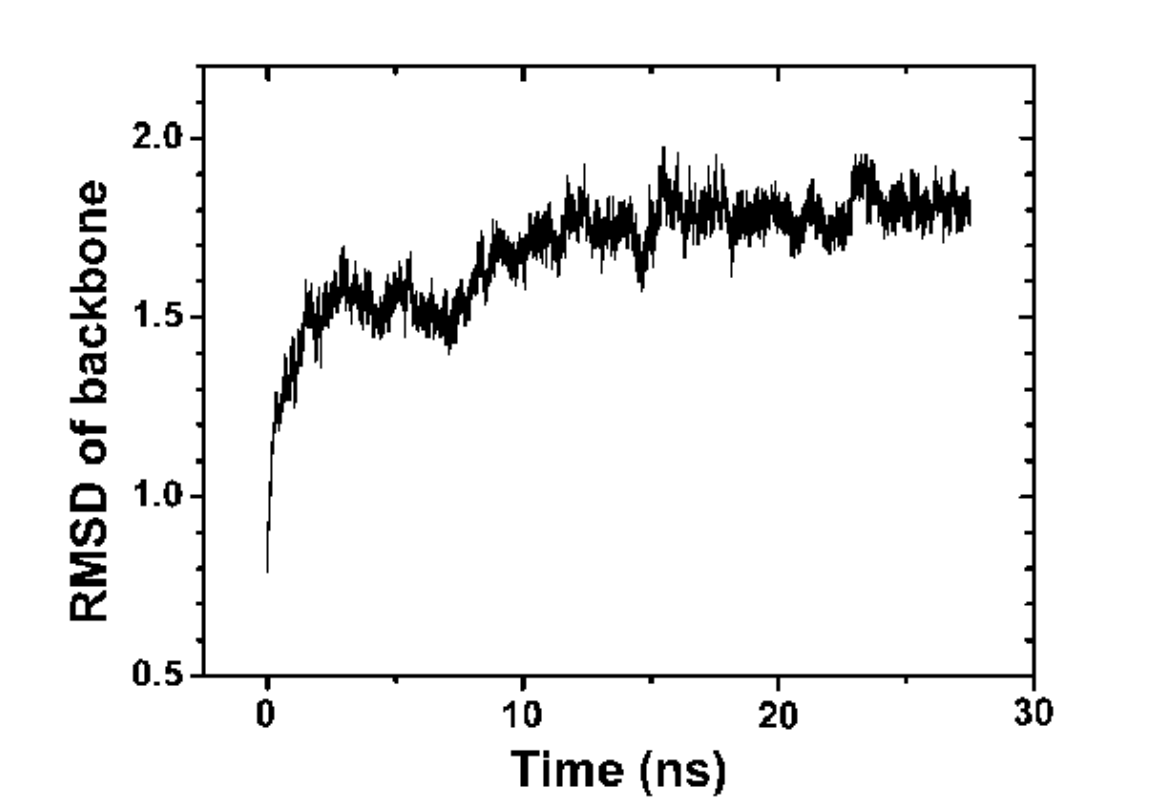
\includegraphics[width = 0.45\textwidth]{rmsd}
		\caption{RMSD}
		\label{fig:rmsd}
	\end{figure}

	\columnbreak

	\begin{figure}[H]
		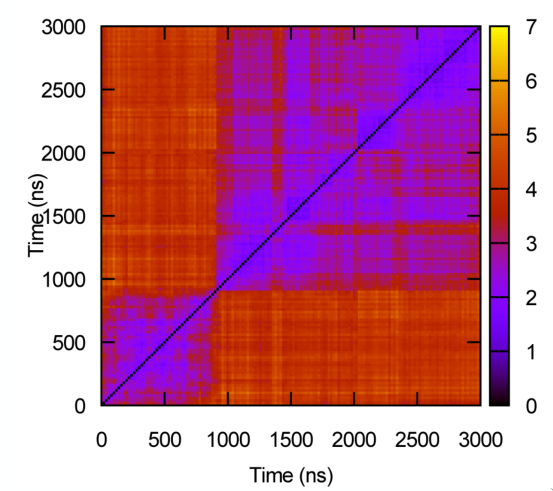
\includegraphics[width = 0.45\textwidth]{all-to-all-rmsd}
		\caption{All-to-all RMSD map, in blue low values and in red high value}
		\label{fig:all-to-all-rmsd}
	\end{figure}

\end{multicols}

It is very difficult to interpret data from \ref{fig:rmsd}, but it is easier in \ref{fig:all-to-all-rmsd}.
Looking at the latter two conformations can be seen, where there are the basins.
It can be seen how once the protein exits from the lower basin it does not come back and goes into the other.
Moreover in the bigger basis different conformation can be seen that are easily traversed.
This two basin are expected with starting with crystal's coordinate the first is the local basin corresponding to the crystal structure, which can be biased.

	\subsection{Qualitative behaviour}

	\begin{figure}[H]
		\centering
		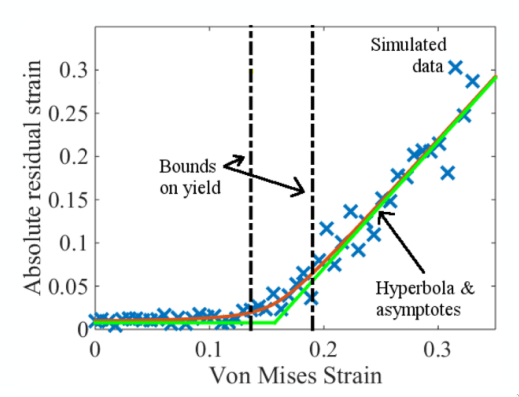
\includegraphics[scale=0.5]{qualitative-behaviour}
		\caption{Qualitative behaviour}
		\label{fig:qualitative-behaviour}
	\end{figure}

	Knowing some qualitative features of the simulation can allow for a more constructive analysis of the data.
	Looking at \ref{fig:qualitative-behaviour} a simulation of a material is considered.
	In this case an expected behaviour is seen and then the simulated data is fitted into a known function, so in this case the expected behaviour is being reproduced, meaning that the simulation has provided good results.

	\subsection{Independent simulations}
	In principle a set of independent simulations should be run.
	Most of the time running independent simulation is not a good choice in the case of protein.
	This is because all the independent simulation are independent only in the velocities: the coordinates are the same not considering the solvent.
	This is very computational expensive, so a more efficient way would be to run long simulation starting from equilibrating structure and randomizing the velocities.

		\subsubsection{Autocorrelation analysis}
		Another method is to start from a single simulation and perform an autocorrelation analysis, to asses whether two snapshots of the simulation are independent.
		To do so the autocorrelation of two quantities like RMSD is computed:

		$$C(x_k, x_{k+j}) \equiv\frac{\bar{(x_k-\bar{x})(x_{k+j}-\bar{x})}}{s^2(x)}\Rightarrow C_j$$

		Where:

		\begin{multicols}{2}
			\begin{itemize}
				\item $x_c$ is data point at time $c$.
				\item $\bar{x}$ is the arithmetic mean.
			\end{itemize}
		\end{multicols}

		This would be done for all the $k$ values and if it does not depend by $k$ but only on $j$ the property has been equilibrated.
		If the function depends on $k$ the simulation has equilibrated.

		\subsubsection{Combined clustering}
		Combined clustering as in \ref{fig:independent_simulation}.
		In combined clustering a measure of the distance of the conformation.
		Then using one clustering algorithm the conformations will be clustered.
		There will be a number of cluster.
		Assume doing so for two independent simulations, or for two part of a long simulation, called in \ref{fig:independent_simulation} $1$ and $2$.
		Then for each of this two simulation the time the simulation spent in one cluster is computed for each cluster.
		This is plotted in the data.
		If the point are off-diagonal the trajectories are not the same so the system has not equilibrated.

		\begin{figure}[H]
			\centering
			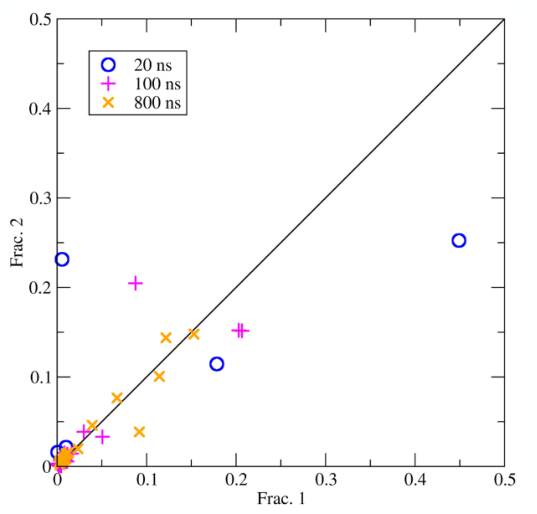
\includegraphics[scale = 0.4]{independent-simulations}
			\caption{Combined clustering}
			\label{fig:independent_simulation}
		\end{figure}

	\subsection{Equilibration and production}
	It can be seen in the case of slowly-equilibrating of figure \ref{fig:equilibration} a drift can be observed so there is no certainty of equilibration.

	\begin{figure}[H]
		\centering
		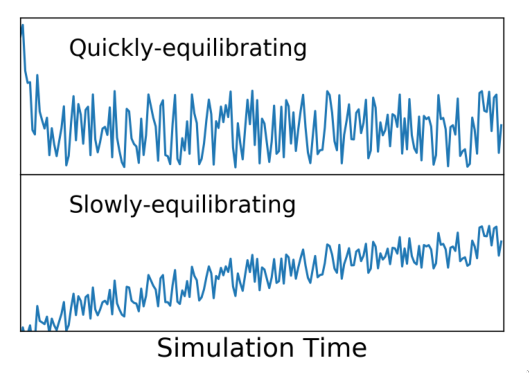
\includegraphics[scale = 0.5]{equilibration}
		\caption{Behaviour during equilibration}
		\label{fig:equilibration}
	\end{figure}

	Once we are confident that equilibration has been reached the trajectory has to be separated into the equilibration and production part.
	This can be seen in \ref{fig:equilibration-production}.
	Now equilibration is discarded and no longer considered in the analysis.
	In the analysis just the production will be considered.

	\begin{figure}[H]
		\centering
		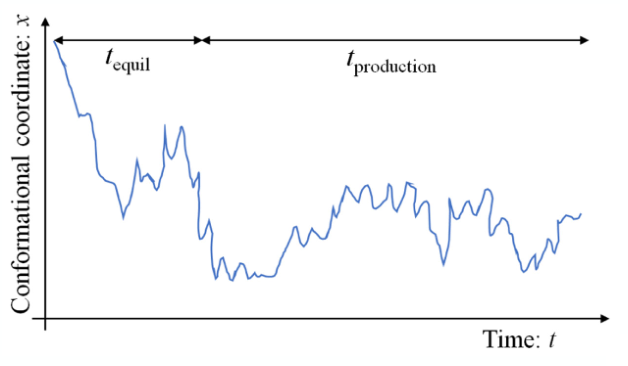
\includegraphics[scale = 0.5]{equilibration-production}
		\caption{Comparison of equilibration and production}
		\label{fig:equilibration-production}
	\end{figure}

	\subsection{Equilibration workflows}
	For the equilibration there are different type of workflow and the choice depends on the system in use.

		\subsubsection{First workflow}
		In this first workflow the simulated times are the physical time as in the NVE ensemble the Hamiltonian dynamics are considered because there is no thermostat.
		So this is a good workflow for observing dynamical properties.

		$$\overbrace{\underbrace{NVT}_{\substack{\text{short simulation to}\\\text{relax to temperature}\\\text{of interest}}}\rightarrow \underbrace{NVE}_{\text{short equilibration}}}^{\text{Suggested equilibration workflow}}\rightarrow \overbrace{NVE}^{\text{Production ensemble}}$$

		\subsubsection{Second workflow}
		In this second workflow the volume is kept fixed, the first simulation is used to adapted to the temperature and then the simulation is run.
		In this case the simulation is run at fixed density.
		This would be used for a liquid material.


		$$\overbrace{\underbrace{NVT}_{\substack{\text{short simulation to}\\\text{relax to temperature}\\\text{of interest}}}}^{\text{Suggested equilibration workflow}}\rightarrow \overbrace{\underbrace{NVT}_{\text{at known, fixed density}}}^{\text{Production ensemble}}$$


		\subsubsection{Third workflow}
		This third workflow is typical for proteins.
		So a combination of NPT and NVT to converge the volume and then the system is simulated without a barostat.

		$$\overbrace{\underbrace{NVT}_{\substack{\text{short simulation to}\\\text{relax to temperature}\\\text{of interest}}}\rightarrow \underbrace{NPT}_{\substack{\text{short simulation to}\\\text{relax to density of}\\\text{interest}}}\rightarrow\underbrace{NPT}_{\substack{\text{to compute average}\\\text{box size}}}\rightarrow \underbrace{NVT}_{\text{short equilibration}}}^{\text{Suggested equilibration workflow}}\rightarrow\overbrace{\underbrace{NVT}_{\substack{\text{for density defined by}\\\text{ pressure or unknown system}\\\text{density distribution,}\\\text{like a homogeneous system}}}}^{\text{Production ensemble}}$$

		\subsubsection{Forth workflow}
		This is a typical simulation for a membrane protein.

		$$\overbrace{\underbrace{NVT}_{\substack{\text{short simulation to}\\\text{relax to temperature}\\\text{of interest}}}\rightarrow \underbrace{NPT}_{\substack{\text{short simulation to}\\\text{relax to density of}\\\text{interest}}}}^{\text{Suggested equilibration workflow}}\rightarrow	\overbrace{NPT}^{\text{Production ensemble}}$$

\section{Autocorrelation}

	\subsection{Autocorrelation function}
	The autocorrelation function is useful to understand whether a system is equilibrated enough and how many independent conformations there are in the analysis.
	This is possible only when the correlation time is computed for an observable.
	So there is an autocorrelation function and time for each observable.
	Let $f(x)$ an observable, a function of the coordinates or the momenta.
	Then the autocorrelation function:

	$$C_f(t') = \frac{\bigl\langle(f(x)-\langle f\rangle)(f(t+t') - \langle f\rangle)\bigr\rangle}{\sigma^2_f}$$

	When $t'=0$ $C_f(t') = 1$.
	This function will decrease with $t'$.
	Using both the equilibration and production part of the simulation $C_f(t')$ will also depend on time time $t$.
	Using only the production run the dependence of $t$ is lost and the autocorrelation function can be computed.
	The function will go to $0$ with an exponential behaviour and fluctuate around that value.
	Performing this on a discretized time and the time ordered sequence of values $f_j = f(t=j\Delta t)$:

	$$C_f(t') = \frac{1}{\sigma^2_f}\frac{1}{N}\sum\limits_{j=1}^{N-\frac{t'}{\Delta t}}(f(j\Delta t)-\langle f\rangle)(f(j\Delta t + t')-\langle f\rangle)$$

	Computing the autocorrelation function starting after an increasing time if the system has equilibrated within the first time chosen the curves superimpose in the first part.

	\subsection{Autocorrelation time}
	The autocorrelation time is defined as:

	$$\tau_f = \int_0^{+\infty} dt' C_f(t')$$

	If the autocorrelation function is an exponential this is a good way to estimate the autocorrelation time.
	Looking at figure \ref{fig:autocorrelation-time}, although it seems that after $200ps$ the autocorrelation time is reached in this way the number of independent conformation is obtained.
	It could be that this number is not sufficient to sample the system properly.
	In that case the system is spending too much time in one conformation and not according to the Boltzmann distribution.
	The autocorrelation time will provide an idea on how many independent conformation there are in the syste,

	\begin{figure}[H]
		\centering
		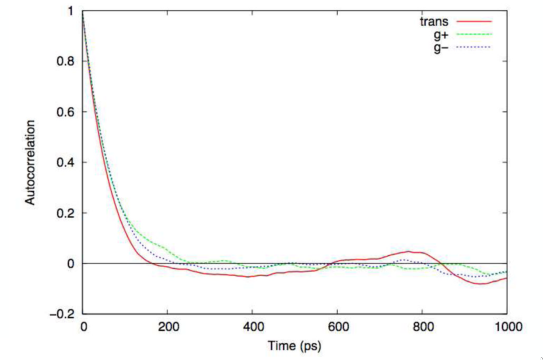
\includegraphics[scale = 0.6]{autocorrelation-time}
		\caption{Autocorrelation time}
		\label{fig:autocorrelation-time}
	\end{figure}

	The autocorrelation time $\tau_f$ is specific for each observable $f$ and allows to obtain the number of independent values of $f$ in the simulation:

	$$N_f^{ind}\simeq\frac{t_{sim}}{\tau_f}$$

	Where $t_{sim}$ is the total simulation time.
	Once the number of independent value is estimated the standard deviation of the mean can be computed using this number:

	$$SE(f) = \frac{\sigma_f}{\sqrt{N_f^{ind}}}\sim\sigma_f\sqrt{\frac{\tau_f}{t_{sim}}}$$

	A confidence interval at $95\%$ implies: $\pm 2 SE(f)$.

\section{Block averaging analysis}
The block averaging analysis is another way to compute the autocorrelation time.
In this method a trajectory with $N = M\cdot n$ snapshots is divided into $M$ segments of length $n$ with $n =1, 2, \dots$.
Compute $M$ averages, one in each block:

$$\langle f\rangle_i, \qquad i = =1, \dots, M$$

Compute the standard deviation $\sigma_n$ for each value of $n$.
Running estimate of the overall standard error:

$$BSE(f, n) = \frac{\sigma_n}{\sqrt{M}}$$

For small values of $n$ and high values of $M$, the $BSE$ under-estimates the statistical error.
The $BSE$ is constant once the blocks are essentially independent of one another, or when the block length is substantially greater than the correlation time.


\begin{multicols}{2}

	\begin{figure}[H]
		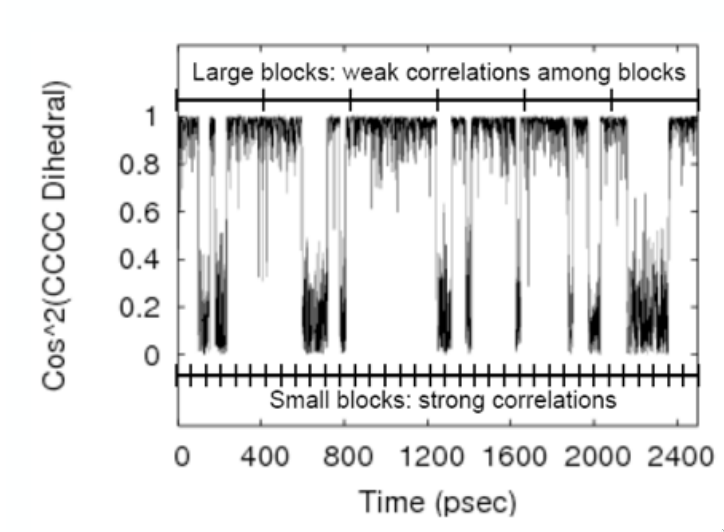
\includegraphics[width = 0.45\textwidth]{block-length}
		\caption{Varying block length}
		\label{fig:block-length}
	\end{figure}

	\columnbreak

	\begin{figure}[H]
		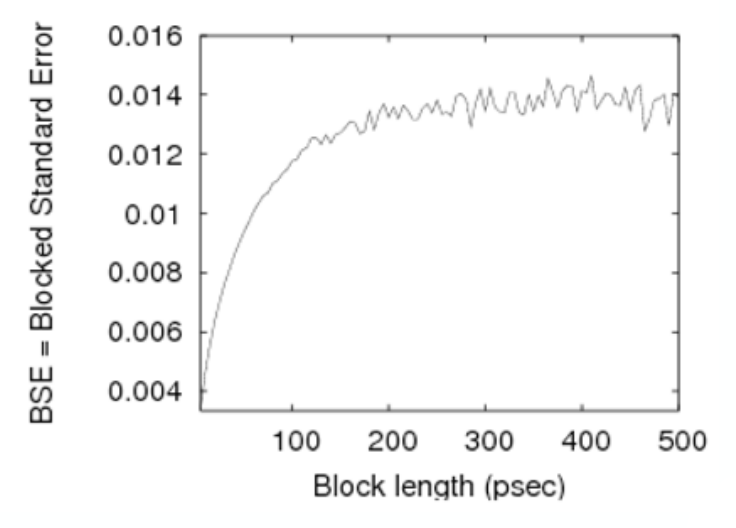
\includegraphics[width = 0.45\textwidth]{bse}
		\caption{BSE at varying block length}
		\label{fig:bse}
	\end{figure}

\end{multicols}

  % \graphicspath{{chapters/15/images/}}
\chapter{Protein motions}

\section{Elastic network models (ENM)}
In elastic network models ENM the structure of the protein is considered, with no attention to the kind of interactions.
The focus is on the topology: the protein is seen as a network of springs that connect beads.

\begin{figure}[H]
	\centering
	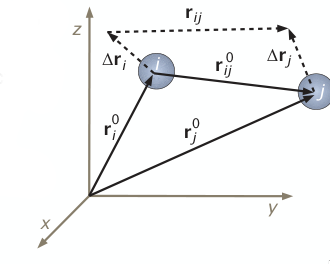
\includegraphics[scale = 0.5]{enm-theory}
	\caption{Elastic network models}
	\label{fig:enm-theory}
\end{figure}

Now considering the Gaussian network model, a kind of elastic network model.
Let $i$ and $j$ be two amino-acids as seen in \ref{fig:enm-theory}.
Usually the analysis is limited to centroids of residues: its $\alpha$-carbon atom.
A protein is represented by a configuration vector with the position of all its $\alpha$-carbon atoms: $\vec{r} = [\vec{r}_1, \vec{r}_2, \dots, \vec{r}_N]$.
It can be assumed that the structure obtained from the protein data bank is equilibrated.
Now computing the deviation of each $\alpha$-carbon atom from the equilibrium position (PDB structure):

$$\Delta\vec{r}_i = \vec{r}_i-\vec{r}_i^0$$

Instantaneous changes in the positions of all residues can be recorded in a vector with $3N$ components:

$$\Delta\vec{r} = [\Delta\vec{r}_1, \Delta\vec{r}_2, \dots, \Delta\vec{r}_N]$$


The equilibrium separation between two beads $i$ and $j$: $\vec{r}_{ij}^0 = \vec{r}_j^0-\vec{r}_i^0$.
The instantaneous separation between two beads $i$ and $j$: $\vec{r}_{ij} = \vec{r}_{ij}^0+\Delta\vec{r}_{ij}$, $\Delta\vec{r}_{ij} = \Delta\vec{r}_i-\Delta\vec{r}_i$.

	\subsection{Gaussian network model (GNM)}
	In Gaussian network model a potential energy is built up and it is assumed that each couple interact through an harmonic potential.
	So the potential energy for each couple:

	$$U_{ij} = \gamma_{ij}(\Delta\vec{r}_j-\Delta\vec{r}_i)\cdot(\Delta\vec{r}_j-\Delta\vec{r}_i) = \gamma_{ij}\Delta\vec{r}_{ij}^2$$

	Where the constant $\gamma$ depends on the couple of amino acid that are interacting.
	Now total elastic energy can be written as:

	$$U_{GNM} = \frac{1}{2}\sum\limits_i\sum\limits_j\gamma_{ij}\Delta\vec{r}^2_{ij} = \frac{\gamma}{2}\sum\limits_i\sum\limits_j\Delta\vec{r}_{ij}^2$$

	Another assumption, which is less problematic than the first one, does not affect the result.
	This assumption states that all amino acids that are interacting they interacting with the same constant $\gamma$ for all the couples there are.
	All the spring between the beads are the same.
	An interaction between two $\alpha$-carbon happens when they are closer than a cut-off radius usually set at $r_c = \si{\angstrom}$.
	Now Kirchhoff adjacency matrix $\Gamma$ is built, such that there is a $1$ (the sign is a convention) whenever there is an interaction or $0$ otherwise.
	This matrix will be symmetrical and the negative of the sum of rows or column and will be put on the diagonal.
	So in the diagonal there is the number of neighbours for each bead.

	\begin{figure}[H]
		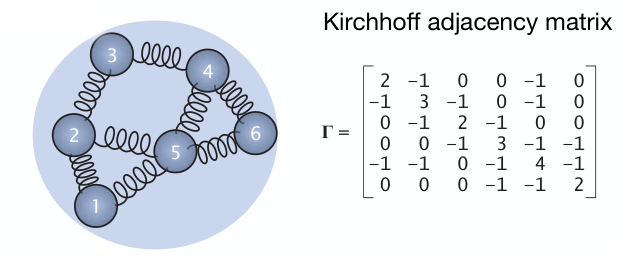
\includegraphics[width=\textwidth]{kirchoff-adjacency-matrix}
		\caption{Kirchhoff adjacency matrix}
		\label{fig:kirchhoff-adjacency}
	\end{figure}

	So the total elastic energy:

	$$U_{GNM} = \frac{\gamma}{2}\Delta\vec{r}(t)^T\Gamma\Delta\vec{r}(t)$$

		\subsubsection{Correlated motions}
		The average of displacement for each amino-acid and the correlated motion, so whether the displacement of an amino-acids correlates with the movement of another.
		To do so:

		$$\langle\Delta\vec{r}_i\cdot\Delta\vec{r}_j\rangle = \frac{1}{Q}\int\Delta\vec{r}_i\cdot\Delta\vec{r}_je^{-\frac{U}{kT}}d^N\Delta\vec{r}$$

		Since $U$ can be written as a matrix product the integral is a generalized Gaussian integral:

		$$\langle\Delta\vec{r}_i\cdot\Delta\vec{r}_j\rangle = \frac{3kT}{\gamma}[\Gamma^{-1}]_{ij}$$

		So that it can be exactly computed.
		Where $\Gamma^{-1}$ is a pseudoinverse matrix as the Kirchhoff matrix has zero determinant and cannot be inverted.
		To build the pseudoinverse matrix consider the eigenvalue decomposition: $\Gamma = U\Lambda U^T$:

		$$U = [\vec{u}_1, \dots, \vec{u}_{N_1}] = \begin{bmatrix} u_{1,1} & \cdots & u_{N-1,1}\\\vdots & \cdots & \vdots\\ u_{1, N} & \cdots & u_{N-1, N}\end{bmatrix}\qquad\Lambda = \begin{bmatrix} \lambda_1 & 0 & 0 & \cdots & 0\\ 0 & \lambda_2 & 0 &\cdots & 0\\0 & 0& \lambda_3 & \cdots & 0\\\vdots & \vdots & \vdots & \vdots &\vdots\\ 0 & 0 & 0 & \cdots & \lambda_{N-1}\end{bmatrix}$$

		Where $U$ is the matrix of eigenvectors and $\lambda_0$ is discarded.
		The pseudoinverse matrix is obtained by this matrix multiplication discarding $\lambda_0$ in $\Lambda$.

		\subsubsection{Gaussian network model and B-factors}
		The average fluctuation and the correlation of amino-acids.
		If $i=j$ the average fluctuation for each fluctuation, which can be obtained from the diagonal elements of the pseudoinverse matrix:

		$$\langle\Delta\vec{r}_i\cdot\Delta\vec{r}_i\rangle = \frac{3kT}{\gamma}[U\Lambda^{-1}U^{T}]_{ii} = \frac{3kT}{\gamma}\sum\limits_{k}[\lambda_k^{-1}\vec{u}_k\vec{u}_k^T]_{ii} = \sum\limits_{k}[\Delta r_i^2]_k$$

		The root-mean squared deviation can be represented as a sum of fluctuation for each of the modes or eigenvectors.
		Considering the Debye-Waller factors:

		$$B_i = \frac{8\pi^2}{3}\langle\Delta r_i^2\rangle$$

		Which are found in the PDB file and the factor $\gamma$ can be obtained by comparison of a result of the Gaussian network model so that the data look similar to the Debye-Waller factors.
		In figure \ref{fig:gnn-b-factors} the Debye-Waller are the continuous line while the dotted line is the average fluctuation computed from the Gaussian network model.
		Pay attention to proximity effects that arise from the crystal structure.

		\begin{figure}[H]
			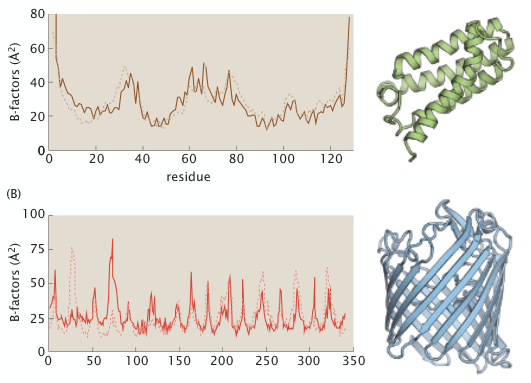
\includegraphics[width=\textwidth]{gnm-b-factors}
			\caption{GNM and B-factors}
			\label{fig:gnn-b-factors}
		\end{figure}

		\subsubsection{Biological relevance}
		Focussing on the slow of figure \ref{fig:biological-relevance} the contribution of each mode to the root mean squared deviation scales with the $-1$ power with respect to the eigenvalues: the smaller eigenvalue contribute more to the fluctuation and are the one more spread over the region of the protein.
		Looking at the fast mode with high eigenvalue are usually concentrated and characterized with spikes and are localized on amino-acids that corresponds to hydrophobic pocket of the protein and are fundamental for their structure.
		Inserting a mutation on one of the amino-acids could make the structure unstable.

		\begin{figure}[H]
			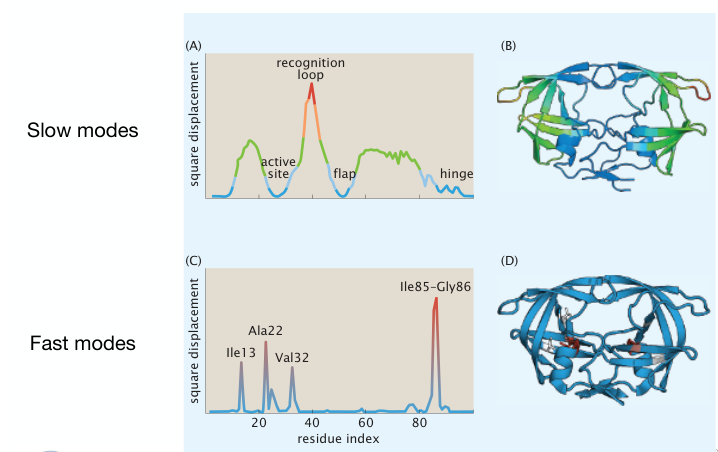
\includegraphics[width=\textwidth]{biological-relevance}
			\caption{Biological relevance}
			\label{fig:biological-relevance}
		\end{figure}

		\subsubsection{Normal mode analysis}
		Assuming that the approximation of the GNM is too crude and considering the fact that there are $3N-6$ degree of freedom.
		To be more rigorous the atomistic force field should be used and expand the potential function through a Taylor expansion around an equilibrium position:

		$$U = U_0 + \sum\limits_i\frac{\partial U}{\partial q_i}\biggr\rvert_{q^0}(q_i-q_i^0) + \frac{1}{2}\sum\limits_i\sum\limits_j\frac{\partial^2 U}{\partial q_i\partial q_j}\biggr\rvert_{q^0}(q_i-q_i^0)(q_j-q_j^0) + \cdots$$

		If $q^0$ represent the equilibrium the sum of the forces and in turn the first order term will be equal to $0$, so at equilibrium:

		$$U = \frac{1}{2}\Delta\vec{q}^TH\Delta\vec{q} = \frac{1}{2}\sum\limits_i\sum\limits_j H_{ij}(q_i-q_i^0)(q_j-q_j^0)$$

		Where $H$ is the Hessian matrix:

		$$H_{ij} = \frac{\partial^2 U}{\partial q_i\partial q_j}\biggr\rvert_{q^0}$$

		A matrix that can be computed analytically or numerically.
		This process is expensive because numerical derivatives have to be taken, but it is cheaper with respect to a molecular dynamics simulation.
		Now a covariance matrix can be computed:

		$$C = \langle\Delta\vec{q}\Delta\vec{q}^T\rangle = \frac{1}{Q}\int\Delta\vec{q}\Delta\vec{q}^Te^{-\frac{\Delta\vec{q}^TH\Delta\vec{q}}{2kT}}d^N\Delta\vec{q} = kTH^{-1}$$

		Where $H^{-1}$ is a pseudoinvers as the Hessian matrix will have $6$ $0$-eigenvalues because the degrees of freedom are $3N-6$ because overall translations and rotations are excluded.

	\subsection{Anisotropic network model (ANM)}
	In the anisotropic network model a normal mode analysis is performed, while assuming that each pair of interacting amino-acids have the same constant $\gamma$ and there is an harmonic potential between them:

	$$U_{ANM} = \frac{1}{2}\sum\limits_{ij}\gamma(r_{ij}-r_{ij}^0)^2\Rightarrow\frac{\partial^2 U}{\partial x_i\partial y)i} = -\gamma\frac{(x_i-x_i)(y_i-y_j)}{t_{ij}^2}$$

	So now the Hessian matrix can be computed easily:

	$$H_{ij} = \frac{\gamma}{r_{ij}^2}\begin{bmatrix}x_{ij}^2 & x_{ij}y_{ij} & x_{ij}z_{ij}\\x_{ij}y_{ij} & y_{ij}^2 & y_{ij}z_{ij}\\ x_{ij}z_{ij} & y_{ij}z_{ij} & z_{ij}^2\end{bmatrix}$$

	This matrix will be a $N\times N$ matrix with each amino acid and all the elements are $3\times 3$ matrices.
	Now the eigenvalue decomposition $H=U\Lambda U^T$ can be performed and the $0$-eigenvalue will be discarded.

	$$\Lambda = \begin{bmatrix}\lambda_1 & 0 & 0 & \cdots & 0\\ 0 & \lambda_2 & 0 & \cdots & 0\\ 0 & 0 & \lambda_3 & \cdots & 0\\\vdots & \vdots & \vdots & \vdots & \vdots\\ 0 & 0 & 0 & \cdots & \lambda_{3N-6}\end{bmatrix}$$

		\subsubsection{Correlated motions}
		Computing now the correlation between amino-acids and focussing on the specific motion of each mode represented by an eigenvector.

		$$\langle\Delta\vec{r}_i\cdot\Delta\vec{r}_j\rangle = \frac{3kT}{\gamma}[U\Lambda^{-1}U^T]_{ij} = \frac{3kT}{\gamma}\sum\limits_{k}\lambda_k^{-1}[\vec{u}_k\vec{u}_k^T]_[ij]$$

		The displacement of a protein can be computed from the modes.
		The direction of each mode is considered.
		This model does not treat all direction as the same.

		\begin{figure}[H]
			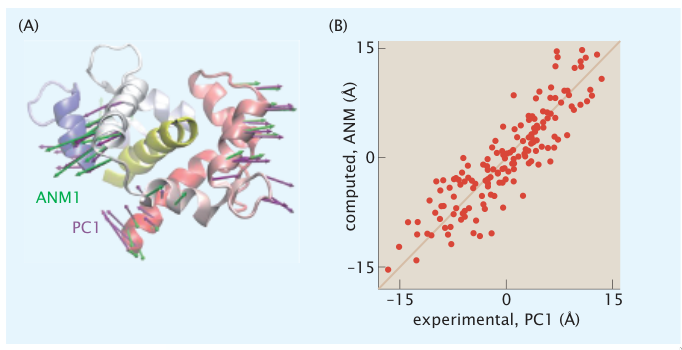
\includegraphics[width=\textwidth]{asm-correlated-motion}
			\caption{Correlated motions}
			\label{fig:as-correlated-motion}
		\end{figure}

		There are other instructive quantities that tells something more on the motion of the protein.
		For example the correlation cosine: projecting an eigenvector to the displacement between state $A$ and $B$ of the protein.
		The objective is to determine whether the transition was determined by the mode in consideration.
		The correlation cosine is computed as:

		$$I_k = \frac{\Delta\vec{q}_{AB}\cdot\vec{u}_k}{|\Delta\vec{q}_{AB}|}\qquad \Delta\vec{q}_{AB} = \vec{q}^B-\vec{q}^A$$

		The cumulative overlap is the number of mode that contribute to a motion:

		$$C_0 = \sqrt{\sum\limits_k I_k^2}$$

		Another quantity is the degree of collectivity, which will also be used in PCA.
		It is a factor that looks like a Shannon-entropy and it is defined as:

		$$\kappa_k = N^{-1}e^{-\sum\limits_{i=1}^N\alpha(\Delta r_i)^2\rvert_k\log(\alpha\Delta r_i)^2\rvert_k}$$

		Where $\alpha$ is normalized.

		$$\sum\limits_{i=1}^N\alpha(\Delta r_1)^2\rvert_k = 1$$

		When the degree of collectivity is close to $1$ there is a collective mode, so a mode that involves a large number of residues, while when it is close to $0$ the motion is localized on some portion of the protein.

\section{Essential dynamics}
Essential dynamics is based on principal component analysis: once a trajectory is obtained from a molecular dynamics simulation, the objective is to reduce the number of degrees of freedom to just those that are relevant to describe the motion of the system.
Not all of the degrees of freedom and a proper transformation of variable can be found so that the relevant of degrees of freedom are found.
They can be computed starting from the result of a molecular dynamics simulation.

\begin{enumerate}
	\item Obtain trajectories from molecular dynamics simulations, better if equilibrated.
		Equilibration is not mandatory as the new set of coordinates can be not equilibrated.
		There might be more than one trajectory that can be compared.
	\item Remove overall translations and rotations by aligning each frame to a reference structure.
		The reference frame can be the starting frame.
	\item Choose the set of atoms for the analysis like $\alpha$-carbons.
		In principle this analysis can be performed on all the atoms, but this is pointless.
		It is better to select on a subset of atoms, focussing on $\alpha$-carbons or on one sub-region of the protein.
	\item Obtain the covariance matrix:

		$$C_{ij} = \bar{(x_i(t) - \bar{x_i(t)})(x_j(t)-\bar{x_j(t)})}$$

		The covariance matrix is an average in time.
	\item If the fluctuations display some non-homogeneous behaviour, for example when there are loops that fluctuates a lot, it is better to employ the correlation matrix:

		$$R_{ij} = \frac{\bar{(x_i(t)-\bar{x_i(t)})}\bar{(x_j(t)-\bar{x_j(t)})}}{\sigma_{x_i}\sigma_{x_j}}$$

		Which is the covariance matrix normalized by the standard deviation.
	\item Diagonalize $C$ or $R$ employing eigenvalue decomposition EVD as in elastic network models.
	\item Examine the eigenvalue scree plot to determine the number of eigenvectors to include in the reduced vector space that describes the most relevant features.
		An example can be seen in figure \ref{fig:eigenvalue-scree-plot}.
		It can be seen how after a number of eigenvalues the other components have small eigenvalues.
		This behaviour is typical for a protein simulation, if the interaction describe a network.

	\begin{figure}[H]
	\centering
		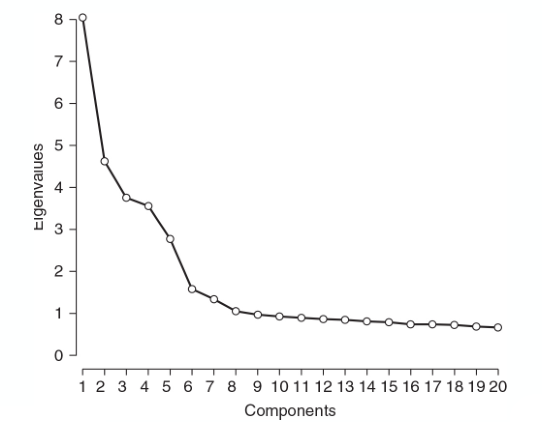
\includegraphics[scale = 0.5]{eigenvalue-scree-plot}
		\caption{Eigenvalue scree plot}
		\label{fig:eigenvalue-scree-plot}
	\end{figure}

\item Select the top set of eigenvectors to form the principal components (PCs) (usually between $2$ an $20$).
\item Examine the eigenvector collectivity for each mode defined as in the ANM: top modes tend to be more collective than lower modes, indicating that many residues are participating in collective motions.

	\begin{figure}[H]
	\centering
		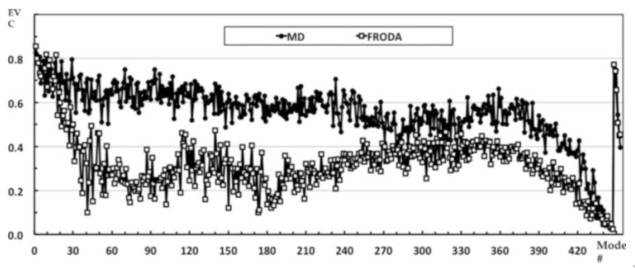
\includegraphics[scale = 0.4]{eigenvalue-collectivity}
		\caption{Eigenvalue collectivity}
		\label{fig:eigenvalue-collectivity}
	\end{figure}

\item Construct the weighted RMSD modes $\langle\Delta\vec{r}_i^2\rangle_k = \lambda_k[\vec{u}_k\vec{u}_k^T]_{ij}$.
	Visualize which residues contribute most to the fluctuation of each PCA mode.
	Comparing against the overall RMSF and looking where the most important contribution on the movement as in \ref{fig:weighted-rmsd}

	\begin{figure}[H]
	\centering
		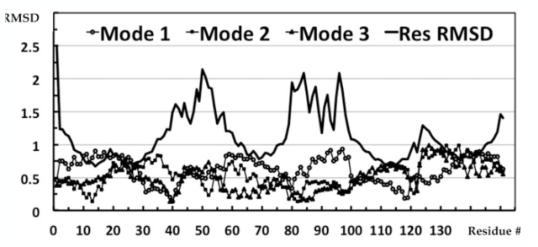
\includegraphics[scale = 0.4]{weighted-rmsd}
		\caption{Weighted RMSD modes}
		\label{fig:weighted-rmsd}
	\end{figure}

\item Construct the displacement vectors $\vec{d}_i(t) = \vec{r}_i(t)-\bar{\vec{r}_i}$ for each snapshot and construct the PCs projecting the displacement vectors onto the eigenvectors obtained:

	$$PC_k(t) = \sum\limits_{i=1}^N\vec{d}_i(t)\cdot\vec{u}_i^k\qquad\text{ with }k=1, \dots, 3N-6$$

	Each snapshot now is described by a single point with $3N-6$ numbers.
	Looking at these point in the multi-dimensional space and plotting them onto the first two principal component as in figure \ref{fig:scatter-plot-pcs-modes}.

	\begin{figure}[H]
	\centering
		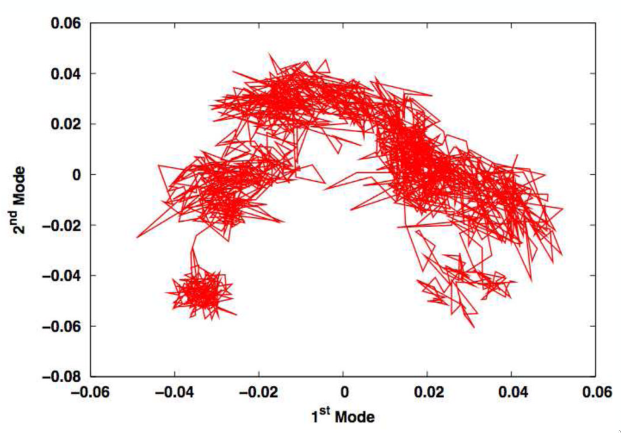
\includegraphics[scale = 0.4]{scatter-plot-pcs-modes}
		\caption{Scatter plot of first and second mode for PCs}
		\label{fig:scatter-plot-pcs-modes}
	\end{figure}

	The snapshots can be coloured according to time so to see the movement in the space as in figure \ref{fig:scatter-plot-pcs}

	\begin{figure}[H]
		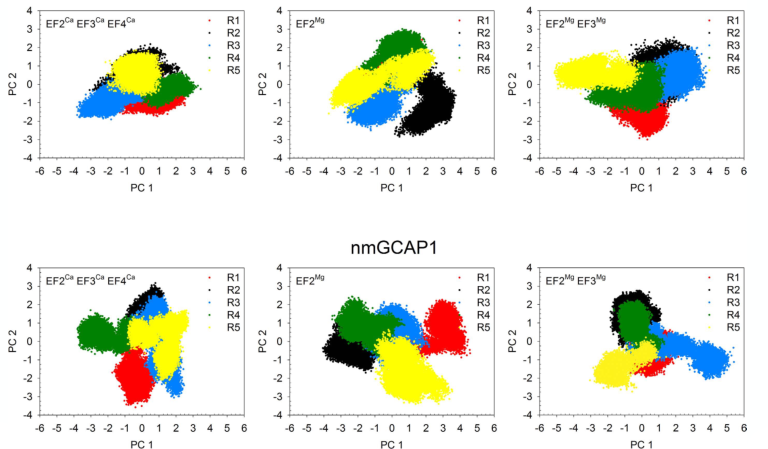
\includegraphics[width=\textwidth]{scatter-plot-pcs}
		\caption{Scatter plot of PCs, different replicas, the color indicates time of simulation.}
		\label{fig:scatter-plot-pcs}
	\end{figure}

\item Examine the cosine content for each mode $k$, defined as the superposition with the cosine obtained from a simple diffusion in a high dimensional harmonic potential:

	$$c_k = \frac{2}{T_{sim}}\biggl(\int_0^{T_{sim}}\cos\biggl(\pi\frac{k_BT}{\lambda_k}t\biggr)PC_k(t)dt\biggr)^2\biggl(\int_0^{T_{sim}}PC_k^2(t)dt\biggr)^{-1}$$

	The cosine content compares the principal component, which are a function of time, representing a time-series to the trajectory with the cosine that represents the diffusion of the system in a high-dimensional harmonic potential.
	If it is equal to $1$ one single basin is being explore, so the smaller the better, so that the system explores more basins and has equilibrated.
	An example can be seen in \ref{fig:cosine-content}.
	It can be seen how the cosine content decrees along the time of the simulation.
	The error bars can be obtained performing several simulation or dividing a simulation into pieces.
	This is another way to measure whether the system has equilibrated or not.

	\begin{figure}[H]
	\centering
		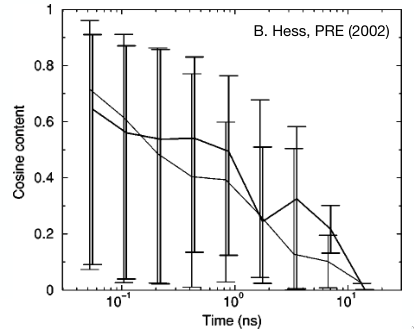
\includegraphics[scale = 0.6]{cosine-content}
		\caption{Cosine content for the modes}
		\label{fig:cosine-content}
	\end{figure}

\item Examine the similarity between trajectories or between portions of the same trajectory by examining the Covariance overlap:

	$$\Omega_{A, B} = 1 - \biggl[\frac{\sum\limits_{k=1}^{3N-6}(\lambda_k^A+\lambda_k^B)-2\sum\limits_{k=1}^{3N-6}\sum\limits_{j=1}^{3N-6}\sqrt{\lambda_k^A\lambda_j^B}(\vec{u}_k^A\cdot\vec{u}_j^B)^2}{\sum\limits_{k=1}^{3N-6}(\lambda_k^A+\lambda_k^B)}\biggr]^{\frac{1}{2}}$$

	$\Omega_{A, B} = 1$ if and only if the two covariance matrices are identical, while it is zero when the sampled subspaces are completely orthogonal.
\end{enumerate}

  % \graphicspath{{chapters/16/images/}}
\chapter{Clustering and protein structure networks}

\section{Introduction}
The aim of clustering is to find a way to group a set of data into clusters of similar properties.
This is done because:

\begin{multicols}{2}
	\begin{itemize}
		\item Labelling is expensive.
		\item To gain insight into the structure of data.
		\item Find prototypes in the data.
	\end{itemize}
\end{multicols}

In molecular simulations data usually refers to protein, DNA or RNA conformations.
So, given a set of data points, each described by a set of attributes, the clusters have to be found such that:

\begin{multicols}{2}
	\begin{itemize}
		\item Intra-cluster similarity is maximized: all the points in a cluster are as much similar as possible.
		\item Inter-cluster similarity is minimized: all the points between clusters are as much dissimilar between each other.
	\end{itemize}
\end{multicols}

	\subsection{Distance measures}
	To define similarity let $O_1$ and $O_2$ be two objects from the universe of possible objects.
	The distance or dissimilarly between $O_1$ and $O_2$ is a real number $D(O_1, O_2)$.
	A distance measure should have the following properties:

	\begin{itemize}
		\item Symmetry: $D(A,B) = D(B, A)$.
		\item Constancy of self-similarity: $D(A, A) = 0$.
		\item Positivity (separation): $(A, B) = 0\Leftrightarrow A=B$.
		\item Triangular inequality: $D(A, B) \le D(A, C) + D(B, C)$.
	\end{itemize}

	An example of this for molecular dynamics and two protein conformation is the root mean squared deviation, computing the all-to-all RMSD matrix.

	\subsection{Types of clustering}

	\begin{itemize}
		\item Hierarchical algorithms: create a hierarchical decomposition of the set of objects using some criterion.
		\item Partitional algorithms: construct various partitions and then evaluate them by some criterion,
	\end{itemize}

	\subsection{Distance measures}
	The distance between objects in a cluster or clusters can be computed in several ways:

	\begin{itemize}
		\item Single linkage or nearest neighbour: the distance between two clusters is determined by the distance of the two closest objects (nearest neighbours) in the different clusters.
		\item Complete linkage or furthest neighbour: the distance between two clusters is the greatest distance between two objects in the different clusters.
		\item Group average linkage: the distance between two clusters is computed as the average distance between all pairs of objects in the two different clusters.
	\end{itemize}

\section{Hierarchical clustering}

	\subsection{Dendrograms}
	In a dendrogram (\ref{fig:dendrogram}) the similarity between two objects is represented as the height of the lowest internal node they share.
	Each object is represented as a leaf.
	Dendrograms give a direct visual representation of the groups of data.

	\begin{figure}[H]
		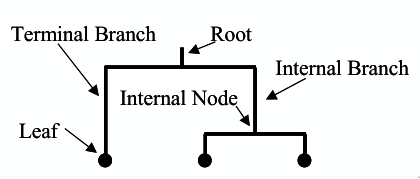
\includegraphics[width=\textwidth]{dendrogram}
		\caption{Dendrogram structure}
		\label{fig:dendrogram}
	\end{figure}

		\subsection{Interpretation}
		Hierarchical clustering sometimes show pattern that are meaningless or spurious.
		So the interpretation of the algorithm has to be performed.

		\subsection{Advantages of hierarchical clustering}

			\subsubsection{Correct number of clusters}
			One advantage of hierarchical clustering is that the correct number of cluster is obtained looking at the dendrogram.

				\begin{figure}[H]
					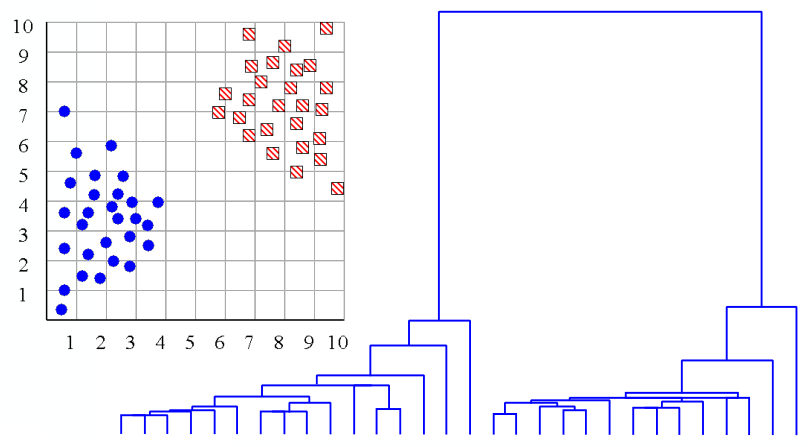
\includegraphics[width=\textwidth]{correct-number}
					\caption{Correct number of clusters}
					\label{fig:correct-number}
				\end{figure}

			\subsubsection{Outliers}
			Moreover when using hierarchical clustering the outliers are easily identified.

			\begin{figure}[H]
				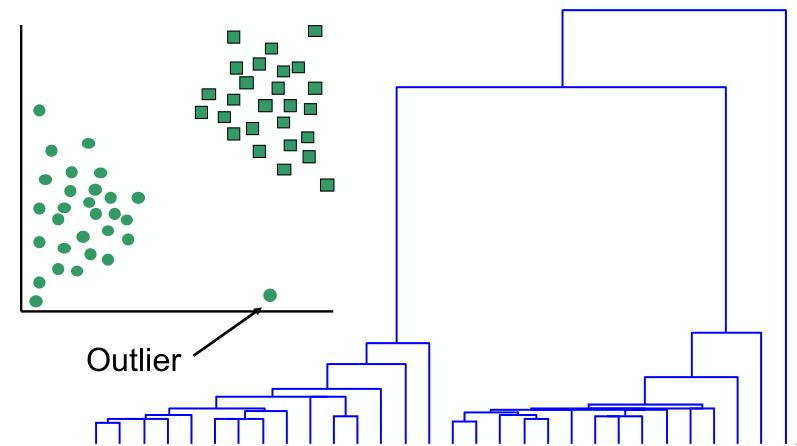
\includegraphics[width=\textwidth]{outliers}
				\caption{Outliers}
				\label{fig:dendrogram}
			\end{figure}

	\subsection{Hierarchical clustering approach}
	The number of dendrograms $D$ with $n$ leafs are:

	$$D = \frac{2n-3)!}{2^{n-2}(n-2)!}$$

	They can be built with two approaches:

	\begin{itemize}
		\item Bottom-up or agglomerative approach: each item is grouped alone into its own cluster and then the best pair to merge into a new cluster is found.
			This is repeated until all clusters are fused together.
		\item Top-down or divisive approach: all the data is grouped into a single cluster, then the best division into two cluster is chosen and this is repeated recursively on both sides.
	\end{itemize}

	\subsection{Summary of hierarchical methods}

	\begin{itemize}
		\item No need to specify the number of clusters in advance.
		\item The hierarchical nature maps nicely onto human intuition for some domains.
		\item They do not scale well: $O(n^2)$.
		\item The interpretation of the results is very subjective.
	\end{itemize}

\section{Partitional clustering}
In partitional clustering each item is placed in exactly one of $K$ non-overlapping clusters.
The number of cluster is provided as input.

	\subsection{K-means}

	\begin{enumerate}
		\item Choose the value $k$.
		\item Initialize the $k$ cluster centres randomly.
		\item Decide the class memberships of the $N$ objects by assigning them to the nearest cluster centre.
		\item Re-estimate the $k$-cluster centres by assuming the memberships found are correct.
		\item If non of the $N$ objects changed memberships in the last iteration exit, otherwise go back to step $3$.
	\end{enumerate}

		\subsubsection{Conclusion}

		\begin{itemize}
			\item Relatively efficient: $O(tkn)$ where $n$ is the number of objects, $k$ is the number of clusters and $t$ the number of iterations.
			\item It often terminates at a local optimum.
			\item It is applicable only when a mean can be defined.
			\item The number of cluster has to be specified in advance.
			\item It is unable to handle noisy data or outliers.
			\item It is not suitable to discover clusters with non-convex shapes.
		\end{itemize}

	\subsection{Sum of squared errors}
	The sum of squared error will be the objective function that determines how well the data is divided into clusters.

	$$SE_{K_i} = \sum\limits_{j=1}^m[D(C_{ij}, C_{K_i})]^2$$

	$$SE_K = \sum\limits_{i=1}^jSE_{K_i}$$

	\subsection{Choosing K}
	The optimal $k$ is the one such that the $\min SE$ is found.
	It can be chosen running the algorithm with iteratively increasing value of $k$ and looking at the Knee or elbow plot of $k$ in relation with $SE$ as in \ref{fig:elbow}.

	\begin{figure}[H]
		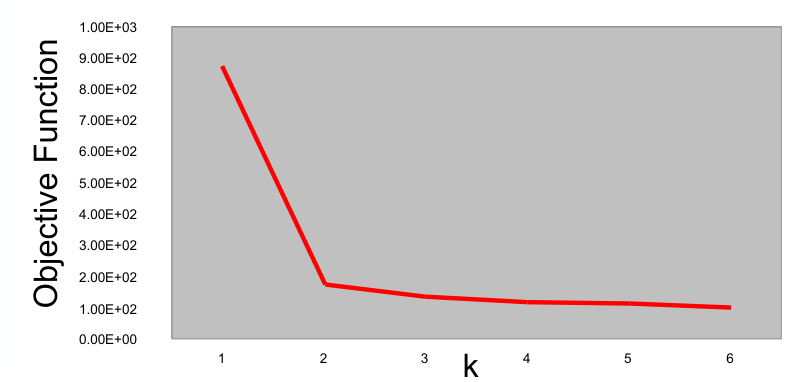
\includegraphics[width=\textwidth]{elbow}
		\caption{Knee or elbow plot}
		\label{fig:elbow}
	\end{figure}

\section{Protein structure networks}
Protein structure networks represents proteins as networks built after the molecular dynamics simulation is performed.

\begin{figure}[H]
	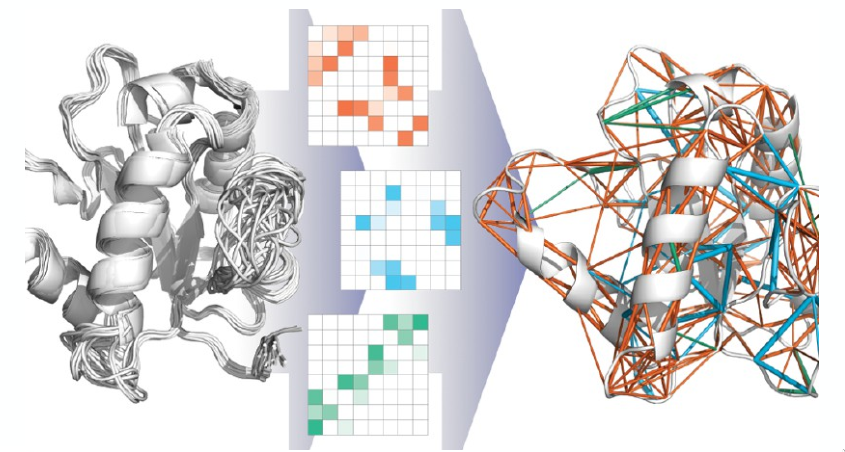
\includegraphics[width=\textwidth]{psn}
	\caption{Protein structure network}
	\label{fig:psn}
\end{figure}

	\subsection{PyInteraph}
	PyInteraph is an algorithm to analyse the trajectories.
	The protein is represented as a graph where the nodes are the side chains of protein residues and the edges can be defined in term of:

	\begin{multicols}{2}
		\begin{itemize}
			\item Distance.
			\item Atomic contacts.
			\item Van der Waals interactions.
			\item Interaction energy.
		\end{itemize}
	\end{multicols}

	Then a graph analysis approach to the intramolecular interaction network IIN is performed.

	\subsection{Classes of interactions}
	This interactions are non-bonded interactions that are not present in the force-field.

		\subsubsection{Hydrophobic contacts}
		In the hydrophobic contacts the centre of mass of the two side chains are distant less than $5\si{\angstrom}$.
		The centres of mass is specified by the force field for different masses, so they will be force-field specific.
		It has default residues, the typically hydrophobic residues that are checked by pyInteraph.

		\begin{multicols}{4}
			\begin{itemize}
				\item Ala.
				\item Ile.
				\item Val.
				\item Phe.
				\item Met.
				\item Trp.
				\item Pro.
			\end{itemize}
		\end{multicols}

		\subsubsection{Salt bridges}
		Salt bridges corresponds to the interaction of groups with opposite charge.
		They are formed between atom pairs belonging to two charged groups of two different residues with distance less than $4.5\si{\angstrom}$.

		\subsubsection{Hydrogen bonds}
		Hydrogen bond happen when the distance between the acceptor and the hydrogen atom is less than $3.5\si{\angstrom}$ and the donor-hydrogen-acceptor angle is greater than $120^\circ$.

	\subsection{Persistence}
	Persitence is the fraction of the number of structures in the ensemble in which the interaction was observed: the interactions are computed for each frame.
	For hydrogen-bond one or more interactions may exist between two residues.
	PyInteraph will generate interaction matrix for each type of interaction.
	Then for each interaction the edge weight is given, corresponding to the persistence value.
	Then these three interaction network are filtered according to a measure providing a persistence threshold.
	When the value of the persistence is higher than the threshold a contact is assumed true.
	After that the macro-intramolecular-interaction network that collects informations about all the different of interactions.

	\subsection{Persistence threshold}
	To choose the persistence threshold the connected components of the protein structure network have to be found.
	A connected component is a subgraph in which a path exists between any two vertices, but no path exist to any other vertices of the main graph: there are no edges connecting two connected components.
	After having obtained them for each value of the persistence, so that a connection is defined whenever the persistence is higher than the value.
	It can be seen how decreasing the threshold the size of the connected components increase.
	A typical graph of persistence over component size a kink can be found and that will be the persistence threshold.

	\subsection{Graph analysis}
	Some analysis provided by pyInteraph are:

	\begin{itemize}
		\item Computing the highly connected residues or hubs: residues with with more than $3$ or $4$ edges.
			A list of hubs and their respective connectivity degree (how many residue are connected to them) is computed.
			Hubs indicates that their residues will play a key role in the structure or function of the protein.
		\item Connected components.
			The groups and part of the protein are connected and can be assumed to behave as rigid object in the protein.
			These can find domains that behave mechanical in the same way in the protein.
		\item Shortest path between two specified residues.
			This is useful because many proteins have allosteric communication pathways and they could be explored by this analysis, finding the amino acids that transport the mechanical signal from one side of the protein to another.
	\end{itemize}

	\subsection{Examples}

		\subsubsection{p53 DNA binding domain}
		Hydrophobic interactions play a crucial role in the stabilization of the protein core and in the maintenance of the 3D structure and stability.
		In general hydrophobic interaction play a crucial role in the folding, structure and function of the protein.

		\begin{figure}[H]
			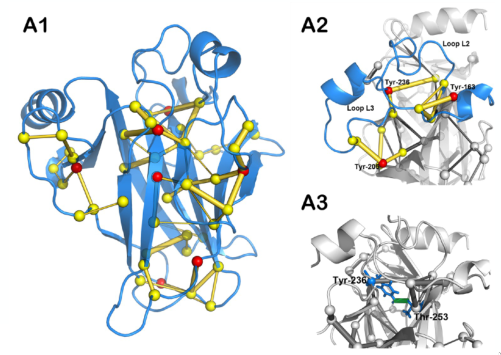
\includegraphics[width=\textwidth]{p53}
			\caption{p53}
			\label{fig:p53}
		\end{figure}

		\subsubsection{Vibrio proteinase (VAP)}
		Salt bridges or hydrogen bonds are highly flexible and cooperatively organized in networks across the protein structure or for temperature adapted organisms.

		\begin{figure}[H]
			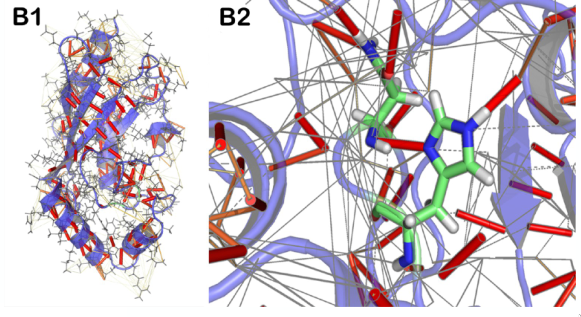
\includegraphics[width=\textwidth]{vap}
			\caption{VAP}
			\label{fig:vap}
		\end{figure}

  % \graphicspath{{chapters/17/images/}}
\chapter{Monte Carlo methods}

\section{Introduction}
Monte Carlo methods are based on games of chance.
The basic idea is to evaluate the value of integrals, for example:

$$I = \int_0^1dx\int_0^{\sqrt{1-x^2}}dy = \frac{\pi}{4}$$

This is done when analytical methods cannot be applied.

	\subsection{Central limit theorem}
	This method is important in statistical mechanics as the aim is to evaluate integrals that define the average value of a quantity.
	Let $f$ be a distribution function such that:

	$$f(x)\ge 0\qquad \int f(x)dx = 1$$

	And $\phi$ an arbitrary function.
	And the integral that has to be evaluated to obtain the average value.

	$$I = \int dx\phi(x)f(x)\equiv\langle\phi\rangle_f$$

	Let $x_1, \dots, x_M$ n-dimensional vectors sampled from $f(x)$.
	Then by the central limit theorem:

	$$\tilde{I}_M = \frac{1}{M}\sum\limits_{i=1}^M\phi(x_i)\qquad \lim\limits_{M\rightarrow\infty}\tilde{I}_M = I$$

	Now the average is a good estimator for the integral with some error considering the fluctuation of the function $\phi$ sampled by $f$:

	$$\int dx\phi(x)f(x) = \frac{1}{M}\sum\limits_{i=1}^M\phi(x_i)\pm\frac{1}{\sqrt{M}}\bigl[\langle\phi^2\rangle_f-\langle\phi\rangle_f^2\bigr]^{\frac{1}{2}}$$

	In this way beside a good estimate of the integral also the error can be evaluated.
	So increasing the number of points decrease the error.

	\subsection{Sampling distributions}
	Random number generators are fundamental during Monte Carlo simulations.
	Consider a one dimensional distribution function:

	$$\int_a^bf(x)dx = 1\qquad f(x)\ge 0$$

	The cumulative probability is defined as:

	$$P(X) = \int_a^X f(x)dx\qquad X\in[a,b]$$

	$P(X)$ is the probability that any chosen $x$ from the distribution $f(x)$ lies in $[a, X]$.
	$P(X)$ is a monotonically increasing function of $X$, moreover:

	$$f(X) = \frac{dP}{dX}$$

	Performing a variable transformation $x\rightarrow y$ with $y = g(x)$ a non decreasing function of $x$:

	$$X\ge x \Rightarrow g(X) \ge g(x)$$

	Defining $\tilde{P}(Y=g(X))$ is the probability that $g(X)=Y\ge y\ge g(x)$, the probability that $X\ge x$, then:

	$$\tilde{P}(Y) = P(X)$$

	This allows to obtain random number distributed according to any distribution starting from any other.
	As an example:

	$$w(r) = \begin{cases}1 &0\le r\le 1\\0 &otherwise\end{cases}\qquad W(\xi) = \int_0^\xi w(r)ds = \begin{cases}0 & \xi<0\\\xi & 0\le\xi\le1\\1 &otherwise\end{cases}$$

	$W(\xi) = \xi$ is the probability that a value of $r$ that has been chosen randomly lies in $[0, \xi]$.
	Now the function $g$ has to be found such that $r = g(x)$ with $g(x)$ a non decreasing function: solve $P(X) = \xi$.

		\subsubsection{An example}
		Assume that random number has to be obtained using the function:

		$$f(x) = ce^{-cx}\qquad x\in[0, +\infty[$$

		Now computing the cumulative distribution function that corresponds to that distribution function and then assuming that $P(X) = \tilde{P}(Y)$, the cumulative distribution function for the uniform random number that was equal to $\xi$.
		In this way the relation between $X$ and $\xi$ is found.

		$$P(X) = \int_0^Xce^{-cx}dx = 1- e^{-cX} = \xi\Rightarrow X = -\frac{1}{C}\ln(1-\xi)$$

		Now any number obtained from the uniform distribution function is the value of $\xi$, which if it is plugged into the previous equation the number distributed according to the desired distribution is obtained.
		The same procedure can be generalized to more than one random variable easily when $f(x)$ is separable into a product of $n$ single-variable distributions.
		This is the procedure that most of the integrator employs to generate velocities and initial conditions to the momenta.

	\subsection{Importance sampling}
	Going back to the problem of the integral.
	Let $I$ be the integral of an observable $\phi$.

	$$I = \int dx\phi(x)f(x) = \int dx\biggl[\frac{\phi(x)f(x)}{h(x)}\biggr]h(x) = \int dx\psi(x)h(x)$$

	Let $h$ be another distribution function defining $\psi(x) = \frac{\phi(x)}{h(x)}$.
	Applying the central limit theorem:

	$$I = \int dx\psi(x)h(x) = \frac{1}{M}\sum\limits_{i=1}^M\psi(x_i)\pm\frac{1}{\sqrt{M}}[\langle\psi^2\rangle_h-\langle\psi\rangle_h^2]^{\frac{1}{2}}$$

	This is done because $h(x)$ might be easier to sample or it might behave better than $f(x)$.
	In the canonical ensemble for example it is better to compute first the Boltzmann-Weight of the conformation before sampling the conformation from the distribution function.
	Another distribution function instead of the original, so the optimal choice for this probability distribution function $h(x)$:

	$$\sigma^2[h] = \int dx\psi^2(x)h(x) - \biggl[\int dx\psi(x)h(x)\biggr]^2 = \int dx\frac{\phi^2(x)f^2(x)}{h(x)}-\biggl[\int dx\phi(x)f(x)\biggr]^2$$

	Minimize the functional $\sigma^2[h]$ with the constraint $\int dx h(x) = 1$ driven by the normalization of $h(x)$.
	To do so the methods of	Lagrange multiplier is used introducing an extra variable $\lambda$ and introducing the functional: $F[h] = \sigma^2[h]-\lambda\int dxh(x)$.
	Taking the functional derivative: $\frac{\delta F[h]}{\delta h(x)} = 0$ with $\delta F[h] = F[h+\delta h]-F[h]$ will allow to find an equation for $\lambda$ that will be made explicit using the normalization condition.
	The equality equal to $0$ to minimize $\sigma^2[h]$.
	Now using the Taylor expansion of the first factor on $\delta h$:

	\begin{align*}
		\delta F[h] &= \int dx\biggl[\frac{\phi^2(x)f^2(x)}{h(x) + \delta h(x)} - \frac{\phi^2(x)f^2(x)}{h(x)}\biggr]-\lambda\delta h(x)=\\
								&=-\frac{\phi^2(x)f^2(x)}{h^2(x)}\delta h(x)-\lambda\delta h(x)
	\end{align*}

	Now taking the derivative equal to $0$ an equation to obtain $h$ is found:

	$$\frac{\delta F[h]}{\delta h(x)} = 0\Rightarrow\frac{\phi^2(x)f^2(x)}{h^2(x)}+\lambda = 0\Rightarrow h(x) = \frac{1}{\sqrt{-\lambda}}\phi(x)f(x)$$

	Looking at the normalization condition:

	$$\int dxh(x) = 1\Rightarrow\sqrt{-\lambda} = \int dx\phi(x)f(x) = I$$

	So the optimal choice is $h(x) = \frac{\phi(x)f(x)}{I}\Rightarrow \sigma^2[h] =0$.
	Where $h$ is the function used in importance sampling.
	$I$ is needed, but it is the objective of this computation.
	This means that the true function $h$ cannot be obtained, but there are some tricks to generate a number of points distributed to the function $h$.
	This is called importance sampling and to sample the phase space according to the optimal choice of the distribution function the Metropolis algorithms will be used.
	In this way sampling is efficient and the estimate is a good one.
	A system will be simulated and points distributed according to $h$ will be extracted.

		\subsubsection{An example}
		Computing the integral:

		$$\int_0^1 dxe^{-x}$$

		It can be seen how the function to be integrate is the solid line ($\phi(x)$) in the left panel of figure \ref{fig:importance-sampling-example}.
		Two importance functions can be found: $1-x$ for the dotted line and $1-0.64x$ for the dashed one.
		Looking at the two functions using importance sampling convergence will be faster.
		Looking at the middle panel the result of sampling from $0$ and $1$ uniformly looking at the estimator of the integral.
		There are huge fluctuation.
		Using instead one of the two functions the convergence will be improved as in the right panel the fluctuation are much smaller.

		\begin{figure}[h]
			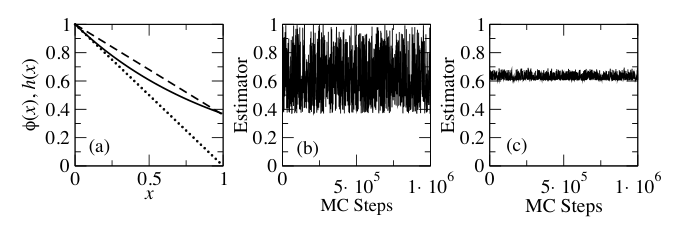
\includegraphics[width=\textwidth]{importance-sampling}
			\caption{The integrand and two possible importance functions}
			\label{fig:importance-sampling-example}
		\end{figure}

	\subsection{Molecular dynamics and Monte Carlo methods}
	In molecular dynamics:

	\begin{multicols}{2}
		\begin{itemize}
			\item All particles move at once, but the $\Delta t$ is usually quite small.
			\item Information on dynamics are available.
			\item Parallel architectures: molecular dynamics is more parallelizable and it is naturally implemented on parallel computers.
		\end{itemize}
	\end{multicols}

	In Monte Carlo:

	\begin{multicols}{2}
		\begin{itemize}
			\item There is no limit on the range of moves: the only limit is the Boltzmann weights, but also unphysical moves can be considered.
				The dynamics of the movement is not important.
			\item Natural thermostats and barostats: they are easily implemented in a Monte Carlo simulation.
			\item Flexibility: it can be applied to any possible system, playing with the moves makes it extremely flexible.
			\item Egodicity can be achieved thinking about a strange move that moves in the phase space.
		\end{itemize}
	\end{multicols}

\section{Markov chains}
A Markov chain is a rule to obtain the point at the next iteration starting from a point.
The state of the system depends only on the previous instant of time.
The vectors $x_1, x_2, \dots, x_M$ can be generated sequentially in a Markov chain: a rule to generate $x_{i+1}$ given $x_i$ is given.
This points will be sampled according to the same distribution from which we want to sample:

$$\tilde{I}_M = \frac{1}{M}\sum\limits_{i=1}^M\phi(x_i)$$

This rule is defined as $R(x|y)$,  the probability to obtain $x$ given $y$.
If there are two micro states it is the probability to move to a microstate $x$ from a microstate $y$.

	\subsection{Detailed balance condition}
	To define a rule a detailed balance condition is imposed

	$$R(x|y)f(y) = R(y|x)f(x)$$

	This means that the probability to go from $y$ to $x$ times the probability of being in $y$  is equal to the inverse movement.
	Some features of the detailed balance condition are:

	\begin{itemize}
		\item It represents microscopic reversibility.
		\item It is an unbiased sampling of phase space.
		\item It is sufficient but not strictly necessary condition to ensure proper sampling of phase space.
			Unbiased sampling can be obtained without the detailed balance condition.
	\end{itemize}

	\subsection{Rejection methods}
	Using the detailed balance condition a rejection method is built.
	Let $T(x|y)$ a rule to generate a trial move or proposed move from $y$ to $x$.
	This is the probability to go from $y$ to $x$ by the way the proposed move are constructed.
	This quantity is normalized:

	$$\int dxT(x|y) = 1$$

	So the probability to go from state $y$ to anywhere is $1$.
	Let $A(x|y)$ be the probability to accept the move from $y$ to $x$.
	Now the probability to go from $y$ to $x$ is the product of the probability of generating the move and the probability of accepting that move:

	$$R(x|y) = A(x|y)T(x|y)$$

	By applying the detailed balance condition:

	$$A(x|y)T(x|y)f(y) = A(y|x)T(y|x)f(x)$$

	By looking at this equation it can be seen how the acceptance probabilities are related.
	In this way the integral is cancel because it is at the denominator for $f$.
	If the algorithm is symmetrical the probability of the inverses moves is equal.
	The acceptance probability are related to each other and are not independent.
	Writing down this relation:

	$$A(x|y) = \frac{T(y|x)f(x)}{T(x|y)f(y)}A(y|x) = r(x|y)A(y|x)$$

	Where $\frac{T(y|x)f(x)}{T(x|y)f(x)} = r(x|y)$.
	If $A(x|y) = 1$ the move $y\rightarrow x$ is favoured $\Rightarrow A(y|x)< 1 \Rightarrow r(x|y)>1$.
	If $A(x|y) < 1$, $y\rightarrow x$ is not entirely favoured $\Rightarrow A(y|x) = 1\Rightarrow r(x|y) < 1$.
	Writing down this $A$ can be defined as:

	$$A(x|y) = \min[1, r(x|y)]$$

	So the acceptance probability of the move from $y$ to $x$ is the minimum between $1$ and $r(x|y)$.

	\subsection{Metropolis algorithm}
	In order to build the acceptance rate the trial distribution $T(x_{k+1}|x_k)$ has to be written to be able to propose a move $x_k\rightarrow x_{k+1}$ and being able to compute:

	$$r(x_{k+1}|x_k) = \frac{T(x_k|x_{k+1})f(x_{k+1})}{T(x_{k+1}|x_k)f(x_k)}$$

	If $r(x_{k+1}|x_k)>1$ accept the move, otherwise accept the move with probability given by $r(x_{k+1}|x_k)$: extract a random number $\xi\in[0,1]$.
	If $\xi< r(x_{k+1}|x_k)$ accept the move.
	Rejections do count: when a move is rejected that particular conformation will be counted twice because the importance sampling samples the system with a distribution function that is required by it, which means that points that are more representative for the representation functions will be explored more: if a move if rejected that point counts more in the average.

		\subsubsection{Proof}
		Associated probability for each point $x_1, \dots, x_n$: $\pi_1(x), \dots, \pi_n(x)$.
		With a huge number of moves the probability is equal to the desired distribution.

		$$\lim\limits_{n\rightarrow\infty}\pi_n(x) = f(x)$$

		Proof by recursive relation: $\pi_{n+1}(x)$ receives contributions from accepted moves starting at $y$ and ending in $x$ and from attempted moves to $y$ that are rejected:

		$$\pi_{n+1}(x) = \int A(x|y)T(x|y)\pi_n(y)dy + \pi_n(x)\int[1-A(y|x)]T(y|x)dy$$

		If $\pi_n(x) = f(x)$:

		$$\pi_{n+1} = \int A(x|y)T(x|y)f(y)dy + f(x)\int[1-A(y|x)]T(y|x)dy$$

		Considering the detailed balance condition: $A(x|y)T(x|y)f(y) = A(y|x)T(y|x)f(x)$ two terms cancel each other out:

		$$\pi_{n+1}(x) = f(x)\int T(y|x)dy = f(x)$$

		So if the system arrives at the distribution function $f$ it will stay there.

		\subsubsection{Summary}
		Everything sums up to evaluate the ratio of the final over probabilities of generating the moves to the initial and final states.

		$$r(x|y) = \frac{T(y|x)f(x)}{T(x|y)f(y)}$$

		The acceptance probability is computed according to:

		$$A(x|y) = \min[1, r(x|y)]$$

		For a uniform choice of $T(x|y)$, so the same probability from $x$ to $y$ and from $y$ to $x$:

		$$r(x|y) = \frac{f(x)}{f(y)}\Rightarrow A(x|y) = \min\biggl[1, \frac{f(x)}{f(y)}\biggr]$$

		Considering the Boltzmann distribution in this ratio the partition function would be cancelled.

	\subsection{Canonical distribution}
	In the canonical distribution the partition function, where the integrand is the Boltzmann weight:

	$$Q(N, V, T) = \frac{1}{N!\lambda^{3N}}\int d\vec{r}_1\cdots d\vec{r}_Ne^{-\beta U(\vec{r}_1, \dots, \vec{r}_N)}$$

	So the acceptance probability for a move from $r$ to $r'$ will be:

	$$A(r'|r) = \min\bigl[1, e^{-\beta(U(r')-U(r))}\bigr]$$

	$\Delta U < 0$ accept the move, so when decreasing the energy the move is accepted.
	$\Delta U > 0$ accept the move with probability $e^{-\beta\Delta U}$ if the energy has increased.
	In this way points that are distributed according to Boltzmann distribution can be simulated.
	Considering the acceptance, the Monte Carlo method will be efficient for an acceptance rate neither too high (not exploring enough) nor to low (never moving).
	The acceptance probability depends on the energy difference.
	Changing the coordinates of all the particles randomly it is highly probable to generate a huge energy difference (energy is an extensive quantity), causing the acceptance rate to be small.
	Because of this it is better to move the particles one by one.
	The particle to be updated should be chosen randomly because, when doing it sequentially the reverse move has not the same probability so the probability will not be symmetrical.
	A Monte Carlo pass is equivalent to $N$ trial moves: particles must be chosen randomly.
	On average each particle has seen at least one attempt to be moved.
	Considering a possible trial move:

	$$\begin{cases}x'_i = x_i+\frac{1}{\sqrt{3}}(\xi_x-0.5)\Delta\\y'_i = y_i+\frac{1}{\sqrt{3}}(\xi_y-0.5)\Delta\\z'_i = z_i+\frac{1}{\sqrt{3}}(\xi_z-0.5)\Delta\end{cases}$$

	Where $\xi$ is the random number, and the $0.5$ is needed to generate forward and backward moves, centring it around zero so to have the same probability to generate the backward move (when it is less than $0$).
	In one Monte Carlo pass each particle on average has seen one attempt.
	It is not necessary to recompute all the energy $U(r')$ in full at each move, because changing only the coordinates of one particle and taking its list of neighbours, the energy for that particle and list of neighbours are updated.
	$\Delta$ is the magnitude of the movement.
	If it is too big the probability to accept the move will be small.
	If it is too small the phase space is not being explored too well.
	As a rule of thumb after trying of simulation and keeping track of the acceptance rate, a good value should have an acceptance rate between $30$ and $50\%$.

\section{Simulating ensembles}

	\subsection{Isothermal-isobaric ensemble}
	Considering the partition function for the ensemble:

	$$\Delta(N, P, T) = \frac{1}{V_0} \int dVe^{-\beta PV}Q(N, V, T) = \frac{1}{V_0}\frac{1}{N!\lambda^{3N}}\int_0^{\infty}dVe^{-\beta PV}\int_Vd\vec{r}_1\cdots d\vec{r}_Ne^{-\beta U(\vec{r}_1, \dots, \vec{r}_N)}$$

	The scheme is the same as in the canonical ensemble with another trial move on the volume volume: $V' = V + (\xi_V-0.5)\delta$.
	The percentage of volume moves has to be chosen.
	Volume changes imply scaling of particle coordinates: $r'_i = \biggl(\frac{V'}{V}\biggr)^{\frac{1}{3}}r_i$.
	Making the dependance on volume explicit:

	$$\Delta(N, P, T) = \frac{1}{V_0}\frac{1}{N!\lambda^{3N}}\int_0^{\infty}dVV^Ne^{-\beta PV}\int_Vd\vec{s}_1\cdots d\vec{s}_Ne^{-\beta U(V^{\frac{1}{3}}\vec{s}_1,\dots, V^{\frac{1}{3}}\vec{s}_N)}$$

	Now the distribution function is obtained and the acceptance probability will be:

	$$A(V'|V) = \min\bigl[1, e^{-\beta P(V'-V)e^{N\ln \frac{V'}{V}}e^{-\beta(U(r')-U(r))}}\bigr]$$

	$\delta$, the variation on the volume, should be small to accept the move because if inflating the system too much the difference in energy would be huge.
	This is computational demanding because the coordinates of all the particles are being changed so the force has to be recomputed for all of them, so it is less frequent with higher acceptance.

	\subsection{Gran canonical ensemble}
	In Monte Carlo simulations in the grand canonical ensemble can be performed.
	Considering the partition function:

	$$\mathcal{E}(\mu, V, T) = \sum\limits_{N=0}^{\infty}e^{\beta\mu N}Q(N, V, T) = \sum\limits_{N+0}^{\infty}e^{\beta\mu N}\frac{1}{N!\lambda^{3N}}\int d\vec{r}_1\cdots d\vec{r}_Ne^{-\beta U(\vec{r}_1, \dots, \vec{r}_N)}$$

	So a move of the coordinates is the previous scheme with with trial moves with particle insertion and particle deletion.
	Considering particle insertion:

	$$A(N+1|N) = \min\biggl[1, \frac{V}{\lambda^3(N+1)}e^{\beta\mu}e^{-\beta(U(r')-U(r))}\biggr]$$

	Considering particle deletion:

	$$A(N-1|N) = \min\biggl[1, \frac{\lambda^3V}{V}e^{-\beta\mu}e^{-\beta(U(r')-U(r))}\biggr]$$

	Now it can be simulated at constant chemical potential.
	This is not so expensive: $U(r')$ requires only the change in energy due to one particle.

\section{Hybrid Monte Carlo}
Hybrid Monte Carlo is a technique in which both Monte Carlo and molecular dynamics are used.
Molecular dynamics is used as an engine to generate Monte Carlo moves:
This is useful so that it can be tried to use a very big $\Delta t$ in molecular dynamics, generating new coordinates and momenta and using the metropolis criterion the moves will be accepted or not.
In this way the correctness of the move is determined by the acceptance probability.

$$A(r', p' | r, p) = \min\{1, e^{-\beta[\mathcal{H}(r', p')-\mathcal{H}(r, p)]}\} = \min\bigl[1,e^{-\beta\Delta\mathcal{H}}\bigr]$$

If the algorithm in molecular dynamics is symplectic and time-reversible algorithm:

$$T(r', p'|r, p) = T(r, -p|r', -p')$$

One move is quite expensive, so it is better to have a higher acceptance rate between $40$ and $70\%$.
In the case of a rejected move $p$ is resampled to obtained a new move as Molecular Dynamics is deterministic.
If the integrator is time-reversible the detailed balance holds.

	\subsection{Detailed balance}
	The detailed balance condition or the result is:

	$$\int d^Npd^Np' T(r',p'|r,p)A(r',p'|r,p)f(r,p) = \int d^Npd^Np'T(r, p|r',p;)A(r,p|r',p')f(r',p')$$

	Considering the acceptance rate and the distribution:

	$$A(r',p'|r,p)f(r,p) = \frac{1}{Q_N(V, T)}\min\bigl[1, e^{-\beta(\mathcal{H}(r', p')-\mathcal{H}(r,p))}\bigr]e^{-\beta\mathcal{H}(r, p)}$$

	Multiplying inside the Boltzmann weight:

	$$A(r',p'|r,p)f(r,p) = \frac{1}{Q_N(V, T)}\min\bigl[e^{-\beta\mathcal{H}(r, p)}, e^{-\beta\mathcal{H}(r', p')}\bigr]$$

	Similarly:

	$$A(r,p|r',p')f(r,'p') = \frac{1}{Q_N(V, T)}\min\bigl[e^{-\beta\mathcal{H}(r', p')}, e^{-\beta\mathcal{H}(r, p)}\bigr]$$

	Therefore:

	$$A(r', p'|r, p)f(r, p) = A(r, p|r', p')f(r',p')$$

	So that:

	$$A(r',p'|r,p)f(r,p) = \frac{1}{Q_N(V, T)}\min\bigl[1, e^{-\beta(\mathcal{H}(r', p')-\mathcal{H}(r,p))}\bigr]e^{-\beta\mathcal{H}(r, p)}$$

	Using the property of the symplectic time-reversible algorithm, inverting the velocities the movement is reversed.

	$$T(r', p'|r, p) = T(r, -p|r', -p')$$

	Substituting this into the second integral:

	$$\int d^Npd^Np'T(r',p'|r, p)A(r', p'|r, p)f(r,p) = \int d^Npd^Np'T(r, -p|r', -p')A(r, p|r', p')f(r', p')$$

	Performing a change of variables: $p, p'\rightarrow -p, -p'$:

	$$\int d^Npd^Np'T(r',p'|r, p)A(r', p'|r, p)f(r,p) = \int d^Npd^Np'T(r,p|r', p')A(r, p|r', p')f(r',p')$$

	In this way the detailed balance condition is satisfied.

  % \graphicspath{{chapters/18/images/}}
\chapter{Free energy calculations}

The need for Free Energy Calculations arises from the fact that most of the time we need to compare our results with affinities, or binding energies, which are related to free energy.
\section{Free energy perturbation theory}
It's only thanks to free energy differences that we can derive some insight on the system. 
For example, calculate the binding process of the inhibitor of an enzyme. 


\begin{figure}
\centering
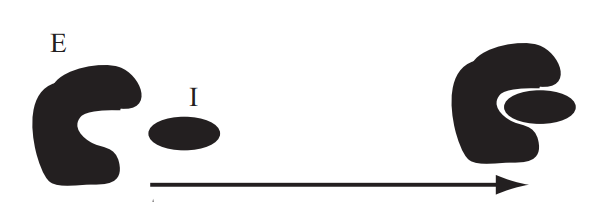
\includegraphics[scale=0.4]{enzymes.png}
\end{figure}

Let's assume there are two states $A$ and $B$.
We can assume that the potential $U_A$ is the interaction-free potential, while the potential $U_B$ the interactions between the enzyme and the inhibitor are taken into account.

$$U_A(\vec{r}_1, \dots, \vec{r}_n)\land U_{B}(\vec{r}_1, \dots, \vec{r}_N)$$

The potential $U_B$ would be the one used in the simulations, while in potential $U_A$ the only way in which the enzyme end the inhibitor could meet is through entropy, e.g. let the water molecules explore all of the configurations.

The free energy difference for state $A$ and state $B$ is:

$$\Delta A_{AB} = -kT\ln Q_B + kT\ln Q_A = -kT\ln\frac{Z_B}{Z_A}$$

Which can be written through the \textit{configurational partition function}, that is the partition function, but with the integration over the momenta already taken.

The two quantities:
$$Z_A = \int d^N\vec{r}e^{-\beta U_A(\vec{r}_1, \dots, \vec{r}_N)}\qquad Z_B = \int d^N\vec{r}e^{-\beta U_B(\vec{r}_1, \dots, \vec{r}_N)}$$

Are extremely difficult to compute. 
We would need to sum over all the possible states to get all of the contributions.
However, there a few tricks that can be used.

Let's write the partition function for state $B$:

$$Z_B = \int d^N\vec{r}e^{-\beta U_B(\vec{r}_1, \dots, \vec{r}_N)} = \int d^N\vec{r}e^{-\beta[U_B(\vec{r}_1, \dots, \vec{r}_N)-U_{A}(\vec{r}_1, \dots, \vec{r}_N)]}e^{-\beta U_A(\vec{r}_1, \dots, \vec{r}_N)}$$

In the second equality we just multiply by the Boltzmann factor for state A.
We can easily write the following equality:

$$\frac{Z_B}{Z_A} = \frac{1}{Z_A}\int d^N\vec{r}e^{-\beta[U_B(\vec{r}_1, \dots, \vec{r}_N)-U_{A}(\vec{r}_1, \dots, \vec{r}_N)]}e^{-\beta U_A(\vec{r}_1, \dots, \vec{r}_N)}$$

The difference in energy between the states is then:
$$\Delta A_{AB} = -kT\ln\frac{Z_B}{Z_A}\qquad\frac{Z_B}{Z_A} = \biggl\langle e^{-\beta[U_B(\vec{r}_1, \dots, \vec{r}_N)-U_A(\vec{r}_1, \dots, \vec{r}_N)]}\biggr\rangle_A$$

Free energy perturbation formula (Zwanzig, 1954):

$$\Delta A_{AB} = -kT\ln\biggl\langle e^{-\beta[U_B(\vec{r}_1, \dots, \vec{r}_N)-U_A(\vec{r}_1, \dots, \vec{r}_N)]}\biggr\rangle_A$$

The exponent is simply an energy difference, taken from the same force field, by switching off and on the interactions between the two objects of interest (defined by the potentials). 
The difficulty in using this equilibrium is that while sampling the canonical distribution for sate $A$, there's very little probability of finding an overlap between the two states.

In case of poor overlap we use the same formula as before, but applied to each step in this calculation:

$$\Delta A_{AB}=0kT\sum\limits_{\alpha=1}^{M-1}\ln\bigl\langle e^{-\beta\Delta U_{\alpha, \alpha+1}(\vec{r}_1, \dots,\vec{r})N}\bigr\rangle_\alpha$$

The average has to be calculated for every state $\alpha$.
This also means that each simulation is independent from each other (and can be run in parallel).

	\subsection{Adiabatic switching}
Instead of using a discretized version of the free energy perturbation, we can apply a switching function tot he two potentials.
The resulting potential is a combination of the potential describing state $A$ and the one describing state $B$:
	$$U(\vec{r}_1, \dots, \vec{r}_N, \lambda) \equiv f(\lambda)U_A(\vec{r}_1, \dots, \vec{r}_N)+g(\lambda)U_B(\vec{r}_1, \dots, \vec{r}_N)$$
	
	We can define the function $\lambda$ as:

	$$f(0) = 1, \quad f(1) = 0,\quad g(0) = 0, \quad g(1) = 1$$
	
	The partition function (from the canonical ensemble) now will depend on $\lambda$:

	$$Q(N, V, T, \lambda) = C_N\int d^N\vec{p}d^N\vec{r}e^{-\beta\biggl[\sum\limits_{i=1}^N\frac{\vec{p}_o^2}{2m_i}+U(\vec{r}_1, \dots, \vec{r}_N, \lambda)\biggr]}$$
Also the Helmholtz free energy will depend on $\lambda$:
	$$A(N, V, T, \lambda) = -kT\ln Q(N, V, T, \lambda)$$
	
	What if we take the derivative of the Helmoltz free energy wet $lambda$?
	The derivative is:

	$$\frac{\partial A}{\partial \lambda} = -\frac{kT}{Q}\frac{\partial Q}{\partial \lambda} = -\frac{kT}{Z}\frac{\partial Z}{\partial\lambda}$$
	
	Since $\lambda$ only appears in the potential and not on the kinetic energy, the derivative can be written as $-\frac{kT}{Z}\frac{\partial Z}{\partial\lambda}$.
	
	The derivative can be written in a better way:

	$$\frac{kT}{Z}\frac{\partial Z}{\partial \lambda} = \frac{kT}{Z}\frac{\partial}{\partial\lambda}\int d^N\vec{r}e^{-\beta U(\vec{r}_1, \dots, \vec{r}_N, \lambda)} = \frac{kT}{Z}\int d^{N}\vec{r}\biggl(-\beta\frac{\partial U}{\partial\lambda}\biggr)e^{-\beta U(\vec{r}_1, \dots, \vec{r}_N)} = -\biggl\langle\frac{\partial U}{\partial\lambda}\biggr\rangle$$

	At the end we get the derivative of $U$ wrt $\lambda$. One trivial function that satisfies the first relation would be, for example, a function that is $f = 1-\lambda$ and $g = \lambda$. 
	For such a  function, the adiabatic switching looks like the Zwanzig's procedure, but we can use any function.
	

	\subsection{Thermodynamics integration}

	The free energy difference between $A$ and $B$ can be defined as the formula below, using the result from the adiabatic switching:

	$$\Delta A_{AB} = \int_0^1\biggl(\frac{\partial A}{\partial \lambda}\biggr)d\lambda = \int_0^1\biggl\langle\frac{\partial U}{\partial\lambda}\biggr\rangle_\lambda d\lambda$$
	There are many ways in which integrals can be computed, e.g. \textit{Gaussian Quadrature}, which gives the best approximation for a small number of points.
	In this case, every value of $\lambda$ would be an independent run of a simulation, so many simulations can be run at the same time and use the found points to calculate the integral. 
	There's however another method: thermodynamic integration.
	The aim of the method is to make the region between $\lambda=0$ and $\lambda=1$ energetically unfavorable.
	Indeed, the difference between the energy of the states only depends on the initial and final state and does not depend on the route the system takes to make such a transition.
	\begin{figure}[H]
		\centering
		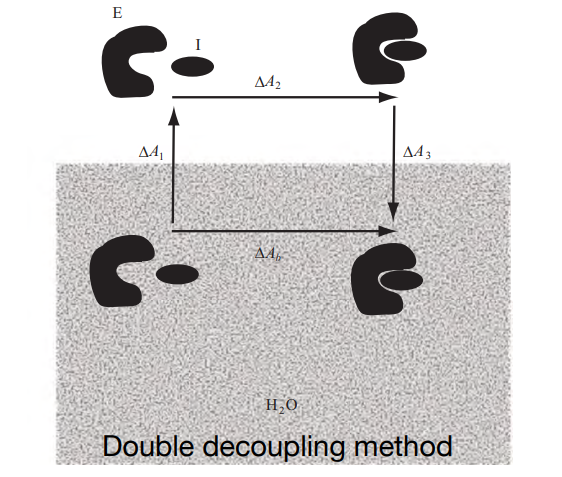
\includegraphics[scale=0.5]{ddm.png}
		\caption{Representation of two thermodynamic pathways for the calculation of the binding free energy of an enzyme E and inhibitor I. According the figure $\Delta A_b = \Delta A_1 + \Delta A_2 + \Delta A_3$}
		\label{fig:ddm}
	\end{figure}
	
	In the real case, some water molecules may affect the dynamics of the system and we cannot arbitrarily remove all the molecules of the solvent.
	
	\subsection{Adiabatic Free Energy Dynamics}
	There are several other methods to calculate the free energy difference.
	For the methods seen before, the difference between all of the states in the middle of the two states of interest have to be calculated.
	We would like instead to explore more the states $A$ and $B$.
	In Adiabatic Free Energy Dynamics, $\lambda$ becomes a variable in the hamiltonian (with associated momenta).

	$$\mathcal{H}_\lambda(\vec{r}, \lambda, \vec{p}, p_\lambda) = \frac{p_\lambda^2}{2m_\lambda} + \sum\limits_{i=1}^N\frac{\vec{p}_i^2}{2m_i} + U(\vec{r}_1, \dots, \vec{r}_N, \lambda)$$

	In the partition function, we integrate also over the values of $lambda$:
	$$Q(N, V, T) = \int dp_\lambda\int d^N\vec{p}\int_0^1d\lambda\int d^N\vec{r}e^{-\beta\mathcal{H}_\lambda(\vec{r},\lambda,\vec{p}, p_\lambda)}$$

	The probability distribution is $P(\lambda') = \langle\delta(\lambda-\lambda')\rangle$. 
	Once we have the probability distribution we can define the \textbf{free energy profile}: $A(\lambda') = -kT\ln P(\lambda')$. 
	This free energy profile would be negative only with very high value of $P(\lambda ')$, e.g. a deep well in the potential.
	
	$P(1)$ would be the partition function for state $B$, and $P(0)$ would be the partition function for state $A$:

	$$A(1) = A(0) = -kT\ln\frac{P(1)}{P(0)} = -kT\ln\frac{Q_B}{Q_A} = \Delta A_{AB}$$


	\begin{figure}[H]
		\centering
		\includegraphics[scale = 0.5]{adiabatic-free-energy-dynamics}
		\caption{\textbf{(a)} Free energy profiles. The solid line indicates switches
$f(\lambda) = (\lambda^2 - 1)^2$ and $g(\lambda) = ((\lambda - 1)^2 - 1)^2$, and the dashed line indicates $f(\lambda) = (\lambda^2 - 1)^4$ and $g(\lambda) = ((\lambda - 1)^2 - 1)^4$ . \textbf{(b)} Corresponding switch $f(\lambda)$.}
		\label{fig:adiabatic-free-energy-dynamics}
	\end{figure}

	In figure \ref{fig:adiabatic-free-energy-dynamics}(a) we can see the energy profiles for different functions. 
	The free energy difference is the same for the two methods, but the profile is very different.
	In the profile that displays a minimum, we expect to be spending more time away from the configurations of interest, in regions which are not physical. 
	In the second case, which shows a maximum point, the configurations in which we spend more time are the ones closer to $\lambda = 0$ and $\lambda = 1$. 
	
	If the system has a barrier $U^{\ddagger}$, the probability to cross a barrier $U^{\ddagger}$ is proportional to $e^{-\frac{U^{\ddagger}}{kT}}$.
	
	In Adiabatic free energy dynamics the idea is to raise the temperature of the $\lambda$ degree of freedom: $\biggl\langle\frac{p_\lambda^2}{2m_\lambda}\biggr\rangle = kT_\lambda$.
	The term $lambda$ is now very hot, more than the actual temperature at which we want to simulate the system.
	However, this makes $\lambda$ fluctuate a lot, which is not desirable, so we also increase its mass.
	This is called adiabatic decoupling: it increases $m_\lambda$ until the $\lambda$ degree of freedom is decoupled from all other degrees of freedom. 
	Now $\lambda$ is almost fixed:

	$$Z(\lambda, \beta) = \int d^N\vec{r}e^{-\beta U(\vec{r}, \lambda)}\qquad\text{ Correct if }\lambda\text{ is fixed}$$
	
	The temperature $\beta$ is the temperature at which we want to simulate the system.
	Because of decoupling, we assume that in the simulation there's enough time for the system to equilibrate and to explore all its possible conformations in a particular value of $\lambda$

	We can now define the\textbf{ potential of mean force} in $\lambda:-\frac{1}{\beta}\ln Z(\lambda, \beta)$.
	
	Because of adiabatic decoupling, $\lambda$ moves quasi-independently from the physical degrees of freedom in the potential of mean force, subject to an effective Hamiltonian:

	$$\mathcal{H}_{eff}(\lambda, p_\lambda) = \frac{p_\lambda^2}{2m_\lambda} -\frac{1}{\beta}\ln Z(\lambda, \beta)$$ 
	
	In this hamiltonian, the kinetic energy is thermostatted by $\lambda$ and the potential of mean force acts as a potential. 
	Notice that in this hamiltonian the potential depends on the temperature, which is usually not the case (this is the reason why it is an "effective" hamiltonian). 
	

	$\lambda$ is thermostatted at a temperature $T_\lambda>T$, hence the obtained canonical distribution ($adb$ because it is obtained through decoupling) is:

	$$P_{adb}(\lambda, p_\lambda, \beta, \beta_\lambda)\propto e^{-\beta_\lambda\mathcal{H}_{eff}(\lambda, p_\lambda)}$$
	
	If we want to obtain the probability distribution for $\lambda$ we need to integrate over $p_{lambda}$:

	$$\tilde{P}_{adb}(\lambda, \beta, \beta_\lambda) = \int dp_\lambda P_{adb}(\lambda, p_\lambda, \beta, \beta_\lambda)\propto e^{\beta_\lambda\ln \frac{Z(\lambda, \beta)}{\beta}} = [Z(\lambda, \beta)]^{\frac{\beta_\lambda}{\beta}}$$
	
	If we take the free energy profile for the probability distribution $[Z(\lambda, \beta)]^{\frac{\beta_\lambda}{\beta}}$:

	$$A(\lambda) = -kT_\lambda\ln\tilde{P}_{adb}(\lambda, \beta, \beta_\lambda) = -kT\ln Z(\lambda, \beta) + const$$

	And we get the free energy profile for the temperature at which we want to obtain the free energy difference, and not for the temperature used for the $\lambda$ degree of freedom. 

\section{Jarzynski's equality}
The free energy difference is called in called in this way because there exists the work-free energy inequality: $W_{AB}\ge \Delta A_{AB}$.
In every thermodynamic transformation, the work is equal to $\Delta A_{AB}$ only if the transformation is fully reversible.
To calculate the work, we need an estimator for it.
We want to obtain a quantity that is equal to the free energy difference, no matter which transformation is happening.
$W_{AB}$ is a thermodynamic quantity and can be expressed as a thermodynamic average:

$$W_{AB} = \langle\mathcal{W}_{AB}(x)\rangle$$

Initial distribution of microstates $x_0\in A$.
They can be all the microstates compatible with the conditions that define state $A$, e.g. state $A$ has its own temperature, so the microstates will be weighted by the Boltzmann factor (Canonical distribution).
The work $\mathcal{W}_{AB}(x_0)$ is a functional of the path $\mathcal{W}_{AB}[x_t] = \mathcal{W}_{AB}[x_t(x_0)] = \mathcal{W}_{AB}(x_0)$.
For each microstate, the system will evolve in a different path.

The thermodynamic value for the work is then:
$$W_{AB} = \langle\mathcal{W}_{AB}(x_0)\rangle_A=\frac{C_N}{Q_A(N, V, T)}\int dx_0e^{-\beta\mathcal{H}_A(x_0)}\mathcal{W}_{AB}(x_0)\ge \Delta A_{AB}$$

Jarzynski's theorem states that if instead of calculating the average over all initial conditions $\langle\mathcal{W}_{AB}(x_0)\rangle_A$ we calculate $\langle e^{-\beta\mathcal{W}_{AB}(x_0)}\rangle_A$ (it looks like a Boltzmann weight for the work estimator), then we get exactly $e^{-\beta\Delta A_{AB}}$, whatever the transformation is:

$$\langle e^{-\beta\mathcal{W}_{AB}(x_0)}\rangle_A = \frac{C_N}{Q_A(N, V, T)}\int dx_0e^{-\beta\mathcal{H}_A(x_0)}e^{-\beta\mathcal{W}_{AB}(x_0)} = e^{-\beta\Delta A_{AB}}$$

This equality also hold for irreversible transformations, that can be used to obtain quantities that describe states at equilibrium.
This has huge implication in computational and experimental physics: in practice it is very difficult to design an experiment with a reversible transformation, instead of an irreversible one.

\subsection{Jarzynski's equality Proof}
There are several proofs for Jarzynski's equality theorem, but we will only go through one.
Let's first define:
$$\Delta A_{AB} = -kT\ln\langle e^{-\beta\mathcal{W}_{AB}(x_0)}\rangle_A$$

And the time dependent Hamiltonian: 
$$\mathcal{H}(\vec{r}, \vec{p}, t) = \sum\limits_{i=1}^N\frac{\vec{p}_i^2}{2m_i} + U(\vec{r}, t)$$.

$$\frac{d\mathcal{H}}{dt} = \nabla_{x_t}\mathcal{H}\cdot\dot{x_t}+\frac{\partial\mathcal{H}}{\partial t}$$

$$\int_0^\tau\frac{d\mathcal{H}}{dt} = \underbrace{\int_0^\tau\nabla_{x_t}\mathcal{H}\cdot\dot{x}_tdt}_{\text{Heat}}+\underbrace{\int_0^\tau\frac{\partial\mathcal{H}}{\partial t}dt}_{\text{Work}}$$

If we use hamiltonian dynamics and there are no dissipative forces, the heat factor is equal to zero.
The formula above also represents the first law of thermodynamics.

The estimator for the work is $\mathcal{W}_{t'}(x_0)$:

$$\mathcal{W}_{t'}(x_0) = \int_0^{t'}\frac{\partial\mathcal{H}(x_t(x_0), t)}{\partial t}dt\qquad \mathcal{W}_{AB}(x_0) = \mathcal{W}_\tau(x_0)$$

Notice that if the hamiltonian is not explicitly time-dependent this would be null (no work is done in the system).

If hamilton's equations are used: $\nabla_{x_t}\mathcal{H}\cdot\dot{x}_t = 0\Rightarrow\frac{\partial\mathcal{H}}{\partial t} = \frac{d\mathcal{H}}{dt}$. 
Meaning, the partial time derivative can be substituted with the total time derivative and the integral can be calculated quite easily: 

$$W_{t'}(x_0) = \int_0^{t'}\frac{\partial\mathcal{H}(x_t(x_0),t)}{\partial t}dt = \int_0^{t'}\frac{d\mathcal{H}(x_t(x_0), t)}{dt}dt = \mathcal{H}(x_{t'}(x_0), t') - \mathcal{H}(x_0, 0)$$

Then the estimator is:
$$\mathcal{W}_{AB}(x_0) = \mathcal{W}_\tau(x_0) = \mathcal{H}(x_\tau(x_0), \tau)-\mathcal{H}(x_0,0)\qquad \mathcal{H}(x_0, 0) = \mathcal{H}_A(x_0)$$

Hence, if we take the average of the quantity $e^{-\beta\mathcal{W}_{AB}}$ by using the canonical ensemble for state $A$, then this is equal to the usual normalization constant divided by the partition function for state A, and the integral for all possible initial values for the compatible microstates:

$$\langle e^{-\beta\mathcal{W}_{AB}}\rangle_A = \frac{C_N}{Q_A(N, V, T)}\int dx_0e^{-\beta\mathcal{H}_A(x_0)}e^{-\beta[\mathcal{H}(x_\tau(x_0), \tau)-\mathcal{H}_A(x_0)]} = \frac{C_N}{Q_A(N, V, T)}\int dx_0e^{-\beta\mathcal{H}(x_\tau(x_0), \tau)}$$

We can cange of coordinates from $x_0$  to $x_\tau(x_0)$.
By Liouville's theorem $dx_\tau = dx_0$:

$$\langle e^{-\beta\mathcal{W}_{AB}}\rangle_A = \frac{C_N}{Q_A(N, V, T)}\int dx_\tau e^{-\beta\mathcal{H}_B(x_\tau)} = \frac{Q_B(N, V, T)}{Q_A(N, V, T)} = e^{-\beta\Delta A_{AB}}$$

$mathcal{H}$ at time $\tau$ is exactly the hamiltonian that described the system when the transformation is completed, so the hamiltonian that describes the system in state $B$.  
So $int dx_\tau e^{-\beta\mathcal{H}_B(x_\tau)}$, multiplied by the normalization constant, is exactly the partition function for state $B$.

\subsection{Application of Jarzynski's Equation}
Other versions of this proof are available, with thermostats for instance (see Tuckerman).
There are several applications: \textbf{pulling experiments}, mainly performed on small peptides.

\begin{figure}[H]
		\centering
		\includegraphics[scale=0.5]{pulling}
		\caption{Pulling experiment on a small peptide (Tuckerman, pg 328)}
		\label{fig:pulling}
	\end{figure}

The idea is to fix an end of the peptide and pull the other end, for example with optical tweezers in an experimental setting (shown in picture \ref{fig:pulling}.
Computationally, a time-dependent potential drives the end-to-end distance $|\vec{r}_1-\vec{r}_N|$ of a peptide away form its equilibrium value in the folded state:

$$U(\vec{r}_1, \dots, \vec{r}_N, t) = U_o(\vec{r}_1, \dots, \vec{r}_N) + \frac{1}{2}k\bigl(|\vec{r}_1-\vec{r}_N|-r_{eq}-vt\bigr)^2$$

We have a potential to describe the system and a harmonic term.
The pulling is performed at speed $v$.

Ensemble of initial conditions with different pulling rates.

$$\langle e^{-\beta\mathcal{W}_{AB}}\rangle_A = e^{-\beta\Delta A_{AB}}$$

The estimate gets better with the number of simulations performed. 

There are several problems, for example work values have a distribution $P(\mathcal{W}_\tau)$, as shown in figure \ref{fig:dist}.

\begin{figure}[H]
		\centering
		\includegraphics[scale=0.5]{dist}
		\caption{Shift in a Gaussian work distribution as a result of the multiplication by $exp(- \beta W_{\tau})$ for various values of $\tau$.}
		\label{fig:dist}
	\end{figure}	


We need to be very careful with defining the quantity 

$$\langle e^{-\beta\mathcal{W}_\tau}\rangle= \int\mathcal{W}_\tau P(\mathcal{W}_\tau)e^{-\beta\mathcal{W}_\tau}$$

There are however some tricks we can perform. For example if, and only if, we know $P(\mathcal{W}_\tau)$ is Gaussian:

$$\ln\langle e^{-\beta\mathcal{W}_\tau}\rangle\simeq-\beta\langle\mathcal{W}_\tau\rangle + \frac{\beta^2}{2}(\langle\mathcal{W}_\tau^2\rangle-\langle\mathcal{W}_\tau\rangle^2)$$

Also, we are not sure that at the end the system reaches equilibrium. 
If the force is too strong we are forcing the system out of equilibrium and we'll not reach convergence.

\section{Replica exchange Monte Carlo}
Replica ex change Monte Carlo is not a free energy calculation method.
However, in the case of proteins, the free energy profile is complicated, with a lot of free energy minima and maxima (\textbf{rough free energy profile}), like the one in figure \ref{fig:rough}.

\begin{figure}[H]
		\centering
		\includegraphics[scale=0.5]{rough}
		\caption{A two-dimensional rough potential energy surface.}
		\label{fig:rough}
	\end{figure}

The problem with exploring such complicated potentials is the high probability of gettin stuck in a minimum.
The way out of this is to build $M$ independent copies of a system: each replica is assigned a different value of some physical control variable or parameter.
The simulations are performed independently from each other, but at a certain time we try to go from one replica to another.
There are several methods to perform these "jumps".

	\subsection{Parallel tempering}
	$M$ independent copies of a system: $T_M>T_{M-1}>T_{M-2}>\cdots>T_1$, where $T_1$ is the temperature of the canonical distribution to be sampled.
	
	\begin{figure}[H]
		\centering
		\includegraphics[scale=0.5]{RE}
		\caption{Schematic of the parallel-tempering replica exchange Monte Carlo.}
		\label{fig:RE}
	\end{figure}
	
	At temperature $T_M$ we can sample everywhere, but every now and then we want to try to switch coordinates.
	
	Configuration of replicas $\vec{r}^{(1)}, \dots, \vec{r}^{(M)}$.
	Independent replicas: total probability distribution:

	$$F(\vec{r}^{(1)}, \dots, \vec{r}^{(M)}) = \prod\limits_{K=1}^Mf_K(\vec{r}^{(K)})\qquad f_K(\vec{r}^{(K)}) = \frac{e^{-\beta_K U(\vec{r}^{(K)})}}{Q(N ,V, T_K)}$$

	Select randomly two neighboring replicas and attempt replica exchange:

	$$(\vec{r}^{(K)}, \vec{r}^{(K+1)})\rightarrow (\tilde{\vec{r}}^{(K)}, \tilde{\vec{r}}^{(K+1)})\qquad\text{ with }\qquad \tilde{\vec{k}}^{(K+1)} = \vec{r}^{(K)}\land \tilde{\vec{r}}^{(K+1)}=\vec{r}^{(K)}$$

	Coordinates are merely exchanged:

	$$T(\tilde{\vec{r}}^{(K)}, \tilde{\vec{r}}^{(K+1)}|\vec{r}^{(K)}, \vec{r}^{(K+1)}) = T(\vec{r}^{(K)}, \vec{r}^{(K+1)}|\tilde{\vec{r}}^{(K)}, \tilde{\vec{r}}^{(K+1)})$$
	
	The $T$ is the trial probability for a move that takes the system from coordinates $vec{r}^{(K)}, \vec{r}^{(K+1)}$ to the coordinates $\vec{r}^{(K)}, \vec{r}^{(K+1)}$. 

	The acceptance probability is given by the metropolis rule:

	$$A(\tilde{\vec{r}}^{(K)}, \tilde{\vec{r}}^{(K+1)}|\vec{r}^{(K)}, \vec{r}^{(K+1)}) = A(\vec{r}^{(K+1)}, \vec{r}^{(K)} | \vec{r}^{(K)}, \vec{r}^{(K+1)})$$
	
	The probability for a new state is given by  $f_K(\vec{r}^{(K+1)})f_{K+1}*\vec{r}^{(K)}$. 
	
	$$A(\vec{r}^{(K+1)}, \vec{r}^{(K)} | \vec{r}^{(K)}, \vec{r}^{(K+1)}) = \min\biggl[1, \frac{f_K(\vec{r}^{(K+1)})f_{K+1}*\vec{r}^{(K)}}{f_K(\vec{r}^{(K)})f_{K+1}(\vec{r}^{(K+1)})}\biggr] = \min[1, e^{-\Delta_{K, K+1}}]$$

	$$\Delta_{K, K+1} = (\beta_k-\beta_{K+1})[U(\vec{r}^{(K+1)}) - U(\vec{r}^{(K)})]$$\footnote{In the Tuckerman these two terms have opposite sign.}
	
	Some switches of replicas can be done up high, meaning the system will \textit{percolate}, that will therefore go through barriers in this way.
	
	\subsection{Wang-Landau sampling}
	The Wang-Landau sampling is a clever way to build the partition function at any possible temperature by simply running a simulation: \textbf{iterative method}.

	The partition function can be derived by using Boltzmann weights and the densities of states (how many states are there at energy $E$): 
	$$Q(N, V, T) = \frac{1}{E_0}\int_0^{\infty}dEe^{-\beta E}\Omega(N, V, E)\Rightarrow Q(\beta) = \int_0^{\infty}dEe^{-\beta E}\Omega(E)$$
	
	The partition function becomes an integral over all values of energy of the function given by the Boltzmann factor and the density.
	
	The idea is to obtain directly $\Omega(E)$, the inverse of the probability of state $E$.
	Assign $\Omega(E)=1\forall E$ (discredited), meaning all energy values are equally probable (which is not really the case).
	Then a trial move is performed: $E_1\rightarrow E_2$ and it is accepted by the metropolis rule:

	$$A(E_2|E_1) = \min\biggl[1, \frac{\Omega(E_1)}{\Omega(E_2)}\biggr]$$

	After each move: $\Omega(E)\rightarrow \Omega(E)f\quad f>1$.
	If we visit one particular value of the energy, then the density of states for that value will increase.
	Thus meaning that the probability of visiting again that state will decrease.
	
	We can build the histogram $h(E)$ of visited states, that will become always more flat with time.
	Once $h(E)$ is flat enough a new value $f_{new} = \sqrt{f_{old}}$ is switched and the algorithms continue until convergence.
	There is no detailed balance due to $f$.
	
	
	
	
	
	
	
	
	
	
	
	
	
	
	

  % \graphicspath{{chapters/19/images/}}
\chapter{Rare events}

\section{Introduction}
Many observed transitions observed in biology could be considered rare events in the time scales of all atoms simulations.
This is because many processes require time-scales of seconds.

	\subsection{Rough free energy surfaces}
	The problem is that we have to deal with rough free energy surface with lots of local minima.
	Even in the case of \ref{fig:rough-free-energy-surfaces} there are $4$ local minima.
	Moreover the number of local minima which is exponential for proteins with respect to their size.

	\begin{figure}[H]
		\includegraphics[width=\textwidth]{rough-free-energy-surfaces}
		\caption{Rough free energy surfaces}
		\label{fig:rough-free-energy-surfaces}
	\end{figure}

	Because of this the problem of studying this transition is difficult.

	\subsection{Variables in rare events}
	Describing the free-energy surface is difficult because the energies surfaces is complex.
	The variables necessary to study these events can be called:

	\begin{multicols}{2}
		\begin{itemize}
			\item Reaction coordinates: how to describe a transition between states.
			\item Order parameters: they describe the transition between one energy minimum from another.
			\item COLVARs: collective variables.
		\end{itemize}
	\end{multicols}

\section{Reaction coordinates}
There might be several reaction coordinates and the first problem is how to choose them.
This is system dependent.
For example considering dissociation reactions $AB\rightarrow A+B$ a good reaction coordinate could be the distance between the centre of mass of the atoms $r = |\vec{r}_B-\vec{r}_A|$.
Considering a protein, describing the transition from folded to unfolded one global measure is the radius of gyration:

$$R_G = \sqrt{\frac{1}{N_b}\sum\limits_{i=1}^{N_b}\biggl(\vec{r}_i-\frac{1}{N_b}\sum\limits_{j=1}^{N_b}\vec{r}_j\biggr)^2}$$

This gives a measure of how compact a protein is.
This is a good measure of foldedness in case of globular proteins, but this is not true for all proteins.
Another example is considering the number of hydrogen bonds between two elements of length $d_0$ between $n_O$ oxygens and $n_H$ hydrogens a good measure is:

$$N_H = \sum\limits_{i=1}^{n_O}\sum\limits_{j=1}^{n_H}\frac{1-\biggl[\frac{\vec{r}_i-\vec{r}_j}{d_0}\biggr]^6}{1-\biggl[\frac{\vec{r}_i-\vec{r}_j}{d_0}\biggr]^{12}}$$

The objective is to obtain a single coordinate from the Cartesian coordinates as to understand the process that is happening.
After having obtained the reaction coordinates the aim is to obtain the probability distribution function of a subset of $n$ reaction coordinates of interest $q_\alpha= f_\alpha(\vec{r}_1, \dots, \vec{r}_N)$ with $\alpha = 1, \dots, n$ which will not be in general factorized and can be written as:

$$P(s_1, \dots, s_n) = \frac{C_N}{Q(N, V, T)}\int d^N\vec{p}d^B\vec{r}e^{-\beta\mathcal{H}(\vec{r}, \vec{p})}\prod\limits_{\alpha=1}^n\delta(f_\alpha(\vec{r}_1, \dots, \vec{r}_N)-s_\alpha)$$
For the canonical ensemble.
Once the probability is obtained the free energy hypersurface can be obtained directly:

$$A(s_1, \dots, s_n) = -fT\ln P(s_1, \dots, s_n)$$

If the right reaction coordinates are not chosen then free energy profiles might not be describing the system correctly.
To judge the quality of the chosen reaction coordinates is the committor distribution, an extremely expensive process but that can be worthwhile.

	\subsection{Blue moon ensemble}
	One method to obtain rare events is the blue moon ensemble.
	When choosing a reaction coordinate the objective is to force a transition between states.
	The idea behind the blue moon ensemble is that considering for semplicity a single reaction coordinate $q_1 = f_1(\vec{r}_1, \dots, \vec{r}_N)$, its probability distribution is:

	$$P(s) = \frac{C_N}{Q(N, V, T)}\int d^N\vec{p}d^N\vec{r}e^{-\beta\mathcal{H}(\vec{r}, \vec{p})}\delta(f_1(\vec{r}_1, \dots, \vec{r}_N)-s)$$

	And the free energy profile:

	$$A(s) = -kT\ln P(s)$$

	A holonomic constraint is introduced $\sigma(\vec{r}_1, \dots, \vec{r}_N) = f_1(\vec{r}_1, \dots, \vec{r}_N)-s$.
	Then the sampling happens at that given value.
	So that the reaction coordinates assume a given set of values.
	Use this constraint to drive the reaction coordinate from an initial value $s^{(i)}$ to a final value $s^{(f)}$.
	The blue moon ensemble yields $\frac{dA}{ds} = -\frac{kT}{P(s)}\frac{dP}{ds}$.
	From this quantity then the free energy at any value of reaction coordinate $q$ can be reconstructed knowing the initial value.
	The free energy difference can be also computed:

	$$A(q) = A(s^{(i)}) + \int_{s^{(i)}}^q\frac{dA}{ds}ds\qquad \Delta A = \int_{s^{(i)}}^{s^{(f)}}\frac{dA}{ds}ds$$

	The probability distribution for the reaction coordinate $s$ is given by:

	$$P(s) = \frac{C_N}{Q(N, V, T)}\int d^N\vec{p}d^N\vec{r}e^{-\beta\mathcal{H}(\vec{r}, \vec{p})}\delta(f_1(\vec{r}_1, \dots, \vec{r}_N)-s) = \langle\delta(f_1(\vec{r}_1, \dots, \vec{r}_N)-s)\rangle$$

	The quantity obtained from the simulation:

	$$\frac{1}{P(s)}\frac{dP}{ds} = \frac{C_N}{Q(N, V, T)}\frac{\int d^N\vec{p}d^N\vec{r}e^{-\beta\mathcal{H}(\vec{r}, \vec{p})}\frac{\partial\delta(f_1(\vec{r})-s)}{\partial s}}{\langle\delta(f_1(\vec{r})-s)\rangle}$$

	Introduce $3N$ generalized coordinates $q_\alpha = f_\alpha(\vec{r}_1, \dots, \vec{r}_N)$ so that $q_1$ is the reaction coordinate of interest and their conjugate momenta $p_\alpha$,
	The transformation is canonical, hence the Jacobian is one: $d^N\vec{p}d^N\vec{r} = d^{3N}pd^{3N}q$, so the quantity is:

	$$\frac{1}{P(s)}\frac{dP}{ds} = \frac{C_N}{Q(N, V, T)}\frac{\int d^{3N}pd^{3N}qe^{-\beta\tilde{\mathcal{H}}(q, p)}\frac{\partial\delta(q_1-s)}{\partial s}}{\langle\delta(q-s)\rangle}$$

	However $\frac{\partial}{\partial s}\delta(q_1-s) = -\frac{\partial}{\partial q_1}\delta(q_1-s)$ substituting in the integral and integrating by parts:

	\begin{align*}
		\frac{1}{P(s)}\frac{dP}{ds} &=-\frac{\beta C_N}{Q(N, V, T)}\frac{\int d^{3N}pd^{3n}q\frac{\partial\tilde{\mathcal{H}}}{\partial q_1}e^{-\beta\tilde{\mathcal{H}}(q, p)}\delta(q_1-s)}{\langle\delta(q_1-s)\rangle} = \\
																&= -\frac{\beta}{\langle\delta(q_1-s)\rangle}\biggl\langle\frac{\partial\tilde{\mathcal{H}}}{\partial q_1}\delta(q_1-s)\biggr\rangle \equiv -\beta\biggl\langle\frac{\partial\tilde{\mathcal{H}}}{\partial q_1}\biggr\rangle^{cond}
	\end{align*}

	In this way everything can be expressed in term of the conditional average subject to the condition that $q_1=s$.
	The simulation is run and the average value of the quantity is taken thanks to the holonomic constraint.
	This is measured with different initial values so that in the end the free energy as a function of the reaction coordinate:

	$$A(q) = A(s^{(i)}) + \int_{s^{(i)}}^q\biggl\langle\frac{\partial\tilde{\mathcal{H}}}{\partial q_1}\biggr\rangle^{cond}_sds$$

	\subsection{Umbrella sampling}
	Umbrella sampling substitutes the rigid holonomic contraints of blue moon sampling with a more flexible harmonic restraint.
	An extra potential or bias potential is introduced such that the reaction coordinates are constraint to be close to the value $s_k$:

	$$W_k(f_1(\vec{r}_1, \dots, \vec{r}_N), s_k) = \frac{1}{k}[f_1(\vec{r}_1, \dots, \vec{r}_N)-s_k]^2$$

	The probability distribution for $s$ is biased to be close to $s_k$.
	The biased probability distributions obtained will be:

	$$P(s, s^{(k)}), k= 1, \dots, n,\qquad s^{(1)}=s^{(i)}, s^{(n)}=s^{(f)}$$

	From this a collection of biased probability distribution, one for each value of $k$ is obtained.
	This probability distribution should be used to reconstruct the real one.
	To do so the weighted histogram analysis method is used.

	\subsection{WHAM}
	The weighted histogram analysis method is used to obtain from the collection of biased probability distribution obtained from umbrella sampling the real one.
	For each of the $k$ biased probability distributions generated by umbrella sampling:

	$$\tilde{P}(q, s^{(k)}) = e^{\beta A_k}\int d^N\vec{r}e^{-\beta U(\vec{r})}e^{-\beta W_k(f_1(\vec{r}), s^{(k)})}\delta(f_1(\vec{r})-q)$$

	Where $e^{\beta A_k}$ is the normalization factor and $A_k$ is the free energy associated with the biasing potential apart from constants so that:

	$$e^{-\beta A_k} = \int d^N\vec{r}e^{-\beta U(\vec{r})}e^{-\beta W_k(f_1(\vec{r}), s^{(k)})}=e^{-\beta A_0}\biggl\langle e^{-\beta W_k(f_1(\vec{r}), s^{(k)})}\biggr\rangle$$

	The average is taken with respect to the unbiased potential:

	$$e^{-\beta A_0} = \int d^N\vec{r}e^{-\beta U(\vec{r})}$$

	To unbiase the probability distributions the Boltzmann factor is introduced:

	$$P_k(q) = e^{-\beta(A_k-A_0)\beta W_k(q, s^{(k)})}\tilde{P}(q, s^{(k)})$$

	A collection of $n$ unbiased probability distribution is obtained that describe a single region of the possible values of the reaction coordinates.
	To reconstruct the full probability distribution the objective is to combine them into a single one.
	To do that these distribution are combined with weights $C_k$ such that $\sum\limits_{k=1}^n C_k=1$, so the total probability distribution is:

	$$P(q) = \sum\limits_{k=1}^n C_k(q)P_k(q) = \sum\limits_{k=1}^nC_k(q)e^{-\beta(A_k-A_0)}e^{\beta W_k(q, s^{(k)})}\tilde{P}(q, s^{(k)})$$

	The values of $C_k$ have to be obtained using a criterion, so the statistical error in the distribution generated by the WHAM procedure is minimized.
	To obtain the biased probability distribution let $\tilde{H}_k(q)$ be the biased histogram obtained from each molecular dynamics or Monte Carlo simulation.
	The system will be in that position from a given number of frame.
	The estimate for the biased distributions is:

	$$\tilde{P}(q, s^{(k)}) \approx\frac{1}{n_k\Delta q}\tilde{H}_k(q)$$

	Where:

	\begin{multicols}{2}
		\begin{itemize}
			\item $n_k$ is the number of frames in an umbrella window.
			\item $\Delta q$ takes into account that the possible value of the reaction coordinate are in bins.
		\end{itemize}
	\end{multicols}

	The statistical error for the umbrella window is

	$$\tilde{\sigma}^2_k = \frac{\epsilon_k(q)\tilde{H}_k(q)}{n_k\Delta q}$$

	Where $\epsilon_k$ is a given factor.
	This is because since there are a number of occurrences of these stochastic process the number of occurrences is a Poisson process.
	The error in $P_k(q)$ (the unbiased probability distribution) is given by applying the square of the unbiasing  factor:

	$$\sigma_k^2 = e^{-2\beta(A_k-A_0)}e^{2\beta W_k(q, s^{(k)})}\tilde{\sigma}_k^2$$

	The total error will be:

	$$\sigma^2 = \sum\limits_{k=1}^nC_k^2(q)\sigma_k^2$$

	To minimize the total statistical error considering the condition that the sum over the $C_k$ is equal to $1$.
	To do so Lagrange multipliers are used.
	Then the function to minimize is:

	$$\Sigma^2=\sum\limits_{k=1}^nC_k^2(q)e^{-2\beta (A_k-A_0)}e^{w\beta W_k(q, s^{(k)})}\frac{\epsilon_k(q)\tilde{H}_k(q)}{n_k\Delta q}-\lambda\left(\sum\limits_{k=1}^nC_k(q)-1\right)$$

	The unknowns are $C_k$ and $\lambda$, so now to minimize:

	$$\frac{\partial\Sigma^2}{\partial C_k(q)} = 0\Rightarrow C_k(q) = \frac{\lambda n_k\Delta q}{2\epsilon_k(q)\tilde{H}_k(q)e^{-2\beta(A_k-A_0)}e^{2\beta W_k(q, s^{(k)})}}$$

	All the $C_k$ depends on $\lambda$.
	$\lambda$ is unknown and to determine it the normalization condition is used:

	$$\lambda = \frac{1}{\sum\limits_{k=1}^n\frac{n_k\Delta q}{2\epsilon_k(q)\tilde{H}_k(q)e^{-2\beta(A_k-A_0)}e^{2\beta W_k(q, s^{(k)})}}}$$

	The solution for $C_k$ is obtained:

	$$C_k(q) =\frac{n_kl\bigl[\epsilon_k(q)\tilde{H}_k(q)e^{-2\beta(A_k-A_0)}e^{2\beta W_k(q, s^{(k)})}\bigr]}{\sum\limits_{j=1}^n n_jl\bigl[\epsilon_j(q)\tilde{H}_j(q)e^{-2\beta(A_j-A_0)}e^{2\beta W_k(q, s^{(j)})}\bigr]}$$

	Considering the following simplifying assumption that they need to be checked in the system:

	\begin{multicols}{2}
		\begin{itemize}
			\item $\epsilon_k(q)$ is the same for all umbrella windows.
				This does not imply that all the umbrella windows are of the same size, but that the quality of sampling is the same for all of them.
			\item $\tilde{H}_k(q)\propto e^{\beta(A_k-A_0)}e^{-\beta W_k(q, s^{(k)})}P(q)$.
				The histogram of the probability distribution is proportional to the real distribution biased by the two factors.
		\end{itemize}
	\end{multicols}

	Assuming these $C_k$ can be simplified into:

	$$C_k(q) = \frac{n_ke^{\beta A_k}e^{-\beta W_k(q, s^{(k)})}}{\sum\limits_{j=1}^nn_je^{\beta A_j}e^{-\beta W_j(q, s^{(j)})}}$$

	Using this formula the full probability distribution will be:

	$$P(q) = \sum\limits_{k=1}^nC_k(q)P_k(q) = \frac{\sum\limits_{k=1}^nn_k\tilde{P}(q, s^{(k)})}{\sum\limits_{k=1}^nn_ke^{\beta(A_k-A_0)}e^{-\beta W_k(q, s^{(k)})}}$$

	However:

	$$e^{\beta(A_k-A_0)} = \int dq P(q)e^{-\beta W_k(q, s^{(k)})}$$

	These two equations are self consistent because one depends on the other, so the algorithm starts with a guess for $A_k$ and iterates until convergence.

	\subsection{Wang-Landau sampling}
	In the Wang-Landau approach the density of states were the objective with a Monte Carlo simulation.
	After devising some moves they where accepted with probability:

	$$A(\vec{r}_2|\vec{r}_1) = \min\biggl[1, \frac{\Omega(E_1)}{\Omega(E_2)}]\biggr]$$

	With scaling factor $f$ to scale the density of state each time one state was visited.
	The same can be extended to reaction coordinates: generate a function $g(s)$ that approaches the probability distribution $P(s)$.
	Start $g(s)=1$ and $h(s) = \ln g(s) = 0$ everywhere, then the same procedure is performed: a move is generated and accepted with:

	$$A(\vec{r}_2|\vec{r}_1) = \min\biggl[1, \frac{e^{-\beta U(\vec{r}_2)}}{e^{-\beta U(\vec{r}_1)}}\frac{g(s_1)}{g(s_2)}\biggr] = \min\biggl[1, \frac{e^{-\beta U(\vec{r}_2)}}{e^{-\beta U(\vec{r}_1)}}\frac{e^{-h(s_1)}}{e^{-h(s_2)}}\biggr]$$

	Every time a new value of $s$ is visited $h$ is updated by adding a factor $\alpha$:

	$$h(s_2) \rightarrow h(s_2) + \alpha \Leftrightarrow g(s_2)\rightarrow fg(s_2)\qquad \alpha = \ln f$$

	Iterate until the histogram $H(s)$ becomes flat, then reduce $f$ and repeat until convergence.
	When convergence is reached $P$ is obtained.
	Its efficiency and accuracy depends on the choice of reaction coordinates.

  % \graphicspath{{chapters/20/images/}}
\chapter{Advanced methods}

\section{Adiabatic dynamics}
In the free energy adiabatic dynamics the idea is to obtain the free energy hypersurface as a function of some reaction coordinates.
Let's assume the reaction coordinates $n<3N$ reaction coordinates with generalized coordinates $q_\alpha$: the interest is in the free energy hypersurface $A(q_1, \dots, q_n)$.
The partition function is defined, in the case of the canonica ensemble, as:

$$Q(N, V, T) = C_N\int d^N\vec{p}d^N\vec{r}e^{-\beta\biggl[\sum\limits_{i=1}^N\frac{\vec{p}_i^2}{2m_i}+U(\vec{r}_1, \dots, \vec{r}_N)\biggr]}$$

Transformation to generalized coordinates $q_\alpha = f_\alpha(\vec{r}_1, \dots, \vec{r}_n)$ only for the configurational part, leaving momenta unchanged:

$$Q(N, V, T) = C_n\int d^N\vec{p}d^{3N}qe^{-\beta\biggl[\sum\limits_{i=1}^N\frac{\vec{p}_i^2}{2m_i} + \tilde{V}(q_1, \dots, q_{3N}, \beta)\biggr]}$$

Where, considering the Jacobian of the transformation:

$$\tilde{V}(q_1, \dots, q_{3N}, \beta) = \tilde{U}(q_1, \dots, q_{3N}) - kT\ln J(q_1, \dots, q_{3N})$$

This is a function of all of the $3N$ coordinates.
This term looks like a potential in term with the generalized coordinates and the Jacobian.
In this term the potential is temperature dependent.
This is because $\tilde{V}$ has $\beta$ as a temperature parameters.
Using the Hamiltonian in the transformation during the simulation the canonical distribution is being sampled.
So consider the temperature dependent potential included into this fake Hamiltonian:

$$\tilde{\mathcal{H}}(q, \vec{p}, \beta) = \sum\limits_{i=1}^N\frac{\vec{p}_i^2}{2m_i}+\tilde{V}(q_1, \dots, q_{3N}, \beta) = \sum\limits_{i=1}^N\frac{\vec{p}_i^2}{2m_i}+\tilde{U}(q_1, \dots, q_{3N})-kT\ln J(q_1, \dots, q_{3N})$$

To conjugate the momenta to the velocities they need to be renamed.
This is not the original Hamiltonian but can be used as a Hamiltonian.
Renaming the momenta:

$$\tilde{H}(q, p, \beta) = \sum\limits_{\alpha=1}^{3N}\frac{p_\alpha^2}{2m'_\alpha}+ \tilde{V}(q_1, \dots, q_{3N}, \beta)$$

Where $m'_\alpha$ is a fictitious mass defined during the simulation.
As in adiabatic free energy dynamics the first $n$ variables are thermostatted as a temperature $T_q\gg T$ with their masses increased so to adiabatically decouple them from the others.
So the system should be have enough time to equilibrate for each variable.

	\subsection{TAMD}
	The previous idea can be implemented as TAMD (temperature accelerated molecular dynamics).
	Using the Hamiltonian with the renamed momenta:

	$$\tilde{H}(q, p, \beta) = \sum\limits_{\alpha=1}^{3N}\frac{p_\alpha^2}{2m'_\alpha} + \tilde{V}(q_1, \dots, q_{3N}, \beta)$$

	So that the differential equation to update positions:

	$$\dot{q}_\alpha = \frac{p_\alpha}{m'_\alpha}$$

	And momenta, where they are coupled with the thermostat variables needed to couple them to the Nos\`e-Hoover chain:

	$$\dot{p}_\alpha = -\frac{\partial\tilde{V}}{\partial q_\alpha} - \frac{p_{\eta_1}}{Q_1}p_\alpha\quad \alpha= 1, \dots, n\qquad\dot{p}_\alpha = -\frac{\partial\tilde{V}}{\partial q_\alpha}-\frac{p_{\eta_e}}{Q_2}p_\alpha\quad \alpha = n_1, \dots, 3N$$

	Then the variable for the thermostats:

	$$\dot{\eta}_j = \frac{p_{\eta_j}}{Q_j}$$

	Then the thermostat variable for the first $n$ generalized coordinates with $T_q$ higher tan $T$, while the other are coupled for the temperature $T$.

	$$\dot{p}_{\eta_1} = \sum\limits_{\alpha=1}^n\frac{p_\alpha^2}{2m'_\alpha}-nkT_q\qquad \dot{p}_{\epsilon_2} = \sum\limits_{\alpha=n+1}^{3N}\frac{p_\alpha^2}{2m'_\alpha}-(3N-n)kT$$

	It is possible to show that $A(q_1, \dots, q_n) = -kT_q\ln P_{adb}(q_1, \dots, q_n) + const$.
	So the free energy profile obtained by reconstructing the probability distribution for these $n$ generalized coordinate is equal to the one obtained for the energy profile at temperature $T$ in which the interest is in.
	An example can be seen in \ref{fig:tamd}, where it can be seen how the free energy profile using the bare potential is difficult to reconstruct the true analytical free energy.
	The others refers to TAMD and it can be seen how the mass associated to the reaction coordinate is much more the free energy profile is reconstructed well.
	This is because only in this case the system has enough time to explore the space at that value.

	\begin{figure}[H]
		\includegraphics[width=\textwidth]{tamd}
		\caption{TAMD}
		\label{fig:tamd}
	\end{figure}

\section{Metadynamics}
The objective is to reconstruct a probability for a set of reaction coordinates $s_1, \dots, s_n$ and the objective is to obtain the ensemble average for a function of reaction coordinates:

$$P(s_1, \dots, s_n) = \biggl\langle\prod\limits_{\alpha=1}^n\delta(f_\alpha(\vec{r}_1, \dots, \vec{r}_N)-s_\alpha)\biggr\rangle$$

Replacing phase space average with a time average over a trajectory.
This can be done only if the trajectory is ergodic:

$$P(s_1, \dots, s_n) = \lim\limits_{\mathcal{T}\rightarrow\infty}\frac{1}{\mathcal{T}}\int_0^{\mathcal{T}} dt\prod\limits_{\alpha=1}^n\delta(f_\alpha(\vec{r}_1, \dots, \vec{r}_N)-s_\alpha)$$

Where $\mathcal{T}$ is time.
However considering the following property of the delta function:

$$\delta(x-\alpha) = \lim\limits_{\sigma\rightarrow 0}\frac{1}{\sqrt{2\pi\sigma^2}}e^{-\frac{(x-\alpha)^2}{2\sigma^2}}$$

So adding this property to the probability distribution:

$$P(s_1, \dots, s_n) = \lim\limits_{\mathcal{T}\rightarrow\infty}\lim\limits_{\Delta s\rightarrow 0}\frac{1}{\mathcal{T}}\frac{1}{\sqrt{2\pi\Delta s^2}}\int_0^{\mathcal{T}}dt\prod\limits_{\alpha=1}^ne^{-\frac{(s_\alpha-f_\alpha(\vec{r}_1(t), \dots, \vec{r}_N(t)))^2}{2\Delta s^2}}$$

This looks like adding to the probability a factor similar to the Boltzmann factor and related to it because it looks like a Gaussian.
It looks like a Gaussian is added every time a value for a reaction coordinate $\alpha$ is visited so that the system will be forced to go somewhere else.
Building up these Gaussian potential they can be used as a bias potential:

$$U_G(\vec{r}_1, \dots, \vec{r}_N, t) = W\sum\limits_{t - \tau_G, 2\tau_G, \dots}e^{-\sum\limits_{\alpha=1}^n\frac{(f_\alpha(\vec{r})-f_\alpha(\vec{r}_G(t)))^2}{2\Delta s^2}}$$

This Gaussian potential is added at every $\tau_G$, the conformation already visited will be less favoured and the system will go somewhere else.
Taking all the Gaussian added this amount to summing over all the Gaussian it is the negative of the free-energy profiles, so keeping track of the added Gaussians, their sum is minus the free energy profile.
This is done only when the free diffusion of the system is observed, meaning that the algorithm has reached convergence.
Judging convergence is not easy for metadynamics.
In principle it is continued until free diffusion is observed for a number of times.
Another issue is that every time energy is being added to the system, which might cause problem.
For example in a membrane it would cause membrane disruption.

\section{Transition path ensemble}
In many situations the interest is in reconstructing a path for a transition going from state $A$ to state $B$.
Assume that by some method a pathway to go from state $A$ to state $B$ is obtained.

\begin{figure}[H]
	\includegraphics[width=\textwidth]{transition-path-ensemble}
	\caption{Transition path ensemble}
	\label{fig:transition-path-ensemble}
\end{figure}

To obtain the most probable path the transition path ensemble has to be introduced.
In order to reconstruct one point of the pathway in molecular dynamics Trotter factorization is applied:

$$x_{(k+1)\Delta t} = e^{iL_2\frac{\Delta t}{2}}e^{iL_1\Delta t}e^{iL_2\frac{\Delta t}{2}}x_{k\Delta t}\equiv\phi_{\Delta t}(x_{k\Delta t})$$

Considering in term of Monte Carlo moves instead:

$$T(x_{(k+1)\Delta t}|x_{k\Delta t}) = \delta(x_{(k+1)\Delta t}-\phi_{\Delta t}(x_{k_{\Delta t}}))$$

Assigning a weight to a single trajectory:

$$\mathcal{P}[X(\mathcal{T})] = f(x_0)\prod\limits_{k=0}^{n-1}T(x_{(k+1)\Delta t}|x_{k\Delta t})\qquad f(x_0) = \frac{e^{-\beta\mathcal{H}(x_0)}}{Q(N, V, T)}$$

This probability is given by starting from starting in $x_0$, which depends on the canonical distribution.
So $\mathcal{P}$ is the probability associated with a single trajectory.

$$\mathcal{P}[X(\mathcal{T})] = f(x_0)\prod\limits_{k=0}^{n-1}T(x_{(k+1)\Delta t}|x_{k\Delta t})$$


Defining the probability of a path $X$ going from $A$ to $B$ multiplies the probability associated for the path $X$ multiplied by $h_A$ and $h_B$, meaning that the starting point should be in the basin of state $A$ and the final point in the basin of state $B$, they are either $0$ or $1$.

$$\mathcal{P}_{AB}[X(\mathcal{T})] = \frac{1}{\mathcal{F}_{AB}(\mathcal{T})}h_A(x_0)\mathcal{P}[X(\mathcal{T})]h_B(x_{n\Delta t})$$

And $\mathcal{F}_{AB}$ is a normalization constant.

$$F_{AB}(\mathcal{T}) = \int dx_0\cdots dx_{n\Delta t}h_a(x_0)\mathcal{P}[X(\mathcal{T})]h_B(x_{n\Delta t})$$

For deterministic molecular dynamics trajectories:

\begin{align*}
	\mathcal{F}_{AB}(\mathcal{T}) &= \int dx_0\cdots dx_{n\Delta t}h_A(x_0)f(x_0)\prod\limits_{k=1}^{n-1}\delta(x_{(k+1)\Delta t}-\phi_{\Delta t}(x_{k\Delta t}))h_B(x_{n\Delta t}) = \\
																&=\int dx_0h_A(x_0)f(x_0)h_B(x_{n\Delta t}(x_0))
\end{align*}

	\subsection{Transition path sampling}
	Following the same method in Monte Carlo methods and Metropolis algorithm, introduce $\mathcal{R}_{AB}[X(\mathcal{T})|Y(\mathcal{T})]$, the conditional probability to generate a trajectory $X(\mathcal{T})$ starting from $Y(\mathcal{T})$.
	Considering the detailed balance condition:

	$$\mathcal{R}_{AB}[X(\mathcal{T})|Y(\mathcal{T})]\mathcal{P}_{AB}[Y(\mathcal{T})] = \mathcal{R}_{AB}[Y(\mathcal{T})|X(\mathcal{T})]\mathcal{P}_{AB}[X(\mathcal{T})]$$

	Splitting the conditional probabilities in two: one of generating the move and the other the probability to accept the move.

	$$\mathcal{R}_{AB}[X(\mathcal{T})|Y(\mathcal{T})] = \Lambda_{AB}[X(\mathcal{T})|Y(\mathcal{T})]\mathcal{T}_{AB}[X(\mathcal{T})|Y(\mathcal{T})]$$

	So now the acceptance probability can be written as:

	$$\Lambda_{AB}[X(\mathcal{T})|Y(\mathcal{T})] = \min\biggl[1, \frac{\mathcal{T}_{AB}[Y(\mathcal{T})|X(\mathcal{T})]\mathcal{P}_{AB}[X(\mathcal{T})]}{\mathcal{T}_{AB}[X(\mathcal{T})|Y(\mathcal{T})]\mathcal{P}_{AB}[Y(\mathcal{T})]}\biggr]$$

	In order to generate a move from $Y$ to $X$, it is assumed that $Y[\mathcal{T}]$ is a proper trajectory from $A$ to $B$, hence $h_A(y_0) = 1$ and $h_b(y_{n\Delta t}) = 1$.
	This means that the trajectory starts at $A$ and ends at $B$.
	Now a shooting move is performed: assuming that all the trajectories $Y$ start from state $A$ and end up in state $B$, then the only thing to check is the fact that the new trajectory starts at state $A$ and ends in state $B$:

	$$\Lambda_{AB}[X(\mathcal{T})|Y(\mathcal{T})] = h_A(x_0)h_B(x_{n\Delta t})\min\biggl[1, \frac{\mathcal{T}_{AB}[Y(\mathcal{T})|X(\mathcal{T})]\mathcal{P}_{AB}[X(\mathcal{T})]}{\mathcal{T}_{AB}[X(\mathcal{T})|Y(\mathcal{T})]\mathcal{P}_{AB}[Y(\mathcal{T})]}\biggr]$$

	\begin{figure}[H]
		\includegraphics[width=\textwidth]{transition-path-sampling}
		\caption{Shooting move}
		\label{fig:shooting-move}
	\end{figure}

	Assuming that $Y$ is a given trajectory and starting from a random point $y_{i\Delta t}$ in $Y$, starting from the point the momenta are regenerated so there is a new position in the system $x_{j\Delta t}$.
	With this coordinate and momenta it is integrated forward and backward in time.
	Now if integrating backward it is ended in $A$ and forward in $B$.
	If integrating forward going back to state $A$, this move has to be rejected because this new path does not start from state $A$ and ends up in state $B$.
	In the first case the move is accepted.
	In this way new pathways starting from a reasonable one can be generated, exploring the ensemble associated to the transition paths.
	$\tau(x_{j\Delta t}|y_{j\Delta t})$ is the rule to generate the shooting point.
	So a randomly chosen $y$ point in time, so the coordinates are not changed but the momenta are generated from a Boltzmann distribution.
	Then the probability to generate path $X$ to path $Y$ it the product of the probability of generate the point, the probability to shoot forward in time and the probability to shoot backward in time:

	$$\mathcal{T}_{AB}[X(\mathcal{T})|Y(\mathcal{T})] = \tau(x_{j\Delta t}|y_{j\Delta t})\biggl[\prod\limits_{k=j}^{n-1}T(x_{(k+1)\Delta t}|x_{k\Delta t})\biggr]\biggl[\prod\limits_{k=1}^jT(x_{(k-1)\Delta t}|x_{k\Delta t})\biggr]$$

	Using a deterministic rule the $T$ becomes delta functions.
	Looking at the acceptance probability, making explicit the $\mathcal{T}$s it can be seen how the forward part can be simplified and assuming that $T$ is symmetric another simplification can be made.

	\begin{align*}
		\Lambda_{AB}[X(\mathcal{T})|Y(\mathcal{T})] &= h_A(x_0)h_B(x_{n\Delta t})\min\biggl[1, \frac{\mathcal{T}_{AB}[Y(\mathcal{T})|X(\mathcal{T})]\mathcal{P}_{AB}[X(\mathcal{T})]}{\mathcal{T}_{AB}[X(\mathcal{T})|Y(\mathcal{T})]\mathcal{P}_{AB}[Y(\mathcal{T})]}\biggr] = \\
																								&= h_A(x_0)h_B(x_{n\Delta t})\min\biggl[1, \frac{f(x_0)}{f(y_0)}\biggl(\prod\limits_{k=0}^{n-1}\frac{T(x_{(k+1)\Delta t}|x_{k\Delta t})}{T(y_{(k+1)\Delta t}|y_k\Delta t)}\biggr)\biggl(\frac{\tau(y_{i\Delta t}|x_{j\Delta t})}{\tau(x_{j\Delta t}|y_{j\Delta t})}\cdot\\
																								&\qquad\qquad\qquad\qquad\qquad\qquad\cdot\prod\limits_{k=j}^{n-1}\frac{T(y_{(k+1)\Delta t}|y_{k\Delta t})}{T(x_{(k+1)\Delta t}|x_{k\Delta t})}\prod\limits_{k=0}^{j-1}\frac{T(y_{k\Delta t}|y_{(k+1)\Delta t})}{T(x_{k\Delta t}|x_{(k+1)\Delta t})}\biggr)\biggr] = \\
																								&=h_A(x_0)h_B(x_{n\Delta t})\min\biggl[1, \frac{f(x_0)}{f(y_0)}\frac{\tau(y_{j\Delta t}|x_{j\Delta t})}{\tau(x_{j\Delta t}|y_{j\Delta t})}\prod\limits_{k=0}^{j-1}\frac{T(x_{(k+1)\Delta t}|x_{k\Delta t})}{T(y_{(k+1)\Delta t}|y_{k\Delta t})}\frac{T(y_{k\Delta t}|y_{(k+1)\Delta t})}{T(x_{k\Delta t}|x_{(k+1)\Delta t})}\biggr]=\\
																								& = h_A(x_0)h_B(x_{n\Delta t})\min\biggl[1, \frac{f(x_0)}{f(y_0)}\frac{\tau(y_{j\Delta t}|x_{j\Delta t})}{\tau(x_{j\Delta t}|y_{j\Delta t})}\biggr]
	\end{align*}

	For a symmetric move $\tau(y_{j\Delta t}|x_{j\Delta t}) = \tau(x_{j\Delta t}|y_{j\Delta t})$:

	$$\Lambda_{AB}[X(\mathcal{T})|T(\mathcal{T})] = h_A(x_0)h_B(x_{n\Delta t})\min\biggl[1, \frac{f(x_0)}{f(y_0)}\biggr]$$

	So now the probability of the acceptance is the rate of the Boltzmann factors.
	So now an algorithm is obtained so that the phase space displacement $\Delta = (0, \delta p)$ and the algorithm can be built up:

	\begin{enumerate}
		\item Choose an index $j$ randomly on the old trajectory $Y(\mathcal{T})$.
		\item Generate a random phase space displacement $\Delta$ in order to generate the new shooting point $x_{j\Delta t}$ from the old point $y_{j\Delta t}$.
		\item Integrate the equations of motion backwards in time from the shooting point to the initial condition $x_0$.
		\item If the initial condition $x_0$ is not in the phase space region $A$, reject the trial move.
		\item If $x_0\in A$ accept the move with probability $\min\biggl[1,\frac{f(x_0)}{f(y_0)}\biggr]$.
		\item Integrate the equations of motion forward in time to generate the final point $x_{n\Delta t}$.
		\item If $x_{n\Delta t}\in B$, accept the trial move, and reject it otherwise.
		\item If the path is rejected at steps $4, 5$ or $7$, then the old trajectory $Y(\mathcal{T})$ is counted again in the calculation of averages over the transition path ensemble
			Otherwise invert the momenta along the backward part of the path to yield a forward moving transition path $X(\mathcal{T})$ and replace the old trajectory $Y(\mathcal{T})$ by the new one $X(\mathcal{T})$
	\end{enumerate}

\section{The committor distribution}
The real with reaction coordinates is to find good reaction coordinates.
One way to check whether the reaction coordinate is a good one is the committor distribution.
The committor is the probability $p_B(\vec{r})$ that a trajectory initiated from a configruation $\vec{r}$ with velocities sampled from a Maxwell-Boltzmann distribution will arrive in state $B$ before state $A$.
By definition the committor distribution is $0$ in state $A$ and $1$ in state $B$.
Moreover isocommittor surfaces at different probabilities: all point in that surface will end up in state $B$ with the probability that defines it.
In the transition state the isocommittor surface is $p_B = \frac{1}{2}$.

\begin{figure}[H]
	\includegraphics[width=\textwidth]{committor-distribution}
	\caption{The committor}
	\label{fig:committor-distribution}
\end{figure}

	\subsection{Histogram test}
	The committor $p_B(\vec{r})$ is an exact reaction coordinate for any system, but there is no analytic expression for it and obtaining it numerically is intractable.
	The reaction coordinate $q(\vec{r})$ is good when the isosurfaces $q(\vec{r}) = const$ approximates the isosurfaces $p_B(\vec{r})= const$ of the committor.
	The committor distribution is the probability that $p_B(\vec{r}) = p$ when $q(\vec{r}) = q^{\ddagger}$, the value of $q(\vec{r})$ at a presumptive transition state.
	Focussing on the transition state, the probability of the committor is:

	$$P(p) = \frac{C_N}{Q(N, V, T)}\int d^N\vec{p}\int_{q(\vec{r})=q^{\ddagger}}d^N\vec{r}e^{-\beta\mathcal{H}(\vec{r}, \vec{p})}\delta(p_B(\vec{r}_1, \dots, \vec{r}_N)-p)$$

	\subsection{Histogram test on $q_1(\vec{r}) = q^{\ddagger}$}
	To build up the histogram of the probabilities:

	\begin{enumerate}
		\item Fix the value $q_1(\vec{r}) = q^{\ddagger}$ at the transition state.
		\item Generate $M$ configurations for the other variables $q_2^{(k)}(\vec{r}), \dots, q_{3N}^{(k)}(\vec{r})$.
			Generate $M$ replicas for te system for which the reaction coordinate is fixed and the others are generated randomly.
		\item For each value of $k$, sample a set of initial velocities from a Maxwell-Boltzmann distribution.
		\item For each configuration $q^{\ddagger}, q_2^{(k)}(\vec{r}), \dots, q_{3N}^{(k)}(\vec{r})$, use each set of sampled velocities to initiate a trajectory and run it until the system ends up in A or B.
			Assign the trajectory the value $1$ if it ends up in state $B$ and $0$ if it ends up in state $A$.
			Take the average for this value of $k$ and store it as $p^{(k)}$.
		\item Repeat for all of the configurations sampled in step $2$ to generate $p^{(1)}, \dots, p^{(M)}$.
		\item Plot a histogram for $p^{(1)}, \dots, p^{(M)}$.
	\end{enumerate}

	If the histogram peaks at $0.5$ then the reaction coordinate was a good one.

	\begin{figure}[H]
		\includegraphics[width=\textwidth]{histogram-test}
		\caption{Histogram test example}
		\label{fig:histogram-test}
	\end{figure}
 

  % input additional from Pathria and other sites
  \graphicspath{{/home/maurizio/Documents/GitHub/computational-biophysics-theory/pathria/images/}}

\section{Cartesian to polar coordinates mometnum}

Certainly! Let's derive the differential volume element in momentum space, \(d^3p\), using spherical coordinates step by step.

Step 1: Cartesian to Spherical Coordinates
In Cartesian coordinates, the momentum vector \(\vec{p}\) is given by components \(p_x\), \(p_y\), and \(p_z\). In spherical coordinates, this same vector is represented by \(p\), \(\theta\), and \(\phi\), where:
- \( p \) is the magnitude of the momentum vector.
- \(\theta\) is the polar angle, measured from the \(z\)-axis.
- \(\phi\) is the azimuthal angle, measured in the \(xy\)-plane from the \(x\)-axis.

The relationships between Cartesian and spherical coordinates are:
- \( p_x = p \sin\theta \cos\phi \)
- \( p_y = p \sin\theta \sin\phi \)
- \( p_z = p \cos\theta \)

Step 2: Differential Volume Element in Cartesian Coordinates
In Cartesian coordinates, the differential volume element is:
\[ d^3p = dp_x \, dp_y \, dp_z \]

Step 3: Transforming the Differential Volume Element
We need to transform \(dp_x \, dp_y \, dp_z\) into spherical coordinates \(p, \theta, \phi\). This transformation requires the Jacobian determinant of the transformation from \((p_x, p_y, p_z)\) to \((p, \theta, \phi)\).

The Jacobian matrix \(J\) for the transformation is:
\[ J = \begin{pmatrix}
\frac{\partial p_x}{\partial p} & \frac{\partial p_x}{\partial \theta} & \frac{\partial p_x}{\partial \phi} \\
\frac{\partial p_y}{\partial p} & \frac{\partial p_y}{\partial \theta} & \frac{\partial p_y}{\partial \phi} \\
\frac{\partial p_z}{\partial p} & \frac{\partial p_z}{\partial \theta} & \frac{\partial p_z}{\partial \phi}
\end{pmatrix} \]

Calculating the partial derivatives:
\[ \frac{\partial p_x}{\partial p} = \sin\theta \cos\phi \]
\[ \frac{\partial p_x}{\partial \theta} = p \cos\theta \cos\phi \]
\[ \frac{\partial p_x}{\partial \phi} = -p \sin\theta \sin\phi \]

\[ \frac{\partial p_y}{\partial p} = \sin\theta \sin\phi \]
\[ \frac{\partial p_y}{\partial \theta} = p \cos\theta \sin\phi \]
\[ \frac{\partial p_y}{\partial \phi} = p \sin\theta \cos\phi \]

\[ \frac{\partial p_z}{\partial p} = \cos\theta \]
\[ \frac{\partial p_z}{\partial \theta} = -p \sin\theta \]
\[ \frac{\partial p_z}{\partial \phi} = 0 \]

Thus, the Jacobian matrix \(J\) is:
\[ J = \begin{pmatrix}
\sin\theta \cos\phi & p \cos\theta \cos\phi & -p \sin\theta \sin\phi \\
\sin\theta \sin\phi & p \cos\theta \sin\phi & p \sin\theta \cos\phi \\
\cos\theta & -p \sin\theta & 0
\end{pmatrix} \]

Step 4: Determinant of the Jacobian Matrix
The volume element \(d^3p\) in spherical coordinates is given by the absolute value of the determinant of \(J\):
\[ \left| \det(J) \right| dp \, d\theta \, d\phi \]

Calculating the determinant of \(J\):
\begin{align*}
    \frac{\partial (x, y, z)}{\partial (p, \theta, \phi)} &=
    \begin{vmatrix}
    \sin\theta \cos\phi & p \cos\theta \cos\phi & -p \sin\theta \sin\phi \\
    \sin\theta \sin\phi & p \cos\theta \sin\phi & p \sin\theta \cos\phi \\
    \cos\theta & -p \sin\theta & 0
    \end{vmatrix} \\
    &= \sin\theta \cos\phi \left( p \cos\theta \sin\phi \cdot 0 - p \sin\theta \cos\phi \cdot (-p \sin\theta) \right) \\
    &\quad - p \cos\theta \cos\phi \left( \sin\theta \sin\phi \cdot 0 - p \sin\theta \cos\phi \cdot \cos\theta \right) \\
    &\quad - p \sin\theta \sin\phi \left( \sin\theta \sin\phi \cdot (-p \sin\theta) - p \cos\theta \sin\phi \cdot \cos\theta \right) \\
    &= \sin\theta \cos\phi \left( p^2 \sin^2\theta \cos\phi \right) \\
    &\quad - p \cos\theta \cos\phi \left( -p \sin\theta \cos\theta \cos\phi \right) \\
    &\quad - p \sin\theta \sin\phi \left( -p \sin^2\theta \sin\phi - p \cos^2\theta \sin\phi \right) \\
    &= p^2 \sin^3\theta \cos^2\phi + p^2 \cos^2\theta \sin\theta \cos^2\phi + p^2 \sin\theta \left( \sin^2\theta + \cos^2\theta \right) \sin^2\phi \\
    &= p^2 \sin\theta \left( \sin^2\theta \cos^2\phi + \cos^2\theta \cos^2\phi + \sin^2\phi \right) \\
    &= p^2 \sin\theta \left( \cos^2\phi (\sin^2\theta + \cos^2\theta) + \sin^2\phi \right) \\
    &= p^2 \sin\theta \left( \cos^2\phi + \sin^2\phi \right) \\
    &= p^2 \sin\theta \cdot 1 \\
    &= p^2 \sin\theta.
    \end{align*}

Thus, the volume element in spherical coordinates is:
\[ d^3p = p^2 \sin\theta \, dp \, d\theta \, d\phi \]


Given this result, you can also derive the volume of a spherical shell using spherical coordinates.
To find the volume of a thin spherical shell of radius \(p\) and thickness \(dp\):

\begin{itemize}
    \item \textbf{Integration Over Angles}:
    Integrate over all angles \(\theta\) and \(\phi\):
    \[
    \text{Volume of shell} = \int_0^{2\pi} \int_0^\pi p^2 \sin \theta \, dp \, d\theta \, d\phi
    \]
    Here, \(dp\) is the thickness of the shell and is fixed in the shell volume computation.
 
    \item \textbf{Evaluate the Angular Integrals}:
    \[
    \int_0^{2\pi} d\phi = 2\pi
    \]
    \[
    \int_0^\pi \sin \theta \, d\theta = \left. -\cos \theta \right|_0^\pi = 2
    \]
 
    \item \textbf{Combine the Results}:
    \[
    \text{Volume of shell} = p^2 \left( \int_0^\pi \sin \theta \, d\theta \right) \left( \int_0^{2\pi} d\phi \right) \, dp
    \]
    \[
    \text{Volume of shell} = p^2 \cdot 2 \cdot 2\pi \cdot dp
    \]
    \[
    \text{Volume of shell} = 4\pi p^2 \, dp
    \]
 
\end{itemize}

So, indeed, using spherical coordinates and integrating over all angles confirms that the volume of a thin spherical shell of radius \(p\) and thickness \(dp\) is \(4 \pi p^2 \, dp\), aligning with the result obtained from the volume difference method.


\section{The Joule and Joule-Thomson Experiments}

\begin{figure}
    \includegraphics{/home/maurizio/Documents/GitHub/computational-biophysics-theory/pathria/images/joule_experiment.jpg}
    \caption{Joule experiment}
\end{figure}

Given that the change of energy in an adyabatic system can be written as

\begin{align*}
    dU &= \left(\frac{\partial U}{\partial V}\right)_T dV + \left(\frac{\partial U}{\partial T}\right)_V dT \\
       &= \left(\frac{\partial U}{\partial V}\right)_T dV + C_V dT
\end{align*}

Considering that

$$
d U = dQ + dW = C_P dT - PdV
$$

Than we have that 

\begin{align*}
    &C_P dT - PdV = \left(\frac{\partial U}{\partial V}\right)_T dV + C_V dT \\
    &C_P - P \left(\frac{dV}{dT}\right)_P = \left(\frac{\partial U}{\partial V}\right)_T \left(\frac{\partial V}{\partial T}\right)_P + C_V \\
    &C_P - C_V = \left[P + \left(\frac{\partial U}{\partial V}\right)_T\right] \left(\frac{\partial V}{\partial T}\right)_P
\end{align*}

It is possible to demonstrate that

$$
\left(\frac{\partial U}{\partial V}\right)_T = T \left(\frac{\partial P }{\partial T}\right)_V - P
$$

Therefore

\begin{equation}
    C_P - C_V = T \left(\frac{\partial P }{\partial T}\right)_V \left(\frac{\partial V }{\partial T}\right)_P
\end{equation}



  % Potestio lessons
  \part{Multi-Scale methods in soft matter physics - Potestio}
  % \chapter{Real system analysis}

Real systems are analyzed performing experiments, in order to retrieve
experimental results.
They can be approximated through a model system, not replacing entirely the
system, over which it is possible to perform computational simulations. Those
give exact results for the model, whose analysis can be used to evaluate the
theory behind the construction of the models.
The exact values of the model can be then compared to the experimental results,
that allow to test the model.

% #TODO could be added a graph


  \section{Questions related to the course of Multiscale Methods for Soft matter Physics}

All in notes if not specified\\
\small{
Legend:
\begin{itemize}
    \item tuckerman: Tuckerman book
    \item not notes
    \item demonstrate: make the demonstration
    \item LJ: Lennard-Jones potential
\end{itemize}
}
\hfill \\
\small{
Lessons questions
\begin{itemize}
    \item Lesson 1
    \begin{enumerate}
        \item What is soft matter?
        \item Is active moving matter soft material?
        \item What is the definition of soft matter?: Soft matter or soft condensed matter is a subfield of condensed matter comprising a variety of physical systems that are deformed or structurally altered by thermal or mechanical stress of the magnitude of thermal fluctuations.
        \item What does it mean to define soft matter as mesoscopic? what are the consequences?
        \item How should be defined the bigger compounds? what happens to time and space scale when those are utilized?
        \item Will have the force to be specific?
        \item What is the approximation that  allow to simplify quantum mechanical problems with classical mechanics?
        \item How are thermal systems driven?
        \item What is the Helmothz free energy? Which system is described? How is it obtained? (Tuckerman): The Helmholtz free energy, often denoted by A, is a thermodynamic potential that describes the amount of energy available to do useful work in a system at constant temperature and volume. It is obtained with the formula F = U - TS, where U is the potential energy, T is the temperature and S is the entropy.
        \item What is the critical point? (See tuckerman) What happens?
        \item What is the Ising model? How can you describe with it the critical point?
        \item What is necessary to make Multiscale methods relevant? (hierarchy) The use of a mapping function
        \item What procedure allows the coarse-graining?
    \end{enumerate}
    \item Lesson 2
    \begin{enumerate}
    	\item Where are defined experimental observations? In a Universe
        \item What is the Newton principle of determinacy
        \item What elements are defined in your experimental space?
        \item What is Galilean invariance? In which conditions it is maintained?
        \item What is a model? and what allows to build? A definition of a system
        \item Is invariance maintained in case of isolated systems? and in the case of systems with several bodies?
        \item When are forces conservative? In physics, a force is considered conservative if the work done by the force on an object is independent of the path taken by the object. In other words, the total mechanical energy of the system (kinetic energy plus potential energy) remains constant as the object moves within the force field.
        \item What is the action integral? What does it tell? What does satisfy a path called stationary? (demonstrate) (tuckerman)
        \item What does the action integral concept suggest? (tuckerman)
        \item Write Euler lagrange equation
        \item What is the formula of the Lagrangian?
        \item What is the Legendre transformation (tuckerman)
        \item What is the Hamiltonian? how is it obtained? (tuckerman)
        \item Which are the Hamilton equations?
        \item What happens to the Hamiltonian when the Lagrangian is conserved?
        \item What is an ensamble? In classical statistical mechanics, the ensemble is a probability distribution over phase points (as opposed to a single phase point in ordinary mechanics), usually represented as a distribution in a phase space with canonical coordinate axes.
        \item How is the value of a macroscopic observable normally obtained? (through a time average ...)
        \item To what a time average can be converted? what is a phase space average?
        \item When is a stochastic process is called ergodic? relating to or denoting systems or processes with the property that, given sufficient time, they include or impinge on all points in a given space and can be represented statistically by a reasonably large selection of points
        \item How do we obtain a microcanonical ensamble? N, V, E 
        \item What are Poisson brackets? When is a quantity conserved? (tuckerman)
        \item What does the Liouville theorem say? It says that as the systems contained in a tiny region of phase space evolve according to classical mechanics, the volume they occupy remains constant.
        \item When is the average of a quantity constant in time?
        \item How can you write the average of that quantity in a microcanonical ensemble?
        \item What is a partition function? what type of coefficient it has? (case of microcanonical ensemble)
        \item Formula for entropy in the microcanonical ensamble
    \end{enumerate}
    \item Lesson 3
    \begin{enumerate}
        \item Describe the canonical partition function, what is the related coefficient?
        \item What is a Boltzmann weight? it is the probability of a certain configuration, the lower is the energy associated to the configuration, the higher is the Boltzmann weight and viceversa
        \item What type of ansatz you assume to simplify your work? What is the adiabatic approximation
        \item Describe the Born-Oppenheimer approximation
        \item What is meant by separability when talking about the potential energy? and additivity?
        \item What is a multi-body potential? What type of truncation you can perform?
        \item What are the differences between VdW and Coulomb interactions?
        \item What is the difference between bonded and non-bonded interactions?
    \end{enumerate}    
    \item Lesson 4: calculation of interactions
    \begin{enumerate}
        \item How can be non bounded interactions truncated?
        \item What is a periodic boundary condition? A periodic boundary is an important technique in a molecular dynamics simulation. It is a clever trick to make a simulation that consists of only a few hundred atoms behave as if it was infinite in size.
        \item Why should you use periodic boundary conditions 
        \item How do you write the energy due to cut-off short distance interactions, what's the tail correction?
        \item In which case you can't absolutely ignore the epsilon tail energy?
        \item What is the typical length for the cut-off distance?
        \item what is the difference between LJ and VdW?
        \item How do you compute the Coulombic and LJ interactions?
        \item How are interactions classified as short and long?
        \item Write formula for short potential and long range potential (consider PBC)
        \item What is the minimum image convention?
        \item What is the Verlet list algorithm
        \item How do you avoid bumps in short potential? You add a correction switching function to be multiplied to the short range potentials.
        \item How do you calculate long range potential? %TODO
        \item What is an integrator? How does it use time?
        \item Write Euler integrator
        \item What is the problem with the Euler integrator?
        \item What is the Euler-Cromer integrator?
        \item What is the mathematical difference between the two previous integrators?
        \item What is the meaning of symplectic?
        \item What is a unitary matrix what is the case for the Euler-Cromer integrator?
    \end{enumerate}
    \item Lesson 5
    \begin{enumerate}
        \item How do you express the average of a quantity in equilibrium? Introduce the Liouville operator
        \item How can you decompose the Liouville operator? What changes do the parts produce?
        \item What problem do you face by doing that separation? what expansion comes into play? The trotter expansion
        \item Write the Velocity Verlet algorithm, do the evolutions remind you of something?
        \item What is conserved by applying the Velocity Verlet algo?
        \item How is different the shadow H with respect to the real Hamiltonian?
        \item How would you call then the Velocity Verlet algo?
        \item ---------------------------------------------------------------------
        \item How can you transform a time evolution? and in which condition?
        \item How do time dependent correlation functions behave in time? Write the formula
        \item How would you find in general a quantity A? But what's the problem with the integration process?
        \item What's the idea behind stochastic integration? You take the values associated to a series of random inputs. Afterwards you take the average
        \item How do you write an integration performed by using a uniform distribution?
        \item What's the limit of stochastic sampling? What is the Bulk problem? (topic included also in the next lecture)
    \end{enumerate}
    \item Lesson 6: Markov chains
    \begin{enumerate}
        \item What happens when you sample with more and more dimensions?
  	\item How can you improve the sampling process?
        \item What is the objective of Markov chains?
        \item On which configuration Markov chain structures depend upon?
        \item What the transition probability matrix? how transitions are formalized?
        \item What is the definition of ergodic (ergodicity expresses the idea that a point of a moving system, either a dynamical system or a stochastic process, will eventually visit all parts of the space that the system moves in, in a uniform and random sense. This implies that the average behavior of the system can be deduced from the trajectory of a "typical" point. Equivalently, a sufficiently large collection of random samples from a process can represent the average statistical properties of the entire process.)
        \item What is therefore the density function obtained with a time going to infinity consequently, given that the ergodic hypothesis is true
        \item What does the Frobenius theorem say? In the 
        \item What is the behavior of the eigenvectors of a transition matrix over time? What is the detailed balance?
        \item How are computed the elements in the transition matrix?
        \item Write general formulation of the Metropolis
        \item Write the Metropolis algorithm using the Boltzmann equation for the distribution
        \item What can you calculate at the end
        \item What if a transition is rejected? 
        \item What is a sweep? When is an operation of order n? (make use of the example with the spins)
        \item When do you prefer to use Markov chains? instead of Molecular Dynamics?
        \item What is the difference between Markov chains and Molecular Dynamics?
    \end{enumerate}
    \item Lesson 7: Brownian motion
    \begin{enumerate}
    	\item What is the Brownian motion? What does it represents?
        \item In which relation are the short atomistic time scales, the relaxation times of the colloids and the diffusion time?
	\item What steps would you like to follow to proceed with the coarse graining?
	\item what is the markov property? and how do you use it in this context?
        \item What is the Smoluchovski equation?
        \item How do you write the infinitesimal change of f in time? What equation does it reminds?
        \item What is the time derivative of f? (Fokker Plank equation )
        \item How are newtonian systems positions related to the time of simulation
        \item How Diffusion dynamics is different? What is the general solution?
        \item Make an example of solving equation of dynamics for diffusion
    \end{enumerate}
    \item Lesson 8A: the Fluctuation-Dissipation theorem
    \begin{enumerate}
        \item What case we considered up to now? Why it is not possible to use the Hamiltonian formulation in biological systems?
        \item Is a normal system (like a biological solution) Hamiltonian? No, because of he friction energy that is dissipated
        \item what is gamma in the Force of friction $\vec{F}_{\text{friction}} = - \gamma \vec{v}$: the $\gamma$ factor is equal to $\gamma = 6 \pi \nu a$, where a is the diameter of the bead, and $\nu$ is the viscosity of the medium.
        \item Describe the forces in that system, average? correlation?
        \item What is $\tau$?
        \item Find the diffusion formula?
        \item What is the Langevin equation? The Langevin equation is a stochastic differential equation that describes the motion of a particle undergoing Brownian motion in a fluid or a similar random environment.
        \item What is the equipartition theorem?
        \item How do you find the amplitude of correlation g?
        \item What does the Fluctuation-Dissipation theorem say? What are the important points? What thermostat uses it? (langevin) $\rightarrow$ It correlates the random forces and the cappacity of diffusion.
        \item What is a Langevin thermostat? A Langevin thermostat is a mathematical and computational tool used in molecular dynamics simulations to mimic the effects of a thermal reservoir on a simulated system. It is commonly employed to maintain a desired temperature in the simulation by introducing a stochastic (random) force that mimics the collisions of the particles with the surrounding solvent or thermal bath.
    \end{enumerate}
    \item Lesson 8B: The radial distribution function
    \begin{enumerate}
        \item What is a partition function
        \item Write in two different forms the one for the canonical ensemble
        \item How can you simplify the calculation of the average of a quantity a (<A>)?
        \item How do you obtain the correlation function?
        \item How do you obtain the partition function?
        \item How is the radial function for a non-interacting system (ideal gas)?
        \item How is the radial function taking into consideration just a single particle
        \item How is the radial function taking into consideration just two particle, what assumptions do you make?
        \item How are the partition function and the density function related?
        \item What is the radial distribution function final formula?
        \item How is hte graph of that distribution? why are there bumps?
        \item What type of reduction did you obtain by introducing the radial distribution function?	
        \item How can you calculate energy, pressure on the base of that?
    \end{enumerate}
    \item Lesson 9: Free Energy calculation
    \begin{enumerate}
        \item which is the partition function of the canonical ensamble
        \item How is it calculated in case of ideal gas?
        \item write the Helmohotz free energy formula
        \item With what type of integral you can rewrite the difference formula. How can you write it if you assume that just the potential can change in value?
        \item Write consequently the Kirkwood Thermodynamical Integration theorem
        \item What does the Kirkwood Thermodynamical Integration theorem allows you to do? To calculate differences in free energies
        \item Obtain $P_0(v)$, which is the probability associated to a certain value of energy, which shape does it have?
        \item Supposing the Gaussian shape, what's the inequality that you obtain?? What is the gibbs Bogoliubov inequality?
        \item What does the calculation of the free energy difference allows you to do
        \item How can you simplify the calculation? make the example regarding the solvated ion
        \item What is a reaction coordinate
        \item Make the example taking the distance as collective coordinate
    \end{enumerate}
    \item Lesson 10: Renormalisation group
    \begin{enumerate}
        \item what is a renormalization group in biophysics and why it is called a group? 
        In biophysics, as in other fields of physics, the renormalization group (RG) is a theoretical framework used to understand the behavior of 
        complex systems across different scales. The term "group" in renormalization group refers to a mathematical structure, specifically a group of 
        transformations. The renormalization group provides a systematic way to analyze how physical properties change as we zoom in or out, or as we
         move through different energy or length scales.
        \item what happens to a liquid with high Temperatures? and with low temperatures? What happens to the partition function?
        \item How is entropy while varying the temperature?
        \item What is phase transition?
        \item What is the order of a phase transition? What happens at the critical point
        \item How is correlation changing outside the CP and in the CP?
        \item When is a system self-similar? what does it mean? To how many parameters depend the correlation length? 
        \item How would you write the hamiltonian of the Ising model by making use of the renormalisation group? And the partition function?
        \item What is the meaning of defocusing? How can defocusing be done?
        \item What is a projection operator?
        \item How are the partition function and the free energy after defocusing?
        \item What happens when you defocus your system in terms of entropy? And what free energy do you obtain?
        \item What happens to a correlation function at each step if not on a critical point? what if on a critical point?
    \end{enumerate}
    \item Lesson 11: The process of coarse graining and the multibody potential
    \begin{enumerate}
        \item What is the aim of Coarse Graining?
        \item How are interactions called in Coarse Graining?
        \item What is a reference?
        \item What are the possible modelling approaches?
        \item How is the partition factor for the all atom model? and for the CG model?
        \item What free energy formula can you obtain from the CG partition function?
        \item How is the degeneracy factor?
        \item How can you write the mapping process? How mapping has to be? (specific)
        \item How is the CG process?
        \item Is mapping invertible?
        \item What is the consistency condition?
        \item Obtain the potential energy that you get coarse-graining the system
        \item what is the multibody potential of mean force?
        \item When is your CG system ok? talking about the measured potential energy
        \item What is transferability? In the context of coarse-graining in molecular simulations or modeling, "transferability" refers to the ability of a coarse-grained model or representation to accurately capture and reproduce relevant properties of the system being studied. Transferability implies that the parameters and interactions used in the coarse-grained model, which are often derived from a more detailed or atomistic representation, are applicable and meaningful across different conditions or environments. This happens when the coarse grained potential is similar to the multibody potential of mean force?
        \item How do you allow the consistency condition for the momenta?
    \end{enumerate}
    \item Lesson 12: How is it possible to equate our potential to the multibody potential?
    \begin{enumerate}
        \item How can we force U(R) to satisfy that condition?
        \item What is relative entropy?
        \item How do you compute the distance between two distributions? What is the most important probability?
        \item How do you compute $P_r(r|U)$? What is the degeneracy factor?
        \item What type of values can the w have?
        \item What is the value of the partition function?
        \item What is the mapping entropy from the relative entropy?
        \item How do you average the atomic probabilities? what does this allow you to do with the mapping entropy?
        \item How do you write a Kullback-Lenbler distance that is indicative of the coarse graining quality ?
        \item When and how does the mapping entropy change? By changing the mapping, in fact, the relative entropy can be consdiered as a distanceof two probability distributions that depend on mappign.
        \item What do you obtain by mapping in terms of relative entropy? a distance
        \item What formula of relative entropy do you obtain that should be minimized? (Gibbs-Bogoliubov inequality)
        \item What is the condition that is satisfied when you are at the minimum of the relative entropy? See the signed element
        \item What is also conserved in case in which the relative entropy is at the minimum? The radial distribution functions computed for the coarse grained and the all atom system.
        \item Make the straightforward conclusion.
    \end{enumerate}
    \item Lesson 13
    \begin{enumerate}
        \item What is the Boltzmann inversion process?
        \item Write the process to obtain the potential energy through Boltzmann inversion
        \item What is a more general way to write the Boltzmann inversion?
        \item What happens if we have more  than a single collective coordinate? explain the two possible cases
        \item What is the double counting problem?
        \item What is the iterative solution?
        \item Write the case where you consider as the collective coordinate the distance between the particles
        \item What problems you have to face in cases with a number of interacting particles? If you consider the distance as the collective coordinate, what are you minimizing and what not?
    \end{enumerate}
    \item Lesson 14: Inverse Monte Carlo
    \begin{enumerate}
        \item What is the problem that you have with Boltzmann Inversion?
        \item How do you solve the limitation?
        \item What is Inverse Monte Carlo?
        \item What do you have to compute by using inverse Monte Carlo? (susceptibility matrix)
        \item What does the susceptibility matrix tell you?
        \item How do you calculate the infinitesimal change in potential energy after
        \item How does Monte Carlo converge?
        \item obtain from relative entropy the susceptibility matrix
        \item What softer do you generally use to parametrize the CG  potential?
        \item Is the cut-off important in Boltzmann inversion?
        \item Is parametrization always correct or is it specific?
    \end{enumerate}
    \item Lesson 15: Force Matching
    \begin{enumerate}
        \item What is force matching?
        \item What is the MB force field and how can you write it?
        \item How do you compare force fields?
        \item How can you also write the comparison of the atomic force field and the coarse grained force field (in terms of the multibody force field)?
        \item What do you deduce from that relation?
        \item How can you find an F (coarse grained f.f.) which is as close as possible to f (atomistic f.f.) (concept)? ($\chi^2$ method) 
        \item What is the meaning of $\chi^2$ applied to this problem? (until plane explanation)
        \item How do you find the minimum in the difference $\vec{f} - \vec{F}$
        \item What happens when all your interactions are all independent?
        \item How does $\chi^2$ differentiate himself from relative entropy?
        \item Why Force Matching does not produce very good radial distribution functions?
    \end{enumerate}
    \item Lesson 16: Protein models
    \begin{enumerate}
        \item what does the Anfisen experiment tell us?
        \item what is the protein folding funnell?
        \item why to use CG?
        \item what type of approaches are available?
        \item what models are available?
        \item what is a lattice model?
        \item which types protein models exist?
        \item what is a martini model?
        \item what is a go model?
        \item what is inferred by saying that proteins are conformationally selected by ligands?
        \item How is the vibrational nature of proteins involved?
        \item what is a elastic network model?
        \item What are modes?
        \item how can you evaluate slow modes in ENMs?
        \item what are quasi-rigid domain description models?
    \end{enumerate}
    \item Lesson 17:
    \begin{enumerate}
        \item what is a polymer?
        \item what are the types of a polymer?
        \item what quantities you should consider?
        \item what is the contour length
        \item what is hte end to end distance? what is on average if symmetric polymer
        \item what is the radius of gyration?
        \item what are the models generally used for polymer modelling?
        \item what are freely jointed chains?
        \item what is a kreatky-porog model? how do you write the bending potential? How do you write the correlation between the bonds orientations?
        \item what is the persistance length? and the kuhn length?
        \item what are self-avoiding chains? How does the potential change? and the end to end distance? how can you describe the average difference in volume?
        \item what is the kremer-grest model?
        \item how can you evaluate the stiffness of a polymer?
        \item main characteristics of DNA
        \item what is oxDNA
        \item what are the resolutions types used on the base of the length wanted
        \item what is a crumpled globule model?
    \end{enumerate}
    \item Lesson 18
    \begin{enumerate}
        \item what is a topological problem in soft matter?
        \item what are for example topologies in biology?
        \item what is a knot mathematically?
        \item how do you define a knot?
        \item what are Reidemaster moves?
        \item how do you distinguish knots? By the number of overlaps/crosssings which is at the minimum.
        \item properties of a knot
        \item which are the most common types of knots? torus knots twist knots
        \item can you define knots in open chains?
        \item what is the concept of minimally interfering closure? with what process do you find it?
        \item what is a knotoid? how can it help you?
        \item what are in-protein links?
        \item what is a Gauss number in this context?
        \item to what is proportional the folding rate? to what is negatively correlated? -- proportional to Gauss number, negatively correlated to topological complexity.
        \item what is knot dynamics? what type of chain model is normally used in this context?
        \item what is the transmission coefficient?
        \item where do the knots tend to position themselves? why not on the stationary nodes? In which positions do they move? 
        \item how can you intend the position of a knot on a length? what type of ... you expect on the stationary points?
        \item what is interesting about knots in proteins? why you don't expect them?
        \item what characteristics are necessary for self-folding? what type of measures do you adopt as a consequence?
        \item what is an elastic folder model? what is its main role?
        \item what is the process through which you evlaluate the folding rate through the elastic folder model
        \item What type of measure do you adopt to evaluate the folding process?
        \item what is the RMSD?
    \end{enumerate}
    \item Lesson 19 - multi-resolution and dual resolution models
    \begin{enumerate}
        \item which are the top-down and the bottom-up models?
        \item what is the purpose of adaptive resolution simulations?
        \item what is a switching function? How it is used for the scoe
        \item how do you write the force of a system described by a multi-resolution model?
        \item what is the purpose of quasi-grand canonical (AdResS) simulations? what is changing and in what condition?
        \item what are the problems related to AdResS?
        \item what is the hamiltonian version of AdResS? what kind of force you obtain?
        \item what is the problem that you observe by looking to the force formula? In which way do the particles behave on the interface between AA and CG?
        \item what kind of correction you have to give to compensate the drift force (precedent point)?
        \item what kind of system do you have after the first correction?
        \item how can you obtain a system that has instead equal density? make a scheme at the end
        \item Is it possible to have a system with same density and pressure?
        \item what type of advantage you have by using a multi-resolution scheme in the water-gas model?
        \item how do you measure normally the chemical potential? how can you use the multi-resolution scheme to improve it?
        \item what is the fast calculation of solvation energy process?
        \item what can you also investigate with the multi-resolution models? of proteins
        \item what is a dual resolution? what are the main problems?
        \item how you solve them?
        \item what is the problem that you encounter in the previous point?
        \item what can you solve with both the methods?
    \end{enumerate}
    \item Lesson 20: Fluids
    \begin{enumerate}
        \item what does the navier stokes law sais? why you can't use it in MD
        \item what is a celular automata?
        \item what is multiparticle collision dynamics? what is the reasoning behind stochastic rotation dynamics?
        \item what is the strategy (the passages) behind stochastic rotation dynamics?
        \item is it possible to use multiparticle collision dynamics with different types of particles
        \item how can you study hydrodynamics?
        \item what is Dissipative particle dynamics?
    \end{enumerate}
    \item Lesson 21: Neural Networks
    \begin{enumerate}
    	\item General: neurons, activation functions, ultiple layers
    	\item How do you train a neural network? What is hte MSE?
    	\item Write correlation boltzmann weight and bayesian theorem
    	\item What is an affine transformation? it gives you the linear results without non-linear transformation
    \end{enumerate}
    \item Lesson 22: Machine learning usage
    \begin{enumerate}
    	\item What assumption has to be done to allow the computation of energies through neural networks? How has the input to be transformed also?
    	\item What is the structure of the NN?
    	\item Can you characterize local structures with neural networks? make water example
    	\item Tell how it is possible to sample CG structures
    \end{enumerate}
\end{itemize}

  
  \part{Additions}
  \section{Fourier Series} \label{chap: fourier}

The aim of a Fourier expansion is to represent a given function as a sum of sinusoidal functions (sines and cosines) or complex exponentials. This expansion is particularly useful because it allows us to analyze and understand complex functions in terms of simpler sinusoidal components. A very good explanation can be found at

The formula for a function defined by other periodic subfunctions is written as follows:

\begin{equation}
    f(t) = \sum_{n = -N}^{N}{c_n e^{2 \pi int}}
\end{equation}

each exponential can be considered as a sort of rotating vector, as stated in the video. The $c_n$ factor is indicative of the amplitude of that circle, while instead the term in the exponential would indicate the angle of start of the rotation. This term represents the complex exponential function with frequency $2 \pi n$ multiplied by time $t$. It's a periodic function with a frequency determined by the integer $n$. The complex exponential function captures the phase information of the corresponding frequency component. The function indicates a periodicity/frequency that is indicated by $|n|$, which is the considered modulating factor.
If it's hard for you to understand that the term in the exponential is a periodic function, remember that
$$
e^{ix} = \cos{(x)} + i \sen{(x)}
$$
\\
Considering that you have a constant term in the summation, which is $c_0 e^{i0t}$, if you compute the integral as follows (given that you are considering a distance of 1, so the integral divided by one is the average)

$$
c_0 = \int_0^1{f(t)dt}
$$

You obtain the value of the coefficient. By taking the whole integral of $f(t)$

$$
\int_0^1{f(t)dt} = \int_0^1{(c_{-N} e^{-2 \pi iNt} + \dots + c_{N} e^{2 \pi iNt})dt}
$$

This corresponds to the sum of the averages of each part. However, the only vector not moving is the one with $c_0$, while the others have all an average of 0. In this way, you obtain the formula needed to compute the velue of $c_0$:

\begin{equation}
    \int_0^1{f(t)dt} = c_0
\end{equation}

In a clever way, you can multiply all the terms by an exponential of choice to make constant another rotation. Consequently, you can retrieve the general formula:

\begin{equation}
    c_n = \int_0^1{f(t) e^{-2 \pi n * it} dt}
\end{equation}

  \section{Lagrange multipliers}\label{chap: lagrange}

Given that you have a closed curve that you have to optimize, and a constraint to respect, the point of maximum is that where the two curves touch. In that point, the gradient of the two functions ($f(x, y)$ and $g(x, y)$) has the same direction.

With one constraint. Let  $f$ and  $g$ be functions of two variables with continuous partial derivatives at every point of some open set containing the smooth curve  $g(x,y)=0$. Suppose that  $f$, when restricted to points on the curve  $g(x,y)=0$, has a local extremum at the point $(x_0,y_0)$ and that  $\vec{\nabla} g(x_0, y_0) \neq 0$. Then there is a number  $\lambda$ called a Lagrange multiplier, for which

$$
\vec{\nabla} f(x_0, y_0) = \lambda \vec{\nabla} g(x_0, y_0)
$$

(Remember that a gradient is a vector realized in the following way:)

\begin{equation}\label{eq: gradient}
  \vec{\nabla} g = \frac{\partial g}{\partial x} \hat{i} + \frac{\partial g}{\partial y} \hat{j} + \frac{\partial g}{\partial z} \hat{k}
\end{equation}

In general, you should follow the following passages:
\begin{enumerate}
  \item Determine the objective function  $f(x,y)$ and the constraint function  $g(x,y)$. Does the optimization problem involve maximizing or minimizing the objective function?
  \item Solve the equation $\vec{\nabla} f(x_0, y_0) = \lambda \vec{\nabla} g(x_0, y_0)$ given that $g(x_0, y_0) = 0$
  \item Solve for $x_0$ and $y_0$.
  \item The smallest values minimize $f$, while instead the bigger values maximize it.
\end{enumerate}

When you have two constraints, what happens is that you have the following
\begin{align*}
  &\vec{\nabla} f(x_0, y_0, z_0) = \lambda_1 \vec{\nabla} g(x_0, y_0, z_0) + \lambda_2 \vec{\nabla} h(x_0, y_0, z_0) \\
  &g(x_0, y_0, z_0) = 0 \\
  &h(x_0, y_0, z_0) = 0
\end{align*}

  \section{Methods to solve integrals}

\subsection{Gauss Integral}

\begin{equation}
    \int_{-\inf}^{+\inf}{a e^{-b x^2 + cx + d} dx} = a \sqrt{\frac{\pi}{b}} \text{exp}\left(\frac{c^2}{4b} + \right)
\end{equation}

\textbf{Method to evaluate Gauss integrals with the Polar coordinates:}

\begin{align*}
    J &= \int_0^\infty e^{-x^2} \, dx = \int_0^\infty e^{-y^2} \, dy
\end{align*}

\begin{align*}
    J^2 &= \left(\int_0^\infty e^{-x^2} \, dx\right) \left(\int_0^\infty e^{-y^2} \, dy\right) \\
        &= \int_0^\infty \left(\int_0^\infty e^{-(x^2 + y^2)} \, dx\right) dy \\
        &= \int_0^{2\pi} \left(\int_0^\infty e^{-r^2} r \, dr\right) d\theta \\
        &= \int_0^{2 \pi}{[-\frac{1}{2} e^{-r^2}]_0^\infty d\theta} \\
        &= \int_0^{2 \pi}{\frac{1}{2} d\theta}
        &\rightarrow J = \sqrt[2]{\pi}
\end{align*}

\subsection{Gamma function}

\[
  \Gamma(x) = \int_0^\infty{t^{x-1} e^{-t} dt}  
\]

It is also valid that

$$
\Gamma(x) = (x-1)!
$$

and

$$
\Gamma(n) = (n-1)\Gamma(n-1)
$$

Another method is represented by the Laplace transform, which is described in chapter \ref{chap: lagrange}
  \section{Laplace transform} \label{chap: laplace}

It can be used to convert differential equations ino algebraic equations. It is written as

\begin{equation}
    L\{f(t)\} = F(s)
\end{equation}

with

\begin{equation}
    F(s) = \int_0^\infty{e^{-st} f(t) dt}
\end{equation}

Therefore, it produces a new function out of the first one given in input.\\

It has the following properties:
\begin{itemize}

    \item \textbf{Linearity}: $L\{a f(t) + b g(t)\} = a L\{f(t)\} + b L\{g(t)\}$ 
    \item \textbf{Existence}: Given that f(t) is of "exponential order" if $|f(t)| \le M e^{ct}$ for large t, some M and c. Therefore $\lim_{t \rightarrow \infty}{\frac{f(t)}{e^{ct}}}$. The existence theorem says that if f(t) is continous and exponential order     with constant c, then
    $$
        F(s) = L\{f(t)\}
    $$
    is defined for all $s > c$. In practice, the F(s) value converges
    \item \textbf{Inverses}: It is possible to obtain $f(t)$ such that $F(s) = L\{f(t)\}$. ANd it exists a unique answer.
    Therefore, it is possible to perform

    \[
    f(t) = L^{-1}\{F(s)\}    
    \]

    \item \textbf{Translation property}: If \( \mathcal{L}\{f(t)\} = F(s) \), then \( \mathcal{L}\{e^{at} f(t)\} = F(s - a) \). Indeed,

    \begin{align*}
        \mathcal{L}\{e^{at} f(t)\} &= \int_0^\infty e^{-st} \cdot e^{at} f(t) \, dt \\
        &= \int_0^\infty e^{-(s - a)t} f(t) \, dt \\
        &= F(s - a)
    \end{align*}
\end{itemize}


\textbf{e.g.}
\begin{align*}
    L\{t^n\} &= F(s) = \int_0^\infty{e^{-st} t^n dt} \\
    &= \int_0^\infty{e^{-u} \left(\frac{u}{s}\right)^n \frac{du}{s}}\\
    &= \left(\int_0^\infty{e^{-u} u^n du}\right) \frac{1}{s^{n+1}}\\
    &= \frac{1}{s^{n+1}} \Gamma(n+1) = \frac{n!}{s^{n+1}}
\end{align*}

\textbf{e.g.:} Given the partition function $Q_N(V, T) = \int{g(\epsilon) e^{-\beta \epsilon} d\epsilon}$, You notice that $Q_N(V, T) = \int{g(\epsilon) e^{-\beta \epsilon} d\epsilon} = L\{f(\epsilon)\}$. Therefore

$$
L\{f(\epsilon)\} = \frac{8 \pi V}{h^3} \frac{1}{\beta^3 c^3} = \int{g(\epsilon) e^{-\beta \epsilon} d\epsilon}
$$

You can observe that the value of $s$ is $\beta$, therefore

$$
F(s) \propto \frac{1}{\beta^3}
$$

This form is similar to the known form

$$
F(s) = \frac{n!}{s^{n+1}} \;\; s>0
$$

which is obtained when $f(t) = t^n$.

\begin{align*}
    F(\beta) &\propto \frac{1}{\beta^3} \\
    &= \frac{2!}{\beta^{2+1}} \cdot \frac{1}{2} \\
    &= \frac{1}{2} \cdot \frac{2}{\beta^{2+1}}
\end{align*}

Therefore, n=2 and $g(\epsilon)$ ($f(t)$) is

$$
g(\epsilon) = \left(\frac{4\pi V}{h^3 \beta^3 c^3}\right) \epsilon^2
$$

\subsubsection{Laplace transform of derivatives and integrals}

SUppose that $f(t)$ is continous, piece-wise smooth, an of exponential order.


\begin{align*}
    L\{f'(t)\} &= \int_0^\infty{e^{-st}f'(t)dt} \\
    &= \left(e^{-st} f(t)\right)_0^\infty - \int_0^\infty{(-s) e^{-st} f(t) dt} \\
    &=  - f(0) + s F(s) = -f(0) + sL\{f(t)\}
\end{align*}

Similarly

\begin{align*}
    L\{f''(t)\} &= L\{g'(t)\}\\
    &= -g(0)  + s L\{g(t)\} \\
    &= - f'(0) + s L\{f'(t)\} \\
    &= -f'(0) + s\left[-f(0) + s L\{f(t)\} \right]\\
    &= s^2 L\{f(t)\} - sf(0) - f'(0)
\end{align*}


  \section{Cyclic identity for partial derivatives}

Given a function $z(x,y)$, we can state theta

\begin{align*}
    dz &= \left(\frac{\partial z}{\partial x}\right)_{\textrm{x}} dx + 
        \left(\frac{\partial z}{\partial y}\right)_{\textrm{y}} dy \\
    \left(\frac{\partial z}{\partial y}\right)_{\textrm{z}} &= \left(\frac{\partial z}{\partial x}\right)_{\textrm{x}} \left(\frac{dx}{dy}\right)_z + 
        \left(\frac{\partial z}{\partial y}\right)_{\textrm{y}} \left(\frac{dy}{dy}\right)_y \\
    0 &= \left(\frac{\partial z}{\partial x}\right)_{\textrm{x}} \left(\frac{dx}{dy}\right)_z + 
        \left(\frac{\partial z}{\partial y}\right)_{\textrm{y}} \\
    -\left(\frac{\partial z}{\partial y}\right)_{\textrm{y}} &= \left(\frac{\partial z}{\partial x}\right)_{\textrm{x}} \left(\frac{dx}{dy}\right)_z \\
    \left(\frac{\partial z}{\partial x}\right)_{\textrm{y}} \left(\frac{\partial x}{\partial y}\right)_{\textrm{z}} \left(\frac{\partial y}{\partial z}\right)_{\textrm{x}} &= -1
\end{align*}

You can observe a sort of rotattion of the variable

\textbf{example:}: evaluate $\left(\frac{\partial P}{\partial T}\right)_{\textrm{V}}$

You can try to evaluate it from

$$
\left(\frac{\partial P}{\partial T}\right)_{\textrm{V}}
\left(\frac{\partial T}{\partial V}\right)_{\textrm{P}}
\left(\frac{\partial V}{\partial P}\right)_{\textrm{T}}
= -1
$$  

Which is also equal to

$$
\left(\frac{\partial P}{\partial T}\right)_{\textrm{V}}
\left(\frac{1}{V \alpha}\right)
(- V k)
$$

Where $\alpha$ is the isobaric compressibility and k is the isothermal compressibility such theta

$$
- Vk = \frac{\partial V}{\partial P}_{\textrm{T}}
\;\;
V \alpha = \frac{\partial V}{\partial T}_{\textrm{P}}
$$

\end{document}
